%
% coif4.tex -- coiflet wavelet 4
%
% (c) 2019 Prof Dr Andreas Müller, Hochschule Rapperswil
%
\documentclass[tikz]{standalone}
\usepackage{amsmath}
\usepackage{times}
\usepackage{txfonts}
\usepackage{pgfplots}
\usepackage{csvsimple}
\usetikzlibrary{arrows,intersections,math}
\begin{document}
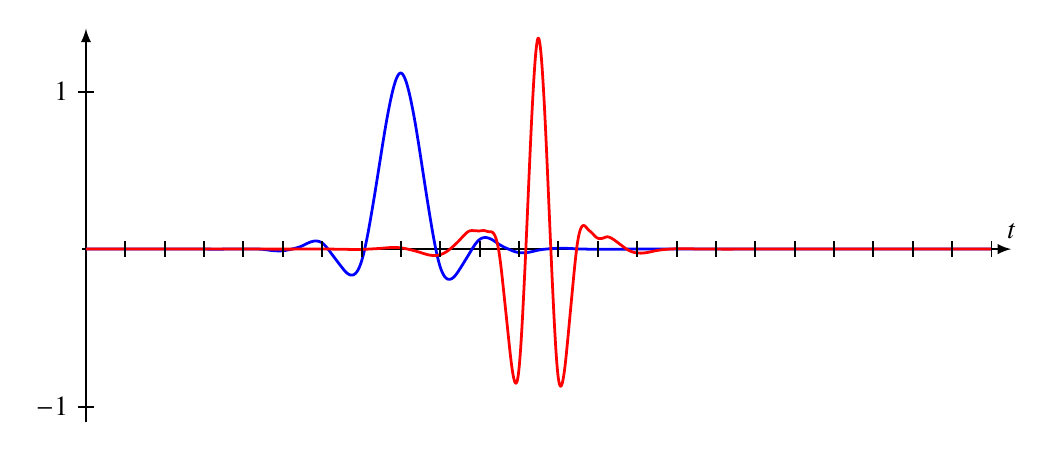
\begin{tikzpicture}[>=latex,yscale=2,xscale=0.5]

\draw[->,line width=0.7pt] (-0.1,0)--(23.5,0) coordinate[label={$t$}];
\draw[->,line width=0.7pt] (0,-1.1)--(0,1.4);

\draw[line width=1pt,color=blue] (0.00000, 0.00000)
--(0.00195, -0.00000)
--(0.00391, -0.00000)
--(0.00586, 0.00000)
--(0.00781, 0.00000)
--(0.00977, -0.00000)
--(0.01172, -0.00000)
--(0.01367, 0.00000)
--(0.01562, 0.00000)
--(0.01758, 0.00000)
--(0.01953, -0.00000)
--(0.02148, -0.00000)
--(0.02344, -0.00000)
--(0.02539, 0.00000)
--(0.02734, 0.00000)
--(0.02930, 0.00000)
--(0.03125, 0.00000)
--(0.03320, -0.00000)
--(0.03516, -0.00000)
--(0.03711, -0.00000)
--(0.03906, -0.00000)
--(0.04102, 0.00000)
--(0.04297, 0.00000)
--(0.04492, 0.00000)
--(0.04688, 0.00000)
--(0.04883, 0.00000)
--(0.05078, 0.00000)
--(0.05273, 0.00000)
--(0.05469, -0.00000)
--(0.05664, -0.00000)
--(0.05859, -0.00000)
--(0.06055, -0.00000)
--(0.06250, -0.00000)
--(0.06445, -0.00000)
--(0.06641, 0.00000)
--(0.06836, 0.00000)
--(0.07031, 0.00000)
--(0.07227, 0.00000)
--(0.07422, 0.00000)
--(0.07617, 0.00000)
--(0.07812, 0.00000)
--(0.08008, 0.00000)
--(0.08203, -0.00000)
--(0.08398, -0.00000)
--(0.08594, -0.00000)
--(0.08789, -0.00000)
--(0.08984, -0.00000)
--(0.09180, -0.00000)
--(0.09375, -0.00000)
--(0.09570, 0.00000)
--(0.09766, 0.00000)
--(0.09961, 0.00000)
--(0.10156, 0.00000)
--(0.10352, 0.00000)
--(0.10547, 0.00000)
--(0.10742, 0.00000)
--(0.10938, 0.00000)
--(0.11133, 0.00000)
--(0.11328, 0.00000)
--(0.11523, 0.00000)
--(0.11719, 0.00000)
--(0.11914, 0.00000)
--(0.12109, 0.00000)
--(0.12305, 0.00000)
--(0.12500, -0.00000)
--(0.12695, -0.00000)
--(0.12891, -0.00000)
--(0.13086, -0.00000)
--(0.13281, -0.00000)
--(0.13477, -0.00000)
--(0.13672, -0.00000)
--(0.13867, -0.00000)
--(0.14062, -0.00000)
--(0.14258, -0.00000)
--(0.14453, -0.00000)
--(0.14648, -0.00000)
--(0.14844, 0.00000)
--(0.15039, 0.00000)
--(0.15234, 0.00000)
--(0.15430, 0.00000)
--(0.15625, 0.00000)
--(0.15820, 0.00000)
--(0.16016, 0.00000)
--(0.16211, 0.00000)
--(0.16406, 0.00000)
--(0.16602, 0.00000)
--(0.16797, 0.00000)
--(0.16992, 0.00000)
--(0.17188, 0.00000)
--(0.17383, 0.00000)
--(0.17578, 0.00000)
--(0.17773, -0.00000)
--(0.17969, -0.00000)
--(0.18164, -0.00000)
--(0.18359, -0.00000)
--(0.18555, -0.00000)
--(0.18750, -0.00000)
--(0.18945, -0.00000)
--(0.19141, -0.00000)
--(0.19336, -0.00000)
--(0.19531, -0.00000)
--(0.19727, -0.00000)
--(0.19922, -0.00000)
--(0.20117, -0.00000)
--(0.20312, -0.00000)
--(0.20508, 0.00000)
--(0.20703, 0.00000)
--(0.20898, 0.00000)
--(0.21094, 0.00000)
--(0.21289, 0.00000)
--(0.21484, 0.00000)
--(0.21680, 0.00000)
--(0.21875, 0.00000)
--(0.22070, 0.00000)
--(0.22266, 0.00000)
--(0.22461, 0.00000)
--(0.22656, 0.00000)
--(0.22852, 0.00000)
--(0.23047, 0.00000)
--(0.23242, 0.00000)
--(0.23438, 0.00000)
--(0.23633, 0.00000)
--(0.23828, 0.00000)
--(0.24023, 0.00000)
--(0.24219, 0.00000)
--(0.24414, 0.00000)
--(0.24609, 0.00000)
--(0.24805, 0.00000)
--(0.25000, 0.00000)
--(0.25195, 0.00000)
--(0.25391, 0.00000)
--(0.25586, 0.00000)
--(0.25781, 0.00000)
--(0.25977, 0.00000)
--(0.26172, 0.00000)
--(0.26367, -0.00000)
--(0.26562, -0.00000)
--(0.26758, -0.00000)
--(0.26953, -0.00000)
--(0.27148, -0.00000)
--(0.27344, -0.00000)
--(0.27539, -0.00000)
--(0.27734, -0.00000)
--(0.27930, -0.00000)
--(0.28125, -0.00000)
--(0.28320, -0.00000)
--(0.28516, -0.00000)
--(0.28711, -0.00000)
--(0.28906, -0.00000)
--(0.29102, -0.00000)
--(0.29297, -0.00000)
--(0.29492, -0.00000)
--(0.29688, -0.00000)
--(0.29883, -0.00000)
--(0.30078, -0.00000)
--(0.30273, -0.00000)
--(0.30469, -0.00000)
--(0.30664, -0.00000)
--(0.30859, -0.00000)
--(0.31055, -0.00000)
--(0.31250, 0.00000)
--(0.31445, 0.00000)
--(0.31641, 0.00000)
--(0.31836, 0.00000)
--(0.32031, 0.00000)
--(0.32227, 0.00000)
--(0.32422, 0.00000)
--(0.32617, 0.00000)
--(0.32812, 0.00000)
--(0.33008, 0.00000)
--(0.33203, 0.00000)
--(0.33398, 0.00000)
--(0.33594, 0.00000)
--(0.33789, 0.00000)
--(0.33984, 0.00000)
--(0.34180, 0.00000)
--(0.34375, 0.00000)
--(0.34570, 0.00000)
--(0.34766, 0.00000)
--(0.34961, 0.00000)
--(0.35156, 0.00000)
--(0.35352, 0.00000)
--(0.35547, 0.00000)
--(0.35742, 0.00000)
--(0.35938, 0.00000)
--(0.36133, 0.00000)
--(0.36328, 0.00000)
--(0.36523, 0.00000)
--(0.36719, 0.00000)
--(0.36914, -0.00000)
--(0.37109, -0.00000)
--(0.37305, -0.00000)
--(0.37500, -0.00000)
--(0.37695, -0.00000)
--(0.37891, -0.00000)
--(0.38086, -0.00000)
--(0.38281, -0.00000)
--(0.38477, -0.00000)
--(0.38672, -0.00000)
--(0.38867, -0.00000)
--(0.39062, -0.00000)
--(0.39258, -0.00000)
--(0.39453, -0.00000)
--(0.39648, -0.00000)
--(0.39844, -0.00000)
--(0.40039, -0.00000)
--(0.40234, -0.00000)
--(0.40430, -0.00000)
--(0.40625, -0.00000)
--(0.40820, -0.00000)
--(0.41016, -0.00000)
--(0.41211, -0.00000)
--(0.41406, -0.00000)
--(0.41602, -0.00000)
--(0.41797, -0.00000)
--(0.41992, -0.00000)
--(0.42188, -0.00000)
--(0.42383, -0.00000)
--(0.42578, 0.00000)
--(0.42773, 0.00000)
--(0.42969, 0.00000)
--(0.43164, 0.00000)
--(0.43359, 0.00000)
--(0.43555, 0.00000)
--(0.43750, 0.00000)
--(0.43945, 0.00000)
--(0.44141, 0.00000)
--(0.44336, 0.00000)
--(0.44531, 0.00000)
--(0.44727, 0.00000)
--(0.44922, 0.00000)
--(0.45117, 0.00000)
--(0.45312, 0.00000)
--(0.45508, 0.00000)
--(0.45703, 0.00000)
--(0.45898, 0.00000)
--(0.46094, 0.00000)
--(0.46289, 0.00000)
--(0.46484, 0.00000)
--(0.46680, 0.00000)
--(0.46875, 0.00000)
--(0.47070, 0.00000)
--(0.47266, 0.00000)
--(0.47461, 0.00000)
--(0.47656, 0.00000)
--(0.47852, 0.00000)
--(0.48047, 0.00000)
--(0.48242, 0.00000)
--(0.48438, 0.00000)
--(0.48633, 0.00000)
--(0.48828, 0.00000)
--(0.49023, 0.00000)
--(0.49219, 0.00000)
--(0.49414, 0.00000)
--(0.49609, 0.00000)
--(0.49805, 0.00000)
--(0.50000, 0.00000)
--(0.50195, 0.00000)
--(0.50391, 0.00000)
--(0.50586, 0.00000)
--(0.50781, 0.00000)
--(0.50977, 0.00000)
--(0.51172, 0.00000)
--(0.51367, 0.00000)
--(0.51562, 0.00000)
--(0.51758, 0.00000)
--(0.51953, 0.00000)
--(0.52148, 0.00000)
--(0.52344, 0.00000)
--(0.52539, 0.00000)
--(0.52734, 0.00000)
--(0.52930, 0.00000)
--(0.53125, 0.00000)
--(0.53320, 0.00000)
--(0.53516, 0.00000)
--(0.53711, 0.00000)
--(0.53906, 0.00000)
--(0.54102, -0.00000)
--(0.54297, -0.00000)
--(0.54492, -0.00000)
--(0.54688, -0.00000)
--(0.54883, -0.00000)
--(0.55078, -0.00000)
--(0.55273, -0.00000)
--(0.55469, -0.00000)
--(0.55664, -0.00000)
--(0.55859, -0.00000)
--(0.56055, -0.00000)
--(0.56250, -0.00000)
--(0.56445, -0.00000)
--(0.56641, -0.00000)
--(0.56836, -0.00000)
--(0.57031, -0.00000)
--(0.57227, -0.00000)
--(0.57422, -0.00000)
--(0.57617, -0.00000)
--(0.57812, -0.00000)
--(0.58008, -0.00000)
--(0.58203, -0.00000)
--(0.58398, -0.00000)
--(0.58594, -0.00000)
--(0.58789, -0.00000)
--(0.58984, -0.00000)
--(0.59180, -0.00000)
--(0.59375, -0.00000)
--(0.59570, -0.00000)
--(0.59766, -0.00000)
--(0.59961, -0.00000)
--(0.60156, -0.00000)
--(0.60352, -0.00000)
--(0.60547, -0.00000)
--(0.60742, -0.00000)
--(0.60938, -0.00000)
--(0.61133, -0.00000)
--(0.61328, -0.00000)
--(0.61523, -0.00000)
--(0.61719, -0.00000)
--(0.61914, -0.00000)
--(0.62109, -0.00000)
--(0.62305, -0.00000)
--(0.62500, -0.00000)
--(0.62695, -0.00000)
--(0.62891, -0.00000)
--(0.63086, -0.00000)
--(0.63281, -0.00000)
--(0.63477, -0.00000)
--(0.63672, -0.00000)
--(0.63867, -0.00000)
--(0.64062, 0.00000)
--(0.64258, 0.00000)
--(0.64453, 0.00000)
--(0.64648, 0.00000)
--(0.64844, 0.00000)
--(0.65039, 0.00000)
--(0.65234, 0.00000)
--(0.65430, 0.00000)
--(0.65625, 0.00000)
--(0.65820, 0.00000)
--(0.66016, 0.00000)
--(0.66211, 0.00000)
--(0.66406, 0.00000)
--(0.66602, 0.00000)
--(0.66797, 0.00000)
--(0.66992, 0.00000)
--(0.67188, 0.00000)
--(0.67383, 0.00000)
--(0.67578, 0.00000)
--(0.67773, 0.00000)
--(0.67969, 0.00000)
--(0.68164, 0.00000)
--(0.68359, 0.00000)
--(0.68555, 0.00000)
--(0.68750, 0.00000)
--(0.68945, 0.00000)
--(0.69141, 0.00000)
--(0.69336, 0.00000)
--(0.69531, 0.00000)
--(0.69727, 0.00000)
--(0.69922, 0.00000)
--(0.70117, 0.00000)
--(0.70312, 0.00000)
--(0.70508, 0.00000)
--(0.70703, 0.00000)
--(0.70898, 0.00000)
--(0.71094, 0.00000)
--(0.71289, 0.00000)
--(0.71484, 0.00000)
--(0.71680, 0.00000)
--(0.71875, 0.00000)
--(0.72070, 0.00000)
--(0.72266, 0.00000)
--(0.72461, 0.00000)
--(0.72656, 0.00000)
--(0.72852, 0.00000)
--(0.73047, 0.00000)
--(0.73242, 0.00000)
--(0.73438, 0.00000)
--(0.73633, 0.00000)
--(0.73828, 0.00000)
--(0.74023, 0.00000)
--(0.74219, 0.00000)
--(0.74414, 0.00000)
--(0.74609, 0.00000)
--(0.74805, 0.00000)
--(0.75000, 0.00000)
--(0.75195, 0.00000)
--(0.75391, -0.00000)
--(0.75586, -0.00000)
--(0.75781, -0.00000)
--(0.75977, -0.00000)
--(0.76172, -0.00000)
--(0.76367, -0.00000)
--(0.76562, -0.00000)
--(0.76758, -0.00000)
--(0.76953, -0.00000)
--(0.77148, -0.00000)
--(0.77344, -0.00000)
--(0.77539, -0.00000)
--(0.77734, -0.00000)
--(0.77930, -0.00000)
--(0.78125, -0.00000)
--(0.78320, -0.00000)
--(0.78516, -0.00000)
--(0.78711, -0.00000)
--(0.78906, -0.00000)
--(0.79102, -0.00000)
--(0.79297, -0.00000)
--(0.79492, -0.00000)
--(0.79688, -0.00000)
--(0.79883, -0.00000)
--(0.80078, -0.00000)
--(0.80273, -0.00000)
--(0.80469, -0.00000)
--(0.80664, -0.00000)
--(0.80859, -0.00000)
--(0.81055, -0.00000)
--(0.81250, -0.00000)
--(0.81445, -0.00000)
--(0.81641, -0.00000)
--(0.81836, -0.00000)
--(0.82031, -0.00000)
--(0.82227, -0.00000)
--(0.82422, -0.00000)
--(0.82617, -0.00000)
--(0.82812, -0.00000)
--(0.83008, -0.00000)
--(0.83203, -0.00000)
--(0.83398, -0.00000)
--(0.83594, -0.00000)
--(0.83789, -0.00000)
--(0.83984, -0.00000)
--(0.84180, -0.00000)
--(0.84375, -0.00000)
--(0.84570, -0.00000)
--(0.84766, -0.00000)
--(0.84961, -0.00000)
--(0.85156, -0.00000)
--(0.85352, -0.00000)
--(0.85547, -0.00000)
--(0.85742, -0.00000)
--(0.85938, -0.00000)
--(0.86133, -0.00000)
--(0.86328, -0.00000)
--(0.86523, 0.00000)
--(0.86719, 0.00000)
--(0.86914, 0.00000)
--(0.87109, 0.00000)
--(0.87305, 0.00000)
--(0.87500, 0.00000)
--(0.87695, 0.00000)
--(0.87891, 0.00000)
--(0.88086, 0.00000)
--(0.88281, 0.00000)
--(0.88477, 0.00000)
--(0.88672, 0.00000)
--(0.88867, 0.00000)
--(0.89062, 0.00000)
--(0.89258, 0.00000)
--(0.89453, 0.00000)
--(0.89648, 0.00000)
--(0.89844, 0.00000)
--(0.90039, 0.00000)
--(0.90234, 0.00000)
--(0.90430, 0.00000)
--(0.90625, 0.00000)
--(0.90820, 0.00000)
--(0.91016, 0.00000)
--(0.91211, 0.00000)
--(0.91406, 0.00000)
--(0.91602, 0.00000)
--(0.91797, 0.00000)
--(0.91992, 0.00000)
--(0.92188, 0.00000)
--(0.92383, 0.00000)
--(0.92578, 0.00000)
--(0.92773, 0.00000)
--(0.92969, 0.00000)
--(0.93164, 0.00000)
--(0.93359, 0.00000)
--(0.93555, 0.00000)
--(0.93750, 0.00000)
--(0.93945, 0.00000)
--(0.94141, 0.00000)
--(0.94336, 0.00000)
--(0.94531, 0.00000)
--(0.94727, 0.00000)
--(0.94922, 0.00000)
--(0.95117, 0.00000)
--(0.95312, 0.00000)
--(0.95508, 0.00000)
--(0.95703, 0.00000)
--(0.95898, 0.00000)
--(0.96094, 0.00000)
--(0.96289, 0.00000)
--(0.96484, 0.00000)
--(0.96680, 0.00000)
--(0.96875, 0.00000)
--(0.97070, 0.00000)
--(0.97266, 0.00000)
--(0.97461, 0.00000)
--(0.97656, 0.00000)
--(0.97852, 0.00000)
--(0.98047, 0.00000)
--(0.98242, 0.00000)
--(0.98438, 0.00000)
--(0.98633, 0.00000)
--(0.98828, 0.00000)
--(0.99023, 0.00000)
--(0.99219, 0.00000)
--(0.99414, 0.00000)
--(0.99609, 0.00000)
--(0.99805, 0.00000)
--(1.00000, 0.00000)
--(1.00195, 0.00000)
--(1.00391, 0.00000)
--(1.00586, 0.00000)
--(1.00781, 0.00000)
--(1.00977, 0.00000)
--(1.01172, 0.00000)
--(1.01367, 0.00000)
--(1.01562, 0.00000)
--(1.01758, 0.00000)
--(1.01953, 0.00000)
--(1.02148, 0.00000)
--(1.02344, 0.00000)
--(1.02539, 0.00000)
--(1.02734, 0.00000)
--(1.02930, 0.00000)
--(1.03125, 0.00000)
--(1.03320, 0.00000)
--(1.03516, 0.00000)
--(1.03711, 0.00000)
--(1.03906, 0.00000)
--(1.04102, 0.00000)
--(1.04297, 0.00000)
--(1.04492, 0.00000)
--(1.04688, 0.00000)
--(1.04883, 0.00000)
--(1.05078, 0.00000)
--(1.05273, 0.00000)
--(1.05469, 0.00000)
--(1.05664, 0.00000)
--(1.05859, 0.00000)
--(1.06055, 0.00000)
--(1.06250, 0.00000)
--(1.06445, 0.00000)
--(1.06641, 0.00000)
--(1.06836, 0.00000)
--(1.07031, 0.00000)
--(1.07227, 0.00000)
--(1.07422, 0.00000)
--(1.07617, 0.00000)
--(1.07812, 0.00000)
--(1.08008, 0.00000)
--(1.08203, 0.00000)
--(1.08398, 0.00000)
--(1.08594, 0.00000)
--(1.08789, 0.00000)
--(1.08984, 0.00000)
--(1.09180, 0.00000)
--(1.09375, 0.00000)
--(1.09570, 0.00000)
--(1.09766, -0.00000)
--(1.09961, -0.00000)
--(1.10156, -0.00000)
--(1.10352, -0.00000)
--(1.10547, -0.00000)
--(1.10742, -0.00000)
--(1.10938, -0.00000)
--(1.11133, -0.00000)
--(1.11328, -0.00000)
--(1.11523, -0.00000)
--(1.11719, -0.00000)
--(1.11914, -0.00000)
--(1.12109, -0.00000)
--(1.12305, -0.00000)
--(1.12500, -0.00000)
--(1.12695, -0.00000)
--(1.12891, -0.00000)
--(1.13086, -0.00000)
--(1.13281, -0.00000)
--(1.13477, -0.00000)
--(1.13672, -0.00000)
--(1.13867, -0.00000)
--(1.14062, -0.00000)
--(1.14258, -0.00000)
--(1.14453, -0.00000)
--(1.14648, -0.00000)
--(1.14844, -0.00000)
--(1.15039, -0.00000)
--(1.15234, -0.00000)
--(1.15430, -0.00000)
--(1.15625, -0.00000)
--(1.15820, -0.00000)
--(1.16016, -0.00000)
--(1.16211, -0.00000)
--(1.16406, -0.00000)
--(1.16602, -0.00000)
--(1.16797, -0.00000)
--(1.16992, -0.00000)
--(1.17188, -0.00000)
--(1.17383, -0.00000)
--(1.17578, -0.00000)
--(1.17773, -0.00000)
--(1.17969, -0.00000)
--(1.18164, -0.00000)
--(1.18359, -0.00000)
--(1.18555, -0.00000)
--(1.18750, -0.00000)
--(1.18945, -0.00000)
--(1.19141, -0.00000)
--(1.19336, -0.00000)
--(1.19531, -0.00000)
--(1.19727, -0.00000)
--(1.19922, -0.00000)
--(1.20117, -0.00000)
--(1.20312, -0.00000)
--(1.20508, -0.00000)
--(1.20703, -0.00000)
--(1.20898, -0.00000)
--(1.21094, -0.00000)
--(1.21289, -0.00000)
--(1.21484, -0.00000)
--(1.21680, -0.00000)
--(1.21875, -0.00000)
--(1.22070, -0.00000)
--(1.22266, -0.00000)
--(1.22461, -0.00000)
--(1.22656, -0.00000)
--(1.22852, -0.00000)
--(1.23047, -0.00000)
--(1.23242, -0.00000)
--(1.23438, -0.00000)
--(1.23633, -0.00000)
--(1.23828, -0.00000)
--(1.24023, -0.00000)
--(1.24219, -0.00000)
--(1.24414, -0.00000)
--(1.24609, -0.00000)
--(1.24805, -0.00000)
--(1.25000, -0.00000)
--(1.25195, -0.00000)
--(1.25391, -0.00000)
--(1.25586, -0.00000)
--(1.25781, -0.00000)
--(1.25977, -0.00000)
--(1.26172, -0.00000)
--(1.26367, -0.00000)
--(1.26562, -0.00000)
--(1.26758, -0.00000)
--(1.26953, -0.00000)
--(1.27148, -0.00000)
--(1.27344, -0.00000)
--(1.27539, -0.00000)
--(1.27734, -0.00000)
--(1.27930, -0.00000)
--(1.28125, -0.00000)
--(1.28320, -0.00000)
--(1.28516, -0.00000)
--(1.28711, -0.00000)
--(1.28906, -0.00000)
--(1.29102, -0.00000)
--(1.29297, -0.00000)
--(1.29492, 0.00000)
--(1.29688, 0.00000)
--(1.29883, 0.00000)
--(1.30078, 0.00000)
--(1.30273, 0.00000)
--(1.30469, 0.00000)
--(1.30664, 0.00000)
--(1.30859, 0.00000)
--(1.31055, 0.00000)
--(1.31250, 0.00000)
--(1.31445, 0.00000)
--(1.31641, 0.00000)
--(1.31836, 0.00000)
--(1.32031, 0.00000)
--(1.32227, 0.00000)
--(1.32422, 0.00000)
--(1.32617, 0.00000)
--(1.32812, 0.00000)
--(1.33008, 0.00000)
--(1.33203, 0.00000)
--(1.33398, 0.00000)
--(1.33594, 0.00000)
--(1.33789, 0.00000)
--(1.33984, 0.00000)
--(1.34180, 0.00000)
--(1.34375, 0.00000)
--(1.34570, 0.00000)
--(1.34766, 0.00000)
--(1.34961, 0.00000)
--(1.35156, 0.00000)
--(1.35352, 0.00000)
--(1.35547, 0.00000)
--(1.35742, 0.00000)
--(1.35938, 0.00000)
--(1.36133, 0.00000)
--(1.36328, 0.00000)
--(1.36523, 0.00000)
--(1.36719, 0.00000)
--(1.36914, 0.00000)
--(1.37109, 0.00000)
--(1.37305, 0.00000)
--(1.37500, 0.00000)
--(1.37695, 0.00000)
--(1.37891, 0.00000)
--(1.38086, 0.00000)
--(1.38281, 0.00000)
--(1.38477, 0.00000)
--(1.38672, 0.00000)
--(1.38867, 0.00000)
--(1.39062, 0.00000)
--(1.39258, 0.00000)
--(1.39453, 0.00000)
--(1.39648, 0.00000)
--(1.39844, 0.00000)
--(1.40039, 0.00000)
--(1.40234, 0.00000)
--(1.40430, 0.00000)
--(1.40625, 0.00000)
--(1.40820, 0.00000)
--(1.41016, 0.00000)
--(1.41211, 0.00000)
--(1.41406, 0.00000)
--(1.41602, 0.00000)
--(1.41797, 0.00000)
--(1.41992, 0.00000)
--(1.42188, 0.00000)
--(1.42383, 0.00000)
--(1.42578, 0.00000)
--(1.42773, 0.00000)
--(1.42969, 0.00000)
--(1.43164, 0.00000)
--(1.43359, 0.00000)
--(1.43555, 0.00000)
--(1.43750, 0.00000)
--(1.43945, 0.00000)
--(1.44141, 0.00000)
--(1.44336, 0.00000)
--(1.44531, 0.00000)
--(1.44727, 0.00000)
--(1.44922, 0.00000)
--(1.45117, 0.00000)
--(1.45312, 0.00000)
--(1.45508, 0.00000)
--(1.45703, 0.00000)
--(1.45898, 0.00000)
--(1.46094, 0.00000)
--(1.46289, 0.00000)
--(1.46484, 0.00000)
--(1.46680, 0.00000)
--(1.46875, 0.00000)
--(1.47070, 0.00000)
--(1.47266, 0.00000)
--(1.47461, 0.00000)
--(1.47656, 0.00000)
--(1.47852, 0.00000)
--(1.48047, 0.00000)
--(1.48242, 0.00000)
--(1.48438, 0.00000)
--(1.48633, 0.00000)
--(1.48828, 0.00000)
--(1.49023, 0.00000)
--(1.49219, 0.00000)
--(1.49414, 0.00000)
--(1.49609, 0.00000)
--(1.49805, 0.00000)
--(1.50000, 0.00000)
--(1.50195, 0.00000)
--(1.50391, 0.00000)
--(1.50586, 0.00000)
--(1.50781, 0.00000)
--(1.50977, 0.00000)
--(1.51172, 0.00000)
--(1.51367, 0.00000)
--(1.51562, 0.00000)
--(1.51758, 0.00000)
--(1.51953, 0.00000)
--(1.52148, 0.00000)
--(1.52344, -0.00000)
--(1.52539, -0.00000)
--(1.52734, -0.00000)
--(1.52930, -0.00000)
--(1.53125, -0.00000)
--(1.53320, -0.00000)
--(1.53516, -0.00000)
--(1.53711, -0.00000)
--(1.53906, -0.00000)
--(1.54102, -0.00000)
--(1.54297, -0.00000)
--(1.54492, -0.00000)
--(1.54688, -0.00000)
--(1.54883, -0.00000)
--(1.55078, -0.00000)
--(1.55273, -0.00000)
--(1.55469, -0.00000)
--(1.55664, -0.00000)
--(1.55859, -0.00000)
--(1.56055, -0.00000)
--(1.56250, -0.00000)
--(1.56445, -0.00000)
--(1.56641, -0.00000)
--(1.56836, -0.00000)
--(1.57031, -0.00000)
--(1.57227, -0.00000)
--(1.57422, -0.00000)
--(1.57617, -0.00000)
--(1.57812, -0.00000)
--(1.58008, -0.00000)
--(1.58203, -0.00000)
--(1.58398, -0.00000)
--(1.58594, -0.00000)
--(1.58789, -0.00000)
--(1.58984, -0.00000)
--(1.59180, -0.00000)
--(1.59375, -0.00000)
--(1.59570, -0.00000)
--(1.59766, -0.00000)
--(1.59961, -0.00000)
--(1.60156, -0.00000)
--(1.60352, -0.00000)
--(1.60547, -0.00000)
--(1.60742, -0.00000)
--(1.60938, -0.00000)
--(1.61133, -0.00000)
--(1.61328, -0.00000)
--(1.61523, -0.00000)
--(1.61719, -0.00000)
--(1.61914, -0.00000)
--(1.62109, -0.00000)
--(1.62305, -0.00000)
--(1.62500, -0.00000)
--(1.62695, -0.00000)
--(1.62891, -0.00000)
--(1.63086, -0.00000)
--(1.63281, -0.00000)
--(1.63477, -0.00000)
--(1.63672, -0.00000)
--(1.63867, -0.00000)
--(1.64062, -0.00000)
--(1.64258, -0.00000)
--(1.64453, -0.00000)
--(1.64648, -0.00000)
--(1.64844, -0.00000)
--(1.65039, -0.00000)
--(1.65234, -0.00000)
--(1.65430, -0.00000)
--(1.65625, -0.00000)
--(1.65820, -0.00000)
--(1.66016, -0.00000)
--(1.66211, -0.00000)
--(1.66406, -0.00000)
--(1.66602, -0.00000)
--(1.66797, -0.00000)
--(1.66992, -0.00000)
--(1.67188, -0.00000)
--(1.67383, -0.00000)
--(1.67578, -0.00000)
--(1.67773, -0.00000)
--(1.67969, -0.00000)
--(1.68164, -0.00000)
--(1.68359, -0.00000)
--(1.68555, -0.00000)
--(1.68750, -0.00000)
--(1.68945, -0.00000)
--(1.69141, -0.00000)
--(1.69336, -0.00000)
--(1.69531, -0.00000)
--(1.69727, -0.00000)
--(1.69922, -0.00000)
--(1.70117, -0.00000)
--(1.70312, -0.00000)
--(1.70508, -0.00000)
--(1.70703, -0.00000)
--(1.70898, -0.00000)
--(1.71094, -0.00000)
--(1.71289, -0.00000)
--(1.71484, -0.00000)
--(1.71680, -0.00000)
--(1.71875, -0.00000)
--(1.72070, -0.00000)
--(1.72266, -0.00000)
--(1.72461, -0.00000)
--(1.72656, -0.00000)
--(1.72852, -0.00000)
--(1.73047, -0.00000)
--(1.73242, -0.00000)
--(1.73438, -0.00000)
--(1.73633, -0.00000)
--(1.73828, -0.00000)
--(1.74023, -0.00000)
--(1.74219, -0.00000)
--(1.74414, 0.00000)
--(1.74609, 0.00000)
--(1.74805, 0.00000)
--(1.75000, 0.00000)
--(1.75195, 0.00000)
--(1.75391, 0.00000)
--(1.75586, 0.00000)
--(1.75781, 0.00000)
--(1.75977, 0.00000)
--(1.76172, 0.00000)
--(1.76367, 0.00000)
--(1.76562, 0.00000)
--(1.76758, 0.00000)
--(1.76953, 0.00000)
--(1.77148, 0.00000)
--(1.77344, 0.00000)
--(1.77539, 0.00000)
--(1.77734, 0.00000)
--(1.77930, 0.00000)
--(1.78125, 0.00000)
--(1.78320, 0.00000)
--(1.78516, 0.00000)
--(1.78711, 0.00000)
--(1.78906, 0.00000)
--(1.79102, 0.00000)
--(1.79297, 0.00000)
--(1.79492, 0.00000)
--(1.79688, 0.00000)
--(1.79883, 0.00000)
--(1.80078, 0.00000)
--(1.80273, 0.00000)
--(1.80469, 0.00000)
--(1.80664, 0.00000)
--(1.80859, 0.00000)
--(1.81055, 0.00000)
--(1.81250, 0.00000)
--(1.81445, 0.00000)
--(1.81641, 0.00000)
--(1.81836, 0.00000)
--(1.82031, 0.00000)
--(1.82227, 0.00000)
--(1.82422, 0.00000)
--(1.82617, 0.00000)
--(1.82812, 0.00000)
--(1.83008, 0.00000)
--(1.83203, 0.00000)
--(1.83398, 0.00000)
--(1.83594, 0.00000)
--(1.83789, 0.00000)
--(1.83984, 0.00000)
--(1.84180, 0.00000)
--(1.84375, 0.00000)
--(1.84570, 0.00000)
--(1.84766, 0.00000)
--(1.84961, 0.00000)
--(1.85156, 0.00000)
--(1.85352, 0.00000)
--(1.85547, 0.00000)
--(1.85742, 0.00000)
--(1.85938, 0.00000)
--(1.86133, 0.00000)
--(1.86328, 0.00000)
--(1.86523, 0.00000)
--(1.86719, 0.00000)
--(1.86914, 0.00000)
--(1.87109, 0.00000)
--(1.87305, 0.00000)
--(1.87500, 0.00000)
--(1.87695, 0.00000)
--(1.87891, 0.00000)
--(1.88086, 0.00000)
--(1.88281, 0.00000)
--(1.88477, 0.00000)
--(1.88672, 0.00000)
--(1.88867, 0.00000)
--(1.89062, 0.00000)
--(1.89258, 0.00000)
--(1.89453, 0.00000)
--(1.89648, 0.00000)
--(1.89844, 0.00000)
--(1.90039, 0.00000)
--(1.90234, 0.00000)
--(1.90430, 0.00000)
--(1.90625, 0.00000)
--(1.90820, 0.00000)
--(1.91016, 0.00000)
--(1.91211, 0.00000)
--(1.91406, 0.00000)
--(1.91602, 0.00000)
--(1.91797, 0.00000)
--(1.91992, 0.00000)
--(1.92188, 0.00000)
--(1.92383, 0.00000)
--(1.92578, 0.00000)
--(1.92773, 0.00000)
--(1.92969, 0.00000)
--(1.93164, 0.00000)
--(1.93359, 0.00000)
--(1.93555, 0.00000)
--(1.93750, 0.00000)
--(1.93945, 0.00000)
--(1.94141, 0.00000)
--(1.94336, 0.00000)
--(1.94531, 0.00000)
--(1.94727, 0.00000)
--(1.94922, 0.00000)
--(1.95117, 0.00000)
--(1.95312, 0.00000)
--(1.95508, 0.00000)
--(1.95703, 0.00000)
--(1.95898, 0.00000)
--(1.96094, 0.00000)
--(1.96289, 0.00000)
--(1.96484, 0.00000)
--(1.96680, 0.00000)
--(1.96875, 0.00000)
--(1.97070, 0.00000)
--(1.97266, 0.00000)
--(1.97461, 0.00000)
--(1.97656, 0.00000)
--(1.97852, 0.00000)
--(1.98047, 0.00000)
--(1.98242, 0.00000)
--(1.98438, 0.00000)
--(1.98633, 0.00000)
--(1.98828, 0.00000)
--(1.99023, 0.00000)
--(1.99219, 0.00000)
--(1.99414, 0.00000)
--(1.99609, 0.00000)
--(1.99805, 0.00000)
--(2.00000, 0.00000)
--(2.00195, 0.00000)
--(2.00391, 0.00000)
--(2.00586, 0.00000)
--(2.00781, 0.00000)
--(2.00977, 0.00000)
--(2.01172, 0.00000)
--(2.01367, 0.00000)
--(2.01562, 0.00000)
--(2.01758, 0.00000)
--(2.01953, 0.00000)
--(2.02148, 0.00000)
--(2.02344, 0.00000)
--(2.02539, 0.00000)
--(2.02734, 0.00000)
--(2.02930, 0.00000)
--(2.03125, 0.00000)
--(2.03320, 0.00000)
--(2.03516, 0.00000)
--(2.03711, 0.00000)
--(2.03906, 0.00000)
--(2.04102, 0.00000)
--(2.04297, 0.00000)
--(2.04492, 0.00000)
--(2.04688, 0.00000)
--(2.04883, 0.00000)
--(2.05078, 0.00000)
--(2.05273, 0.00000)
--(2.05469, 0.00000)
--(2.05664, 0.00000)
--(2.05859, 0.00000)
--(2.06055, 0.00000)
--(2.06250, 0.00000)
--(2.06445, 0.00000)
--(2.06641, 0.00000)
--(2.06836, 0.00000)
--(2.07031, 0.00000)
--(2.07227, 0.00000)
--(2.07422, 0.00000)
--(2.07617, 0.00000)
--(2.07812, 0.00000)
--(2.08008, 0.00000)
--(2.08203, 0.00000)
--(2.08398, 0.00000)
--(2.08594, 0.00000)
--(2.08789, 0.00000)
--(2.08984, 0.00000)
--(2.09180, 0.00000)
--(2.09375, 0.00000)
--(2.09570, 0.00000)
--(2.09766, 0.00000)
--(2.09961, 0.00000)
--(2.10156, 0.00000)
--(2.10352, 0.00000)
--(2.10547, 0.00000)
--(2.10742, 0.00000)
--(2.10938, 0.00000)
--(2.11133, 0.00000)
--(2.11328, 0.00000)
--(2.11523, 0.00000)
--(2.11719, 0.00000)
--(2.11914, 0.00000)
--(2.12109, 0.00000)
--(2.12305, 0.00000)
--(2.12500, 0.00000)
--(2.12695, 0.00000)
--(2.12891, 0.00000)
--(2.13086, 0.00000)
--(2.13281, 0.00000)
--(2.13477, 0.00000)
--(2.13672, 0.00000)
--(2.13867, 0.00000)
--(2.14062, 0.00000)
--(2.14258, 0.00000)
--(2.14453, 0.00000)
--(2.14648, 0.00000)
--(2.14844, 0.00000)
--(2.15039, 0.00000)
--(2.15234, 0.00000)
--(2.15430, 0.00000)
--(2.15625, 0.00000)
--(2.15820, 0.00000)
--(2.16016, 0.00000)
--(2.16211, 0.00000)
--(2.16406, 0.00000)
--(2.16602, 0.00000)
--(2.16797, 0.00000)
--(2.16992, 0.00000)
--(2.17188, 0.00000)
--(2.17383, 0.00000)
--(2.17578, 0.00000)
--(2.17773, 0.00000)
--(2.17969, 0.00000)
--(2.18164, 0.00000)
--(2.18359, 0.00000)
--(2.18555, 0.00000)
--(2.18750, 0.00000)
--(2.18945, 0.00000)
--(2.19141, 0.00000)
--(2.19336, 0.00000)
--(2.19531, 0.00000)
--(2.19727, 0.00000)
--(2.19922, 0.00000)
--(2.20117, 0.00000)
--(2.20312, 0.00000)
--(2.20508, 0.00000)
--(2.20703, 0.00000)
--(2.20898, 0.00000)
--(2.21094, -0.00000)
--(2.21289, -0.00000)
--(2.21484, -0.00000)
--(2.21680, -0.00000)
--(2.21875, -0.00000)
--(2.22070, -0.00000)
--(2.22266, -0.00000)
--(2.22461, -0.00000)
--(2.22656, -0.00000)
--(2.22852, -0.00000)
--(2.23047, -0.00000)
--(2.23242, -0.00000)
--(2.23438, -0.00000)
--(2.23633, -0.00000)
--(2.23828, -0.00000)
--(2.24023, -0.00000)
--(2.24219, -0.00000)
--(2.24414, -0.00000)
--(2.24609, -0.00000)
--(2.24805, -0.00000)
--(2.25000, -0.00000)
--(2.25195, -0.00000)
--(2.25391, -0.00000)
--(2.25586, -0.00000)
--(2.25781, -0.00000)
--(2.25977, -0.00000)
--(2.26172, -0.00000)
--(2.26367, -0.00000)
--(2.26562, -0.00000)
--(2.26758, -0.00000)
--(2.26953, -0.00000)
--(2.27148, -0.00000)
--(2.27344, -0.00000)
--(2.27539, -0.00001)
--(2.27734, -0.00001)
--(2.27930, -0.00001)
--(2.28125, -0.00001)
--(2.28320, -0.00001)
--(2.28516, -0.00001)
--(2.28711, -0.00001)
--(2.28906, -0.00001)
--(2.29102, -0.00001)
--(2.29297, -0.00001)
--(2.29492, -0.00001)
--(2.29688, -0.00001)
--(2.29883, -0.00001)
--(2.30078, -0.00001)
--(2.30273, -0.00001)
--(2.30469, -0.00001)
--(2.30664, -0.00001)
--(2.30859, -0.00001)
--(2.31055, -0.00001)
--(2.31250, -0.00001)
--(2.31445, -0.00001)
--(2.31641, -0.00001)
--(2.31836, -0.00001)
--(2.32031, -0.00001)
--(2.32227, -0.00001)
--(2.32422, -0.00001)
--(2.32617, -0.00001)
--(2.32812, -0.00001)
--(2.33008, -0.00001)
--(2.33203, -0.00001)
--(2.33398, -0.00001)
--(2.33594, -0.00001)
--(2.33789, -0.00001)
--(2.33984, -0.00001)
--(2.34180, -0.00001)
--(2.34375, -0.00001)
--(2.34570, -0.00001)
--(2.34766, -0.00001)
--(2.34961, -0.00001)
--(2.35156, -0.00001)
--(2.35352, -0.00001)
--(2.35547, -0.00001)
--(2.35742, -0.00001)
--(2.35938, -0.00001)
--(2.36133, -0.00001)
--(2.36328, -0.00001)
--(2.36523, -0.00001)
--(2.36719, -0.00001)
--(2.36914, -0.00001)
--(2.37109, -0.00001)
--(2.37305, -0.00001)
--(2.37500, -0.00001)
--(2.37695, -0.00002)
--(2.37891, -0.00002)
--(2.38086, -0.00002)
--(2.38281, -0.00002)
--(2.38477, -0.00002)
--(2.38672, -0.00002)
--(2.38867, -0.00002)
--(2.39062, -0.00002)
--(2.39258, -0.00002)
--(2.39453, -0.00002)
--(2.39648, -0.00002)
--(2.39844, -0.00002)
--(2.40039, -0.00002)
--(2.40234, -0.00002)
--(2.40430, -0.00002)
--(2.40625, -0.00002)
--(2.40820, -0.00002)
--(2.41016, -0.00002)
--(2.41211, -0.00002)
--(2.41406, -0.00002)
--(2.41602, -0.00002)
--(2.41797, -0.00002)
--(2.41992, -0.00002)
--(2.42188, -0.00002)
--(2.42383, -0.00002)
--(2.42578, -0.00002)
--(2.42773, -0.00002)
--(2.42969, -0.00002)
--(2.43164, -0.00002)
--(2.43359, -0.00002)
--(2.43555, -0.00002)
--(2.43750, -0.00002)
--(2.43945, -0.00002)
--(2.44141, -0.00002)
--(2.44336, -0.00002)
--(2.44531, -0.00002)
--(2.44727, -0.00002)
--(2.44922, -0.00002)
--(2.45117, -0.00002)
--(2.45312, -0.00002)
--(2.45508, -0.00002)
--(2.45703, -0.00002)
--(2.45898, -0.00002)
--(2.46094, -0.00002)
--(2.46289, -0.00002)
--(2.46484, -0.00002)
--(2.46680, -0.00002)
--(2.46875, -0.00002)
--(2.47070, -0.00002)
--(2.47266, -0.00002)
--(2.47461, -0.00002)
--(2.47656, -0.00002)
--(2.47852, -0.00002)
--(2.48047, -0.00002)
--(2.48242, -0.00002)
--(2.48438, -0.00002)
--(2.48633, -0.00002)
--(2.48828, -0.00002)
--(2.49023, -0.00002)
--(2.49219, -0.00002)
--(2.49414, -0.00002)
--(2.49609, -0.00002)
--(2.49805, -0.00002)
--(2.50000, -0.00002)
--(2.50195, -0.00002)
--(2.50391, -0.00001)
--(2.50586, -0.00001)
--(2.50781, -0.00001)
--(2.50977, -0.00001)
--(2.51172, -0.00001)
--(2.51367, -0.00001)
--(2.51562, -0.00001)
--(2.51758, -0.00001)
--(2.51953, -0.00001)
--(2.52148, -0.00001)
--(2.52344, -0.00001)
--(2.52539, -0.00001)
--(2.52734, -0.00001)
--(2.52930, -0.00001)
--(2.53125, -0.00001)
--(2.53320, -0.00001)
--(2.53516, -0.00001)
--(2.53711, -0.00001)
--(2.53906, -0.00001)
--(2.54102, -0.00001)
--(2.54297, -0.00001)
--(2.54492, -0.00001)
--(2.54688, -0.00001)
--(2.54883, -0.00001)
--(2.55078, -0.00001)
--(2.55273, -0.00001)
--(2.55469, -0.00001)
--(2.55664, -0.00001)
--(2.55859, -0.00001)
--(2.56055, -0.00001)
--(2.56250, -0.00001)
--(2.56445, -0.00001)
--(2.56641, -0.00001)
--(2.56836, -0.00001)
--(2.57031, -0.00001)
--(2.57227, -0.00001)
--(2.57422, -0.00001)
--(2.57617, -0.00001)
--(2.57812, -0.00000)
--(2.58008, -0.00000)
--(2.58203, -0.00000)
--(2.58398, -0.00000)
--(2.58594, -0.00000)
--(2.58789, -0.00000)
--(2.58984, -0.00000)
--(2.59180, -0.00000)
--(2.59375, -0.00000)
--(2.59570, -0.00000)
--(2.59766, -0.00000)
--(2.59961, -0.00000)
--(2.60156, -0.00000)
--(2.60352, -0.00000)
--(2.60547, -0.00000)
--(2.60742, 0.00000)
--(2.60938, 0.00000)
--(2.61133, 0.00000)
--(2.61328, 0.00000)
--(2.61523, 0.00000)
--(2.61719, 0.00000)
--(2.61914, 0.00000)
--(2.62109, 0.00000)
--(2.62305, 0.00000)
--(2.62500, 0.00000)
--(2.62695, 0.00000)
--(2.62891, 0.00000)
--(2.63086, 0.00000)
--(2.63281, 0.00000)
--(2.63477, 0.00000)
--(2.63672, 0.00001)
--(2.63867, 0.00001)
--(2.64062, 0.00001)
--(2.64258, 0.00001)
--(2.64453, 0.00001)
--(2.64648, 0.00001)
--(2.64844, 0.00001)
--(2.65039, 0.00001)
--(2.65234, 0.00001)
--(2.65430, 0.00001)
--(2.65625, 0.00001)
--(2.65820, 0.00001)
--(2.66016, 0.00001)
--(2.66211, 0.00001)
--(2.66406, 0.00001)
--(2.66602, 0.00001)
--(2.66797, 0.00001)
--(2.66992, 0.00001)
--(2.67188, 0.00001)
--(2.67383, 0.00001)
--(2.67578, 0.00001)
--(2.67773, 0.00001)
--(2.67969, 0.00001)
--(2.68164, 0.00001)
--(2.68359, 0.00001)
--(2.68555, 0.00001)
--(2.68750, 0.00002)
--(2.68945, 0.00002)
--(2.69141, 0.00002)
--(2.69336, 0.00002)
--(2.69531, 0.00002)
--(2.69727, 0.00002)
--(2.69922, 0.00002)
--(2.70117, 0.00002)
--(2.70312, 0.00002)
--(2.70508, 0.00002)
--(2.70703, 0.00002)
--(2.70898, 0.00002)
--(2.71094, 0.00002)
--(2.71289, 0.00002)
--(2.71484, 0.00002)
--(2.71680, 0.00002)
--(2.71875, 0.00002)
--(2.72070, 0.00002)
--(2.72266, 0.00002)
--(2.72461, 0.00003)
--(2.72656, 0.00003)
--(2.72852, 0.00003)
--(2.73047, 0.00003)
--(2.73242, 0.00003)
--(2.73438, 0.00003)
--(2.73633, 0.00003)
--(2.73828, 0.00003)
--(2.74023, 0.00003)
--(2.74219, 0.00003)
--(2.74414, 0.00003)
--(2.74609, 0.00003)
--(2.74805, 0.00003)
--(2.75000, 0.00003)
--(2.75195, 0.00003)
--(2.75391, 0.00004)
--(2.75586, 0.00004)
--(2.75781, 0.00004)
--(2.75977, 0.00004)
--(2.76172, 0.00004)
--(2.76367, 0.00004)
--(2.76562, 0.00004)
--(2.76758, 0.00004)
--(2.76953, 0.00004)
--(2.77148, 0.00004)
--(2.77344, 0.00004)
--(2.77539, 0.00004)
--(2.77734, 0.00004)
--(2.77930, 0.00005)
--(2.78125, 0.00005)
--(2.78320, 0.00005)
--(2.78516, 0.00005)
--(2.78711, 0.00005)
--(2.78906, 0.00005)
--(2.79102, 0.00005)
--(2.79297, 0.00005)
--(2.79492, 0.00005)
--(2.79688, 0.00005)
--(2.79883, 0.00005)
--(2.80078, 0.00005)
--(2.80273, 0.00006)
--(2.80469, 0.00006)
--(2.80664, 0.00006)
--(2.80859, 0.00006)
--(2.81055, 0.00006)
--(2.81250, 0.00006)
--(2.81445, 0.00006)
--(2.81641, 0.00006)
--(2.81836, 0.00006)
--(2.82031, 0.00006)
--(2.82227, 0.00006)
--(2.82422, 0.00006)
--(2.82617, 0.00006)
--(2.82812, 0.00006)
--(2.83008, 0.00007)
--(2.83203, 0.00007)
--(2.83398, 0.00007)
--(2.83594, 0.00007)
--(2.83789, 0.00007)
--(2.83984, 0.00007)
--(2.84180, 0.00007)
--(2.84375, 0.00007)
--(2.84570, 0.00007)
--(2.84766, 0.00007)
--(2.84961, 0.00007)
--(2.85156, 0.00007)
--(2.85352, 0.00007)
--(2.85547, 0.00007)
--(2.85742, 0.00007)
--(2.85938, 0.00007)
--(2.86133, 0.00007)
--(2.86328, 0.00008)
--(2.86523, 0.00008)
--(2.86719, 0.00008)
--(2.86914, 0.00008)
--(2.87109, 0.00008)
--(2.87305, 0.00008)
--(2.87500, 0.00008)
--(2.87695, 0.00008)
--(2.87891, 0.00008)
--(2.88086, 0.00008)
--(2.88281, 0.00008)
--(2.88477, 0.00008)
--(2.88672, 0.00008)
--(2.88867, 0.00008)
--(2.89062, 0.00008)
--(2.89258, 0.00008)
--(2.89453, 0.00008)
--(2.89648, 0.00008)
--(2.89844, 0.00008)
--(2.90039, 0.00008)
--(2.90234, 0.00008)
--(2.90430, 0.00008)
--(2.90625, 0.00008)
--(2.90820, 0.00008)
--(2.91016, 0.00008)
--(2.91211, 0.00008)
--(2.91406, 0.00008)
--(2.91602, 0.00008)
--(2.91797, 0.00008)
--(2.91992, 0.00008)
--(2.92188, 0.00008)
--(2.92383, 0.00008)
--(2.92578, 0.00008)
--(2.92773, 0.00008)
--(2.92969, 0.00008)
--(2.93164, 0.00008)
--(2.93359, 0.00008)
--(2.93555, 0.00008)
--(2.93750, 0.00008)
--(2.93945, 0.00008)
--(2.94141, 0.00008)
--(2.94336, 0.00008)
--(2.94531, 0.00008)
--(2.94727, 0.00008)
--(2.94922, 0.00008)
--(2.95117, 0.00008)
--(2.95312, 0.00008)
--(2.95508, 0.00008)
--(2.95703, 0.00008)
--(2.95898, 0.00008)
--(2.96094, 0.00008)
--(2.96289, 0.00008)
--(2.96484, 0.00008)
--(2.96680, 0.00008)
--(2.96875, 0.00007)
--(2.97070, 0.00007)
--(2.97266, 0.00007)
--(2.97461, 0.00007)
--(2.97656, 0.00007)
--(2.97852, 0.00007)
--(2.98047, 0.00007)
--(2.98242, 0.00007)
--(2.98438, 0.00007)
--(2.98633, 0.00007)
--(2.98828, 0.00007)
--(2.99023, 0.00006)
--(2.99219, 0.00006)
--(2.99414, 0.00006)
--(2.99609, 0.00006)
--(2.99805, 0.00006)
--(3.00000, 0.00006)
--(3.00195, 0.00006)
--(3.00391, 0.00006)
--(3.00586, 0.00005)
--(3.00781, 0.00005)
--(3.00977, 0.00005)
--(3.01172, 0.00005)
--(3.01367, 0.00005)
--(3.01562, 0.00005)
--(3.01758, 0.00004)
--(3.01953, 0.00004)
--(3.02148, 0.00004)
--(3.02344, 0.00004)
--(3.02539, 0.00004)
--(3.02734, 0.00004)
--(3.02930, 0.00003)
--(3.03125, 0.00003)
--(3.03320, 0.00003)
--(3.03516, 0.00003)
--(3.03711, 0.00003)
--(3.03906, 0.00002)
--(3.04102, 0.00002)
--(3.04297, 0.00002)
--(3.04492, 0.00002)
--(3.04688, 0.00002)
--(3.04883, 0.00001)
--(3.05078, 0.00001)
--(3.05273, 0.00001)
--(3.05469, 0.00001)
--(3.05664, 0.00001)
--(3.05859, 0.00000)
--(3.06055, 0.00000)
--(3.06250, 0.00000)
--(3.06445, -0.00000)
--(3.06641, -0.00000)
--(3.06836, -0.00001)
--(3.07031, -0.00001)
--(3.07227, -0.00001)
--(3.07422, -0.00001)
--(3.07617, -0.00001)
--(3.07812, -0.00002)
--(3.08008, -0.00002)
--(3.08203, -0.00002)
--(3.08398, -0.00002)
--(3.08594, -0.00003)
--(3.08789, -0.00003)
--(3.08984, -0.00003)
--(3.09180, -0.00003)
--(3.09375, -0.00003)
--(3.09570, -0.00004)
--(3.09766, -0.00004)
--(3.09961, -0.00004)
--(3.10156, -0.00004)
--(3.10352, -0.00005)
--(3.10547, -0.00005)
--(3.10742, -0.00005)
--(3.10938, -0.00005)
--(3.11133, -0.00005)
--(3.11328, -0.00006)
--(3.11523, -0.00006)
--(3.11719, -0.00006)
--(3.11914, -0.00006)
--(3.12109, -0.00007)
--(3.12305, -0.00007)
--(3.12500, -0.00007)
--(3.12695, -0.00007)
--(3.12891, -0.00007)
--(3.13086, -0.00008)
--(3.13281, -0.00008)
--(3.13477, -0.00008)
--(3.13672, -0.00008)
--(3.13867, -0.00008)
--(3.14062, -0.00009)
--(3.14258, -0.00009)
--(3.14453, -0.00009)
--(3.14648, -0.00009)
--(3.14844, -0.00009)
--(3.15039, -0.00010)
--(3.15234, -0.00010)
--(3.15430, -0.00010)
--(3.15625, -0.00010)
--(3.15820, -0.00010)
--(3.16016, -0.00011)
--(3.16211, -0.00011)
--(3.16406, -0.00011)
--(3.16602, -0.00011)
--(3.16797, -0.00011)
--(3.16992, -0.00012)
--(3.17188, -0.00012)
--(3.17383, -0.00012)
--(3.17578, -0.00012)
--(3.17773, -0.00012)
--(3.17969, -0.00013)
--(3.18164, -0.00013)
--(3.18359, -0.00013)
--(3.18555, -0.00013)
--(3.18750, -0.00013)
--(3.18945, -0.00014)
--(3.19141, -0.00014)
--(3.19336, -0.00014)
--(3.19531, -0.00014)
--(3.19727, -0.00014)
--(3.19922, -0.00014)
--(3.20117, -0.00015)
--(3.20312, -0.00015)
--(3.20508, -0.00015)
--(3.20703, -0.00015)
--(3.20898, -0.00015)
--(3.21094, -0.00015)
--(3.21289, -0.00016)
--(3.21484, -0.00016)
--(3.21680, -0.00016)
--(3.21875, -0.00016)
--(3.22070, -0.00016)
--(3.22266, -0.00016)
--(3.22461, -0.00017)
--(3.22656, -0.00017)
--(3.22852, -0.00017)
--(3.23047, -0.00017)
--(3.23242, -0.00017)
--(3.23438, -0.00017)
--(3.23633, -0.00017)
--(3.23828, -0.00018)
--(3.24023, -0.00018)
--(3.24219, -0.00018)
--(3.24414, -0.00018)
--(3.24609, -0.00018)
--(3.24805, -0.00018)
--(3.25000, -0.00018)
--(3.25195, -0.00018)
--(3.25391, -0.00019)
--(3.25586, -0.00019)
--(3.25781, -0.00019)
--(3.25977, -0.00019)
--(3.26172, -0.00019)
--(3.26367, -0.00019)
--(3.26562, -0.00019)
--(3.26758, -0.00019)
--(3.26953, -0.00019)
--(3.27148, -0.00020)
--(3.27344, -0.00020)
--(3.27539, -0.00020)
--(3.27734, -0.00020)
--(3.27930, -0.00020)
--(3.28125, -0.00020)
--(3.28320, -0.00020)
--(3.28516, -0.00020)
--(3.28711, -0.00020)
--(3.28906, -0.00020)
--(3.29102, -0.00020)
--(3.29297, -0.00020)
--(3.29492, -0.00020)
--(3.29688, -0.00020)
--(3.29883, -0.00020)
--(3.30078, -0.00021)
--(3.30273, -0.00021)
--(3.30469, -0.00021)
--(3.30664, -0.00021)
--(3.30859, -0.00021)
--(3.31055, -0.00021)
--(3.31250, -0.00021)
--(3.31445, -0.00021)
--(3.31641, -0.00021)
--(3.31836, -0.00021)
--(3.32031, -0.00021)
--(3.32227, -0.00021)
--(3.32422, -0.00021)
--(3.32617, -0.00021)
--(3.32812, -0.00021)
--(3.33008, -0.00021)
--(3.33203, -0.00021)
--(3.33398, -0.00021)
--(3.33594, -0.00021)
--(3.33789, -0.00021)
--(3.33984, -0.00021)
--(3.34180, -0.00021)
--(3.34375, -0.00021)
--(3.34570, -0.00021)
--(3.34766, -0.00021)
--(3.34961, -0.00021)
--(3.35156, -0.00020)
--(3.35352, -0.00020)
--(3.35547, -0.00020)
--(3.35742, -0.00020)
--(3.35938, -0.00020)
--(3.36133, -0.00020)
--(3.36328, -0.00020)
--(3.36523, -0.00020)
--(3.36719, -0.00020)
--(3.36914, -0.00020)
--(3.37109, -0.00020)
--(3.37305, -0.00020)
--(3.37500, -0.00020)
--(3.37695, -0.00020)
--(3.37891, -0.00020)
--(3.38086, -0.00020)
--(3.38281, -0.00019)
--(3.38477, -0.00019)
--(3.38672, -0.00019)
--(3.38867, -0.00019)
--(3.39062, -0.00019)
--(3.39258, -0.00019)
--(3.39453, -0.00019)
--(3.39648, -0.00019)
--(3.39844, -0.00019)
--(3.40039, -0.00019)
--(3.40234, -0.00018)
--(3.40430, -0.00018)
--(3.40625, -0.00018)
--(3.40820, -0.00018)
--(3.41016, -0.00018)
--(3.41211, -0.00018)
--(3.41406, -0.00017)
--(3.41602, -0.00017)
--(3.41797, -0.00017)
--(3.41992, -0.00017)
--(3.42188, -0.00017)
--(3.42383, -0.00017)
--(3.42578, -0.00016)
--(3.42773, -0.00016)
--(3.42969, -0.00016)
--(3.43164, -0.00016)
--(3.43359, -0.00016)
--(3.43555, -0.00015)
--(3.43750, -0.00015)
--(3.43945, -0.00015)
--(3.44141, -0.00015)
--(3.44336, -0.00014)
--(3.44531, -0.00014)
--(3.44727, -0.00014)
--(3.44922, -0.00013)
--(3.45117, -0.00013)
--(3.45312, -0.00013)
--(3.45508, -0.00013)
--(3.45703, -0.00012)
--(3.45898, -0.00012)
--(3.46094, -0.00012)
--(3.46289, -0.00011)
--(3.46484, -0.00011)
--(3.46680, -0.00011)
--(3.46875, -0.00010)
--(3.47070, -0.00010)
--(3.47266, -0.00010)
--(3.47461, -0.00009)
--(3.47656, -0.00009)
--(3.47852, -0.00008)
--(3.48047, -0.00008)
--(3.48242, -0.00008)
--(3.48438, -0.00007)
--(3.48633, -0.00007)
--(3.48828, -0.00006)
--(3.49023, -0.00006)
--(3.49219, -0.00005)
--(3.49414, -0.00005)
--(3.49609, -0.00004)
--(3.49805, -0.00004)
--(3.50000, -0.00003)
--(3.50195, -0.00003)
--(3.50391, -0.00002)
--(3.50586, -0.00002)
--(3.50781, -0.00001)
--(3.50977, -0.00001)
--(3.51172, -0.00000)
--(3.51367, 0.00000)
--(3.51562, 0.00001)
--(3.51758, 0.00001)
--(3.51953, 0.00002)
--(3.52148, 0.00003)
--(3.52344, 0.00003)
--(3.52539, 0.00004)
--(3.52734, 0.00004)
--(3.52930, 0.00005)
--(3.53125, 0.00005)
--(3.53320, 0.00006)
--(3.53516, 0.00007)
--(3.53711, 0.00007)
--(3.53906, 0.00008)
--(3.54102, 0.00009)
--(3.54297, 0.00009)
--(3.54492, 0.00010)
--(3.54688, 0.00010)
--(3.54883, 0.00011)
--(3.55078, 0.00012)
--(3.55273, 0.00012)
--(3.55469, 0.00013)
--(3.55664, 0.00014)
--(3.55859, 0.00014)
--(3.56055, 0.00015)
--(3.56250, 0.00016)
--(3.56445, 0.00016)
--(3.56641, 0.00017)
--(3.56836, 0.00018)
--(3.57031, 0.00018)
--(3.57227, 0.00019)
--(3.57422, 0.00020)
--(3.57617, 0.00020)
--(3.57812, 0.00021)
--(3.58008, 0.00022)
--(3.58203, 0.00023)
--(3.58398, 0.00023)
--(3.58594, 0.00024)
--(3.58789, 0.00025)
--(3.58984, 0.00025)
--(3.59180, 0.00026)
--(3.59375, 0.00027)
--(3.59570, 0.00028)
--(3.59766, 0.00028)
--(3.59961, 0.00029)
--(3.60156, 0.00030)
--(3.60352, 0.00030)
--(3.60547, 0.00031)
--(3.60742, 0.00032)
--(3.60938, 0.00033)
--(3.61133, 0.00033)
--(3.61328, 0.00034)
--(3.61523, 0.00035)
--(3.61719, 0.00036)
--(3.61914, 0.00036)
--(3.62109, 0.00037)
--(3.62305, 0.00038)
--(3.62500, 0.00039)
--(3.62695, 0.00039)
--(3.62891, 0.00040)
--(3.63086, 0.00041)
--(3.63281, 0.00042)
--(3.63477, 0.00042)
--(3.63672, 0.00043)
--(3.63867, 0.00044)
--(3.64062, 0.00045)
--(3.64258, 0.00045)
--(3.64453, 0.00046)
--(3.64648, 0.00047)
--(3.64844, 0.00048)
--(3.65039, 0.00048)
--(3.65234, 0.00049)
--(3.65430, 0.00050)
--(3.65625, 0.00051)
--(3.65820, 0.00051)
--(3.66016, 0.00052)
--(3.66211, 0.00053)
--(3.66406, 0.00054)
--(3.66602, 0.00054)
--(3.66797, 0.00055)
--(3.66992, 0.00056)
--(3.67188, 0.00056)
--(3.67383, 0.00057)
--(3.67578, 0.00058)
--(3.67773, 0.00058)
--(3.67969, 0.00059)
--(3.68164, 0.00060)
--(3.68359, 0.00061)
--(3.68555, 0.00061)
--(3.68750, 0.00062)
--(3.68945, 0.00063)
--(3.69141, 0.00063)
--(3.69336, 0.00064)
--(3.69531, 0.00065)
--(3.69727, 0.00065)
--(3.69922, 0.00066)
--(3.70117, 0.00066)
--(3.70312, 0.00067)
--(3.70508, 0.00068)
--(3.70703, 0.00068)
--(3.70898, 0.00069)
--(3.71094, 0.00069)
--(3.71289, 0.00070)
--(3.71484, 0.00071)
--(3.71680, 0.00071)
--(3.71875, 0.00072)
--(3.72070, 0.00072)
--(3.72266, 0.00073)
--(3.72461, 0.00073)
--(3.72656, 0.00074)
--(3.72852, 0.00074)
--(3.73047, 0.00075)
--(3.73242, 0.00075)
--(3.73438, 0.00076)
--(3.73633, 0.00076)
--(3.73828, 0.00077)
--(3.74023, 0.00077)
--(3.74219, 0.00077)
--(3.74414, 0.00078)
--(3.74609, 0.00078)
--(3.74805, 0.00079)
--(3.75000, 0.00079)
--(3.75195, 0.00079)
--(3.75391, 0.00080)
--(3.75586, 0.00080)
--(3.75781, 0.00080)
--(3.75977, 0.00081)
--(3.76172, 0.00081)
--(3.76367, 0.00081)
--(3.76562, 0.00082)
--(3.76758, 0.00082)
--(3.76953, 0.00082)
--(3.77148, 0.00082)
--(3.77344, 0.00083)
--(3.77539, 0.00083)
--(3.77734, 0.00083)
--(3.77930, 0.00083)
--(3.78125, 0.00084)
--(3.78320, 0.00084)
--(3.78516, 0.00084)
--(3.78711, 0.00084)
--(3.78906, 0.00084)
--(3.79102, 0.00085)
--(3.79297, 0.00085)
--(3.79492, 0.00085)
--(3.79688, 0.00085)
--(3.79883, 0.00085)
--(3.80078, 0.00086)
--(3.80273, 0.00086)
--(3.80469, 0.00086)
--(3.80664, 0.00086)
--(3.80859, 0.00086)
--(3.81055, 0.00086)
--(3.81250, 0.00086)
--(3.81445, 0.00087)
--(3.81641, 0.00087)
--(3.81836, 0.00087)
--(3.82031, 0.00087)
--(3.82227, 0.00087)
--(3.82422, 0.00087)
--(3.82617, 0.00087)
--(3.82812, 0.00087)
--(3.83008, 0.00088)
--(3.83203, 0.00088)
--(3.83398, 0.00088)
--(3.83594, 0.00088)
--(3.83789, 0.00088)
--(3.83984, 0.00088)
--(3.84180, 0.00088)
--(3.84375, 0.00088)
--(3.84570, 0.00088)
--(3.84766, 0.00089)
--(3.84961, 0.00089)
--(3.85156, 0.00089)
--(3.85352, 0.00089)
--(3.85547, 0.00089)
--(3.85742, 0.00089)
--(3.85938, 0.00089)
--(3.86133, 0.00089)
--(3.86328, 0.00089)
--(3.86523, 0.00089)
--(3.86719, 0.00090)
--(3.86914, 0.00090)
--(3.87109, 0.00090)
--(3.87305, 0.00090)
--(3.87500, 0.00090)
--(3.87695, 0.00090)
--(3.87891, 0.00090)
--(3.88086, 0.00090)
--(3.88281, 0.00090)
--(3.88477, 0.00090)
--(3.88672, 0.00091)
--(3.88867, 0.00091)
--(3.89062, 0.00091)
--(3.89258, 0.00091)
--(3.89453, 0.00091)
--(3.89648, 0.00091)
--(3.89844, 0.00091)
--(3.90039, 0.00091)
--(3.90234, 0.00092)
--(3.90430, 0.00092)
--(3.90625, 0.00092)
--(3.90820, 0.00092)
--(3.91016, 0.00092)
--(3.91211, 0.00092)
--(3.91406, 0.00092)
--(3.91602, 0.00092)
--(3.91797, 0.00092)
--(3.91992, 0.00093)
--(3.92188, 0.00093)
--(3.92383, 0.00093)
--(3.92578, 0.00093)
--(3.92773, 0.00093)
--(3.92969, 0.00093)
--(3.93164, 0.00093)
--(3.93359, 0.00093)
--(3.93555, 0.00094)
--(3.93750, 0.00094)
--(3.93945, 0.00094)
--(3.94141, 0.00094)
--(3.94336, 0.00094)
--(3.94531, 0.00094)
--(3.94727, 0.00094)
--(3.94922, 0.00094)
--(3.95117, 0.00095)
--(3.95312, 0.00095)
--(3.95508, 0.00095)
--(3.95703, 0.00095)
--(3.95898, 0.00095)
--(3.96094, 0.00095)
--(3.96289, 0.00095)
--(3.96484, 0.00096)
--(3.96680, 0.00096)
--(3.96875, 0.00096)
--(3.97070, 0.00096)
--(3.97266, 0.00096)
--(3.97461, 0.00097)
--(3.97656, 0.00097)
--(3.97852, 0.00097)
--(3.98047, 0.00097)
--(3.98242, 0.00097)
--(3.98438, 0.00098)
--(3.98633, 0.00098)
--(3.98828, 0.00098)
--(3.99023, 0.00098)
--(3.99219, 0.00098)
--(3.99414, 0.00099)
--(3.99609, 0.00099)
--(3.99805, 0.00099)
--(4.00000, 0.00099)
--(4.00195, 0.00100)
--(4.00391, 0.00100)
--(4.00586, 0.00100)
--(4.00781, 0.00101)
--(4.00977, 0.00101)
--(4.01172, 0.00101)
--(4.01367, 0.00101)
--(4.01562, 0.00102)
--(4.01758, 0.00102)
--(4.01953, 0.00102)
--(4.02148, 0.00102)
--(4.02344, 0.00103)
--(4.02539, 0.00103)
--(4.02734, 0.00103)
--(4.02930, 0.00104)
--(4.03125, 0.00104)
--(4.03320, 0.00104)
--(4.03516, 0.00104)
--(4.03711, 0.00105)
--(4.03906, 0.00105)
--(4.04102, 0.00105)
--(4.04297, 0.00106)
--(4.04492, 0.00106)
--(4.04688, 0.00106)
--(4.04883, 0.00106)
--(4.05078, 0.00107)
--(4.05273, 0.00107)
--(4.05469, 0.00107)
--(4.05664, 0.00108)
--(4.05859, 0.00108)
--(4.06055, 0.00108)
--(4.06250, 0.00108)
--(4.06445, 0.00109)
--(4.06641, 0.00109)
--(4.06836, 0.00109)
--(4.07031, 0.00109)
--(4.07227, 0.00110)
--(4.07422, 0.00110)
--(4.07617, 0.00110)
--(4.07812, 0.00110)
--(4.08008, 0.00111)
--(4.08203, 0.00111)
--(4.08398, 0.00111)
--(4.08594, 0.00111)
--(4.08789, 0.00112)
--(4.08984, 0.00112)
--(4.09180, 0.00112)
--(4.09375, 0.00112)
--(4.09570, 0.00112)
--(4.09766, 0.00112)
--(4.09961, 0.00113)
--(4.10156, 0.00113)
--(4.10352, 0.00113)
--(4.10547, 0.00113)
--(4.10742, 0.00113)
--(4.10938, 0.00113)
--(4.11133, 0.00113)
--(4.11328, 0.00113)
--(4.11523, 0.00113)
--(4.11719, 0.00113)
--(4.11914, 0.00113)
--(4.12109, 0.00113)
--(4.12305, 0.00113)
--(4.12500, 0.00113)
--(4.12695, 0.00113)
--(4.12891, 0.00113)
--(4.13086, 0.00113)
--(4.13281, 0.00113)
--(4.13477, 0.00113)
--(4.13672, 0.00112)
--(4.13867, 0.00112)
--(4.14062, 0.00112)
--(4.14258, 0.00112)
--(4.14453, 0.00112)
--(4.14648, 0.00112)
--(4.14844, 0.00112)
--(4.15039, 0.00111)
--(4.15234, 0.00111)
--(4.15430, 0.00111)
--(4.15625, 0.00111)
--(4.15820, 0.00111)
--(4.16016, 0.00110)
--(4.16211, 0.00110)
--(4.16406, 0.00110)
--(4.16602, 0.00110)
--(4.16797, 0.00109)
--(4.16992, 0.00109)
--(4.17188, 0.00109)
--(4.17383, 0.00109)
--(4.17578, 0.00108)
--(4.17773, 0.00108)
--(4.17969, 0.00108)
--(4.18164, 0.00107)
--(4.18359, 0.00107)
--(4.18555, 0.00107)
--(4.18750, 0.00107)
--(4.18945, 0.00106)
--(4.19141, 0.00106)
--(4.19336, 0.00106)
--(4.19531, 0.00105)
--(4.19727, 0.00105)
--(4.19922, 0.00105)
--(4.20117, 0.00104)
--(4.20312, 0.00104)
--(4.20508, 0.00104)
--(4.20703, 0.00103)
--(4.20898, 0.00103)
--(4.21094, 0.00103)
--(4.21289, 0.00102)
--(4.21484, 0.00102)
--(4.21680, 0.00101)
--(4.21875, 0.00101)
--(4.22070, 0.00101)
--(4.22266, 0.00100)
--(4.22461, 0.00100)
--(4.22656, 0.00099)
--(4.22852, 0.00099)
--(4.23047, 0.00099)
--(4.23242, 0.00098)
--(4.23438, 0.00098)
--(4.23633, 0.00097)
--(4.23828, 0.00097)
--(4.24023, 0.00097)
--(4.24219, 0.00096)
--(4.24414, 0.00096)
--(4.24609, 0.00095)
--(4.24805, 0.00095)
--(4.25000, 0.00095)
--(4.25195, 0.00094)
--(4.25391, 0.00094)
--(4.25586, 0.00093)
--(4.25781, 0.00093)
--(4.25977, 0.00092)
--(4.26172, 0.00092)
--(4.26367, 0.00091)
--(4.26562, 0.00091)
--(4.26758, 0.00090)
--(4.26953, 0.00090)
--(4.27148, 0.00089)
--(4.27344, 0.00089)
--(4.27539, 0.00088)
--(4.27734, 0.00088)
--(4.27930, 0.00087)
--(4.28125, 0.00087)
--(4.28320, 0.00086)
--(4.28516, 0.00085)
--(4.28711, 0.00085)
--(4.28906, 0.00084)
--(4.29102, 0.00083)
--(4.29297, 0.00083)
--(4.29492, 0.00082)
--(4.29688, 0.00081)
--(4.29883, 0.00080)
--(4.30078, 0.00080)
--(4.30273, 0.00079)
--(4.30469, 0.00078)
--(4.30664, 0.00077)
--(4.30859, 0.00076)
--(4.31055, 0.00075)
--(4.31250, 0.00074)
--(4.31445, 0.00073)
--(4.31641, 0.00072)
--(4.31836, 0.00071)
--(4.32031, 0.00070)
--(4.32227, 0.00069)
--(4.32422, 0.00068)
--(4.32617, 0.00067)
--(4.32812, 0.00066)
--(4.33008, 0.00065)
--(4.33203, 0.00064)
--(4.33398, 0.00062)
--(4.33594, 0.00061)
--(4.33789, 0.00060)
--(4.33984, 0.00059)
--(4.34180, 0.00057)
--(4.34375, 0.00056)
--(4.34570, 0.00055)
--(4.34766, 0.00053)
--(4.34961, 0.00052)
--(4.35156, 0.00050)
--(4.35352, 0.00049)
--(4.35547, 0.00048)
--(4.35742, 0.00046)
--(4.35938, 0.00044)
--(4.36133, 0.00043)
--(4.36328, 0.00041)
--(4.36523, 0.00040)
--(4.36719, 0.00038)
--(4.36914, 0.00036)
--(4.37109, 0.00035)
--(4.37305, 0.00033)
--(4.37500, 0.00031)
--(4.37695, 0.00030)
--(4.37891, 0.00028)
--(4.38086, 0.00026)
--(4.38281, 0.00024)
--(4.38477, 0.00022)
--(4.38672, 0.00020)
--(4.38867, 0.00018)
--(4.39062, 0.00016)
--(4.39258, 0.00014)
--(4.39453, 0.00012)
--(4.39648, 0.00010)
--(4.39844, 0.00008)
--(4.40039, 0.00005)
--(4.40234, 0.00003)
--(4.40430, 0.00001)
--(4.40625, -0.00002)
--(4.40820, -0.00004)
--(4.41016, -0.00007)
--(4.41211, -0.00009)
--(4.41406, -0.00012)
--(4.41602, -0.00014)
--(4.41797, -0.00017)
--(4.41992, -0.00019)
--(4.42188, -0.00022)
--(4.42383, -0.00025)
--(4.42578, -0.00028)
--(4.42773, -0.00031)
--(4.42969, -0.00033)
--(4.43164, -0.00036)
--(4.43359, -0.00039)
--(4.43555, -0.00042)
--(4.43750, -0.00046)
--(4.43945, -0.00049)
--(4.44141, -0.00052)
--(4.44336, -0.00055)
--(4.44531, -0.00058)
--(4.44727, -0.00062)
--(4.44922, -0.00065)
--(4.45117, -0.00069)
--(4.45312, -0.00072)
--(4.45508, -0.00076)
--(4.45703, -0.00080)
--(4.45898, -0.00083)
--(4.46094, -0.00087)
--(4.46289, -0.00091)
--(4.46484, -0.00095)
--(4.46680, -0.00099)
--(4.46875, -0.00103)
--(4.47070, -0.00107)
--(4.47266, -0.00111)
--(4.47461, -0.00115)
--(4.47656, -0.00119)
--(4.47852, -0.00124)
--(4.48047, -0.00128)
--(4.48242, -0.00133)
--(4.48438, -0.00137)
--(4.48633, -0.00142)
--(4.48828, -0.00147)
--(4.49023, -0.00151)
--(4.49219, -0.00156)
--(4.49414, -0.00161)
--(4.49609, -0.00166)
--(4.49805, -0.00171)
--(4.50000, -0.00176)
--(4.50195, -0.00182)
--(4.50391, -0.00187)
--(4.50586, -0.00192)
--(4.50781, -0.00198)
--(4.50977, -0.00203)
--(4.51172, -0.00208)
--(4.51367, -0.00214)
--(4.51562, -0.00220)
--(4.51758, -0.00225)
--(4.51953, -0.00231)
--(4.52148, -0.00237)
--(4.52344, -0.00242)
--(4.52539, -0.00248)
--(4.52734, -0.00254)
--(4.52930, -0.00260)
--(4.53125, -0.00266)
--(4.53320, -0.00272)
--(4.53516, -0.00278)
--(4.53711, -0.00284)
--(4.53906, -0.00290)
--(4.54102, -0.00296)
--(4.54297, -0.00303)
--(4.54492, -0.00309)
--(4.54688, -0.00315)
--(4.54883, -0.00322)
--(4.55078, -0.00328)
--(4.55273, -0.00334)
--(4.55469, -0.00341)
--(4.55664, -0.00347)
--(4.55859, -0.00353)
--(4.56055, -0.00360)
--(4.56250, -0.00366)
--(4.56445, -0.00373)
--(4.56641, -0.00379)
--(4.56836, -0.00386)
--(4.57031, -0.00393)
--(4.57227, -0.00399)
--(4.57422, -0.00406)
--(4.57617, -0.00413)
--(4.57812, -0.00419)
--(4.58008, -0.00426)
--(4.58203, -0.00433)
--(4.58398, -0.00439)
--(4.58594, -0.00446)
--(4.58789, -0.00453)
--(4.58984, -0.00460)
--(4.59180, -0.00466)
--(4.59375, -0.00473)
--(4.59570, -0.00480)
--(4.59766, -0.00487)
--(4.59961, -0.00494)
--(4.60156, -0.00500)
--(4.60352, -0.00507)
--(4.60547, -0.00514)
--(4.60742, -0.00521)
--(4.60938, -0.00528)
--(4.61133, -0.00534)
--(4.61328, -0.00541)
--(4.61523, -0.00548)
--(4.61719, -0.00555)
--(4.61914, -0.00562)
--(4.62109, -0.00568)
--(4.62305, -0.00575)
--(4.62500, -0.00582)
--(4.62695, -0.00589)
--(4.62891, -0.00596)
--(4.63086, -0.00602)
--(4.63281, -0.00609)
--(4.63477, -0.00616)
--(4.63672, -0.00623)
--(4.63867, -0.00629)
--(4.64062, -0.00636)
--(4.64258, -0.00643)
--(4.64453, -0.00649)
--(4.64648, -0.00656)
--(4.64844, -0.00663)
--(4.65039, -0.00669)
--(4.65234, -0.00676)
--(4.65430, -0.00682)
--(4.65625, -0.00689)
--(4.65820, -0.00695)
--(4.66016, -0.00702)
--(4.66211, -0.00708)
--(4.66406, -0.00715)
--(4.66602, -0.00721)
--(4.66797, -0.00728)
--(4.66992, -0.00734)
--(4.67188, -0.00741)
--(4.67383, -0.00747)
--(4.67578, -0.00753)
--(4.67773, -0.00760)
--(4.67969, -0.00766)
--(4.68164, -0.00772)
--(4.68359, -0.00779)
--(4.68555, -0.00785)
--(4.68750, -0.00791)
--(4.68945, -0.00797)
--(4.69141, -0.00804)
--(4.69336, -0.00810)
--(4.69531, -0.00816)
--(4.69727, -0.00822)
--(4.69922, -0.00828)
--(4.70117, -0.00834)
--(4.70312, -0.00840)
--(4.70508, -0.00846)
--(4.70703, -0.00851)
--(4.70898, -0.00857)
--(4.71094, -0.00863)
--(4.71289, -0.00869)
--(4.71484, -0.00874)
--(4.71680, -0.00880)
--(4.71875, -0.00885)
--(4.72070, -0.00891)
--(4.72266, -0.00896)
--(4.72461, -0.00902)
--(4.72656, -0.00907)
--(4.72852, -0.00912)
--(4.73047, -0.00918)
--(4.73242, -0.00923)
--(4.73438, -0.00928)
--(4.73633, -0.00933)
--(4.73828, -0.00938)
--(4.74023, -0.00943)
--(4.74219, -0.00948)
--(4.74414, -0.00952)
--(4.74609, -0.00957)
--(4.74805, -0.00962)
--(4.75000, -0.00966)
--(4.75195, -0.00971)
--(4.75391, -0.00975)
--(4.75586, -0.00980)
--(4.75781, -0.00984)
--(4.75977, -0.00988)
--(4.76172, -0.00992)
--(4.76367, -0.00997)
--(4.76562, -0.01001)
--(4.76758, -0.01005)
--(4.76953, -0.01009)
--(4.77148, -0.01013)
--(4.77344, -0.01017)
--(4.77539, -0.01020)
--(4.77734, -0.01024)
--(4.77930, -0.01028)
--(4.78125, -0.01031)
--(4.78320, -0.01035)
--(4.78516, -0.01038)
--(4.78711, -0.01042)
--(4.78906, -0.01045)
--(4.79102, -0.01049)
--(4.79297, -0.01052)
--(4.79492, -0.01055)
--(4.79688, -0.01058)
--(4.79883, -0.01061)
--(4.80078, -0.01064)
--(4.80273, -0.01067)
--(4.80469, -0.01070)
--(4.80664, -0.01073)
--(4.80859, -0.01075)
--(4.81055, -0.01078)
--(4.81250, -0.01081)
--(4.81445, -0.01083)
--(4.81641, -0.01086)
--(4.81836, -0.01088)
--(4.82031, -0.01091)
--(4.82227, -0.01093)
--(4.82422, -0.01095)
--(4.82617, -0.01097)
--(4.82812, -0.01099)
--(4.83008, -0.01101)
--(4.83203, -0.01103)
--(4.83398, -0.01105)
--(4.83594, -0.01107)
--(4.83789, -0.01109)
--(4.83984, -0.01111)
--(4.84180, -0.01113)
--(4.84375, -0.01114)
--(4.84570, -0.01116)
--(4.84766, -0.01117)
--(4.84961, -0.01119)
--(4.85156, -0.01120)
--(4.85352, -0.01122)
--(4.85547, -0.01123)
--(4.85742, -0.01124)
--(4.85938, -0.01126)
--(4.86133, -0.01127)
--(4.86328, -0.01128)
--(4.86523, -0.01129)
--(4.86719, -0.01130)
--(4.86914, -0.01131)
--(4.87109, -0.01132)
--(4.87305, -0.01133)
--(4.87500, -0.01134)
--(4.87695, -0.01135)
--(4.87891, -0.01135)
--(4.88086, -0.01136)
--(4.88281, -0.01136)
--(4.88477, -0.01137)
--(4.88672, -0.01137)
--(4.88867, -0.01138)
--(4.89062, -0.01138)
--(4.89258, -0.01138)
--(4.89453, -0.01138)
--(4.89648, -0.01139)
--(4.89844, -0.01139)
--(4.90039, -0.01139)
--(4.90234, -0.01138)
--(4.90430, -0.01138)
--(4.90625, -0.01138)
--(4.90820, -0.01138)
--(4.91016, -0.01137)
--(4.91211, -0.01137)
--(4.91406, -0.01136)
--(4.91602, -0.01135)
--(4.91797, -0.01135)
--(4.91992, -0.01134)
--(4.92188, -0.01133)
--(4.92383, -0.01132)
--(4.92578, -0.01131)
--(4.92773, -0.01130)
--(4.92969, -0.01129)
--(4.93164, -0.01127)
--(4.93359, -0.01126)
--(4.93555, -0.01124)
--(4.93750, -0.01123)
--(4.93945, -0.01121)
--(4.94141, -0.01119)
--(4.94336, -0.01117)
--(4.94531, -0.01115)
--(4.94727, -0.01113)
--(4.94922, -0.01111)
--(4.95117, -0.01109)
--(4.95312, -0.01107)
--(4.95508, -0.01104)
--(4.95703, -0.01102)
--(4.95898, -0.01099)
--(4.96094, -0.01097)
--(4.96289, -0.01094)
--(4.96484, -0.01091)
--(4.96680, -0.01088)
--(4.96875, -0.01085)
--(4.97070, -0.01082)
--(4.97266, -0.01079)
--(4.97461, -0.01075)
--(4.97656, -0.01072)
--(4.97852, -0.01069)
--(4.98047, -0.01065)
--(4.98242, -0.01061)
--(4.98438, -0.01058)
--(4.98633, -0.01054)
--(4.98828, -0.01050)
--(4.99023, -0.01046)
--(4.99219, -0.01041)
--(4.99414, -0.01037)
--(4.99609, -0.01033)
--(4.99805, -0.01028)
--(5.00000, -0.01024)
--(5.00195, -0.01019)
--(5.00391, -0.01014)
--(5.00586, -0.01009)
--(5.00781, -0.01004)
--(5.00977, -0.00999)
--(5.01172, -0.00994)
--(5.01367, -0.00989)
--(5.01562, -0.00984)
--(5.01758, -0.00978)
--(5.01953, -0.00973)
--(5.02148, -0.00967)
--(5.02344, -0.00962)
--(5.02539, -0.00956)
--(5.02734, -0.00950)
--(5.02930, -0.00944)
--(5.03125, -0.00938)
--(5.03320, -0.00932)
--(5.03516, -0.00926)
--(5.03711, -0.00919)
--(5.03906, -0.00913)
--(5.04102, -0.00906)
--(5.04297, -0.00900)
--(5.04492, -0.00893)
--(5.04688, -0.00887)
--(5.04883, -0.00880)
--(5.05078, -0.00873)
--(5.05273, -0.00866)
--(5.05469, -0.00859)
--(5.05664, -0.00852)
--(5.05859, -0.00845)
--(5.06055, -0.00838)
--(5.06250, -0.00830)
--(5.06445, -0.00823)
--(5.06641, -0.00815)
--(5.06836, -0.00808)
--(5.07031, -0.00800)
--(5.07227, -0.00792)
--(5.07422, -0.00785)
--(5.07617, -0.00777)
--(5.07812, -0.00769)
--(5.08008, -0.00761)
--(5.08203, -0.00753)
--(5.08398, -0.00744)
--(5.08594, -0.00736)
--(5.08789, -0.00728)
--(5.08984, -0.00719)
--(5.09180, -0.00710)
--(5.09375, -0.00702)
--(5.09570, -0.00693)
--(5.09766, -0.00684)
--(5.09961, -0.00675)
--(5.10156, -0.00666)
--(5.10352, -0.00657)
--(5.10547, -0.00648)
--(5.10742, -0.00638)
--(5.10938, -0.00629)
--(5.11133, -0.00619)
--(5.11328, -0.00610)
--(5.11523, -0.00600)
--(5.11719, -0.00590)
--(5.11914, -0.00580)
--(5.12109, -0.00570)
--(5.12305, -0.00560)
--(5.12500, -0.00550)
--(5.12695, -0.00540)
--(5.12891, -0.00530)
--(5.13086, -0.00519)
--(5.13281, -0.00509)
--(5.13477, -0.00498)
--(5.13672, -0.00488)
--(5.13867, -0.00477)
--(5.14062, -0.00467)
--(5.14258, -0.00456)
--(5.14453, -0.00445)
--(5.14648, -0.00434)
--(5.14844, -0.00423)
--(5.15039, -0.00412)
--(5.15234, -0.00401)
--(5.15430, -0.00390)
--(5.15625, -0.00379)
--(5.15820, -0.00368)
--(5.16016, -0.00357)
--(5.16211, -0.00345)
--(5.16406, -0.00334)
--(5.16602, -0.00323)
--(5.16797, -0.00311)
--(5.16992, -0.00300)
--(5.17188, -0.00288)
--(5.17383, -0.00277)
--(5.17578, -0.00265)
--(5.17773, -0.00254)
--(5.17969, -0.00242)
--(5.18164, -0.00230)
--(5.18359, -0.00219)
--(5.18555, -0.00207)
--(5.18750, -0.00195)
--(5.18945, -0.00183)
--(5.19141, -0.00172)
--(5.19336, -0.00160)
--(5.19531, -0.00148)
--(5.19727, -0.00136)
--(5.19922, -0.00124)
--(5.20117, -0.00112)
--(5.20312, -0.00100)
--(5.20508, -0.00088)
--(5.20703, -0.00076)
--(5.20898, -0.00064)
--(5.21094, -0.00052)
--(5.21289, -0.00040)
--(5.21484, -0.00028)
--(5.21680, -0.00016)
--(5.21875, -0.00005)
--(5.22070, 0.00007)
--(5.22266, 0.00019)
--(5.22461, 0.00031)
--(5.22656, 0.00043)
--(5.22852, 0.00055)
--(5.23047, 0.00067)
--(5.23242, 0.00079)
--(5.23438, 0.00091)
--(5.23633, 0.00103)
--(5.23828, 0.00114)
--(5.24023, 0.00126)
--(5.24219, 0.00138)
--(5.24414, 0.00150)
--(5.24609, 0.00161)
--(5.24805, 0.00173)
--(5.25000, 0.00185)
--(5.25195, 0.00197)
--(5.25391, 0.00208)
--(5.25586, 0.00220)
--(5.25781, 0.00232)
--(5.25977, 0.00243)
--(5.26172, 0.00255)
--(5.26367, 0.00267)
--(5.26562, 0.00278)
--(5.26758, 0.00290)
--(5.26953, 0.00302)
--(5.27148, 0.00313)
--(5.27344, 0.00325)
--(5.27539, 0.00337)
--(5.27734, 0.00349)
--(5.27930, 0.00361)
--(5.28125, 0.00372)
--(5.28320, 0.00384)
--(5.28516, 0.00396)
--(5.28711, 0.00408)
--(5.28906, 0.00420)
--(5.29102, 0.00432)
--(5.29297, 0.00444)
--(5.29492, 0.00456)
--(5.29688, 0.00468)
--(5.29883, 0.00481)
--(5.30078, 0.00493)
--(5.30273, 0.00505)
--(5.30469, 0.00517)
--(5.30664, 0.00530)
--(5.30859, 0.00542)
--(5.31055, 0.00555)
--(5.31250, 0.00567)
--(5.31445, 0.00580)
--(5.31641, 0.00593)
--(5.31836, 0.00605)
--(5.32031, 0.00618)
--(5.32227, 0.00631)
--(5.32422, 0.00644)
--(5.32617, 0.00657)
--(5.32812, 0.00670)
--(5.33008, 0.00683)
--(5.33203, 0.00696)
--(5.33398, 0.00709)
--(5.33594, 0.00722)
--(5.33789, 0.00735)
--(5.33984, 0.00749)
--(5.34180, 0.00762)
--(5.34375, 0.00775)
--(5.34570, 0.00789)
--(5.34766, 0.00802)
--(5.34961, 0.00816)
--(5.35156, 0.00830)
--(5.35352, 0.00843)
--(5.35547, 0.00857)
--(5.35742, 0.00871)
--(5.35938, 0.00885)
--(5.36133, 0.00899)
--(5.36328, 0.00913)
--(5.36523, 0.00927)
--(5.36719, 0.00941)
--(5.36914, 0.00956)
--(5.37109, 0.00970)
--(5.37305, 0.00985)
--(5.37500, 0.00999)
--(5.37695, 0.01014)
--(5.37891, 0.01028)
--(5.38086, 0.01043)
--(5.38281, 0.01058)
--(5.38477, 0.01073)
--(5.38672, 0.01088)
--(5.38867, 0.01103)
--(5.39062, 0.01118)
--(5.39258, 0.01134)
--(5.39453, 0.01149)
--(5.39648, 0.01165)
--(5.39844, 0.01180)
--(5.40039, 0.01196)
--(5.40234, 0.01212)
--(5.40430, 0.01228)
--(5.40625, 0.01244)
--(5.40820, 0.01260)
--(5.41016, 0.01276)
--(5.41211, 0.01292)
--(5.41406, 0.01309)
--(5.41602, 0.01325)
--(5.41797, 0.01342)
--(5.41992, 0.01358)
--(5.42188, 0.01375)
--(5.42383, 0.01392)
--(5.42578, 0.01409)
--(5.42773, 0.01426)
--(5.42969, 0.01443)
--(5.43164, 0.01460)
--(5.43359, 0.01478)
--(5.43555, 0.01495)
--(5.43750, 0.01513)
--(5.43945, 0.01531)
--(5.44141, 0.01548)
--(5.44336, 0.01566)
--(5.44531, 0.01584)
--(5.44727, 0.01603)
--(5.44922, 0.01621)
--(5.45117, 0.01639)
--(5.45312, 0.01658)
--(5.45508, 0.01677)
--(5.45703, 0.01696)
--(5.45898, 0.01715)
--(5.46094, 0.01734)
--(5.46289, 0.01753)
--(5.46484, 0.01772)
--(5.46680, 0.01792)
--(5.46875, 0.01812)
--(5.47070, 0.01832)
--(5.47266, 0.01852)
--(5.47461, 0.01872)
--(5.47656, 0.01892)
--(5.47852, 0.01913)
--(5.48047, 0.01933)
--(5.48242, 0.01954)
--(5.48438, 0.01975)
--(5.48633, 0.01996)
--(5.48828, 0.02017)
--(5.49023, 0.02039)
--(5.49219, 0.02061)
--(5.49414, 0.02082)
--(5.49609, 0.02104)
--(5.49805, 0.02127)
--(5.50000, 0.02149)
--(5.50195, 0.02171)
--(5.50391, 0.02194)
--(5.50586, 0.02216)
--(5.50781, 0.02239)
--(5.50977, 0.02262)
--(5.51172, 0.02285)
--(5.51367, 0.02308)
--(5.51562, 0.02331)
--(5.51758, 0.02355)
--(5.51953, 0.02378)
--(5.52148, 0.02401)
--(5.52344, 0.02425)
--(5.52539, 0.02449)
--(5.52734, 0.02472)
--(5.52930, 0.02496)
--(5.53125, 0.02520)
--(5.53320, 0.02544)
--(5.53516, 0.02568)
--(5.53711, 0.02592)
--(5.53906, 0.02617)
--(5.54102, 0.02641)
--(5.54297, 0.02665)
--(5.54492, 0.02689)
--(5.54688, 0.02714)
--(5.54883, 0.02738)
--(5.55078, 0.02763)
--(5.55273, 0.02787)
--(5.55469, 0.02812)
--(5.55664, 0.02836)
--(5.55859, 0.02861)
--(5.56055, 0.02885)
--(5.56250, 0.02910)
--(5.56445, 0.02935)
--(5.56641, 0.02959)
--(5.56836, 0.02984)
--(5.57031, 0.03008)
--(5.57227, 0.03033)
--(5.57422, 0.03058)
--(5.57617, 0.03082)
--(5.57812, 0.03107)
--(5.58008, 0.03132)
--(5.58203, 0.03156)
--(5.58398, 0.03181)
--(5.58594, 0.03205)
--(5.58789, 0.03230)
--(5.58984, 0.03254)
--(5.59180, 0.03278)
--(5.59375, 0.03303)
--(5.59570, 0.03327)
--(5.59766, 0.03351)
--(5.59961, 0.03375)
--(5.60156, 0.03400)
--(5.60352, 0.03424)
--(5.60547, 0.03447)
--(5.60742, 0.03471)
--(5.60938, 0.03495)
--(5.61133, 0.03519)
--(5.61328, 0.03542)
--(5.61523, 0.03566)
--(5.61719, 0.03589)
--(5.61914, 0.03612)
--(5.62109, 0.03635)
--(5.62305, 0.03658)
--(5.62500, 0.03681)
--(5.62695, 0.03704)
--(5.62891, 0.03726)
--(5.63086, 0.03749)
--(5.63281, 0.03771)
--(5.63477, 0.03794)
--(5.63672, 0.03816)
--(5.63867, 0.03838)
--(5.64062, 0.03860)
--(5.64258, 0.03882)
--(5.64453, 0.03904)
--(5.64648, 0.03925)
--(5.64844, 0.03947)
--(5.65039, 0.03968)
--(5.65234, 0.03990)
--(5.65430, 0.04011)
--(5.65625, 0.04032)
--(5.65820, 0.04053)
--(5.66016, 0.04074)
--(5.66211, 0.04094)
--(5.66406, 0.04115)
--(5.66602, 0.04135)
--(5.66797, 0.04156)
--(5.66992, 0.04176)
--(5.67188, 0.04196)
--(5.67383, 0.04216)
--(5.67578, 0.04236)
--(5.67773, 0.04255)
--(5.67969, 0.04275)
--(5.68164, 0.04294)
--(5.68359, 0.04314)
--(5.68555, 0.04333)
--(5.68750, 0.04352)
--(5.68945, 0.04371)
--(5.69141, 0.04389)
--(5.69336, 0.04408)
--(5.69531, 0.04426)
--(5.69727, 0.04444)
--(5.69922, 0.04462)
--(5.70117, 0.04480)
--(5.70312, 0.04498)
--(5.70508, 0.04515)
--(5.70703, 0.04532)
--(5.70898, 0.04550)
--(5.71094, 0.04566)
--(5.71289, 0.04583)
--(5.71484, 0.04600)
--(5.71680, 0.04616)
--(5.71875, 0.04632)
--(5.72070, 0.04648)
--(5.72266, 0.04664)
--(5.72461, 0.04679)
--(5.72656, 0.04694)
--(5.72852, 0.04710)
--(5.73047, 0.04724)
--(5.73242, 0.04739)
--(5.73438, 0.04754)
--(5.73633, 0.04768)
--(5.73828, 0.04782)
--(5.74023, 0.04796)
--(5.74219, 0.04809)
--(5.74414, 0.04822)
--(5.74609, 0.04836)
--(5.74805, 0.04848)
--(5.75000, 0.04861)
--(5.75195, 0.04873)
--(5.75391, 0.04886)
--(5.75586, 0.04898)
--(5.75781, 0.04909)
--(5.75977, 0.04921)
--(5.76172, 0.04932)
--(5.76367, 0.04943)
--(5.76562, 0.04953)
--(5.76758, 0.04964)
--(5.76953, 0.04974)
--(5.77148, 0.04984)
--(5.77344, 0.04994)
--(5.77539, 0.05003)
--(5.77734, 0.05012)
--(5.77930, 0.05021)
--(5.78125, 0.05030)
--(5.78320, 0.05038)
--(5.78516, 0.05046)
--(5.78711, 0.05054)
--(5.78906, 0.05061)
--(5.79102, 0.05069)
--(5.79297, 0.05075)
--(5.79492, 0.05082)
--(5.79688, 0.05088)
--(5.79883, 0.05094)
--(5.80078, 0.05100)
--(5.80273, 0.05105)
--(5.80469, 0.05110)
--(5.80664, 0.05115)
--(5.80859, 0.05120)
--(5.81055, 0.05124)
--(5.81250, 0.05128)
--(5.81445, 0.05131)
--(5.81641, 0.05134)
--(5.81836, 0.05137)
--(5.82031, 0.05140)
--(5.82227, 0.05142)
--(5.82422, 0.05144)
--(5.82617, 0.05146)
--(5.82812, 0.05147)
--(5.83008, 0.05149)
--(5.83203, 0.05149)
--(5.83398, 0.05150)
--(5.83594, 0.05150)
--(5.83789, 0.05150)
--(5.83984, 0.05150)
--(5.84180, 0.05149)
--(5.84375, 0.05148)
--(5.84570, 0.05147)
--(5.84766, 0.05145)
--(5.84961, 0.05143)
--(5.85156, 0.05141)
--(5.85352, 0.05138)
--(5.85547, 0.05136)
--(5.85742, 0.05133)
--(5.85938, 0.05129)
--(5.86133, 0.05126)
--(5.86328, 0.05122)
--(5.86523, 0.05117)
--(5.86719, 0.05113)
--(5.86914, 0.05108)
--(5.87109, 0.05103)
--(5.87305, 0.05097)
--(5.87500, 0.05091)
--(5.87695, 0.05085)
--(5.87891, 0.05078)
--(5.88086, 0.05071)
--(5.88281, 0.05064)
--(5.88477, 0.05057)
--(5.88672, 0.05049)
--(5.88867, 0.05040)
--(5.89062, 0.05032)
--(5.89258, 0.05022)
--(5.89453, 0.05013)
--(5.89648, 0.05003)
--(5.89844, 0.04993)
--(5.90039, 0.04982)
--(5.90234, 0.04971)
--(5.90430, 0.04960)
--(5.90625, 0.04948)
--(5.90820, 0.04935)
--(5.91016, 0.04923)
--(5.91211, 0.04910)
--(5.91406, 0.04896)
--(5.91602, 0.04882)
--(5.91797, 0.04868)
--(5.91992, 0.04853)
--(5.92188, 0.04838)
--(5.92383, 0.04822)
--(5.92578, 0.04806)
--(5.92773, 0.04790)
--(5.92969, 0.04773)
--(5.93164, 0.04756)
--(5.93359, 0.04738)
--(5.93555, 0.04719)
--(5.93750, 0.04701)
--(5.93945, 0.04682)
--(5.94141, 0.04662)
--(5.94336, 0.04642)
--(5.94531, 0.04621)
--(5.94727, 0.04600)
--(5.94922, 0.04579)
--(5.95117, 0.04557)
--(5.95312, 0.04534)
--(5.95508, 0.04511)
--(5.95703, 0.04488)
--(5.95898, 0.04464)
--(5.96094, 0.04439)
--(5.96289, 0.04415)
--(5.96484, 0.04389)
--(5.96680, 0.04363)
--(5.96875, 0.04337)
--(5.97070, 0.04310)
--(5.97266, 0.04283)
--(5.97461, 0.04255)
--(5.97656, 0.04226)
--(5.97852, 0.04197)
--(5.98047, 0.04168)
--(5.98242, 0.04138)
--(5.98438, 0.04107)
--(5.98633, 0.04076)
--(5.98828, 0.04044)
--(5.99023, 0.04012)
--(5.99219, 0.03979)
--(5.99414, 0.03946)
--(5.99609, 0.03912)
--(5.99805, 0.03878)
--(6.00000, 0.03843)
--(6.00195, 0.03807)
--(6.00391, 0.03772)
--(6.00586, 0.03735)
--(6.00781, 0.03698)
--(6.00977, 0.03661)
--(6.01172, 0.03623)
--(6.01367, 0.03585)
--(6.01562, 0.03546)
--(6.01758, 0.03507)
--(6.01953, 0.03467)
--(6.02148, 0.03427)
--(6.02344, 0.03386)
--(6.02539, 0.03345)
--(6.02734, 0.03303)
--(6.02930, 0.03261)
--(6.03125, 0.03219)
--(6.03320, 0.03176)
--(6.03516, 0.03133)
--(6.03711, 0.03089)
--(6.03906, 0.03045)
--(6.04102, 0.03000)
--(6.04297, 0.02955)
--(6.04492, 0.02910)
--(6.04688, 0.02864)
--(6.04883, 0.02818)
--(6.05078, 0.02771)
--(6.05273, 0.02724)
--(6.05469, 0.02677)
--(6.05664, 0.02629)
--(6.05859, 0.02581)
--(6.06055, 0.02533)
--(6.06250, 0.02484)
--(6.06445, 0.02435)
--(6.06641, 0.02385)
--(6.06836, 0.02335)
--(6.07031, 0.02285)
--(6.07227, 0.02234)
--(6.07422, 0.02183)
--(6.07617, 0.02132)
--(6.07812, 0.02080)
--(6.08008, 0.02028)
--(6.08203, 0.01975)
--(6.08398, 0.01922)
--(6.08594, 0.01869)
--(6.08789, 0.01815)
--(6.08984, 0.01761)
--(6.09180, 0.01707)
--(6.09375, 0.01652)
--(6.09570, 0.01597)
--(6.09766, 0.01542)
--(6.09961, 0.01486)
--(6.10156, 0.01430)
--(6.10352, 0.01374)
--(6.10547, 0.01317)
--(6.10742, 0.01260)
--(6.10938, 0.01203)
--(6.11133, 0.01145)
--(6.11328, 0.01087)
--(6.11523, 0.01029)
--(6.11719, 0.00971)
--(6.11914, 0.00912)
--(6.12109, 0.00853)
--(6.12305, 0.00793)
--(6.12500, 0.00734)
--(6.12695, 0.00674)
--(6.12891, 0.00614)
--(6.13086, 0.00553)
--(6.13281, 0.00492)
--(6.13477, 0.00431)
--(6.13672, 0.00370)
--(6.13867, 0.00309)
--(6.14062, 0.00247)
--(6.14258, 0.00185)
--(6.14453, 0.00123)
--(6.14648, 0.00061)
--(6.14844, -0.00001)
--(6.15039, -0.00064)
--(6.15234, -0.00127)
--(6.15430, -0.00190)
--(6.15625, -0.00253)
--(6.15820, -0.00316)
--(6.16016, -0.00380)
--(6.16211, -0.00444)
--(6.16406, -0.00508)
--(6.16602, -0.00572)
--(6.16797, -0.00636)
--(6.16992, -0.00701)
--(6.17188, -0.00765)
--(6.17383, -0.00830)
--(6.17578, -0.00895)
--(6.17773, -0.00960)
--(6.17969, -0.01025)
--(6.18164, -0.01091)
--(6.18359, -0.01156)
--(6.18555, -0.01222)
--(6.18750, -0.01287)
--(6.18945, -0.01353)
--(6.19141, -0.01419)
--(6.19336, -0.01485)
--(6.19531, -0.01551)
--(6.19727, -0.01617)
--(6.19922, -0.01683)
--(6.20117, -0.01749)
--(6.20312, -0.01815)
--(6.20508, -0.01881)
--(6.20703, -0.01948)
--(6.20898, -0.02014)
--(6.21094, -0.02080)
--(6.21289, -0.02147)
--(6.21484, -0.02213)
--(6.21680, -0.02279)
--(6.21875, -0.02346)
--(6.22070, -0.02412)
--(6.22266, -0.02478)
--(6.22461, -0.02544)
--(6.22656, -0.02610)
--(6.22852, -0.02676)
--(6.23047, -0.02742)
--(6.23242, -0.02808)
--(6.23438, -0.02874)
--(6.23633, -0.02940)
--(6.23828, -0.03006)
--(6.24023, -0.03071)
--(6.24219, -0.03136)
--(6.24414, -0.03202)
--(6.24609, -0.03267)
--(6.24805, -0.03332)
--(6.25000, -0.03397)
--(6.25195, -0.03462)
--(6.25391, -0.03527)
--(6.25586, -0.03592)
--(6.25781, -0.03657)
--(6.25977, -0.03722)
--(6.26172, -0.03787)
--(6.26367, -0.03851)
--(6.26562, -0.03916)
--(6.26758, -0.03981)
--(6.26953, -0.04045)
--(6.27148, -0.04110)
--(6.27344, -0.04174)
--(6.27539, -0.04239)
--(6.27734, -0.04303)
--(6.27930, -0.04367)
--(6.28125, -0.04432)
--(6.28320, -0.04496)
--(6.28516, -0.04560)
--(6.28711, -0.04625)
--(6.28906, -0.04689)
--(6.29102, -0.04753)
--(6.29297, -0.04817)
--(6.29492, -0.04881)
--(6.29688, -0.04946)
--(6.29883, -0.05010)
--(6.30078, -0.05074)
--(6.30273, -0.05138)
--(6.30469, -0.05202)
--(6.30664, -0.05267)
--(6.30859, -0.05331)
--(6.31055, -0.05395)
--(6.31250, -0.05459)
--(6.31445, -0.05523)
--(6.31641, -0.05588)
--(6.31836, -0.05652)
--(6.32031, -0.05716)
--(6.32227, -0.05780)
--(6.32422, -0.05844)
--(6.32617, -0.05908)
--(6.32812, -0.05973)
--(6.33008, -0.06037)
--(6.33203, -0.06101)
--(6.33398, -0.06165)
--(6.33594, -0.06229)
--(6.33789, -0.06293)
--(6.33984, -0.06357)
--(6.34180, -0.06421)
--(6.34375, -0.06485)
--(6.34570, -0.06549)
--(6.34766, -0.06613)
--(6.34961, -0.06677)
--(6.35156, -0.06741)
--(6.35352, -0.06805)
--(6.35547, -0.06870)
--(6.35742, -0.06934)
--(6.35938, -0.06998)
--(6.36133, -0.07062)
--(6.36328, -0.07126)
--(6.36523, -0.07190)
--(6.36719, -0.07255)
--(6.36914, -0.07319)
--(6.37109, -0.07383)
--(6.37305, -0.07447)
--(6.37500, -0.07511)
--(6.37695, -0.07576)
--(6.37891, -0.07640)
--(6.38086, -0.07704)
--(6.38281, -0.07768)
--(6.38477, -0.07833)
--(6.38672, -0.07897)
--(6.38867, -0.07961)
--(6.39062, -0.08026)
--(6.39258, -0.08090)
--(6.39453, -0.08154)
--(6.39648, -0.08218)
--(6.39844, -0.08283)
--(6.40039, -0.08347)
--(6.40234, -0.08411)
--(6.40430, -0.08476)
--(6.40625, -0.08540)
--(6.40820, -0.08604)
--(6.41016, -0.08668)
--(6.41211, -0.08732)
--(6.41406, -0.08797)
--(6.41602, -0.08861)
--(6.41797, -0.08925)
--(6.41992, -0.08989)
--(6.42188, -0.09053)
--(6.42383, -0.09116)
--(6.42578, -0.09180)
--(6.42773, -0.09244)
--(6.42969, -0.09308)
--(6.43164, -0.09371)
--(6.43359, -0.09435)
--(6.43555, -0.09498)
--(6.43750, -0.09562)
--(6.43945, -0.09626)
--(6.44141, -0.09689)
--(6.44336, -0.09752)
--(6.44531, -0.09816)
--(6.44727, -0.09879)
--(6.44922, -0.09943)
--(6.45117, -0.10006)
--(6.45312, -0.10069)
--(6.45508, -0.10133)
--(6.45703, -0.10196)
--(6.45898, -0.10259)
--(6.46094, -0.10322)
--(6.46289, -0.10386)
--(6.46484, -0.10449)
--(6.46680, -0.10512)
--(6.46875, -0.10575)
--(6.47070, -0.10638)
--(6.47266, -0.10701)
--(6.47461, -0.10765)
--(6.47656, -0.10828)
--(6.47852, -0.10891)
--(6.48047, -0.10954)
--(6.48242, -0.11017)
--(6.48438, -0.11080)
--(6.48633, -0.11143)
--(6.48828, -0.11206)
--(6.49023, -0.11269)
--(6.49219, -0.11332)
--(6.49414, -0.11395)
--(6.49609, -0.11458)
--(6.49805, -0.11521)
--(6.50000, -0.11584)
--(6.50195, -0.11647)
--(6.50391, -0.11710)
--(6.50586, -0.11772)
--(6.50781, -0.11835)
--(6.50977, -0.11897)
--(6.51172, -0.11959)
--(6.51367, -0.12022)
--(6.51562, -0.12084)
--(6.51758, -0.12145)
--(6.51953, -0.12207)
--(6.52148, -0.12269)
--(6.52344, -0.12330)
--(6.52539, -0.12391)
--(6.52734, -0.12452)
--(6.52930, -0.12513)
--(6.53125, -0.12574)
--(6.53320, -0.12635)
--(6.53516, -0.12695)
--(6.53711, -0.12755)
--(6.53906, -0.12815)
--(6.54102, -0.12875)
--(6.54297, -0.12934)
--(6.54492, -0.12993)
--(6.54688, -0.13052)
--(6.54883, -0.13111)
--(6.55078, -0.13170)
--(6.55273, -0.13228)
--(6.55469, -0.13286)
--(6.55664, -0.13343)
--(6.55859, -0.13401)
--(6.56055, -0.13458)
--(6.56250, -0.13515)
--(6.56445, -0.13571)
--(6.56641, -0.13627)
--(6.56836, -0.13683)
--(6.57031, -0.13738)
--(6.57227, -0.13793)
--(6.57422, -0.13848)
--(6.57617, -0.13902)
--(6.57812, -0.13956)
--(6.58008, -0.14010)
--(6.58203, -0.14063)
--(6.58398, -0.14116)
--(6.58594, -0.14168)
--(6.58789, -0.14220)
--(6.58984, -0.14272)
--(6.59180, -0.14323)
--(6.59375, -0.14373)
--(6.59570, -0.14423)
--(6.59766, -0.14473)
--(6.59961, -0.14522)
--(6.60156, -0.14571)
--(6.60352, -0.14619)
--(6.60547, -0.14666)
--(6.60742, -0.14713)
--(6.60938, -0.14760)
--(6.61133, -0.14806)
--(6.61328, -0.14851)
--(6.61523, -0.14896)
--(6.61719, -0.14940)
--(6.61914, -0.14984)
--(6.62109, -0.15027)
--(6.62305, -0.15069)
--(6.62500, -0.15111)
--(6.62695, -0.15152)
--(6.62891, -0.15193)
--(6.63086, -0.15233)
--(6.63281, -0.15273)
--(6.63477, -0.15312)
--(6.63672, -0.15350)
--(6.63867, -0.15388)
--(6.64062, -0.15425)
--(6.64258, -0.15462)
--(6.64453, -0.15498)
--(6.64648, -0.15533)
--(6.64844, -0.15568)
--(6.65039, -0.15603)
--(6.65234, -0.15637)
--(6.65430, -0.15670)
--(6.65625, -0.15702)
--(6.65820, -0.15734)
--(6.66016, -0.15766)
--(6.66211, -0.15797)
--(6.66406, -0.15827)
--(6.66602, -0.15856)
--(6.66797, -0.15885)
--(6.66992, -0.15914)
--(6.67188, -0.15942)
--(6.67383, -0.15969)
--(6.67578, -0.15995)
--(6.67773, -0.16021)
--(6.67969, -0.16047)
--(6.68164, -0.16071)
--(6.68359, -0.16096)
--(6.68555, -0.16119)
--(6.68750, -0.16142)
--(6.68945, -0.16164)
--(6.69141, -0.16186)
--(6.69336, -0.16207)
--(6.69531, -0.16227)
--(6.69727, -0.16247)
--(6.69922, -0.16266)
--(6.70117, -0.16284)
--(6.70312, -0.16301)
--(6.70508, -0.16318)
--(6.70703, -0.16334)
--(6.70898, -0.16350)
--(6.71094, -0.16364)
--(6.71289, -0.16379)
--(6.71484, -0.16392)
--(6.71680, -0.16404)
--(6.71875, -0.16416)
--(6.72070, -0.16428)
--(6.72266, -0.16438)
--(6.72461, -0.16448)
--(6.72656, -0.16457)
--(6.72852, -0.16465)
--(6.73047, -0.16473)
--(6.73242, -0.16480)
--(6.73438, -0.16486)
--(6.73633, -0.16492)
--(6.73828, -0.16496)
--(6.74023, -0.16500)
--(6.74219, -0.16504)
--(6.74414, -0.16506)
--(6.74609, -0.16508)
--(6.74805, -0.16509)
--(6.75000, -0.16509)
--(6.75195, -0.16508)
--(6.75391, -0.16507)
--(6.75586, -0.16504)
--(6.75781, -0.16501)
--(6.75977, -0.16497)
--(6.76172, -0.16493)
--(6.76367, -0.16487)
--(6.76562, -0.16480)
--(6.76758, -0.16473)
--(6.76953, -0.16465)
--(6.77148, -0.16456)
--(6.77344, -0.16446)
--(6.77539, -0.16435)
--(6.77734, -0.16424)
--(6.77930, -0.16411)
--(6.78125, -0.16397)
--(6.78320, -0.16383)
--(6.78516, -0.16367)
--(6.78711, -0.16351)
--(6.78906, -0.16334)
--(6.79102, -0.16315)
--(6.79297, -0.16296)
--(6.79492, -0.16276)
--(6.79688, -0.16254)
--(6.79883, -0.16232)
--(6.80078, -0.16209)
--(6.80273, -0.16184)
--(6.80469, -0.16159)
--(6.80664, -0.16132)
--(6.80859, -0.16105)
--(6.81055, -0.16076)
--(6.81250, -0.16047)
--(6.81445, -0.16016)
--(6.81641, -0.15984)
--(6.81836, -0.15952)
--(6.82031, -0.15918)
--(6.82227, -0.15883)
--(6.82422, -0.15847)
--(6.82617, -0.15811)
--(6.82812, -0.15773)
--(6.83008, -0.15734)
--(6.83203, -0.15694)
--(6.83398, -0.15653)
--(6.83594, -0.15611)
--(6.83789, -0.15567)
--(6.83984, -0.15523)
--(6.84180, -0.15478)
--(6.84375, -0.15432)
--(6.84570, -0.15384)
--(6.84766, -0.15336)
--(6.84961, -0.15286)
--(6.85156, -0.15235)
--(6.85352, -0.15183)
--(6.85547, -0.15131)
--(6.85742, -0.15077)
--(6.85938, -0.15022)
--(6.86133, -0.14966)
--(6.86328, -0.14908)
--(6.86523, -0.14850)
--(6.86719, -0.14791)
--(6.86914, -0.14730)
--(6.87109, -0.14668)
--(6.87305, -0.14606)
--(6.87500, -0.14542)
--(6.87695, -0.14476)
--(6.87891, -0.14410)
--(6.88086, -0.14342)
--(6.88281, -0.14274)
--(6.88477, -0.14203)
--(6.88672, -0.14132)
--(6.88867, -0.14060)
--(6.89062, -0.13986)
--(6.89258, -0.13911)
--(6.89453, -0.13834)
--(6.89648, -0.13757)
--(6.89844, -0.13678)
--(6.90039, -0.13597)
--(6.90234, -0.13516)
--(6.90430, -0.13433)
--(6.90625, -0.13349)
--(6.90820, -0.13263)
--(6.91016, -0.13176)
--(6.91211, -0.13088)
--(6.91406, -0.12998)
--(6.91602, -0.12907)
--(6.91797, -0.12815)
--(6.91992, -0.12721)
--(6.92188, -0.12626)
--(6.92383, -0.12530)
--(6.92578, -0.12432)
--(6.92773, -0.12333)
--(6.92969, -0.12232)
--(6.93164, -0.12130)
--(6.93359, -0.12027)
--(6.93555, -0.11922)
--(6.93750, -0.11816)
--(6.93945, -0.11708)
--(6.94141, -0.11599)
--(6.94336, -0.11488)
--(6.94531, -0.11376)
--(6.94727, -0.11262)
--(6.94922, -0.11147)
--(6.95117, -0.11030)
--(6.95312, -0.10912)
--(6.95508, -0.10792)
--(6.95703, -0.10671)
--(6.95898, -0.10548)
--(6.96094, -0.10424)
--(6.96289, -0.10298)
--(6.96484, -0.10171)
--(6.96680, -0.10042)
--(6.96875, -0.09911)
--(6.97070, -0.09779)
--(6.97266, -0.09645)
--(6.97461, -0.09509)
--(6.97656, -0.09372)
--(6.97852, -0.09233)
--(6.98047, -0.09093)
--(6.98242, -0.08951)
--(6.98438, -0.08807)
--(6.98633, -0.08662)
--(6.98828, -0.08515)
--(6.99023, -0.08366)
--(6.99219, -0.08215)
--(6.99414, -0.08063)
--(6.99609, -0.07909)
--(6.99805, -0.07754)
--(7.00000, -0.07597)
--(7.00195, -0.07438)
--(7.00391, -0.07278)
--(7.00586, -0.07116)
--(7.00781, -0.06953)
--(7.00977, -0.06788)
--(7.01172, -0.06622)
--(7.01367, -0.06454)
--(7.01562, -0.06284)
--(7.01758, -0.06113)
--(7.01953, -0.05941)
--(7.02148, -0.05767)
--(7.02344, -0.05591)
--(7.02539, -0.05414)
--(7.02734, -0.05235)
--(7.02930, -0.05055)
--(7.03125, -0.04874)
--(7.03320, -0.04691)
--(7.03516, -0.04507)
--(7.03711, -0.04321)
--(7.03906, -0.04134)
--(7.04102, -0.03946)
--(7.04297, -0.03756)
--(7.04492, -0.03565)
--(7.04688, -0.03372)
--(7.04883, -0.03178)
--(7.05078, -0.02983)
--(7.05273, -0.02786)
--(7.05469, -0.02589)
--(7.05664, -0.02390)
--(7.05859, -0.02189)
--(7.06055, -0.01987)
--(7.06250, -0.01784)
--(7.06445, -0.01580)
--(7.06641, -0.01375)
--(7.06836, -0.01168)
--(7.07031, -0.00960)
--(7.07227, -0.00750)
--(7.07422, -0.00540)
--(7.07617, -0.00328)
--(7.07812, -0.00114)
--(7.08008, 0.00100)
--(7.08203, 0.00316)
--(7.08398, 0.00533)
--(7.08594, 0.00751)
--(7.08789, 0.00970)
--(7.08984, 0.01191)
--(7.09180, 0.01413)
--(7.09375, 0.01636)
--(7.09570, 0.01860)
--(7.09766, 0.02085)
--(7.09961, 0.02311)
--(7.10156, 0.02539)
--(7.10352, 0.02767)
--(7.10547, 0.02997)
--(7.10742, 0.03228)
--(7.10938, 0.03460)
--(7.11133, 0.03693)
--(7.11328, 0.03927)
--(7.11523, 0.04162)
--(7.11719, 0.04398)
--(7.11914, 0.04636)
--(7.12109, 0.04874)
--(7.12305, 0.05113)
--(7.12500, 0.05353)
--(7.12695, 0.05595)
--(7.12891, 0.05837)
--(7.13086, 0.06080)
--(7.13281, 0.06325)
--(7.13477, 0.06570)
--(7.13672, 0.06816)
--(7.13867, 0.07063)
--(7.14062, 0.07311)
--(7.14258, 0.07560)
--(7.14453, 0.07810)
--(7.14648, 0.08061)
--(7.14844, 0.08313)
--(7.15039, 0.08565)
--(7.15234, 0.08819)
--(7.15430, 0.09073)
--(7.15625, 0.09328)
--(7.15820, 0.09584)
--(7.16016, 0.09841)
--(7.16211, 0.10099)
--(7.16406, 0.10358)
--(7.16602, 0.10617)
--(7.16797, 0.10878)
--(7.16992, 0.11139)
--(7.17188, 0.11401)
--(7.17383, 0.11664)
--(7.17578, 0.11927)
--(7.17773, 0.12192)
--(7.17969, 0.12457)
--(7.18164, 0.12723)
--(7.18359, 0.12990)
--(7.18555, 0.13258)
--(7.18750, 0.13526)
--(7.18945, 0.13795)
--(7.19141, 0.14065)
--(7.19336, 0.14335)
--(7.19531, 0.14606)
--(7.19727, 0.14878)
--(7.19922, 0.15150)
--(7.20117, 0.15423)
--(7.20312, 0.15696)
--(7.20508, 0.15970)
--(7.20703, 0.16245)
--(7.20898, 0.16520)
--(7.21094, 0.16796)
--(7.21289, 0.17072)
--(7.21484, 0.17349)
--(7.21680, 0.17626)
--(7.21875, 0.17904)
--(7.22070, 0.18182)
--(7.22266, 0.18460)
--(7.22461, 0.18740)
--(7.22656, 0.19019)
--(7.22852, 0.19299)
--(7.23047, 0.19579)
--(7.23242, 0.19860)
--(7.23438, 0.20141)
--(7.23633, 0.20422)
--(7.23828, 0.20704)
--(7.24023, 0.20986)
--(7.24219, 0.21269)
--(7.24414, 0.21551)
--(7.24609, 0.21835)
--(7.24805, 0.22118)
--(7.25000, 0.22402)
--(7.25195, 0.22686)
--(7.25391, 0.22970)
--(7.25586, 0.23255)
--(7.25781, 0.23541)
--(7.25977, 0.23826)
--(7.26172, 0.24112)
--(7.26367, 0.24398)
--(7.26562, 0.24685)
--(7.26758, 0.24972)
--(7.26953, 0.25260)
--(7.27148, 0.25547)
--(7.27344, 0.25836)
--(7.27539, 0.26124)
--(7.27734, 0.26413)
--(7.27930, 0.26702)
--(7.28125, 0.26992)
--(7.28320, 0.27282)
--(7.28516, 0.27572)
--(7.28711, 0.27863)
--(7.28906, 0.28154)
--(7.29102, 0.28445)
--(7.29297, 0.28737)
--(7.29492, 0.29029)
--(7.29688, 0.29321)
--(7.29883, 0.29614)
--(7.30078, 0.29907)
--(7.30273, 0.30200)
--(7.30469, 0.30494)
--(7.30664, 0.30788)
--(7.30859, 0.31083)
--(7.31055, 0.31378)
--(7.31250, 0.31673)
--(7.31445, 0.31968)
--(7.31641, 0.32264)
--(7.31836, 0.32560)
--(7.32031, 0.32857)
--(7.32227, 0.33154)
--(7.32422, 0.33451)
--(7.32617, 0.33749)
--(7.32812, 0.34046)
--(7.33008, 0.34344)
--(7.33203, 0.34643)
--(7.33398, 0.34942)
--(7.33594, 0.35241)
--(7.33789, 0.35540)
--(7.33984, 0.35840)
--(7.34180, 0.36139)
--(7.34375, 0.36440)
--(7.34570, 0.36740)
--(7.34766, 0.37041)
--(7.34961, 0.37343)
--(7.35156, 0.37644)
--(7.35352, 0.37946)
--(7.35547, 0.38248)
--(7.35742, 0.38551)
--(7.35938, 0.38854)
--(7.36133, 0.39157)
--(7.36328, 0.39461)
--(7.36523, 0.39765)
--(7.36719, 0.40069)
--(7.36914, 0.40374)
--(7.37109, 0.40678)
--(7.37305, 0.40984)
--(7.37500, 0.41289)
--(7.37695, 0.41595)
--(7.37891, 0.41901)
--(7.38086, 0.42207)
--(7.38281, 0.42513)
--(7.38477, 0.42820)
--(7.38672, 0.43127)
--(7.38867, 0.43434)
--(7.39062, 0.43741)
--(7.39258, 0.44049)
--(7.39453, 0.44356)
--(7.39648, 0.44664)
--(7.39844, 0.44972)
--(7.40039, 0.45281)
--(7.40234, 0.45589)
--(7.40430, 0.45898)
--(7.40625, 0.46206)
--(7.40820, 0.46515)
--(7.41016, 0.46824)
--(7.41211, 0.47133)
--(7.41406, 0.47442)
--(7.41602, 0.47752)
--(7.41797, 0.48061)
--(7.41992, 0.48370)
--(7.42188, 0.48680)
--(7.42383, 0.48989)
--(7.42578, 0.49299)
--(7.42773, 0.49608)
--(7.42969, 0.49918)
--(7.43164, 0.50228)
--(7.43359, 0.50537)
--(7.43555, 0.50847)
--(7.43750, 0.51157)
--(7.43945, 0.51467)
--(7.44141, 0.51776)
--(7.44336, 0.52086)
--(7.44531, 0.52396)
--(7.44727, 0.52706)
--(7.44922, 0.53016)
--(7.45117, 0.53325)
--(7.45312, 0.53635)
--(7.45508, 0.53945)
--(7.45703, 0.54255)
--(7.45898, 0.54565)
--(7.46094, 0.54875)
--(7.46289, 0.55185)
--(7.46484, 0.55495)
--(7.46680, 0.55805)
--(7.46875, 0.56115)
--(7.47070, 0.56424)
--(7.47266, 0.56734)
--(7.47461, 0.57044)
--(7.47656, 0.57353)
--(7.47852, 0.57663)
--(7.48047, 0.57973)
--(7.48242, 0.58282)
--(7.48438, 0.58591)
--(7.48633, 0.58901)
--(7.48828, 0.59210)
--(7.49023, 0.59519)
--(7.49219, 0.59828)
--(7.49414, 0.60137)
--(7.49609, 0.60446)
--(7.49805, 0.60755)
--(7.50000, 0.61064)
--(7.50195, 0.61372)
--(7.50391, 0.61680)
--(7.50586, 0.61988)
--(7.50781, 0.62296)
--(7.50977, 0.62604)
--(7.51172, 0.62912)
--(7.51367, 0.63219)
--(7.51562, 0.63526)
--(7.51758, 0.63833)
--(7.51953, 0.64140)
--(7.52148, 0.64446)
--(7.52344, 0.64752)
--(7.52539, 0.65058)
--(7.52734, 0.65363)
--(7.52930, 0.65669)
--(7.53125, 0.65974)
--(7.53320, 0.66278)
--(7.53516, 0.66583)
--(7.53711, 0.66887)
--(7.53906, 0.67191)
--(7.54102, 0.67494)
--(7.54297, 0.67797)
--(7.54492, 0.68100)
--(7.54688, 0.68403)
--(7.54883, 0.68705)
--(7.55078, 0.69007)
--(7.55273, 0.69308)
--(7.55469, 0.69609)
--(7.55664, 0.69910)
--(7.55859, 0.70210)
--(7.56055, 0.70510)
--(7.56250, 0.70809)
--(7.56445, 0.71108)
--(7.56641, 0.71407)
--(7.56836, 0.71705)
--(7.57031, 0.72002)
--(7.57227, 0.72299)
--(7.57422, 0.72596)
--(7.57617, 0.72892)
--(7.57812, 0.73187)
--(7.58008, 0.73482)
--(7.58203, 0.73776)
--(7.58398, 0.74070)
--(7.58594, 0.74363)
--(7.58789, 0.74655)
--(7.58984, 0.74947)
--(7.59180, 0.75239)
--(7.59375, 0.75529)
--(7.59570, 0.75819)
--(7.59766, 0.76108)
--(7.59961, 0.76397)
--(7.60156, 0.76685)
--(7.60352, 0.76972)
--(7.60547, 0.77259)
--(7.60742, 0.77544)
--(7.60938, 0.77829)
--(7.61133, 0.78113)
--(7.61328, 0.78397)
--(7.61523, 0.78679)
--(7.61719, 0.78961)
--(7.61914, 0.79242)
--(7.62109, 0.79522)
--(7.62305, 0.79801)
--(7.62500, 0.80080)
--(7.62695, 0.80358)
--(7.62891, 0.80635)
--(7.63086, 0.80911)
--(7.63281, 0.81187)
--(7.63477, 0.81461)
--(7.63672, 0.81735)
--(7.63867, 0.82008)
--(7.64062, 0.82281)
--(7.64258, 0.82552)
--(7.64453, 0.82823)
--(7.64648, 0.83093)
--(7.64844, 0.83362)
--(7.65039, 0.83631)
--(7.65234, 0.83898)
--(7.65430, 0.84165)
--(7.65625, 0.84431)
--(7.65820, 0.84696)
--(7.66016, 0.84960)
--(7.66211, 0.85224)
--(7.66406, 0.85487)
--(7.66602, 0.85749)
--(7.66797, 0.86010)
--(7.66992, 0.86270)
--(7.67188, 0.86529)
--(7.67383, 0.86788)
--(7.67578, 0.87045)
--(7.67773, 0.87302)
--(7.67969, 0.87558)
--(7.68164, 0.87813)
--(7.68359, 0.88068)
--(7.68555, 0.88321)
--(7.68750, 0.88574)
--(7.68945, 0.88825)
--(7.69141, 0.89076)
--(7.69336, 0.89326)
--(7.69531, 0.89575)
--(7.69727, 0.89824)
--(7.69922, 0.90071)
--(7.70117, 0.90317)
--(7.70312, 0.90563)
--(7.70508, 0.90807)
--(7.70703, 0.91051)
--(7.70898, 0.91294)
--(7.71094, 0.91536)
--(7.71289, 0.91776)
--(7.71484, 0.92016)
--(7.71680, 0.92255)
--(7.71875, 0.92493)
--(7.72070, 0.92731)
--(7.72266, 0.92967)
--(7.72461, 0.93202)
--(7.72656, 0.93436)
--(7.72852, 0.93670)
--(7.73047, 0.93902)
--(7.73242, 0.94134)
--(7.73438, 0.94365)
--(7.73633, 0.94594)
--(7.73828, 0.94823)
--(7.74023, 0.95051)
--(7.74219, 0.95278)
--(7.74414, 0.95504)
--(7.74609, 0.95729)
--(7.74805, 0.95953)
--(7.75000, 0.96175)
--(7.75195, 0.96397)
--(7.75391, 0.96618)
--(7.75586, 0.96837)
--(7.75781, 0.97056)
--(7.75977, 0.97273)
--(7.76172, 0.97490)
--(7.76367, 0.97705)
--(7.76562, 0.97919)
--(7.76758, 0.98132)
--(7.76953, 0.98343)
--(7.77148, 0.98554)
--(7.77344, 0.98763)
--(7.77539, 0.98971)
--(7.77734, 0.99178)
--(7.77930, 0.99383)
--(7.78125, 0.99587)
--(7.78320, 0.99790)
--(7.78516, 0.99992)
--(7.78711, 1.00192)
--(7.78906, 1.00391)
--(7.79102, 1.00589)
--(7.79297, 1.00785)
--(7.79492, 1.00980)
--(7.79688, 1.01173)
--(7.79883, 1.01365)
--(7.80078, 1.01556)
--(7.80273, 1.01745)
--(7.80469, 1.01932)
--(7.80664, 1.02118)
--(7.80859, 1.02303)
--(7.81055, 1.02486)
--(7.81250, 1.02668)
--(7.81445, 1.02848)
--(7.81641, 1.03027)
--(7.81836, 1.03204)
--(7.82031, 1.03380)
--(7.82227, 1.03554)
--(7.82422, 1.03726)
--(7.82617, 1.03898)
--(7.82812, 1.04067)
--(7.83008, 1.04236)
--(7.83203, 1.04402)
--(7.83398, 1.04567)
--(7.83594, 1.04731)
--(7.83789, 1.04893)
--(7.83984, 1.05053)
--(7.84180, 1.05212)
--(7.84375, 1.05370)
--(7.84570, 1.05525)
--(7.84766, 1.05679)
--(7.84961, 1.05832)
--(7.85156, 1.05983)
--(7.85352, 1.06132)
--(7.85547, 1.06279)
--(7.85742, 1.06425)
--(7.85938, 1.06570)
--(7.86133, 1.06712)
--(7.86328, 1.06853)
--(7.86523, 1.06993)
--(7.86719, 1.07130)
--(7.86914, 1.07266)
--(7.87109, 1.07400)
--(7.87305, 1.07533)
--(7.87500, 1.07663)
--(7.87695, 1.07792)
--(7.87891, 1.07919)
--(7.88086, 1.08045)
--(7.88281, 1.08168)
--(7.88477, 1.08290)
--(7.88672, 1.08410)
--(7.88867, 1.08528)
--(7.89062, 1.08644)
--(7.89258, 1.08758)
--(7.89453, 1.08870)
--(7.89648, 1.08980)
--(7.89844, 1.09089)
--(7.90039, 1.09195)
--(7.90234, 1.09299)
--(7.90430, 1.09402)
--(7.90625, 1.09502)
--(7.90820, 1.09601)
--(7.91016, 1.09697)
--(7.91211, 1.09792)
--(7.91406, 1.09884)
--(7.91602, 1.09975)
--(7.91797, 1.10064)
--(7.91992, 1.10150)
--(7.92188, 1.10235)
--(7.92383, 1.10317)
--(7.92578, 1.10397)
--(7.92773, 1.10476)
--(7.92969, 1.10552)
--(7.93164, 1.10626)
--(7.93359, 1.10698)
--(7.93555, 1.10768)
--(7.93750, 1.10836)
--(7.93945, 1.10902)
--(7.94141, 1.10965)
--(7.94336, 1.11026)
--(7.94531, 1.11085)
--(7.94727, 1.11142)
--(7.94922, 1.11197)
--(7.95117, 1.11249)
--(7.95312, 1.11299)
--(7.95508, 1.11347)
--(7.95703, 1.11392)
--(7.95898, 1.11435)
--(7.96094, 1.11476)
--(7.96289, 1.11515)
--(7.96484, 1.11551)
--(7.96680, 1.11585)
--(7.96875, 1.11616)
--(7.97070, 1.11645)
--(7.97266, 1.11672)
--(7.97461, 1.11696)
--(7.97656, 1.11718)
--(7.97852, 1.11738)
--(7.98047, 1.11754)
--(7.98242, 1.11769)
--(7.98438, 1.11781)
--(7.98633, 1.11790)
--(7.98828, 1.11797)
--(7.99023, 1.11801)
--(7.99219, 1.11803)
--(7.99414, 1.11802)
--(7.99609, 1.11799)
--(7.99805, 1.11794)
--(8.00000, 1.11786)
--(8.00195, 1.11775)
--(8.00391, 1.11763)
--(8.00586, 1.11747)
--(8.00781, 1.11730)
--(8.00977, 1.11710)
--(8.01172, 1.11688)
--(8.01367, 1.11663)
--(8.01562, 1.11636)
--(8.01758, 1.11607)
--(8.01953, 1.11575)
--(8.02148, 1.11541)
--(8.02344, 1.11505)
--(8.02539, 1.11467)
--(8.02734, 1.11426)
--(8.02930, 1.11383)
--(8.03125, 1.11338)
--(8.03320, 1.11291)
--(8.03516, 1.11241)
--(8.03711, 1.11189)
--(8.03906, 1.11135)
--(8.04102, 1.11079)
--(8.04297, 1.11020)
--(8.04492, 1.10960)
--(8.04688, 1.10897)
--(8.04883, 1.10833)
--(8.05078, 1.10766)
--(8.05273, 1.10697)
--(8.05469, 1.10626)
--(8.05664, 1.10553)
--(8.05859, 1.10478)
--(8.06055, 1.10401)
--(8.06250, 1.10322)
--(8.06445, 1.10240)
--(8.06641, 1.10157)
--(8.06836, 1.10072)
--(8.07031, 1.09984)
--(8.07227, 1.09895)
--(8.07422, 1.09804)
--(8.07617, 1.09710)
--(8.07812, 1.09615)
--(8.08008, 1.09517)
--(8.08203, 1.09418)
--(8.08398, 1.09317)
--(8.08594, 1.09213)
--(8.08789, 1.09108)
--(8.08984, 1.09001)
--(8.09180, 1.08892)
--(8.09375, 1.08781)
--(8.09570, 1.08668)
--(8.09766, 1.08553)
--(8.09961, 1.08437)
--(8.10156, 1.08318)
--(8.10352, 1.08198)
--(8.10547, 1.08076)
--(8.10742, 1.07952)
--(8.10938, 1.07827)
--(8.11133, 1.07700)
--(8.11328, 1.07570)
--(8.11523, 1.07440)
--(8.11719, 1.07307)
--(8.11914, 1.07173)
--(8.12109, 1.07037)
--(8.12305, 1.06899)
--(8.12500, 1.06760)
--(8.12695, 1.06619)
--(8.12891, 1.06476)
--(8.13086, 1.06332)
--(8.13281, 1.06186)
--(8.13477, 1.06038)
--(8.13672, 1.05889)
--(8.13867, 1.05738)
--(8.14062, 1.05585)
--(8.14258, 1.05431)
--(8.14453, 1.05275)
--(8.14648, 1.05117)
--(8.14844, 1.04958)
--(8.15039, 1.04797)
--(8.15234, 1.04635)
--(8.15430, 1.04471)
--(8.15625, 1.04306)
--(8.15820, 1.04139)
--(8.16016, 1.03970)
--(8.16211, 1.03800)
--(8.16406, 1.03628)
--(8.16602, 1.03455)
--(8.16797, 1.03280)
--(8.16992, 1.03103)
--(8.17188, 1.02925)
--(8.17383, 1.02745)
--(8.17578, 1.02564)
--(8.17773, 1.02382)
--(8.17969, 1.02197)
--(8.18164, 1.02012)
--(8.18359, 1.01825)
--(8.18555, 1.01636)
--(8.18750, 1.01446)
--(8.18945, 1.01255)
--(8.19141, 1.01062)
--(8.19336, 1.00868)
--(8.19531, 1.00672)
--(8.19727, 1.00475)
--(8.19922, 1.00277)
--(8.20117, 1.00077)
--(8.20312, 0.99876)
--(8.20508, 0.99674)
--(8.20703, 0.99471)
--(8.20898, 0.99266)
--(8.21094, 0.99060)
--(8.21289, 0.98853)
--(8.21484, 0.98645)
--(8.21680, 0.98435)
--(8.21875, 0.98225)
--(8.22070, 0.98013)
--(8.22266, 0.97800)
--(8.22461, 0.97586)
--(8.22656, 0.97370)
--(8.22852, 0.97154)
--(8.23047, 0.96936)
--(8.23242, 0.96718)
--(8.23438, 0.96498)
--(8.23633, 0.96278)
--(8.23828, 0.96056)
--(8.24023, 0.95833)
--(8.24219, 0.95610)
--(8.24414, 0.95385)
--(8.24609, 0.95159)
--(8.24805, 0.94932)
--(8.25000, 0.94704)
--(8.25195, 0.94476)
--(8.25391, 0.94246)
--(8.25586, 0.94015)
--(8.25781, 0.93783)
--(8.25977, 0.93550)
--(8.26172, 0.93316)
--(8.26367, 0.93081)
--(8.26562, 0.92845)
--(8.26758, 0.92608)
--(8.26953, 0.92370)
--(8.27148, 0.92131)
--(8.27344, 0.91890)
--(8.27539, 0.91649)
--(8.27734, 0.91407)
--(8.27930, 0.91164)
--(8.28125, 0.90920)
--(8.28320, 0.90675)
--(8.28516, 0.90429)
--(8.28711, 0.90182)
--(8.28906, 0.89934)
--(8.29102, 0.89685)
--(8.29297, 0.89435)
--(8.29492, 0.89185)
--(8.29688, 0.88933)
--(8.29883, 0.88680)
--(8.30078, 0.88427)
--(8.30273, 0.88172)
--(8.30469, 0.87917)
--(8.30664, 0.87660)
--(8.30859, 0.87403)
--(8.31055, 0.87145)
--(8.31250, 0.86886)
--(8.31445, 0.86625)
--(8.31641, 0.86364)
--(8.31836, 0.86102)
--(8.32031, 0.85839)
--(8.32227, 0.85576)
--(8.32422, 0.85311)
--(8.32617, 0.85045)
--(8.32812, 0.84779)
--(8.33008, 0.84512)
--(8.33203, 0.84243)
--(8.33398, 0.83974)
--(8.33594, 0.83704)
--(8.33789, 0.83433)
--(8.33984, 0.83161)
--(8.34180, 0.82889)
--(8.34375, 0.82615)
--(8.34570, 0.82341)
--(8.34766, 0.82065)
--(8.34961, 0.81789)
--(8.35156, 0.81512)
--(8.35352, 0.81234)
--(8.35547, 0.80954)
--(8.35742, 0.80675)
--(8.35938, 0.80394)
--(8.36133, 0.80112)
--(8.36328, 0.79829)
--(8.36523, 0.79546)
--(8.36719, 0.79261)
--(8.36914, 0.78976)
--(8.37109, 0.78690)
--(8.37305, 0.78403)
--(8.37500, 0.78115)
--(8.37695, 0.77827)
--(8.37891, 0.77538)
--(8.38086, 0.77248)
--(8.38281, 0.76957)
--(8.38477, 0.76665)
--(8.38672, 0.76373)
--(8.38867, 0.76080)
--(8.39062, 0.75786)
--(8.39258, 0.75492)
--(8.39453, 0.75197)
--(8.39648, 0.74901)
--(8.39844, 0.74604)
--(8.40039, 0.74307)
--(8.40234, 0.74010)
--(8.40430, 0.73711)
--(8.40625, 0.73412)
--(8.40820, 0.73113)
--(8.41016, 0.72813)
--(8.41211, 0.72512)
--(8.41406, 0.72211)
--(8.41602, 0.71909)
--(8.41797, 0.71607)
--(8.41992, 0.71304)
--(8.42188, 0.71001)
--(8.42383, 0.70697)
--(8.42578, 0.70393)
--(8.42773, 0.70088)
--(8.42969, 0.69783)
--(8.43164, 0.69477)
--(8.43359, 0.69171)
--(8.43555, 0.68864)
--(8.43750, 0.68558)
--(8.43945, 0.68250)
--(8.44141, 0.67942)
--(8.44336, 0.67634)
--(8.44531, 0.67325)
--(8.44727, 0.67016)
--(8.44922, 0.66707)
--(8.45117, 0.66397)
--(8.45312, 0.66087)
--(8.45508, 0.65776)
--(8.45703, 0.65465)
--(8.45898, 0.65154)
--(8.46094, 0.64842)
--(8.46289, 0.64530)
--(8.46484, 0.64218)
--(8.46680, 0.63905)
--(8.46875, 0.63592)
--(8.47070, 0.63279)
--(8.47266, 0.62966)
--(8.47461, 0.62652)
--(8.47656, 0.62338)
--(8.47852, 0.62024)
--(8.48047, 0.61709)
--(8.48242, 0.61394)
--(8.48438, 0.61079)
--(8.48633, 0.60764)
--(8.48828, 0.60449)
--(8.49023, 0.60133)
--(8.49219, 0.59817)
--(8.49414, 0.59502)
--(8.49609, 0.59185)
--(8.49805, 0.58869)
--(8.50000, 0.58553)
--(8.50195, 0.58236)
--(8.50391, 0.57919)
--(8.50586, 0.57602)
--(8.50781, 0.57285)
--(8.50977, 0.56968)
--(8.51172, 0.56650)
--(8.51367, 0.56333)
--(8.51562, 0.56015)
--(8.51758, 0.55697)
--(8.51953, 0.55380)
--(8.52148, 0.55062)
--(8.52344, 0.54744)
--(8.52539, 0.54426)
--(8.52734, 0.54107)
--(8.52930, 0.53789)
--(8.53125, 0.53471)
--(8.53320, 0.53152)
--(8.53516, 0.52834)
--(8.53711, 0.52515)
--(8.53906, 0.52196)
--(8.54102, 0.51877)
--(8.54297, 0.51558)
--(8.54492, 0.51240)
--(8.54688, 0.50920)
--(8.54883, 0.50601)
--(8.55078, 0.50282)
--(8.55273, 0.49963)
--(8.55469, 0.49644)
--(8.55664, 0.49324)
--(8.55859, 0.49005)
--(8.56055, 0.48686)
--(8.56250, 0.48366)
--(8.56445, 0.48047)
--(8.56641, 0.47728)
--(8.56836, 0.47409)
--(8.57031, 0.47090)
--(8.57227, 0.46771)
--(8.57422, 0.46452)
--(8.57617, 0.46133)
--(8.57812, 0.45814)
--(8.58008, 0.45495)
--(8.58203, 0.45177)
--(8.58398, 0.44858)
--(8.58594, 0.44540)
--(8.58789, 0.44222)
--(8.58984, 0.43904)
--(8.59180, 0.43586)
--(8.59375, 0.43268)
--(8.59570, 0.42950)
--(8.59766, 0.42633)
--(8.59961, 0.42316)
--(8.60156, 0.41999)
--(8.60352, 0.41682)
--(8.60547, 0.41366)
--(8.60742, 0.41050)
--(8.60938, 0.40734)
--(8.61133, 0.40418)
--(8.61328, 0.40102)
--(8.61523, 0.39787)
--(8.61719, 0.39472)
--(8.61914, 0.39158)
--(8.62109, 0.38843)
--(8.62305, 0.38529)
--(8.62500, 0.38215)
--(8.62695, 0.37902)
--(8.62891, 0.37588)
--(8.63086, 0.37275)
--(8.63281, 0.36962)
--(8.63477, 0.36650)
--(8.63672, 0.36337)
--(8.63867, 0.36025)
--(8.64062, 0.35713)
--(8.64258, 0.35402)
--(8.64453, 0.35090)
--(8.64648, 0.34779)
--(8.64844, 0.34468)
--(8.65039, 0.34158)
--(8.65234, 0.33847)
--(8.65430, 0.33537)
--(8.65625, 0.33228)
--(8.65820, 0.32918)
--(8.66016, 0.32609)
--(8.66211, 0.32300)
--(8.66406, 0.31991)
--(8.66602, 0.31683)
--(8.66797, 0.31375)
--(8.66992, 0.31067)
--(8.67188, 0.30759)
--(8.67383, 0.30452)
--(8.67578, 0.30145)
--(8.67773, 0.29839)
--(8.67969, 0.29532)
--(8.68164, 0.29226)
--(8.68359, 0.28921)
--(8.68555, 0.28615)
--(8.68750, 0.28310)
--(8.68945, 0.28005)
--(8.69141, 0.27701)
--(8.69336, 0.27397)
--(8.69531, 0.27093)
--(8.69727, 0.26789)
--(8.69922, 0.26486)
--(8.70117, 0.26183)
--(8.70312, 0.25880)
--(8.70508, 0.25578)
--(8.70703, 0.25276)
--(8.70898, 0.24974)
--(8.71094, 0.24673)
--(8.71289, 0.24371)
--(8.71484, 0.24071)
--(8.71680, 0.23770)
--(8.71875, 0.23470)
--(8.72070, 0.23170)
--(8.72266, 0.22871)
--(8.72461, 0.22571)
--(8.72656, 0.22272)
--(8.72852, 0.21974)
--(8.73047, 0.21675)
--(8.73242, 0.21377)
--(8.73438, 0.21079)
--(8.73633, 0.20782)
--(8.73828, 0.20484)
--(8.74023, 0.20188)
--(8.74219, 0.19891)
--(8.74414, 0.19595)
--(8.74609, 0.19299)
--(8.74805, 0.19003)
--(8.75000, 0.18708)
--(8.75195, 0.18413)
--(8.75391, 0.18119)
--(8.75586, 0.17825)
--(8.75781, 0.17532)
--(8.75977, 0.17239)
--(8.76172, 0.16946)
--(8.76367, 0.16654)
--(8.76562, 0.16363)
--(8.76758, 0.16072)
--(8.76953, 0.15781)
--(8.77148, 0.15491)
--(8.77344, 0.15202)
--(8.77539, 0.14913)
--(8.77734, 0.14625)
--(8.77930, 0.14338)
--(8.78125, 0.14051)
--(8.78320, 0.13764)
--(8.78516, 0.13479)
--(8.78711, 0.13194)
--(8.78906, 0.12910)
--(8.79102, 0.12626)
--(8.79297, 0.12343)
--(8.79492, 0.12061)
--(8.79688, 0.11780)
--(8.79883, 0.11500)
--(8.80078, 0.11220)
--(8.80273, 0.10941)
--(8.80469, 0.10663)
--(8.80664, 0.10386)
--(8.80859, 0.10109)
--(8.81055, 0.09834)
--(8.81250, 0.09559)
--(8.81445, 0.09285)
--(8.81641, 0.09012)
--(8.81836, 0.08740)
--(8.82031, 0.08468)
--(8.82227, 0.08198)
--(8.82422, 0.07928)
--(8.82617, 0.07659)
--(8.82812, 0.07391)
--(8.83008, 0.07124)
--(8.83203, 0.06858)
--(8.83398, 0.06593)
--(8.83594, 0.06328)
--(8.83789, 0.06065)
--(8.83984, 0.05803)
--(8.84180, 0.05541)
--(8.84375, 0.05280)
--(8.84570, 0.05021)
--(8.84766, 0.04762)
--(8.84961, 0.04505)
--(8.85156, 0.04248)
--(8.85352, 0.03993)
--(8.85547, 0.03738)
--(8.85742, 0.03485)
--(8.85938, 0.03232)
--(8.86133, 0.02981)
--(8.86328, 0.02730)
--(8.86523, 0.02481)
--(8.86719, 0.02233)
--(8.86914, 0.01986)
--(8.87109, 0.01740)
--(8.87305, 0.01495)
--(8.87500, 0.01251)
--(8.87695, 0.01009)
--(8.87891, 0.00767)
--(8.88086, 0.00527)
--(8.88281, 0.00288)
--(8.88477, 0.00050)
--(8.88672, -0.00186)
--(8.88867, -0.00422)
--(8.89062, -0.00656)
--(8.89258, -0.00889)
--(8.89453, -0.01120)
--(8.89648, -0.01351)
--(8.89844, -0.01580)
--(8.90039, -0.01807)
--(8.90234, -0.02034)
--(8.90430, -0.02259)
--(8.90625, -0.02483)
--(8.90820, -0.02706)
--(8.91016, -0.02927)
--(8.91211, -0.03147)
--(8.91406, -0.03366)
--(8.91602, -0.03583)
--(8.91797, -0.03799)
--(8.91992, -0.04013)
--(8.92188, -0.04227)
--(8.92383, -0.04439)
--(8.92578, -0.04649)
--(8.92773, -0.04859)
--(8.92969, -0.05066)
--(8.93164, -0.05273)
--(8.93359, -0.05478)
--(8.93555, -0.05682)
--(8.93750, -0.05884)
--(8.93945, -0.06084)
--(8.94141, -0.06283)
--(8.94336, -0.06481)
--(8.94531, -0.06677)
--(8.94727, -0.06872)
--(8.94922, -0.07065)
--(8.95117, -0.07256)
--(8.95312, -0.07446)
--(8.95508, -0.07635)
--(8.95703, -0.07822)
--(8.95898, -0.08007)
--(8.96094, -0.08190)
--(8.96289, -0.08372)
--(8.96484, -0.08553)
--(8.96680, -0.08731)
--(8.96875, -0.08908)
--(8.97070, -0.09084)
--(8.97266, -0.09258)
--(8.97461, -0.09430)
--(8.97656, -0.09600)
--(8.97852, -0.09768)
--(8.98047, -0.09935)
--(8.98242, -0.10100)
--(8.98438, -0.10263)
--(8.98633, -0.10425)
--(8.98828, -0.10585)
--(8.99023, -0.10743)
--(8.99219, -0.10899)
--(8.99414, -0.11053)
--(8.99609, -0.11206)
--(8.99805, -0.11357)
--(9.00000, -0.11506)
--(9.00195, -0.11653)
--(9.00391, -0.11799)
--(9.00586, -0.11943)
--(9.00781, -0.12086)
--(9.00977, -0.12226)
--(9.01172, -0.12365)
--(9.01367, -0.12503)
--(9.01562, -0.12638)
--(9.01758, -0.12772)
--(9.01953, -0.12905)
--(9.02148, -0.13036)
--(9.02344, -0.13165)
--(9.02539, -0.13293)
--(9.02734, -0.13419)
--(9.02930, -0.13543)
--(9.03125, -0.13666)
--(9.03320, -0.13787)
--(9.03516, -0.13907)
--(9.03711, -0.14025)
--(9.03906, -0.14141)
--(9.04102, -0.14256)
--(9.04297, -0.14370)
--(9.04492, -0.14482)
--(9.04688, -0.14592)
--(9.04883, -0.14701)
--(9.05078, -0.14808)
--(9.05273, -0.14914)
--(9.05469, -0.15018)
--(9.05664, -0.15121)
--(9.05859, -0.15223)
--(9.06055, -0.15323)
--(9.06250, -0.15421)
--(9.06445, -0.15518)
--(9.06641, -0.15614)
--(9.06836, -0.15708)
--(9.07031, -0.15801)
--(9.07227, -0.15892)
--(9.07422, -0.15982)
--(9.07617, -0.16070)
--(9.07812, -0.16157)
--(9.08008, -0.16243)
--(9.08203, -0.16327)
--(9.08398, -0.16410)
--(9.08594, -0.16491)
--(9.08789, -0.16571)
--(9.08984, -0.16650)
--(9.09180, -0.16727)
--(9.09375, -0.16803)
--(9.09570, -0.16878)
--(9.09766, -0.16951)
--(9.09961, -0.17023)
--(9.10156, -0.17094)
--(9.10352, -0.17163)
--(9.10547, -0.17232)
--(9.10742, -0.17299)
--(9.10938, -0.17364)
--(9.11133, -0.17429)
--(9.11328, -0.17492)
--(9.11523, -0.17554)
--(9.11719, -0.17615)
--(9.11914, -0.17675)
--(9.12109, -0.17734)
--(9.12305, -0.17791)
--(9.12500, -0.17847)
--(9.12695, -0.17902)
--(9.12891, -0.17955)
--(9.13086, -0.18008)
--(9.13281, -0.18059)
--(9.13477, -0.18109)
--(9.13672, -0.18158)
--(9.13867, -0.18206)
--(9.14062, -0.18252)
--(9.14258, -0.18298)
--(9.14453, -0.18342)
--(9.14648, -0.18385)
--(9.14844, -0.18427)
--(9.15039, -0.18468)
--(9.15234, -0.18507)
--(9.15430, -0.18546)
--(9.15625, -0.18583)
--(9.15820, -0.18619)
--(9.16016, -0.18654)
--(9.16211, -0.18688)
--(9.16406, -0.18720)
--(9.16602, -0.18752)
--(9.16797, -0.18782)
--(9.16992, -0.18811)
--(9.17188, -0.18839)
--(9.17383, -0.18866)
--(9.17578, -0.18891)
--(9.17773, -0.18916)
--(9.17969, -0.18939)
--(9.18164, -0.18962)
--(9.18359, -0.18983)
--(9.18555, -0.19003)
--(9.18750, -0.19022)
--(9.18945, -0.19040)
--(9.19141, -0.19057)
--(9.19336, -0.19072)
--(9.19531, -0.19087)
--(9.19727, -0.19101)
--(9.19922, -0.19114)
--(9.20117, -0.19125)
--(9.20312, -0.19136)
--(9.20508, -0.19146)
--(9.20703, -0.19155)
--(9.20898, -0.19163)
--(9.21094, -0.19170)
--(9.21289, -0.19176)
--(9.21484, -0.19181)
--(9.21680, -0.19185)
--(9.21875, -0.19188)
--(9.22070, -0.19190)
--(9.22266, -0.19191)
--(9.22461, -0.19192)
--(9.22656, -0.19191)
--(9.22852, -0.19190)
--(9.23047, -0.19188)
--(9.23242, -0.19185)
--(9.23438, -0.19181)
--(9.23633, -0.19176)
--(9.23828, -0.19170)
--(9.24023, -0.19164)
--(9.24219, -0.19156)
--(9.24414, -0.19148)
--(9.24609, -0.19139)
--(9.24805, -0.19130)
--(9.25000, -0.19119)
--(9.25195, -0.19108)
--(9.25391, -0.19095)
--(9.25586, -0.19082)
--(9.25781, -0.19068)
--(9.25977, -0.19054)
--(9.26172, -0.19038)
--(9.26367, -0.19022)
--(9.26562, -0.19005)
--(9.26758, -0.18987)
--(9.26953, -0.18968)
--(9.27148, -0.18949)
--(9.27344, -0.18928)
--(9.27539, -0.18907)
--(9.27734, -0.18885)
--(9.27930, -0.18863)
--(9.28125, -0.18839)
--(9.28320, -0.18815)
--(9.28516, -0.18790)
--(9.28711, -0.18764)
--(9.28906, -0.18738)
--(9.29102, -0.18711)
--(9.29297, -0.18683)
--(9.29492, -0.18654)
--(9.29688, -0.18625)
--(9.29883, -0.18595)
--(9.30078, -0.18564)
--(9.30273, -0.18533)
--(9.30469, -0.18501)
--(9.30664, -0.18468)
--(9.30859, -0.18435)
--(9.31055, -0.18400)
--(9.31250, -0.18365)
--(9.31445, -0.18330)
--(9.31641, -0.18293)
--(9.31836, -0.18256)
--(9.32031, -0.18219)
--(9.32227, -0.18180)
--(9.32422, -0.18141)
--(9.32617, -0.18101)
--(9.32812, -0.18061)
--(9.33008, -0.18019)
--(9.33203, -0.17978)
--(9.33398, -0.17935)
--(9.33594, -0.17892)
--(9.33789, -0.17848)
--(9.33984, -0.17803)
--(9.34180, -0.17758)
--(9.34375, -0.17712)
--(9.34570, -0.17665)
--(9.34766, -0.17618)
--(9.34961, -0.17570)
--(9.35156, -0.17521)
--(9.35352, -0.17472)
--(9.35547, -0.17422)
--(9.35742, -0.17371)
--(9.35938, -0.17319)
--(9.36133, -0.17267)
--(9.36328, -0.17214)
--(9.36523, -0.17161)
--(9.36719, -0.17107)
--(9.36914, -0.17052)
--(9.37109, -0.16996)
--(9.37305, -0.16940)
--(9.37500, -0.16884)
--(9.37695, -0.16826)
--(9.37891, -0.16769)
--(9.38086, -0.16710)
--(9.38281, -0.16651)
--(9.38477, -0.16592)
--(9.38672, -0.16532)
--(9.38867, -0.16471)
--(9.39062, -0.16410)
--(9.39258, -0.16348)
--(9.39453, -0.16286)
--(9.39648, -0.16224)
--(9.39844, -0.16160)
--(9.40039, -0.16097)
--(9.40234, -0.16033)
--(9.40430, -0.15969)
--(9.40625, -0.15904)
--(9.40820, -0.15838)
--(9.41016, -0.15773)
--(9.41211, -0.15706)
--(9.41406, -0.15640)
--(9.41602, -0.15573)
--(9.41797, -0.15506)
--(9.41992, -0.15438)
--(9.42188, -0.15370)
--(9.42383, -0.15301)
--(9.42578, -0.15233)
--(9.42773, -0.15164)
--(9.42969, -0.15094)
--(9.43164, -0.15024)
--(9.43359, -0.14954)
--(9.43555, -0.14884)
--(9.43750, -0.14813)
--(9.43945, -0.14742)
--(9.44141, -0.14671)
--(9.44336, -0.14600)
--(9.44531, -0.14528)
--(9.44727, -0.14456)
--(9.44922, -0.14384)
--(9.45117, -0.14311)
--(9.45312, -0.14238)
--(9.45508, -0.14165)
--(9.45703, -0.14092)
--(9.45898, -0.14018)
--(9.46094, -0.13945)
--(9.46289, -0.13871)
--(9.46484, -0.13797)
--(9.46680, -0.13723)
--(9.46875, -0.13648)
--(9.47070, -0.13573)
--(9.47266, -0.13499)
--(9.47461, -0.13424)
--(9.47656, -0.13349)
--(9.47852, -0.13274)
--(9.48047, -0.13199)
--(9.48242, -0.13123)
--(9.48438, -0.13048)
--(9.48633, -0.12972)
--(9.48828, -0.12897)
--(9.49023, -0.12821)
--(9.49219, -0.12745)
--(9.49414, -0.12670)
--(9.49609, -0.12594)
--(9.49805, -0.12518)
--(9.50000, -0.12442)
--(9.50195, -0.12366)
--(9.50391, -0.12290)
--(9.50586, -0.12213)
--(9.50781, -0.12137)
--(9.50977, -0.12061)
--(9.51172, -0.11984)
--(9.51367, -0.11908)
--(9.51562, -0.11831)
--(9.51758, -0.11754)
--(9.51953, -0.11677)
--(9.52148, -0.11601)
--(9.52344, -0.11524)
--(9.52539, -0.11447)
--(9.52734, -0.11369)
--(9.52930, -0.11292)
--(9.53125, -0.11215)
--(9.53320, -0.11138)
--(9.53516, -0.11060)
--(9.53711, -0.10983)
--(9.53906, -0.10905)
--(9.54102, -0.10827)
--(9.54297, -0.10750)
--(9.54492, -0.10672)
--(9.54688, -0.10594)
--(9.54883, -0.10516)
--(9.55078, -0.10438)
--(9.55273, -0.10359)
--(9.55469, -0.10281)
--(9.55664, -0.10202)
--(9.55859, -0.10124)
--(9.56055, -0.10045)
--(9.56250, -0.09966)
--(9.56445, -0.09888)
--(9.56641, -0.09809)
--(9.56836, -0.09730)
--(9.57031, -0.09651)
--(9.57227, -0.09572)
--(9.57422, -0.09493)
--(9.57617, -0.09414)
--(9.57812, -0.09335)
--(9.58008, -0.09256)
--(9.58203, -0.09177)
--(9.58398, -0.09097)
--(9.58594, -0.09018)
--(9.58789, -0.08939)
--(9.58984, -0.08860)
--(9.59180, -0.08781)
--(9.59375, -0.08701)
--(9.59570, -0.08622)
--(9.59766, -0.08543)
--(9.59961, -0.08464)
--(9.60156, -0.08384)
--(9.60352, -0.08305)
--(9.60547, -0.08226)
--(9.60742, -0.08146)
--(9.60938, -0.08067)
--(9.61133, -0.07988)
--(9.61328, -0.07908)
--(9.61523, -0.07829)
--(9.61719, -0.07750)
--(9.61914, -0.07671)
--(9.62109, -0.07591)
--(9.62305, -0.07512)
--(9.62500, -0.07433)
--(9.62695, -0.07353)
--(9.62891, -0.07274)
--(9.63086, -0.07195)
--(9.63281, -0.07116)
--(9.63477, -0.07036)
--(9.63672, -0.06957)
--(9.63867, -0.06878)
--(9.64062, -0.06798)
--(9.64258, -0.06719)
--(9.64453, -0.06639)
--(9.64648, -0.06560)
--(9.64844, -0.06480)
--(9.65039, -0.06401)
--(9.65234, -0.06321)
--(9.65430, -0.06242)
--(9.65625, -0.06162)
--(9.65820, -0.06082)
--(9.66016, -0.06003)
--(9.66211, -0.05923)
--(9.66406, -0.05844)
--(9.66602, -0.05764)
--(9.66797, -0.05684)
--(9.66992, -0.05605)
--(9.67188, -0.05525)
--(9.67383, -0.05445)
--(9.67578, -0.05366)
--(9.67773, -0.05286)
--(9.67969, -0.05207)
--(9.68164, -0.05127)
--(9.68359, -0.05047)
--(9.68555, -0.04968)
--(9.68750, -0.04888)
--(9.68945, -0.04808)
--(9.69141, -0.04728)
--(9.69336, -0.04648)
--(9.69531, -0.04568)
--(9.69727, -0.04489)
--(9.69922, -0.04409)
--(9.70117, -0.04329)
--(9.70312, -0.04249)
--(9.70508, -0.04168)
--(9.70703, -0.04088)
--(9.70898, -0.04008)
--(9.71094, -0.03928)
--(9.71289, -0.03848)
--(9.71484, -0.03767)
--(9.71680, -0.03687)
--(9.71875, -0.03606)
--(9.72070, -0.03526)
--(9.72266, -0.03445)
--(9.72461, -0.03364)
--(9.72656, -0.03283)
--(9.72852, -0.03203)
--(9.73047, -0.03122)
--(9.73242, -0.03040)
--(9.73438, -0.02959)
--(9.73633, -0.02878)
--(9.73828, -0.02796)
--(9.74023, -0.02715)
--(9.74219, -0.02633)
--(9.74414, -0.02551)
--(9.74609, -0.02470)
--(9.74805, -0.02388)
--(9.75000, -0.02306)
--(9.75195, -0.02224)
--(9.75391, -0.02142)
--(9.75586, -0.02060)
--(9.75781, -0.01978)
--(9.75977, -0.01896)
--(9.76172, -0.01814)
--(9.76367, -0.01732)
--(9.76562, -0.01650)
--(9.76758, -0.01568)
--(9.76953, -0.01486)
--(9.77148, -0.01405)
--(9.77344, -0.01323)
--(9.77539, -0.01241)
--(9.77734, -0.01160)
--(9.77930, -0.01078)
--(9.78125, -0.00997)
--(9.78320, -0.00915)
--(9.78516, -0.00834)
--(9.78711, -0.00753)
--(9.78906, -0.00672)
--(9.79102, -0.00591)
--(9.79297, -0.00510)
--(9.79492, -0.00429)
--(9.79688, -0.00349)
--(9.79883, -0.00268)
--(9.80078, -0.00188)
--(9.80273, -0.00108)
--(9.80469, -0.00029)
--(9.80664, 0.00051)
--(9.80859, 0.00130)
--(9.81055, 0.00210)
--(9.81250, 0.00288)
--(9.81445, 0.00367)
--(9.81641, 0.00446)
--(9.81836, 0.00524)
--(9.82031, 0.00602)
--(9.82227, 0.00680)
--(9.82422, 0.00758)
--(9.82617, 0.00835)
--(9.82812, 0.00913)
--(9.83008, 0.00990)
--(9.83203, 0.01067)
--(9.83398, 0.01143)
--(9.83594, 0.01219)
--(9.83789, 0.01295)
--(9.83984, 0.01371)
--(9.84180, 0.01447)
--(9.84375, 0.01522)
--(9.84570, 0.01597)
--(9.84766, 0.01671)
--(9.84961, 0.01746)
--(9.85156, 0.01820)
--(9.85352, 0.01893)
--(9.85547, 0.01967)
--(9.85742, 0.02039)
--(9.85938, 0.02112)
--(9.86133, 0.02184)
--(9.86328, 0.02256)
--(9.86523, 0.02328)
--(9.86719, 0.02399)
--(9.86914, 0.02470)
--(9.87109, 0.02540)
--(9.87305, 0.02610)
--(9.87500, 0.02680)
--(9.87695, 0.02750)
--(9.87891, 0.02818)
--(9.88086, 0.02887)
--(9.88281, 0.02955)
--(9.88477, 0.03023)
--(9.88672, 0.03090)
--(9.88867, 0.03157)
--(9.89062, 0.03224)
--(9.89258, 0.03290)
--(9.89453, 0.03355)
--(9.89648, 0.03421)
--(9.89844, 0.03485)
--(9.90039, 0.03550)
--(9.90234, 0.03614)
--(9.90430, 0.03677)
--(9.90625, 0.03740)
--(9.90820, 0.03803)
--(9.91016, 0.03865)
--(9.91211, 0.03926)
--(9.91406, 0.03988)
--(9.91602, 0.04048)
--(9.91797, 0.04109)
--(9.91992, 0.04169)
--(9.92188, 0.04228)
--(9.92383, 0.04287)
--(9.92578, 0.04346)
--(9.92773, 0.04404)
--(9.92969, 0.04461)
--(9.93164, 0.04519)
--(9.93359, 0.04575)
--(9.93555, 0.04631)
--(9.93750, 0.04687)
--(9.93945, 0.04742)
--(9.94141, 0.04797)
--(9.94336, 0.04851)
--(9.94531, 0.04904)
--(9.94727, 0.04957)
--(9.94922, 0.05010)
--(9.95117, 0.05062)
--(9.95312, 0.05113)
--(9.95508, 0.05164)
--(9.95703, 0.05214)
--(9.95898, 0.05264)
--(9.96094, 0.05313)
--(9.96289, 0.05361)
--(9.96484, 0.05409)
--(9.96680, 0.05457)
--(9.96875, 0.05503)
--(9.97070, 0.05549)
--(9.97266, 0.05595)
--(9.97461, 0.05640)
--(9.97656, 0.05684)
--(9.97852, 0.05727)
--(9.98047, 0.05770)
--(9.98242, 0.05813)
--(9.98438, 0.05854)
--(9.98633, 0.05895)
--(9.98828, 0.05935)
--(9.99023, 0.05975)
--(9.99219, 0.06014)
--(9.99414, 0.06052)
--(9.99609, 0.06090)
--(9.99805, 0.06127)
--(10.00000, 0.06163)
--(10.00195, 0.06199)
--(10.00391, 0.06234)
--(10.00586, 0.06269)
--(10.00781, 0.06303)
--(10.00977, 0.06336)
--(10.01172, 0.06369)
--(10.01367, 0.06401)
--(10.01562, 0.06432)
--(10.01758, 0.06463)
--(10.01953, 0.06493)
--(10.02148, 0.06523)
--(10.02344, 0.06552)
--(10.02539, 0.06581)
--(10.02734, 0.06609)
--(10.02930, 0.06636)
--(10.03125, 0.06663)
--(10.03320, 0.06689)
--(10.03516, 0.06715)
--(10.03711, 0.06740)
--(10.03906, 0.06764)
--(10.04102, 0.06788)
--(10.04297, 0.06812)
--(10.04492, 0.06834)
--(10.04688, 0.06857)
--(10.04883, 0.06878)
--(10.05078, 0.06899)
--(10.05273, 0.06920)
--(10.05469, 0.06940)
--(10.05664, 0.06960)
--(10.05859, 0.06979)
--(10.06055, 0.06997)
--(10.06250, 0.07015)
--(10.06445, 0.07032)
--(10.06641, 0.07049)
--(10.06836, 0.07066)
--(10.07031, 0.07082)
--(10.07227, 0.07097)
--(10.07422, 0.07112)
--(10.07617, 0.07126)
--(10.07812, 0.07140)
--(10.08008, 0.07154)
--(10.08203, 0.07167)
--(10.08398, 0.07179)
--(10.08594, 0.07191)
--(10.08789, 0.07202)
--(10.08984, 0.07213)
--(10.09180, 0.07224)
--(10.09375, 0.07234)
--(10.09570, 0.07244)
--(10.09766, 0.07253)
--(10.09961, 0.07261)
--(10.10156, 0.07270)
--(10.10352, 0.07278)
--(10.10547, 0.07285)
--(10.10742, 0.07292)
--(10.10938, 0.07299)
--(10.11133, 0.07305)
--(10.11328, 0.07311)
--(10.11523, 0.07317)
--(10.11719, 0.07322)
--(10.11914, 0.07326)
--(10.12109, 0.07331)
--(10.12305, 0.07335)
--(10.12500, 0.07338)
--(10.12695, 0.07341)
--(10.12891, 0.07344)
--(10.13086, 0.07346)
--(10.13281, 0.07348)
--(10.13477, 0.07350)
--(10.13672, 0.07351)
--(10.13867, 0.07352)
--(10.14062, 0.07352)
--(10.14258, 0.07352)
--(10.14453, 0.07351)
--(10.14648, 0.07350)
--(10.14844, 0.07349)
--(10.15039, 0.07348)
--(10.15234, 0.07345)
--(10.15430, 0.07343)
--(10.15625, 0.07340)
--(10.15820, 0.07337)
--(10.16016, 0.07333)
--(10.16211, 0.07329)
--(10.16406, 0.07325)
--(10.16602, 0.07320)
--(10.16797, 0.07315)
--(10.16992, 0.07309)
--(10.17188, 0.07303)
--(10.17383, 0.07296)
--(10.17578, 0.07289)
--(10.17773, 0.07282)
--(10.17969, 0.07274)
--(10.18164, 0.07266)
--(10.18359, 0.07258)
--(10.18555, 0.07249)
--(10.18750, 0.07240)
--(10.18945, 0.07230)
--(10.19141, 0.07220)
--(10.19336, 0.07210)
--(10.19531, 0.07199)
--(10.19727, 0.07188)
--(10.19922, 0.07177)
--(10.20117, 0.07165)
--(10.20312, 0.07153)
--(10.20508, 0.07141)
--(10.20703, 0.07128)
--(10.20898, 0.07115)
--(10.21094, 0.07102)
--(10.21289, 0.07088)
--(10.21484, 0.07074)
--(10.21680, 0.07060)
--(10.21875, 0.07045)
--(10.22070, 0.07030)
--(10.22266, 0.07014)
--(10.22461, 0.06999)
--(10.22656, 0.06983)
--(10.22852, 0.06966)
--(10.23047, 0.06950)
--(10.23242, 0.06933)
--(10.23438, 0.06916)
--(10.23633, 0.06898)
--(10.23828, 0.06880)
--(10.24023, 0.06862)
--(10.24219, 0.06844)
--(10.24414, 0.06825)
--(10.24609, 0.06806)
--(10.24805, 0.06787)
--(10.25000, 0.06767)
--(10.25195, 0.06747)
--(10.25391, 0.06727)
--(10.25586, 0.06707)
--(10.25781, 0.06686)
--(10.25977, 0.06665)
--(10.26172, 0.06644)
--(10.26367, 0.06623)
--(10.26562, 0.06601)
--(10.26758, 0.06579)
--(10.26953, 0.06557)
--(10.27148, 0.06534)
--(10.27344, 0.06511)
--(10.27539, 0.06488)
--(10.27734, 0.06465)
--(10.27930, 0.06442)
--(10.28125, 0.06418)
--(10.28320, 0.06394)
--(10.28516, 0.06370)
--(10.28711, 0.06345)
--(10.28906, 0.06321)
--(10.29102, 0.06296)
--(10.29297, 0.06271)
--(10.29492, 0.06246)
--(10.29688, 0.06220)
--(10.29883, 0.06195)
--(10.30078, 0.06169)
--(10.30273, 0.06143)
--(10.30469, 0.06116)
--(10.30664, 0.06090)
--(10.30859, 0.06063)
--(10.31055, 0.06037)
--(10.31250, 0.06010)
--(10.31445, 0.05982)
--(10.31641, 0.05955)
--(10.31836, 0.05927)
--(10.32031, 0.05900)
--(10.32227, 0.05872)
--(10.32422, 0.05844)
--(10.32617, 0.05815)
--(10.32812, 0.05787)
--(10.33008, 0.05758)
--(10.33203, 0.05729)
--(10.33398, 0.05700)
--(10.33594, 0.05671)
--(10.33789, 0.05642)
--(10.33984, 0.05612)
--(10.34180, 0.05582)
--(10.34375, 0.05552)
--(10.34570, 0.05522)
--(10.34766, 0.05492)
--(10.34961, 0.05461)
--(10.35156, 0.05431)
--(10.35352, 0.05400)
--(10.35547, 0.05369)
--(10.35742, 0.05338)
--(10.35938, 0.05306)
--(10.36133, 0.05275)
--(10.36328, 0.05243)
--(10.36523, 0.05211)
--(10.36719, 0.05179)
--(10.36914, 0.05147)
--(10.37109, 0.05115)
--(10.37305, 0.05082)
--(10.37500, 0.05050)
--(10.37695, 0.05017)
--(10.37891, 0.04984)
--(10.38086, 0.04951)
--(10.38281, 0.04918)
--(10.38477, 0.04885)
--(10.38672, 0.04852)
--(10.38867, 0.04818)
--(10.39062, 0.04785)
--(10.39258, 0.04752)
--(10.39453, 0.04718)
--(10.39648, 0.04685)
--(10.39844, 0.04651)
--(10.40039, 0.04617)
--(10.40234, 0.04583)
--(10.40430, 0.04550)
--(10.40625, 0.04516)
--(10.40820, 0.04482)
--(10.41016, 0.04448)
--(10.41211, 0.04414)
--(10.41406, 0.04380)
--(10.41602, 0.04346)
--(10.41797, 0.04312)
--(10.41992, 0.04278)
--(10.42188, 0.04244)
--(10.42383, 0.04209)
--(10.42578, 0.04175)
--(10.42773, 0.04141)
--(10.42969, 0.04107)
--(10.43164, 0.04073)
--(10.43359, 0.04039)
--(10.43555, 0.04005)
--(10.43750, 0.03971)
--(10.43945, 0.03937)
--(10.44141, 0.03903)
--(10.44336, 0.03869)
--(10.44531, 0.03836)
--(10.44727, 0.03802)
--(10.44922, 0.03768)
--(10.45117, 0.03734)
--(10.45312, 0.03701)
--(10.45508, 0.03667)
--(10.45703, 0.03634)
--(10.45898, 0.03601)
--(10.46094, 0.03567)
--(10.46289, 0.03534)
--(10.46484, 0.03501)
--(10.46680, 0.03468)
--(10.46875, 0.03435)
--(10.47070, 0.03402)
--(10.47266, 0.03370)
--(10.47461, 0.03337)
--(10.47656, 0.03305)
--(10.47852, 0.03272)
--(10.48047, 0.03240)
--(10.48242, 0.03208)
--(10.48438, 0.03176)
--(10.48633, 0.03145)
--(10.48828, 0.03113)
--(10.49023, 0.03082)
--(10.49219, 0.03051)
--(10.49414, 0.03020)
--(10.49609, 0.02989)
--(10.49805, 0.02958)
--(10.50000, 0.02928)
--(10.50195, 0.02897)
--(10.50391, 0.02867)
--(10.50586, 0.02837)
--(10.50781, 0.02807)
--(10.50977, 0.02777)
--(10.51172, 0.02747)
--(10.51367, 0.02717)
--(10.51562, 0.02688)
--(10.51758, 0.02659)
--(10.51953, 0.02629)
--(10.52148, 0.02600)
--(10.52344, 0.02571)
--(10.52539, 0.02543)
--(10.52734, 0.02514)
--(10.52930, 0.02485)
--(10.53125, 0.02457)
--(10.53320, 0.02428)
--(10.53516, 0.02400)
--(10.53711, 0.02372)
--(10.53906, 0.02344)
--(10.54102, 0.02316)
--(10.54297, 0.02289)
--(10.54492, 0.02261)
--(10.54688, 0.02233)
--(10.54883, 0.02206)
--(10.55078, 0.02178)
--(10.55273, 0.02151)
--(10.55469, 0.02124)
--(10.55664, 0.02097)
--(10.55859, 0.02070)
--(10.56055, 0.02043)
--(10.56250, 0.02016)
--(10.56445, 0.01989)
--(10.56641, 0.01963)
--(10.56836, 0.01936)
--(10.57031, 0.01910)
--(10.57227, 0.01883)
--(10.57422, 0.01857)
--(10.57617, 0.01831)
--(10.57812, 0.01805)
--(10.58008, 0.01779)
--(10.58203, 0.01753)
--(10.58398, 0.01728)
--(10.58594, 0.01702)
--(10.58789, 0.01677)
--(10.58984, 0.01651)
--(10.59180, 0.01626)
--(10.59375, 0.01601)
--(10.59570, 0.01576)
--(10.59766, 0.01551)
--(10.59961, 0.01526)
--(10.60156, 0.01501)
--(10.60352, 0.01476)
--(10.60547, 0.01452)
--(10.60742, 0.01427)
--(10.60938, 0.01403)
--(10.61133, 0.01379)
--(10.61328, 0.01354)
--(10.61523, 0.01330)
--(10.61719, 0.01306)
--(10.61914, 0.01282)
--(10.62109, 0.01258)
--(10.62305, 0.01234)
--(10.62500, 0.01210)
--(10.62695, 0.01187)
--(10.62891, 0.01163)
--(10.63086, 0.01139)
--(10.63281, 0.01116)
--(10.63477, 0.01092)
--(10.63672, 0.01069)
--(10.63867, 0.01046)
--(10.64062, 0.01023)
--(10.64258, 0.00999)
--(10.64453, 0.00976)
--(10.64648, 0.00953)
--(10.64844, 0.00930)
--(10.65039, 0.00908)
--(10.65234, 0.00885)
--(10.65430, 0.00862)
--(10.65625, 0.00839)
--(10.65820, 0.00817)
--(10.66016, 0.00794)
--(10.66211, 0.00772)
--(10.66406, 0.00749)
--(10.66602, 0.00727)
--(10.66797, 0.00705)
--(10.66992, 0.00682)
--(10.67188, 0.00660)
--(10.67383, 0.00638)
--(10.67578, 0.00616)
--(10.67773, 0.00594)
--(10.67969, 0.00572)
--(10.68164, 0.00551)
--(10.68359, 0.00529)
--(10.68555, 0.00507)
--(10.68750, 0.00485)
--(10.68945, 0.00464)
--(10.69141, 0.00442)
--(10.69336, 0.00421)
--(10.69531, 0.00399)
--(10.69727, 0.00378)
--(10.69922, 0.00356)
--(10.70117, 0.00335)
--(10.70312, 0.00314)
--(10.70508, 0.00292)
--(10.70703, 0.00271)
--(10.70898, 0.00250)
--(10.71094, 0.00228)
--(10.71289, 0.00207)
--(10.71484, 0.00186)
--(10.71680, 0.00165)
--(10.71875, 0.00143)
--(10.72070, 0.00122)
--(10.72266, 0.00101)
--(10.72461, 0.00080)
--(10.72656, 0.00059)
--(10.72852, 0.00037)
--(10.73047, 0.00016)
--(10.73242, -0.00005)
--(10.73438, -0.00026)
--(10.73633, -0.00048)
--(10.73828, -0.00069)
--(10.74023, -0.00090)
--(10.74219, -0.00112)
--(10.74414, -0.00133)
--(10.74609, -0.00154)
--(10.74805, -0.00176)
--(10.75000, -0.00197)
--(10.75195, -0.00218)
--(10.75391, -0.00240)
--(10.75586, -0.00261)
--(10.75781, -0.00282)
--(10.75977, -0.00304)
--(10.76172, -0.00325)
--(10.76367, -0.00346)
--(10.76562, -0.00367)
--(10.76758, -0.00389)
--(10.76953, -0.00410)
--(10.77148, -0.00431)
--(10.77344, -0.00452)
--(10.77539, -0.00473)
--(10.77734, -0.00494)
--(10.77930, -0.00515)
--(10.78125, -0.00536)
--(10.78320, -0.00557)
--(10.78516, -0.00578)
--(10.78711, -0.00598)
--(10.78906, -0.00619)
--(10.79102, -0.00640)
--(10.79297, -0.00660)
--(10.79492, -0.00681)
--(10.79688, -0.00702)
--(10.79883, -0.00722)
--(10.80078, -0.00742)
--(10.80273, -0.00763)
--(10.80469, -0.00783)
--(10.80664, -0.00803)
--(10.80859, -0.00823)
--(10.81055, -0.00843)
--(10.81250, -0.00863)
--(10.81445, -0.00883)
--(10.81641, -0.00903)
--(10.81836, -0.00922)
--(10.82031, -0.00942)
--(10.82227, -0.00962)
--(10.82422, -0.00981)
--(10.82617, -0.01000)
--(10.82812, -0.01020)
--(10.83008, -0.01039)
--(10.83203, -0.01058)
--(10.83398, -0.01077)
--(10.83594, -0.01096)
--(10.83789, -0.01115)
--(10.83984, -0.01133)
--(10.84180, -0.01152)
--(10.84375, -0.01170)
--(10.84570, -0.01189)
--(10.84766, -0.01207)
--(10.84961, -0.01225)
--(10.85156, -0.01243)
--(10.85352, -0.01261)
--(10.85547, -0.01279)
--(10.85742, -0.01296)
--(10.85938, -0.01314)
--(10.86133, -0.01331)
--(10.86328, -0.01348)
--(10.86523, -0.01365)
--(10.86719, -0.01382)
--(10.86914, -0.01399)
--(10.87109, -0.01416)
--(10.87305, -0.01432)
--(10.87500, -0.01449)
--(10.87695, -0.01465)
--(10.87891, -0.01481)
--(10.88086, -0.01497)
--(10.88281, -0.01513)
--(10.88477, -0.01529)
--(10.88672, -0.01544)
--(10.88867, -0.01560)
--(10.89062, -0.01575)
--(10.89258, -0.01590)
--(10.89453, -0.01605)
--(10.89648, -0.01620)
--(10.89844, -0.01635)
--(10.90039, -0.01649)
--(10.90234, -0.01664)
--(10.90430, -0.01678)
--(10.90625, -0.01692)
--(10.90820, -0.01706)
--(10.91016, -0.01720)
--(10.91211, -0.01734)
--(10.91406, -0.01748)
--(10.91602, -0.01761)
--(10.91797, -0.01774)
--(10.91992, -0.01788)
--(10.92188, -0.01801)
--(10.92383, -0.01814)
--(10.92578, -0.01827)
--(10.92773, -0.01839)
--(10.92969, -0.01852)
--(10.93164, -0.01864)
--(10.93359, -0.01877)
--(10.93555, -0.01889)
--(10.93750, -0.01901)
--(10.93945, -0.01913)
--(10.94141, -0.01925)
--(10.94336, -0.01936)
--(10.94531, -0.01948)
--(10.94727, -0.01959)
--(10.94922, -0.01970)
--(10.95117, -0.01981)
--(10.95312, -0.01992)
--(10.95508, -0.02003)
--(10.95703, -0.02013)
--(10.95898, -0.02024)
--(10.96094, -0.02034)
--(10.96289, -0.02044)
--(10.96484, -0.02054)
--(10.96680, -0.02064)
--(10.96875, -0.02073)
--(10.97070, -0.02082)
--(10.97266, -0.02092)
--(10.97461, -0.02101)
--(10.97656, -0.02110)
--(10.97852, -0.02118)
--(10.98047, -0.02127)
--(10.98242, -0.02135)
--(10.98438, -0.02144)
--(10.98633, -0.02152)
--(10.98828, -0.02160)
--(10.99023, -0.02167)
--(10.99219, -0.02175)
--(10.99414, -0.02182)
--(10.99609, -0.02189)
--(10.99805, -0.02196)
--(11.00000, -0.02203)
--(11.00195, -0.02210)
--(11.00391, -0.02217)
--(11.00586, -0.02223)
--(11.00781, -0.02229)
--(11.00977, -0.02235)
--(11.01172, -0.02241)
--(11.01367, -0.02247)
--(11.01562, -0.02252)
--(11.01758, -0.02258)
--(11.01953, -0.02263)
--(11.02148, -0.02268)
--(11.02344, -0.02273)
--(11.02539, -0.02278)
--(11.02734, -0.02283)
--(11.02930, -0.02287)
--(11.03125, -0.02291)
--(11.03320, -0.02296)
--(11.03516, -0.02300)
--(11.03711, -0.02303)
--(11.03906, -0.02307)
--(11.04102, -0.02311)
--(11.04297, -0.02314)
--(11.04492, -0.02317)
--(11.04688, -0.02321)
--(11.04883, -0.02324)
--(11.05078, -0.02326)
--(11.05273, -0.02329)
--(11.05469, -0.02331)
--(11.05664, -0.02334)
--(11.05859, -0.02336)
--(11.06055, -0.02338)
--(11.06250, -0.02340)
--(11.06445, -0.02342)
--(11.06641, -0.02344)
--(11.06836, -0.02345)
--(11.07031, -0.02347)
--(11.07227, -0.02348)
--(11.07422, -0.02349)
--(11.07617, -0.02350)
--(11.07812, -0.02351)
--(11.08008, -0.02352)
--(11.08203, -0.02352)
--(11.08398, -0.02353)
--(11.08594, -0.02353)
--(11.08789, -0.02353)
--(11.08984, -0.02353)
--(11.09180, -0.02353)
--(11.09375, -0.02353)
--(11.09570, -0.02353)
--(11.09766, -0.02353)
--(11.09961, -0.02352)
--(11.10156, -0.02352)
--(11.10352, -0.02351)
--(11.10547, -0.02350)
--(11.10742, -0.02349)
--(11.10938, -0.02348)
--(11.11133, -0.02347)
--(11.11328, -0.02346)
--(11.11523, -0.02345)
--(11.11719, -0.02343)
--(11.11914, -0.02342)
--(11.12109, -0.02340)
--(11.12305, -0.02339)
--(11.12500, -0.02337)
--(11.12695, -0.02335)
--(11.12891, -0.02333)
--(11.13086, -0.02331)
--(11.13281, -0.02329)
--(11.13477, -0.02327)
--(11.13672, -0.02324)
--(11.13867, -0.02322)
--(11.14062, -0.02319)
--(11.14258, -0.02316)
--(11.14453, -0.02313)
--(11.14648, -0.02310)
--(11.14844, -0.02307)
--(11.15039, -0.02304)
--(11.15234, -0.02301)
--(11.15430, -0.02298)
--(11.15625, -0.02294)
--(11.15820, -0.02290)
--(11.16016, -0.02287)
--(11.16211, -0.02283)
--(11.16406, -0.02279)
--(11.16602, -0.02275)
--(11.16797, -0.02271)
--(11.16992, -0.02266)
--(11.17188, -0.02262)
--(11.17383, -0.02258)
--(11.17578, -0.02253)
--(11.17773, -0.02248)
--(11.17969, -0.02243)
--(11.18164, -0.02238)
--(11.18359, -0.02233)
--(11.18555, -0.02228)
--(11.18750, -0.02223)
--(11.18945, -0.02218)
--(11.19141, -0.02212)
--(11.19336, -0.02206)
--(11.19531, -0.02201)
--(11.19727, -0.02195)
--(11.19922, -0.02189)
--(11.20117, -0.02183)
--(11.20312, -0.02177)
--(11.20508, -0.02171)
--(11.20703, -0.02164)
--(11.20898, -0.02158)
--(11.21094, -0.02151)
--(11.21289, -0.02145)
--(11.21484, -0.02138)
--(11.21680, -0.02131)
--(11.21875, -0.02124)
--(11.22070, -0.02117)
--(11.22266, -0.02110)
--(11.22461, -0.02103)
--(11.22656, -0.02095)
--(11.22852, -0.02088)
--(11.23047, -0.02080)
--(11.23242, -0.02073)
--(11.23438, -0.02065)
--(11.23633, -0.02057)
--(11.23828, -0.02049)
--(11.24023, -0.02041)
--(11.24219, -0.02033)
--(11.24414, -0.02024)
--(11.24609, -0.02016)
--(11.24805, -0.02007)
--(11.25000, -0.01999)
--(11.25195, -0.01990)
--(11.25391, -0.01981)
--(11.25586, -0.01973)
--(11.25781, -0.01964)
--(11.25977, -0.01955)
--(11.26172, -0.01946)
--(11.26367, -0.01936)
--(11.26562, -0.01927)
--(11.26758, -0.01918)
--(11.26953, -0.01908)
--(11.27148, -0.01899)
--(11.27344, -0.01889)
--(11.27539, -0.01880)
--(11.27734, -0.01870)
--(11.27930, -0.01860)
--(11.28125, -0.01850)
--(11.28320, -0.01840)
--(11.28516, -0.01830)
--(11.28711, -0.01820)
--(11.28906, -0.01810)
--(11.29102, -0.01800)
--(11.29297, -0.01789)
--(11.29492, -0.01779)
--(11.29688, -0.01769)
--(11.29883, -0.01758)
--(11.30078, -0.01748)
--(11.30273, -0.01737)
--(11.30469, -0.01727)
--(11.30664, -0.01716)
--(11.30859, -0.01706)
--(11.31055, -0.01695)
--(11.31250, -0.01684)
--(11.31445, -0.01673)
--(11.31641, -0.01663)
--(11.31836, -0.01652)
--(11.32031, -0.01641)
--(11.32227, -0.01630)
--(11.32422, -0.01619)
--(11.32617, -0.01608)
--(11.32812, -0.01597)
--(11.33008, -0.01585)
--(11.33203, -0.01574)
--(11.33398, -0.01563)
--(11.33594, -0.01552)
--(11.33789, -0.01540)
--(11.33984, -0.01529)
--(11.34180, -0.01518)
--(11.34375, -0.01506)
--(11.34570, -0.01495)
--(11.34766, -0.01483)
--(11.34961, -0.01472)
--(11.35156, -0.01460)
--(11.35352, -0.01448)
--(11.35547, -0.01437)
--(11.35742, -0.01425)
--(11.35938, -0.01413)
--(11.36133, -0.01402)
--(11.36328, -0.01390)
--(11.36523, -0.01378)
--(11.36719, -0.01366)
--(11.36914, -0.01355)
--(11.37109, -0.01343)
--(11.37305, -0.01331)
--(11.37500, -0.01319)
--(11.37695, -0.01307)
--(11.37891, -0.01295)
--(11.38086, -0.01283)
--(11.38281, -0.01271)
--(11.38477, -0.01259)
--(11.38672, -0.01247)
--(11.38867, -0.01235)
--(11.39062, -0.01223)
--(11.39258, -0.01212)
--(11.39453, -0.01200)
--(11.39648, -0.01188)
--(11.39844, -0.01176)
--(11.40039, -0.01164)
--(11.40234, -0.01152)
--(11.40430, -0.01140)
--(11.40625, -0.01128)
--(11.40820, -0.01116)
--(11.41016, -0.01104)
--(11.41211, -0.01093)
--(11.41406, -0.01081)
--(11.41602, -0.01069)
--(11.41797, -0.01057)
--(11.41992, -0.01045)
--(11.42188, -0.01034)
--(11.42383, -0.01022)
--(11.42578, -0.01010)
--(11.42773, -0.00998)
--(11.42969, -0.00987)
--(11.43164, -0.00975)
--(11.43359, -0.00963)
--(11.43555, -0.00952)
--(11.43750, -0.00940)
--(11.43945, -0.00929)
--(11.44141, -0.00917)
--(11.44336, -0.00906)
--(11.44531, -0.00895)
--(11.44727, -0.00883)
--(11.44922, -0.00872)
--(11.45117, -0.00861)
--(11.45312, -0.00850)
--(11.45508, -0.00839)
--(11.45703, -0.00827)
--(11.45898, -0.00816)
--(11.46094, -0.00805)
--(11.46289, -0.00795)
--(11.46484, -0.00784)
--(11.46680, -0.00773)
--(11.46875, -0.00762)
--(11.47070, -0.00752)
--(11.47266, -0.00741)
--(11.47461, -0.00731)
--(11.47656, -0.00720)
--(11.47852, -0.00710)
--(11.48047, -0.00700)
--(11.48242, -0.00689)
--(11.48438, -0.00679)
--(11.48633, -0.00669)
--(11.48828, -0.00659)
--(11.49023, -0.00650)
--(11.49219, -0.00640)
--(11.49414, -0.00630)
--(11.49609, -0.00621)
--(11.49805, -0.00611)
--(11.50000, -0.00602)
--(11.50195, -0.00592)
--(11.50391, -0.00583)
--(11.50586, -0.00574)
--(11.50781, -0.00565)
--(11.50977, -0.00556)
--(11.51172, -0.00547)
--(11.51367, -0.00538)
--(11.51562, -0.00529)
--(11.51758, -0.00520)
--(11.51953, -0.00512)
--(11.52148, -0.00503)
--(11.52344, -0.00494)
--(11.52539, -0.00486)
--(11.52734, -0.00478)
--(11.52930, -0.00469)
--(11.53125, -0.00461)
--(11.53320, -0.00453)
--(11.53516, -0.00445)
--(11.53711, -0.00437)
--(11.53906, -0.00429)
--(11.54102, -0.00421)
--(11.54297, -0.00413)
--(11.54492, -0.00405)
--(11.54688, -0.00397)
--(11.54883, -0.00389)
--(11.55078, -0.00382)
--(11.55273, -0.00374)
--(11.55469, -0.00367)
--(11.55664, -0.00359)
--(11.55859, -0.00352)
--(11.56055, -0.00344)
--(11.56250, -0.00337)
--(11.56445, -0.00330)
--(11.56641, -0.00323)
--(11.56836, -0.00315)
--(11.57031, -0.00308)
--(11.57227, -0.00301)
--(11.57422, -0.00294)
--(11.57617, -0.00287)
--(11.57812, -0.00281)
--(11.58008, -0.00274)
--(11.58203, -0.00267)
--(11.58398, -0.00260)
--(11.58594, -0.00254)
--(11.58789, -0.00247)
--(11.58984, -0.00241)
--(11.59180, -0.00234)
--(11.59375, -0.00228)
--(11.59570, -0.00221)
--(11.59766, -0.00215)
--(11.59961, -0.00209)
--(11.60156, -0.00202)
--(11.60352, -0.00196)
--(11.60547, -0.00190)
--(11.60742, -0.00184)
--(11.60938, -0.00178)
--(11.61133, -0.00172)
--(11.61328, -0.00166)
--(11.61523, -0.00160)
--(11.61719, -0.00154)
--(11.61914, -0.00148)
--(11.62109, -0.00142)
--(11.62305, -0.00136)
--(11.62500, -0.00130)
--(11.62695, -0.00125)
--(11.62891, -0.00119)
--(11.63086, -0.00113)
--(11.63281, -0.00107)
--(11.63477, -0.00102)
--(11.63672, -0.00096)
--(11.63867, -0.00091)
--(11.64062, -0.00085)
--(11.64258, -0.00080)
--(11.64453, -0.00074)
--(11.64648, -0.00069)
--(11.64844, -0.00064)
--(11.65039, -0.00058)
--(11.65234, -0.00053)
--(11.65430, -0.00048)
--(11.65625, -0.00043)
--(11.65820, -0.00038)
--(11.66016, -0.00032)
--(11.66211, -0.00027)
--(11.66406, -0.00022)
--(11.66602, -0.00017)
--(11.66797, -0.00012)
--(11.66992, -0.00007)
--(11.67188, -0.00002)
--(11.67383, 0.00002)
--(11.67578, 0.00007)
--(11.67773, 0.00012)
--(11.67969, 0.00017)
--(11.68164, 0.00021)
--(11.68359, 0.00026)
--(11.68555, 0.00031)
--(11.68750, 0.00035)
--(11.68945, 0.00040)
--(11.69141, 0.00045)
--(11.69336, 0.00049)
--(11.69531, 0.00054)
--(11.69727, 0.00058)
--(11.69922, 0.00063)
--(11.70117, 0.00067)
--(11.70312, 0.00071)
--(11.70508, 0.00076)
--(11.70703, 0.00080)
--(11.70898, 0.00085)
--(11.71094, 0.00089)
--(11.71289, 0.00093)
--(11.71484, 0.00097)
--(11.71680, 0.00102)
--(11.71875, 0.00106)
--(11.72070, 0.00110)
--(11.72266, 0.00115)
--(11.72461, 0.00119)
--(11.72656, 0.00123)
--(11.72852, 0.00127)
--(11.73047, 0.00131)
--(11.73242, 0.00136)
--(11.73438, 0.00140)
--(11.73633, 0.00144)
--(11.73828, 0.00148)
--(11.74023, 0.00152)
--(11.74219, 0.00156)
--(11.74414, 0.00160)
--(11.74609, 0.00165)
--(11.74805, 0.00169)
--(11.75000, 0.00173)
--(11.75195, 0.00177)
--(11.75391, 0.00181)
--(11.75586, 0.00185)
--(11.75781, 0.00189)
--(11.75977, 0.00193)
--(11.76172, 0.00197)
--(11.76367, 0.00201)
--(11.76562, 0.00205)
--(11.76758, 0.00209)
--(11.76953, 0.00213)
--(11.77148, 0.00217)
--(11.77344, 0.00221)
--(11.77539, 0.00225)
--(11.77734, 0.00229)
--(11.77930, 0.00233)
--(11.78125, 0.00236)
--(11.78320, 0.00240)
--(11.78516, 0.00244)
--(11.78711, 0.00248)
--(11.78906, 0.00252)
--(11.79102, 0.00255)
--(11.79297, 0.00259)
--(11.79492, 0.00263)
--(11.79688, 0.00267)
--(11.79883, 0.00270)
--(11.80078, 0.00274)
--(11.80273, 0.00278)
--(11.80469, 0.00281)
--(11.80664, 0.00285)
--(11.80859, 0.00288)
--(11.81055, 0.00292)
--(11.81250, 0.00295)
--(11.81445, 0.00299)
--(11.81641, 0.00302)
--(11.81836, 0.00306)
--(11.82031, 0.00309)
--(11.82227, 0.00313)
--(11.82422, 0.00316)
--(11.82617, 0.00319)
--(11.82812, 0.00323)
--(11.83008, 0.00326)
--(11.83203, 0.00329)
--(11.83398, 0.00333)
--(11.83594, 0.00336)
--(11.83789, 0.00339)
--(11.83984, 0.00342)
--(11.84180, 0.00345)
--(11.84375, 0.00348)
--(11.84570, 0.00351)
--(11.84766, 0.00354)
--(11.84961, 0.00357)
--(11.85156, 0.00360)
--(11.85352, 0.00363)
--(11.85547, 0.00366)
--(11.85742, 0.00369)
--(11.85938, 0.00372)
--(11.86133, 0.00375)
--(11.86328, 0.00377)
--(11.86523, 0.00380)
--(11.86719, 0.00383)
--(11.86914, 0.00385)
--(11.87109, 0.00388)
--(11.87305, 0.00391)
--(11.87500, 0.00393)
--(11.87695, 0.00396)
--(11.87891, 0.00398)
--(11.88086, 0.00400)
--(11.88281, 0.00403)
--(11.88477, 0.00405)
--(11.88672, 0.00408)
--(11.88867, 0.00410)
--(11.89062, 0.00412)
--(11.89258, 0.00414)
--(11.89453, 0.00417)
--(11.89648, 0.00419)
--(11.89844, 0.00421)
--(11.90039, 0.00423)
--(11.90234, 0.00425)
--(11.90430, 0.00427)
--(11.90625, 0.00429)
--(11.90820, 0.00431)
--(11.91016, 0.00433)
--(11.91211, 0.00435)
--(11.91406, 0.00437)
--(11.91602, 0.00439)
--(11.91797, 0.00441)
--(11.91992, 0.00443)
--(11.92188, 0.00444)
--(11.92383, 0.00446)
--(11.92578, 0.00448)
--(11.92773, 0.00450)
--(11.92969, 0.00452)
--(11.93164, 0.00453)
--(11.93359, 0.00455)
--(11.93555, 0.00457)
--(11.93750, 0.00458)
--(11.93945, 0.00460)
--(11.94141, 0.00461)
--(11.94336, 0.00463)
--(11.94531, 0.00465)
--(11.94727, 0.00466)
--(11.94922, 0.00468)
--(11.95117, 0.00469)
--(11.95312, 0.00471)
--(11.95508, 0.00472)
--(11.95703, 0.00473)
--(11.95898, 0.00475)
--(11.96094, 0.00476)
--(11.96289, 0.00477)
--(11.96484, 0.00479)
--(11.96680, 0.00480)
--(11.96875, 0.00481)
--(11.97070, 0.00483)
--(11.97266, 0.00484)
--(11.97461, 0.00485)
--(11.97656, 0.00486)
--(11.97852, 0.00487)
--(11.98047, 0.00488)
--(11.98242, 0.00490)
--(11.98438, 0.00491)
--(11.98633, 0.00492)
--(11.98828, 0.00493)
--(11.99023, 0.00494)
--(11.99219, 0.00495)
--(11.99414, 0.00496)
--(11.99609, 0.00497)
--(11.99805, 0.00498)
--(12.00000, 0.00499)
--(12.00195, 0.00500)
--(12.00391, 0.00501)
--(12.00586, 0.00501)
--(12.00781, 0.00502)
--(12.00977, 0.00503)
--(12.01172, 0.00504)
--(12.01367, 0.00505)
--(12.01562, 0.00505)
--(12.01758, 0.00506)
--(12.01953, 0.00507)
--(12.02148, 0.00508)
--(12.02344, 0.00508)
--(12.02539, 0.00509)
--(12.02734, 0.00510)
--(12.02930, 0.00510)
--(12.03125, 0.00511)
--(12.03320, 0.00511)
--(12.03516, 0.00512)
--(12.03711, 0.00512)
--(12.03906, 0.00513)
--(12.04102, 0.00513)
--(12.04297, 0.00514)
--(12.04492, 0.00514)
--(12.04688, 0.00515)
--(12.04883, 0.00515)
--(12.05078, 0.00515)
--(12.05273, 0.00516)
--(12.05469, 0.00516)
--(12.05664, 0.00516)
--(12.05859, 0.00517)
--(12.06055, 0.00517)
--(12.06250, 0.00517)
--(12.06445, 0.00517)
--(12.06641, 0.00518)
--(12.06836, 0.00518)
--(12.07031, 0.00518)
--(12.07227, 0.00518)
--(12.07422, 0.00518)
--(12.07617, 0.00518)
--(12.07812, 0.00518)
--(12.08008, 0.00518)
--(12.08203, 0.00518)
--(12.08398, 0.00518)
--(12.08594, 0.00518)
--(12.08789, 0.00518)
--(12.08984, 0.00518)
--(12.09180, 0.00518)
--(12.09375, 0.00518)
--(12.09570, 0.00518)
--(12.09766, 0.00518)
--(12.09961, 0.00518)
--(12.10156, 0.00518)
--(12.10352, 0.00518)
--(12.10547, 0.00517)
--(12.10742, 0.00517)
--(12.10938, 0.00517)
--(12.11133, 0.00517)
--(12.11328, 0.00517)
--(12.11523, 0.00516)
--(12.11719, 0.00516)
--(12.11914, 0.00516)
--(12.12109, 0.00515)
--(12.12305, 0.00515)
--(12.12500, 0.00515)
--(12.12695, 0.00514)
--(12.12891, 0.00514)
--(12.13086, 0.00514)
--(12.13281, 0.00513)
--(12.13477, 0.00513)
--(12.13672, 0.00512)
--(12.13867, 0.00512)
--(12.14062, 0.00511)
--(12.14258, 0.00511)
--(12.14453, 0.00510)
--(12.14648, 0.00510)
--(12.14844, 0.00509)
--(12.15039, 0.00509)
--(12.15234, 0.00508)
--(12.15430, 0.00508)
--(12.15625, 0.00507)
--(12.15820, 0.00506)
--(12.16016, 0.00506)
--(12.16211, 0.00505)
--(12.16406, 0.00504)
--(12.16602, 0.00503)
--(12.16797, 0.00503)
--(12.16992, 0.00502)
--(12.17188, 0.00501)
--(12.17383, 0.00500)
--(12.17578, 0.00499)
--(12.17773, 0.00498)
--(12.17969, 0.00498)
--(12.18164, 0.00497)
--(12.18359, 0.00496)
--(12.18555, 0.00495)
--(12.18750, 0.00494)
--(12.18945, 0.00493)
--(12.19141, 0.00492)
--(12.19336, 0.00491)
--(12.19531, 0.00490)
--(12.19727, 0.00488)
--(12.19922, 0.00487)
--(12.20117, 0.00486)
--(12.20312, 0.00485)
--(12.20508, 0.00484)
--(12.20703, 0.00483)
--(12.20898, 0.00481)
--(12.21094, 0.00480)
--(12.21289, 0.00479)
--(12.21484, 0.00478)
--(12.21680, 0.00476)
--(12.21875, 0.00475)
--(12.22070, 0.00473)
--(12.22266, 0.00472)
--(12.22461, 0.00471)
--(12.22656, 0.00469)
--(12.22852, 0.00468)
--(12.23047, 0.00466)
--(12.23242, 0.00464)
--(12.23438, 0.00463)
--(12.23633, 0.00461)
--(12.23828, 0.00460)
--(12.24023, 0.00458)
--(12.24219, 0.00456)
--(12.24414, 0.00455)
--(12.24609, 0.00453)
--(12.24805, 0.00451)
--(12.25000, 0.00449)
--(12.25195, 0.00447)
--(12.25391, 0.00446)
--(12.25586, 0.00444)
--(12.25781, 0.00442)
--(12.25977, 0.00440)
--(12.26172, 0.00438)
--(12.26367, 0.00436)
--(12.26562, 0.00434)
--(12.26758, 0.00432)
--(12.26953, 0.00430)
--(12.27148, 0.00428)
--(12.27344, 0.00426)
--(12.27539, 0.00424)
--(12.27734, 0.00422)
--(12.27930, 0.00420)
--(12.28125, 0.00417)
--(12.28320, 0.00415)
--(12.28516, 0.00413)
--(12.28711, 0.00411)
--(12.28906, 0.00409)
--(12.29102, 0.00407)
--(12.29297, 0.00404)
--(12.29492, 0.00402)
--(12.29688, 0.00400)
--(12.29883, 0.00398)
--(12.30078, 0.00395)
--(12.30273, 0.00393)
--(12.30469, 0.00391)
--(12.30664, 0.00388)
--(12.30859, 0.00386)
--(12.31055, 0.00384)
--(12.31250, 0.00381)
--(12.31445, 0.00379)
--(12.31641, 0.00377)
--(12.31836, 0.00374)
--(12.32031, 0.00372)
--(12.32227, 0.00369)
--(12.32422, 0.00367)
--(12.32617, 0.00365)
--(12.32812, 0.00362)
--(12.33008, 0.00360)
--(12.33203, 0.00357)
--(12.33398, 0.00355)
--(12.33594, 0.00352)
--(12.33789, 0.00350)
--(12.33984, 0.00347)
--(12.34180, 0.00345)
--(12.34375, 0.00342)
--(12.34570, 0.00340)
--(12.34766, 0.00337)
--(12.34961, 0.00335)
--(12.35156, 0.00332)
--(12.35352, 0.00330)
--(12.35547, 0.00327)
--(12.35742, 0.00324)
--(12.35938, 0.00322)
--(12.36133, 0.00319)
--(12.36328, 0.00317)
--(12.36523, 0.00314)
--(12.36719, 0.00312)
--(12.36914, 0.00309)
--(12.37109, 0.00306)
--(12.37305, 0.00304)
--(12.37500, 0.00301)
--(12.37695, 0.00299)
--(12.37891, 0.00296)
--(12.38086, 0.00294)
--(12.38281, 0.00291)
--(12.38477, 0.00288)
--(12.38672, 0.00286)
--(12.38867, 0.00283)
--(12.39062, 0.00281)
--(12.39258, 0.00278)
--(12.39453, 0.00276)
--(12.39648, 0.00273)
--(12.39844, 0.00270)
--(12.40039, 0.00268)
--(12.40234, 0.00265)
--(12.40430, 0.00263)
--(12.40625, 0.00260)
--(12.40820, 0.00258)
--(12.41016, 0.00255)
--(12.41211, 0.00252)
--(12.41406, 0.00250)
--(12.41602, 0.00247)
--(12.41797, 0.00245)
--(12.41992, 0.00242)
--(12.42188, 0.00240)
--(12.42383, 0.00237)
--(12.42578, 0.00235)
--(12.42773, 0.00232)
--(12.42969, 0.00230)
--(12.43164, 0.00227)
--(12.43359, 0.00225)
--(12.43555, 0.00222)
--(12.43750, 0.00220)
--(12.43945, 0.00217)
--(12.44141, 0.00215)
--(12.44336, 0.00212)
--(12.44531, 0.00210)
--(12.44727, 0.00207)
--(12.44922, 0.00205)
--(12.45117, 0.00202)
--(12.45312, 0.00200)
--(12.45508, 0.00198)
--(12.45703, 0.00195)
--(12.45898, 0.00193)
--(12.46094, 0.00190)
--(12.46289, 0.00188)
--(12.46484, 0.00186)
--(12.46680, 0.00183)
--(12.46875, 0.00181)
--(12.47070, 0.00179)
--(12.47266, 0.00176)
--(12.47461, 0.00174)
--(12.47656, 0.00172)
--(12.47852, 0.00170)
--(12.48047, 0.00168)
--(12.48242, 0.00165)
--(12.48438, 0.00163)
--(12.48633, 0.00161)
--(12.48828, 0.00159)
--(12.49023, 0.00157)
--(12.49219, 0.00155)
--(12.49414, 0.00153)
--(12.49609, 0.00150)
--(12.49805, 0.00148)
--(12.50000, 0.00146)
--(12.50195, 0.00144)
--(12.50391, 0.00142)
--(12.50586, 0.00140)
--(12.50781, 0.00138)
--(12.50977, 0.00136)
--(12.51172, 0.00134)
--(12.51367, 0.00133)
--(12.51562, 0.00131)
--(12.51758, 0.00129)
--(12.51953, 0.00127)
--(12.52148, 0.00125)
--(12.52344, 0.00123)
--(12.52539, 0.00121)
--(12.52734, 0.00120)
--(12.52930, 0.00118)
--(12.53125, 0.00116)
--(12.53320, 0.00114)
--(12.53516, 0.00112)
--(12.53711, 0.00111)
--(12.53906, 0.00109)
--(12.54102, 0.00107)
--(12.54297, 0.00106)
--(12.54492, 0.00104)
--(12.54688, 0.00102)
--(12.54883, 0.00101)
--(12.55078, 0.00099)
--(12.55273, 0.00097)
--(12.55469, 0.00096)
--(12.55664, 0.00094)
--(12.55859, 0.00093)
--(12.56055, 0.00091)
--(12.56250, 0.00089)
--(12.56445, 0.00088)
--(12.56641, 0.00086)
--(12.56836, 0.00085)
--(12.57031, 0.00083)
--(12.57227, 0.00082)
--(12.57422, 0.00080)
--(12.57617, 0.00079)
--(12.57812, 0.00077)
--(12.58008, 0.00076)
--(12.58203, 0.00074)
--(12.58398, 0.00073)
--(12.58594, 0.00072)
--(12.58789, 0.00070)
--(12.58984, 0.00069)
--(12.59180, 0.00067)
--(12.59375, 0.00066)
--(12.59570, 0.00065)
--(12.59766, 0.00063)
--(12.59961, 0.00062)
--(12.60156, 0.00060)
--(12.60352, 0.00059)
--(12.60547, 0.00058)
--(12.60742, 0.00057)
--(12.60938, 0.00055)
--(12.61133, 0.00054)
--(12.61328, 0.00053)
--(12.61523, 0.00051)
--(12.61719, 0.00050)
--(12.61914, 0.00049)
--(12.62109, 0.00047)
--(12.62305, 0.00046)
--(12.62500, 0.00045)
--(12.62695, 0.00044)
--(12.62891, 0.00043)
--(12.63086, 0.00041)
--(12.63281, 0.00040)
--(12.63477, 0.00039)
--(12.63672, 0.00038)
--(12.63867, 0.00036)
--(12.64062, 0.00035)
--(12.64258, 0.00034)
--(12.64453, 0.00033)
--(12.64648, 0.00032)
--(12.64844, 0.00031)
--(12.65039, 0.00029)
--(12.65234, 0.00028)
--(12.65430, 0.00027)
--(12.65625, 0.00026)
--(12.65820, 0.00025)
--(12.66016, 0.00024)
--(12.66211, 0.00023)
--(12.66406, 0.00022)
--(12.66602, 0.00021)
--(12.66797, 0.00020)
--(12.66992, 0.00019)
--(12.67188, 0.00017)
--(12.67383, 0.00016)
--(12.67578, 0.00015)
--(12.67773, 0.00014)
--(12.67969, 0.00013)
--(12.68164, 0.00012)
--(12.68359, 0.00011)
--(12.68555, 0.00010)
--(12.68750, 0.00009)
--(12.68945, 0.00008)
--(12.69141, 0.00008)
--(12.69336, 0.00007)
--(12.69531, 0.00006)
--(12.69727, 0.00005)
--(12.69922, 0.00004)
--(12.70117, 0.00003)
--(12.70312, 0.00002)
--(12.70508, 0.00001)
--(12.70703, 0.00000)
--(12.70898, -0.00001)
--(12.71094, -0.00002)
--(12.71289, -0.00003)
--(12.71484, -0.00003)
--(12.71680, -0.00004)
--(12.71875, -0.00005)
--(12.72070, -0.00006)
--(12.72266, -0.00007)
--(12.72461, -0.00008)
--(12.72656, -0.00009)
--(12.72852, -0.00009)
--(12.73047, -0.00010)
--(12.73242, -0.00011)
--(12.73438, -0.00012)
--(12.73633, -0.00013)
--(12.73828, -0.00014)
--(12.74023, -0.00014)
--(12.74219, -0.00015)
--(12.74414, -0.00016)
--(12.74609, -0.00017)
--(12.74805, -0.00018)
--(12.75000, -0.00018)
--(12.75195, -0.00019)
--(12.75391, -0.00020)
--(12.75586, -0.00021)
--(12.75781, -0.00021)
--(12.75977, -0.00022)
--(12.76172, -0.00023)
--(12.76367, -0.00024)
--(12.76562, -0.00024)
--(12.76758, -0.00025)
--(12.76953, -0.00026)
--(12.77148, -0.00027)
--(12.77344, -0.00027)
--(12.77539, -0.00028)
--(12.77734, -0.00029)
--(12.77930, -0.00030)
--(12.78125, -0.00030)
--(12.78320, -0.00031)
--(12.78516, -0.00032)
--(12.78711, -0.00032)
--(12.78906, -0.00033)
--(12.79102, -0.00034)
--(12.79297, -0.00034)
--(12.79492, -0.00035)
--(12.79688, -0.00036)
--(12.79883, -0.00036)
--(12.80078, -0.00037)
--(12.80273, -0.00038)
--(12.80469, -0.00038)
--(12.80664, -0.00039)
--(12.80859, -0.00040)
--(12.81055, -0.00040)
--(12.81250, -0.00041)
--(12.81445, -0.00041)
--(12.81641, -0.00042)
--(12.81836, -0.00043)
--(12.82031, -0.00043)
--(12.82227, -0.00044)
--(12.82422, -0.00044)
--(12.82617, -0.00045)
--(12.82812, -0.00045)
--(12.83008, -0.00046)
--(12.83203, -0.00047)
--(12.83398, -0.00047)
--(12.83594, -0.00048)
--(12.83789, -0.00048)
--(12.83984, -0.00049)
--(12.84180, -0.00049)
--(12.84375, -0.00050)
--(12.84570, -0.00050)
--(12.84766, -0.00051)
--(12.84961, -0.00051)
--(12.85156, -0.00052)
--(12.85352, -0.00052)
--(12.85547, -0.00053)
--(12.85742, -0.00053)
--(12.85938, -0.00054)
--(12.86133, -0.00054)
--(12.86328, -0.00055)
--(12.86523, -0.00055)
--(12.86719, -0.00055)
--(12.86914, -0.00056)
--(12.87109, -0.00056)
--(12.87305, -0.00057)
--(12.87500, -0.00057)
--(12.87695, -0.00058)
--(12.87891, -0.00058)
--(12.88086, -0.00058)
--(12.88281, -0.00059)
--(12.88477, -0.00059)
--(12.88672, -0.00059)
--(12.88867, -0.00060)
--(12.89062, -0.00060)
--(12.89258, -0.00060)
--(12.89453, -0.00061)
--(12.89648, -0.00061)
--(12.89844, -0.00061)
--(12.90039, -0.00062)
--(12.90234, -0.00062)
--(12.90430, -0.00062)
--(12.90625, -0.00063)
--(12.90820, -0.00063)
--(12.91016, -0.00063)
--(12.91211, -0.00064)
--(12.91406, -0.00064)
--(12.91602, -0.00064)
--(12.91797, -0.00065)
--(12.91992, -0.00065)
--(12.92188, -0.00065)
--(12.92383, -0.00065)
--(12.92578, -0.00066)
--(12.92773, -0.00066)
--(12.92969, -0.00066)
--(12.93164, -0.00066)
--(12.93359, -0.00067)
--(12.93555, -0.00067)
--(12.93750, -0.00067)
--(12.93945, -0.00067)
--(12.94141, -0.00068)
--(12.94336, -0.00068)
--(12.94531, -0.00068)
--(12.94727, -0.00068)
--(12.94922, -0.00069)
--(12.95117, -0.00069)
--(12.95312, -0.00069)
--(12.95508, -0.00069)
--(12.95703, -0.00070)
--(12.95898, -0.00070)
--(12.96094, -0.00070)
--(12.96289, -0.00070)
--(12.96484, -0.00070)
--(12.96680, -0.00071)
--(12.96875, -0.00071)
--(12.97070, -0.00071)
--(12.97266, -0.00071)
--(12.97461, -0.00071)
--(12.97656, -0.00072)
--(12.97852, -0.00072)
--(12.98047, -0.00072)
--(12.98242, -0.00072)
--(12.98438, -0.00072)
--(12.98633, -0.00073)
--(12.98828, -0.00073)
--(12.99023, -0.00073)
--(12.99219, -0.00073)
--(12.99414, -0.00073)
--(12.99609, -0.00074)
--(12.99805, -0.00074)
--(13.00000, -0.00074)
--(13.00195, -0.00074)
--(13.00391, -0.00074)
--(13.00586, -0.00075)
--(13.00781, -0.00075)
--(13.00977, -0.00075)
--(13.01172, -0.00075)
--(13.01367, -0.00075)
--(13.01562, -0.00075)
--(13.01758, -0.00076)
--(13.01953, -0.00076)
--(13.02148, -0.00076)
--(13.02344, -0.00076)
--(13.02539, -0.00076)
--(13.02734, -0.00076)
--(13.02930, -0.00077)
--(13.03125, -0.00077)
--(13.03320, -0.00077)
--(13.03516, -0.00077)
--(13.03711, -0.00077)
--(13.03906, -0.00077)
--(13.04102, -0.00078)
--(13.04297, -0.00078)
--(13.04492, -0.00078)
--(13.04688, -0.00078)
--(13.04883, -0.00078)
--(13.05078, -0.00078)
--(13.05273, -0.00078)
--(13.05469, -0.00079)
--(13.05664, -0.00079)
--(13.05859, -0.00079)
--(13.06055, -0.00079)
--(13.06250, -0.00079)
--(13.06445, -0.00079)
--(13.06641, -0.00079)
--(13.06836, -0.00079)
--(13.07031, -0.00080)
--(13.07227, -0.00080)
--(13.07422, -0.00080)
--(13.07617, -0.00080)
--(13.07812, -0.00080)
--(13.08008, -0.00080)
--(13.08203, -0.00080)
--(13.08398, -0.00080)
--(13.08594, -0.00080)
--(13.08789, -0.00080)
--(13.08984, -0.00081)
--(13.09180, -0.00081)
--(13.09375, -0.00081)
--(13.09570, -0.00081)
--(13.09766, -0.00081)
--(13.09961, -0.00081)
--(13.10156, -0.00081)
--(13.10352, -0.00081)
--(13.10547, -0.00081)
--(13.10742, -0.00081)
--(13.10938, -0.00081)
--(13.11133, -0.00081)
--(13.11328, -0.00081)
--(13.11523, -0.00081)
--(13.11719, -0.00082)
--(13.11914, -0.00082)
--(13.12109, -0.00082)
--(13.12305, -0.00082)
--(13.12500, -0.00082)
--(13.12695, -0.00082)
--(13.12891, -0.00082)
--(13.13086, -0.00082)
--(13.13281, -0.00082)
--(13.13477, -0.00082)
--(13.13672, -0.00082)
--(13.13867, -0.00082)
--(13.14062, -0.00082)
--(13.14258, -0.00082)
--(13.14453, -0.00082)
--(13.14648, -0.00082)
--(13.14844, -0.00082)
--(13.15039, -0.00082)
--(13.15234, -0.00082)
--(13.15430, -0.00082)
--(13.15625, -0.00082)
--(13.15820, -0.00082)
--(13.16016, -0.00082)
--(13.16211, -0.00082)
--(13.16406, -0.00082)
--(13.16602, -0.00082)
--(13.16797, -0.00082)
--(13.16992, -0.00082)
--(13.17188, -0.00082)
--(13.17383, -0.00082)
--(13.17578, -0.00082)
--(13.17773, -0.00082)
--(13.17969, -0.00082)
--(13.18164, -0.00082)
--(13.18359, -0.00082)
--(13.18555, -0.00082)
--(13.18750, -0.00082)
--(13.18945, -0.00082)
--(13.19141, -0.00081)
--(13.19336, -0.00081)
--(13.19531, -0.00081)
--(13.19727, -0.00081)
--(13.19922, -0.00081)
--(13.20117, -0.00081)
--(13.20312, -0.00081)
--(13.20508, -0.00081)
--(13.20703, -0.00081)
--(13.20898, -0.00081)
--(13.21094, -0.00081)
--(13.21289, -0.00080)
--(13.21484, -0.00080)
--(13.21680, -0.00080)
--(13.21875, -0.00080)
--(13.22070, -0.00080)
--(13.22266, -0.00080)
--(13.22461, -0.00080)
--(13.22656, -0.00080)
--(13.22852, -0.00079)
--(13.23047, -0.00079)
--(13.23242, -0.00079)
--(13.23438, -0.00079)
--(13.23633, -0.00079)
--(13.23828, -0.00079)
--(13.24023, -0.00078)
--(13.24219, -0.00078)
--(13.24414, -0.00078)
--(13.24609, -0.00078)
--(13.24805, -0.00078)
--(13.25000, -0.00077)
--(13.25195, -0.00077)
--(13.25391, -0.00077)
--(13.25586, -0.00077)
--(13.25781, -0.00076)
--(13.25977, -0.00076)
--(13.26172, -0.00076)
--(13.26367, -0.00076)
--(13.26562, -0.00075)
--(13.26758, -0.00075)
--(13.26953, -0.00075)
--(13.27148, -0.00075)
--(13.27344, -0.00074)
--(13.27539, -0.00074)
--(13.27734, -0.00074)
--(13.27930, -0.00074)
--(13.28125, -0.00073)
--(13.28320, -0.00073)
--(13.28516, -0.00073)
--(13.28711, -0.00072)
--(13.28906, -0.00072)
--(13.29102, -0.00072)
--(13.29297, -0.00072)
--(13.29492, -0.00071)
--(13.29688, -0.00071)
--(13.29883, -0.00071)
--(13.30078, -0.00070)
--(13.30273, -0.00070)
--(13.30469, -0.00070)
--(13.30664, -0.00069)
--(13.30859, -0.00069)
--(13.31055, -0.00069)
--(13.31250, -0.00068)
--(13.31445, -0.00068)
--(13.31641, -0.00068)
--(13.31836, -0.00067)
--(13.32031, -0.00067)
--(13.32227, -0.00067)
--(13.32422, -0.00066)
--(13.32617, -0.00066)
--(13.32812, -0.00066)
--(13.33008, -0.00065)
--(13.33203, -0.00065)
--(13.33398, -0.00065)
--(13.33594, -0.00064)
--(13.33789, -0.00064)
--(13.33984, -0.00064)
--(13.34180, -0.00063)
--(13.34375, -0.00063)
--(13.34570, -0.00063)
--(13.34766, -0.00062)
--(13.34961, -0.00062)
--(13.35156, -0.00061)
--(13.35352, -0.00061)
--(13.35547, -0.00061)
--(13.35742, -0.00060)
--(13.35938, -0.00060)
--(13.36133, -0.00060)
--(13.36328, -0.00059)
--(13.36523, -0.00059)
--(13.36719, -0.00058)
--(13.36914, -0.00058)
--(13.37109, -0.00058)
--(13.37305, -0.00057)
--(13.37500, -0.00057)
--(13.37695, -0.00057)
--(13.37891, -0.00056)
--(13.38086, -0.00056)
--(13.38281, -0.00055)
--(13.38477, -0.00055)
--(13.38672, -0.00055)
--(13.38867, -0.00054)
--(13.39062, -0.00054)
--(13.39258, -0.00054)
--(13.39453, -0.00053)
--(13.39648, -0.00053)
--(13.39844, -0.00052)
--(13.40039, -0.00052)
--(13.40234, -0.00052)
--(13.40430, -0.00051)
--(13.40625, -0.00051)
--(13.40820, -0.00051)
--(13.41016, -0.00050)
--(13.41211, -0.00050)
--(13.41406, -0.00049)
--(13.41602, -0.00049)
--(13.41797, -0.00049)
--(13.41992, -0.00048)
--(13.42188, -0.00048)
--(13.42383, -0.00047)
--(13.42578, -0.00047)
--(13.42773, -0.00047)
--(13.42969, -0.00046)
--(13.43164, -0.00046)
--(13.43359, -0.00046)
--(13.43555, -0.00045)
--(13.43750, -0.00045)
--(13.43945, -0.00044)
--(13.44141, -0.00044)
--(13.44336, -0.00044)
--(13.44531, -0.00043)
--(13.44727, -0.00043)
--(13.44922, -0.00043)
--(13.45117, -0.00042)
--(13.45312, -0.00042)
--(13.45508, -0.00041)
--(13.45703, -0.00041)
--(13.45898, -0.00041)
--(13.46094, -0.00040)
--(13.46289, -0.00040)
--(13.46484, -0.00040)
--(13.46680, -0.00039)
--(13.46875, -0.00039)
--(13.47070, -0.00039)
--(13.47266, -0.00038)
--(13.47461, -0.00038)
--(13.47656, -0.00038)
--(13.47852, -0.00037)
--(13.48047, -0.00037)
--(13.48242, -0.00036)
--(13.48438, -0.00036)
--(13.48633, -0.00036)
--(13.48828, -0.00035)
--(13.49023, -0.00035)
--(13.49219, -0.00035)
--(13.49414, -0.00034)
--(13.49609, -0.00034)
--(13.49805, -0.00034)
--(13.50000, -0.00033)
--(13.50195, -0.00033)
--(13.50391, -0.00033)
--(13.50586, -0.00033)
--(13.50781, -0.00032)
--(13.50977, -0.00032)
--(13.51172, -0.00032)
--(13.51367, -0.00031)
--(13.51562, -0.00031)
--(13.51758, -0.00031)
--(13.51953, -0.00030)
--(13.52148, -0.00030)
--(13.52344, -0.00030)
--(13.52539, -0.00029)
--(13.52734, -0.00029)
--(13.52930, -0.00029)
--(13.53125, -0.00029)
--(13.53320, -0.00028)
--(13.53516, -0.00028)
--(13.53711, -0.00028)
--(13.53906, -0.00027)
--(13.54102, -0.00027)
--(13.54297, -0.00027)
--(13.54492, -0.00027)
--(13.54688, -0.00026)
--(13.54883, -0.00026)
--(13.55078, -0.00026)
--(13.55273, -0.00025)
--(13.55469, -0.00025)
--(13.55664, -0.00025)
--(13.55859, -0.00025)
--(13.56055, -0.00024)
--(13.56250, -0.00024)
--(13.56445, -0.00024)
--(13.56641, -0.00024)
--(13.56836, -0.00023)
--(13.57031, -0.00023)
--(13.57227, -0.00023)
--(13.57422, -0.00023)
--(13.57617, -0.00022)
--(13.57812, -0.00022)
--(13.58008, -0.00022)
--(13.58203, -0.00022)
--(13.58398, -0.00021)
--(13.58594, -0.00021)
--(13.58789, -0.00021)
--(13.58984, -0.00021)
--(13.59180, -0.00020)
--(13.59375, -0.00020)
--(13.59570, -0.00020)
--(13.59766, -0.00020)
--(13.59961, -0.00019)
--(13.60156, -0.00019)
--(13.60352, -0.00019)
--(13.60547, -0.00019)
--(13.60742, -0.00018)
--(13.60938, -0.00018)
--(13.61133, -0.00018)
--(13.61328, -0.00018)
--(13.61523, -0.00017)
--(13.61719, -0.00017)
--(13.61914, -0.00017)
--(13.62109, -0.00017)
--(13.62305, -0.00016)
--(13.62500, -0.00016)
--(13.62695, -0.00016)
--(13.62891, -0.00016)
--(13.63086, -0.00016)
--(13.63281, -0.00015)
--(13.63477, -0.00015)
--(13.63672, -0.00015)
--(13.63867, -0.00015)
--(13.64062, -0.00014)
--(13.64258, -0.00014)
--(13.64453, -0.00014)
--(13.64648, -0.00014)
--(13.64844, -0.00014)
--(13.65039, -0.00013)
--(13.65234, -0.00013)
--(13.65430, -0.00013)
--(13.65625, -0.00013)
--(13.65820, -0.00013)
--(13.66016, -0.00012)
--(13.66211, -0.00012)
--(13.66406, -0.00012)
--(13.66602, -0.00012)
--(13.66797, -0.00011)
--(13.66992, -0.00011)
--(13.67188, -0.00011)
--(13.67383, -0.00011)
--(13.67578, -0.00011)
--(13.67773, -0.00010)
--(13.67969, -0.00010)
--(13.68164, -0.00010)
--(13.68359, -0.00010)
--(13.68555, -0.00010)
--(13.68750, -0.00009)
--(13.68945, -0.00009)
--(13.69141, -0.00009)
--(13.69336, -0.00009)
--(13.69531, -0.00009)
--(13.69727, -0.00009)
--(13.69922, -0.00008)
--(13.70117, -0.00008)
--(13.70312, -0.00008)
--(13.70508, -0.00008)
--(13.70703, -0.00008)
--(13.70898, -0.00007)
--(13.71094, -0.00007)
--(13.71289, -0.00007)
--(13.71484, -0.00007)
--(13.71680, -0.00007)
--(13.71875, -0.00007)
--(13.72070, -0.00006)
--(13.72266, -0.00006)
--(13.72461, -0.00006)
--(13.72656, -0.00006)
--(13.72852, -0.00006)
--(13.73047, -0.00006)
--(13.73242, -0.00005)
--(13.73438, -0.00005)
--(13.73633, -0.00005)
--(13.73828, -0.00005)
--(13.74023, -0.00005)
--(13.74219, -0.00005)
--(13.74414, -0.00004)
--(13.74609, -0.00004)
--(13.74805, -0.00004)
--(13.75000, -0.00004)
--(13.75195, -0.00004)
--(13.75391, -0.00004)
--(13.75586, -0.00003)
--(13.75781, -0.00003)
--(13.75977, -0.00003)
--(13.76172, -0.00003)
--(13.76367, -0.00003)
--(13.76562, -0.00003)
--(13.76758, -0.00003)
--(13.76953, -0.00002)
--(13.77148, -0.00002)
--(13.77344, -0.00002)
--(13.77539, -0.00002)
--(13.77734, -0.00002)
--(13.77930, -0.00002)
--(13.78125, -0.00002)
--(13.78320, -0.00001)
--(13.78516, -0.00001)
--(13.78711, -0.00001)
--(13.78906, -0.00001)
--(13.79102, -0.00001)
--(13.79297, -0.00001)
--(13.79492, -0.00001)
--(13.79688, -0.00000)
--(13.79883, -0.00000)
--(13.80078, -0.00000)
--(13.80273, -0.00000)
--(13.80469, 0.00000)
--(13.80664, 0.00000)
--(13.80859, 0.00000)
--(13.81055, 0.00000)
--(13.81250, 0.00001)
--(13.81445, 0.00001)
--(13.81641, 0.00001)
--(13.81836, 0.00001)
--(13.82031, 0.00001)
--(13.82227, 0.00001)
--(13.82422, 0.00001)
--(13.82617, 0.00001)
--(13.82812, 0.00002)
--(13.83008, 0.00002)
--(13.83203, 0.00002)
--(13.83398, 0.00002)
--(13.83594, 0.00002)
--(13.83789, 0.00002)
--(13.83984, 0.00002)
--(13.84180, 0.00002)
--(13.84375, 0.00002)
--(13.84570, 0.00003)
--(13.84766, 0.00003)
--(13.84961, 0.00003)
--(13.85156, 0.00003)
--(13.85352, 0.00003)
--(13.85547, 0.00003)
--(13.85742, 0.00003)
--(13.85938, 0.00003)
--(13.86133, 0.00003)
--(13.86328, 0.00003)
--(13.86523, 0.00003)
--(13.86719, 0.00004)
--(13.86914, 0.00004)
--(13.87109, 0.00004)
--(13.87305, 0.00004)
--(13.87500, 0.00004)
--(13.87695, 0.00004)
--(13.87891, 0.00004)
--(13.88086, 0.00004)
--(13.88281, 0.00004)
--(13.88477, 0.00004)
--(13.88672, 0.00004)
--(13.88867, 0.00005)
--(13.89062, 0.00005)
--(13.89258, 0.00005)
--(13.89453, 0.00005)
--(13.89648, 0.00005)
--(13.89844, 0.00005)
--(13.90039, 0.00005)
--(13.90234, 0.00005)
--(13.90430, 0.00005)
--(13.90625, 0.00005)
--(13.90820, 0.00005)
--(13.91016, 0.00005)
--(13.91211, 0.00005)
--(13.91406, 0.00005)
--(13.91602, 0.00006)
--(13.91797, 0.00006)
--(13.91992, 0.00006)
--(13.92188, 0.00006)
--(13.92383, 0.00006)
--(13.92578, 0.00006)
--(13.92773, 0.00006)
--(13.92969, 0.00006)
--(13.93164, 0.00006)
--(13.93359, 0.00006)
--(13.93555, 0.00006)
--(13.93750, 0.00006)
--(13.93945, 0.00006)
--(13.94141, 0.00006)
--(13.94336, 0.00006)
--(13.94531, 0.00006)
--(13.94727, 0.00007)
--(13.94922, 0.00007)
--(13.95117, 0.00007)
--(13.95312, 0.00007)
--(13.95508, 0.00007)
--(13.95703, 0.00007)
--(13.95898, 0.00007)
--(13.96094, 0.00007)
--(13.96289, 0.00007)
--(13.96484, 0.00007)
--(13.96680, 0.00007)
--(13.96875, 0.00007)
--(13.97070, 0.00007)
--(13.97266, 0.00007)
--(13.97461, 0.00007)
--(13.97656, 0.00007)
--(13.97852, 0.00007)
--(13.98047, 0.00007)
--(13.98242, 0.00007)
--(13.98438, 0.00008)
--(13.98633, 0.00008)
--(13.98828, 0.00008)
--(13.99023, 0.00008)
--(13.99219, 0.00008)
--(13.99414, 0.00008)
--(13.99609, 0.00008)
--(13.99805, 0.00008)
--(14.00000, 0.00008)
--(14.00195, 0.00008)
--(14.00391, 0.00008)
--(14.00586, 0.00008)
--(14.00781, 0.00008)
--(14.00977, 0.00008)
--(14.01172, 0.00008)
--(14.01367, 0.00008)
--(14.01562, 0.00008)
--(14.01758, 0.00008)
--(14.01953, 0.00008)
--(14.02148, 0.00008)
--(14.02344, 0.00008)
--(14.02539, 0.00008)
--(14.02734, 0.00009)
--(14.02930, 0.00009)
--(14.03125, 0.00009)
--(14.03320, 0.00009)
--(14.03516, 0.00009)
--(14.03711, 0.00009)
--(14.03906, 0.00009)
--(14.04102, 0.00009)
--(14.04297, 0.00009)
--(14.04492, 0.00009)
--(14.04688, 0.00009)
--(14.04883, 0.00009)
--(14.05078, 0.00009)
--(14.05273, 0.00009)
--(14.05469, 0.00009)
--(14.05664, 0.00009)
--(14.05859, 0.00009)
--(14.06055, 0.00009)
--(14.06250, 0.00009)
--(14.06445, 0.00009)
--(14.06641, 0.00009)
--(14.06836, 0.00009)
--(14.07031, 0.00009)
--(14.07227, 0.00009)
--(14.07422, 0.00009)
--(14.07617, 0.00009)
--(14.07812, 0.00009)
--(14.08008, 0.00009)
--(14.08203, 0.00010)
--(14.08398, 0.00010)
--(14.08594, 0.00010)
--(14.08789, 0.00010)
--(14.08984, 0.00010)
--(14.09180, 0.00010)
--(14.09375, 0.00010)
--(14.09570, 0.00010)
--(14.09766, 0.00010)
--(14.09961, 0.00010)
--(14.10156, 0.00010)
--(14.10352, 0.00010)
--(14.10547, 0.00010)
--(14.10742, 0.00010)
--(14.10938, 0.00010)
--(14.11133, 0.00010)
--(14.11328, 0.00010)
--(14.11523, 0.00010)
--(14.11719, 0.00010)
--(14.11914, 0.00010)
--(14.12109, 0.00010)
--(14.12305, 0.00010)
--(14.12500, 0.00010)
--(14.12695, 0.00010)
--(14.12891, 0.00010)
--(14.13086, 0.00010)
--(14.13281, 0.00010)
--(14.13477, 0.00010)
--(14.13672, 0.00010)
--(14.13867, 0.00010)
--(14.14062, 0.00010)
--(14.14258, 0.00010)
--(14.14453, 0.00010)
--(14.14648, 0.00010)
--(14.14844, 0.00010)
--(14.15039, 0.00010)
--(14.15234, 0.00010)
--(14.15430, 0.00010)
--(14.15625, 0.00010)
--(14.15820, 0.00010)
--(14.16016, 0.00010)
--(14.16211, 0.00010)
--(14.16406, 0.00010)
--(14.16602, 0.00010)
--(14.16797, 0.00010)
--(14.16992, 0.00010)
--(14.17188, 0.00010)
--(14.17383, 0.00010)
--(14.17578, 0.00010)
--(14.17773, 0.00010)
--(14.17969, 0.00010)
--(14.18164, 0.00010)
--(14.18359, 0.00010)
--(14.18555, 0.00010)
--(14.18750, 0.00010)
--(14.18945, 0.00010)
--(14.19141, 0.00010)
--(14.19336, 0.00010)
--(14.19531, 0.00010)
--(14.19727, 0.00010)
--(14.19922, 0.00010)
--(14.20117, 0.00010)
--(14.20312, 0.00010)
--(14.20508, 0.00010)
--(14.20703, 0.00010)
--(14.20898, 0.00010)
--(14.21094, 0.00010)
--(14.21289, 0.00010)
--(14.21484, 0.00010)
--(14.21680, 0.00010)
--(14.21875, 0.00010)
--(14.22070, 0.00010)
--(14.22266, 0.00010)
--(14.22461, 0.00010)
--(14.22656, 0.00010)
--(14.22852, 0.00010)
--(14.23047, 0.00010)
--(14.23242, 0.00010)
--(14.23438, 0.00010)
--(14.23633, 0.00010)
--(14.23828, 0.00010)
--(14.24023, 0.00010)
--(14.24219, 0.00010)
--(14.24414, 0.00010)
--(14.24609, 0.00010)
--(14.24805, 0.00010)
--(14.25000, 0.00010)
--(14.25195, 0.00010)
--(14.25391, 0.00010)
--(14.25586, 0.00010)
--(14.25781, 0.00010)
--(14.25977, 0.00010)
--(14.26172, 0.00010)
--(14.26367, 0.00010)
--(14.26562, 0.00010)
--(14.26758, 0.00010)
--(14.26953, 0.00010)
--(14.27148, 0.00009)
--(14.27344, 0.00009)
--(14.27539, 0.00009)
--(14.27734, 0.00009)
--(14.27930, 0.00009)
--(14.28125, 0.00009)
--(14.28320, 0.00009)
--(14.28516, 0.00009)
--(14.28711, 0.00009)
--(14.28906, 0.00009)
--(14.29102, 0.00009)
--(14.29297, 0.00009)
--(14.29492, 0.00009)
--(14.29688, 0.00009)
--(14.29883, 0.00009)
--(14.30078, 0.00009)
--(14.30273, 0.00009)
--(14.30469, 0.00009)
--(14.30664, 0.00009)
--(14.30859, 0.00009)
--(14.31055, 0.00009)
--(14.31250, 0.00009)
--(14.31445, 0.00009)
--(14.31641, 0.00009)
--(14.31836, 0.00008)
--(14.32031, 0.00008)
--(14.32227, 0.00008)
--(14.32422, 0.00008)
--(14.32617, 0.00008)
--(14.32812, 0.00008)
--(14.33008, 0.00008)
--(14.33203, 0.00008)
--(14.33398, 0.00008)
--(14.33594, 0.00008)
--(14.33789, 0.00008)
--(14.33984, 0.00008)
--(14.34180, 0.00008)
--(14.34375, 0.00008)
--(14.34570, 0.00008)
--(14.34766, 0.00008)
--(14.34961, 0.00008)
--(14.35156, 0.00008)
--(14.35352, 0.00008)
--(14.35547, 0.00008)
--(14.35742, 0.00007)
--(14.35938, 0.00007)
--(14.36133, 0.00007)
--(14.36328, 0.00007)
--(14.36523, 0.00007)
--(14.36719, 0.00007)
--(14.36914, 0.00007)
--(14.37109, 0.00007)
--(14.37305, 0.00007)
--(14.37500, 0.00007)
--(14.37695, 0.00007)
--(14.37891, 0.00007)
--(14.38086, 0.00007)
--(14.38281, 0.00007)
--(14.38477, 0.00007)
--(14.38672, 0.00007)
--(14.38867, 0.00007)
--(14.39062, 0.00007)
--(14.39258, 0.00007)
--(14.39453, 0.00006)
--(14.39648, 0.00006)
--(14.39844, 0.00006)
--(14.40039, 0.00006)
--(14.40234, 0.00006)
--(14.40430, 0.00006)
--(14.40625, 0.00006)
--(14.40820, 0.00006)
--(14.41016, 0.00006)
--(14.41211, 0.00006)
--(14.41406, 0.00006)
--(14.41602, 0.00006)
--(14.41797, 0.00006)
--(14.41992, 0.00006)
--(14.42188, 0.00006)
--(14.42383, 0.00006)
--(14.42578, 0.00006)
--(14.42773, 0.00006)
--(14.42969, 0.00006)
--(14.43164, 0.00005)
--(14.43359, 0.00005)
--(14.43555, 0.00005)
--(14.43750, 0.00005)
--(14.43945, 0.00005)
--(14.44141, 0.00005)
--(14.44336, 0.00005)
--(14.44531, 0.00005)
--(14.44727, 0.00005)
--(14.44922, 0.00005)
--(14.45117, 0.00005)
--(14.45312, 0.00005)
--(14.45508, 0.00005)
--(14.45703, 0.00005)
--(14.45898, 0.00005)
--(14.46094, 0.00005)
--(14.46289, 0.00005)
--(14.46484, 0.00005)
--(14.46680, 0.00005)
--(14.46875, 0.00005)
--(14.47070, 0.00004)
--(14.47266, 0.00004)
--(14.47461, 0.00004)
--(14.47656, 0.00004)
--(14.47852, 0.00004)
--(14.48047, 0.00004)
--(14.48242, 0.00004)
--(14.48438, 0.00004)
--(14.48633, 0.00004)
--(14.48828, 0.00004)
--(14.49023, 0.00004)
--(14.49219, 0.00004)
--(14.49414, 0.00004)
--(14.49609, 0.00004)
--(14.49805, 0.00004)
--(14.50000, 0.00004)
--(14.50195, 0.00004)
--(14.50391, 0.00004)
--(14.50586, 0.00004)
--(14.50781, 0.00004)
--(14.50977, 0.00004)
--(14.51172, 0.00004)
--(14.51367, 0.00004)
--(14.51562, 0.00003)
--(14.51758, 0.00003)
--(14.51953, 0.00003)
--(14.52148, 0.00003)
--(14.52344, 0.00003)
--(14.52539, 0.00003)
--(14.52734, 0.00003)
--(14.52930, 0.00003)
--(14.53125, 0.00003)
--(14.53320, 0.00003)
--(14.53516, 0.00003)
--(14.53711, 0.00003)
--(14.53906, 0.00003)
--(14.54102, 0.00003)
--(14.54297, 0.00003)
--(14.54492, 0.00003)
--(14.54688, 0.00003)
--(14.54883, 0.00003)
--(14.55078, 0.00003)
--(14.55273, 0.00003)
--(14.55469, 0.00003)
--(14.55664, 0.00003)
--(14.55859, 0.00003)
--(14.56055, 0.00003)
--(14.56250, 0.00003)
--(14.56445, 0.00003)
--(14.56641, 0.00003)
--(14.56836, 0.00003)
--(14.57031, 0.00003)
--(14.57227, 0.00003)
--(14.57422, 0.00002)
--(14.57617, 0.00002)
--(14.57812, 0.00002)
--(14.58008, 0.00002)
--(14.58203, 0.00002)
--(14.58398, 0.00002)
--(14.58594, 0.00002)
--(14.58789, 0.00002)
--(14.58984, 0.00002)
--(14.59180, 0.00002)
--(14.59375, 0.00002)
--(14.59570, 0.00002)
--(14.59766, 0.00002)
--(14.59961, 0.00002)
--(14.60156, 0.00002)
--(14.60352, 0.00002)
--(14.60547, 0.00002)
--(14.60742, 0.00002)
--(14.60938, 0.00002)
--(14.61133, 0.00002)
--(14.61328, 0.00002)
--(14.61523, 0.00002)
--(14.61719, 0.00002)
--(14.61914, 0.00002)
--(14.62109, 0.00002)
--(14.62305, 0.00002)
--(14.62500, 0.00002)
--(14.62695, 0.00002)
--(14.62891, 0.00002)
--(14.63086, 0.00002)
--(14.63281, 0.00002)
--(14.63477, 0.00002)
--(14.63672, 0.00002)
--(14.63867, 0.00002)
--(14.64062, 0.00002)
--(14.64258, 0.00002)
--(14.64453, 0.00002)
--(14.64648, 0.00002)
--(14.64844, 0.00002)
--(14.65039, 0.00002)
--(14.65234, 0.00002)
--(14.65430, 0.00001)
--(14.65625, 0.00001)
--(14.65820, 0.00001)
--(14.66016, 0.00001)
--(14.66211, 0.00001)
--(14.66406, 0.00001)
--(14.66602, 0.00001)
--(14.66797, 0.00001)
--(14.66992, 0.00001)
--(14.67188, 0.00001)
--(14.67383, 0.00001)
--(14.67578, 0.00001)
--(14.67773, 0.00001)
--(14.67969, 0.00001)
--(14.68164, 0.00001)
--(14.68359, 0.00001)
--(14.68555, 0.00001)
--(14.68750, 0.00001)
--(14.68945, 0.00001)
--(14.69141, 0.00001)
--(14.69336, 0.00001)
--(14.69531, 0.00001)
--(14.69727, 0.00001)
--(14.69922, 0.00001)
--(14.70117, 0.00001)
--(14.70312, 0.00001)
--(14.70508, 0.00001)
--(14.70703, 0.00001)
--(14.70898, 0.00001)
--(14.71094, 0.00001)
--(14.71289, 0.00001)
--(14.71484, 0.00001)
--(14.71680, 0.00001)
--(14.71875, 0.00001)
--(14.72070, 0.00001)
--(14.72266, 0.00001)
--(14.72461, 0.00001)
--(14.72656, 0.00001)
--(14.72852, 0.00001)
--(14.73047, 0.00001)
--(14.73242, 0.00001)
--(14.73438, 0.00001)
--(14.73633, 0.00001)
--(14.73828, 0.00001)
--(14.74023, 0.00001)
--(14.74219, 0.00001)
--(14.74414, 0.00001)
--(14.74609, 0.00001)
--(14.74805, 0.00001)
--(14.75000, 0.00001)
--(14.75195, 0.00001)
--(14.75391, 0.00001)
--(14.75586, 0.00001)
--(14.75781, 0.00001)
--(14.75977, 0.00001)
--(14.76172, 0.00001)
--(14.76367, 0.00001)
--(14.76562, 0.00001)
--(14.76758, 0.00001)
--(14.76953, 0.00001)
--(14.77148, 0.00001)
--(14.77344, 0.00001)
--(14.77539, 0.00001)
--(14.77734, 0.00000)
--(14.77930, 0.00000)
--(14.78125, 0.00000)
--(14.78320, 0.00000)
--(14.78516, 0.00000)
--(14.78711, 0.00000)
--(14.78906, 0.00000)
--(14.79102, 0.00000)
--(14.79297, 0.00000)
--(14.79492, 0.00000)
--(14.79688, 0.00000)
--(14.79883, 0.00000)
--(14.80078, 0.00000)
--(14.80273, 0.00000)
--(14.80469, 0.00000)
--(14.80664, 0.00000)
--(14.80859, 0.00000)
--(14.81055, 0.00000)
--(14.81250, 0.00000)
--(14.81445, 0.00000)
--(14.81641, 0.00000)
--(14.81836, 0.00000)
--(14.82031, 0.00000)
--(14.82227, 0.00000)
--(14.82422, 0.00000)
--(14.82617, 0.00000)
--(14.82812, 0.00000)
--(14.83008, 0.00000)
--(14.83203, 0.00000)
--(14.83398, 0.00000)
--(14.83594, 0.00000)
--(14.83789, 0.00000)
--(14.83984, 0.00000)
--(14.84180, 0.00000)
--(14.84375, 0.00000)
--(14.84570, 0.00000)
--(14.84766, 0.00000)
--(14.84961, 0.00000)
--(14.85156, 0.00000)
--(14.85352, 0.00000)
--(14.85547, 0.00000)
--(14.85742, 0.00000)
--(14.85938, 0.00000)
--(14.86133, 0.00000)
--(14.86328, 0.00000)
--(14.86523, 0.00000)
--(14.86719, 0.00000)
--(14.86914, 0.00000)
--(14.87109, 0.00000)
--(14.87305, 0.00000)
--(14.87500, 0.00000)
--(14.87695, 0.00000)
--(14.87891, 0.00000)
--(14.88086, 0.00000)
--(14.88281, 0.00000)
--(14.88477, 0.00000)
--(14.88672, 0.00000)
--(14.88867, 0.00000)
--(14.89062, 0.00000)
--(14.89258, 0.00000)
--(14.89453, 0.00000)
--(14.89648, 0.00000)
--(14.89844, 0.00000)
--(14.90039, 0.00000)
--(14.90234, 0.00000)
--(14.90430, 0.00000)
--(14.90625, -0.00000)
--(14.90820, -0.00000)
--(14.91016, -0.00000)
--(14.91211, -0.00000)
--(14.91406, -0.00000)
--(14.91602, -0.00000)
--(14.91797, -0.00000)
--(14.91992, -0.00000)
--(14.92188, -0.00000)
--(14.92383, -0.00000)
--(14.92578, -0.00000)
--(14.92773, -0.00000)
--(14.92969, -0.00000)
--(14.93164, -0.00000)
--(14.93359, -0.00000)
--(14.93555, -0.00000)
--(14.93750, -0.00000)
--(14.93945, -0.00000)
--(14.94141, -0.00000)
--(14.94336, -0.00000)
--(14.94531, -0.00000)
--(14.94727, -0.00000)
--(14.94922, -0.00000)
--(14.95117, -0.00000)
--(14.95312, -0.00000)
--(14.95508, -0.00000)
--(14.95703, -0.00000)
--(14.95898, -0.00000)
--(14.96094, -0.00000)
--(14.96289, -0.00000)
--(14.96484, -0.00000)
--(14.96680, -0.00000)
--(14.96875, -0.00000)
--(14.97070, -0.00000)
--(14.97266, -0.00000)
--(14.97461, -0.00000)
--(14.97656, -0.00000)
--(14.97852, -0.00000)
--(14.98047, -0.00000)
--(14.98242, -0.00000)
--(14.98438, -0.00000)
--(14.98633, -0.00000)
--(14.98828, -0.00000)
--(14.99023, -0.00000)
--(14.99219, -0.00000)
--(14.99414, -0.00000)
--(14.99609, -0.00000)
--(14.99805, -0.00000)
--(15.00000, -0.00000)
--(15.00195, -0.00000)
--(15.00391, -0.00000)
--(15.00586, -0.00000)
--(15.00781, -0.00000)
--(15.00977, -0.00000)
--(15.01172, -0.00000)
--(15.01367, -0.00000)
--(15.01562, -0.00000)
--(15.01758, -0.00000)
--(15.01953, -0.00000)
--(15.02148, -0.00000)
--(15.02344, -0.00000)
--(15.02539, -0.00000)
--(15.02734, -0.00000)
--(15.02930, -0.00000)
--(15.03125, -0.00000)
--(15.03320, -0.00000)
--(15.03516, -0.00000)
--(15.03711, -0.00000)
--(15.03906, -0.00000)
--(15.04102, -0.00000)
--(15.04297, -0.00000)
--(15.04492, -0.00000)
--(15.04688, -0.00000)
--(15.04883, -0.00000)
--(15.05078, -0.00000)
--(15.05273, -0.00000)
--(15.05469, -0.00000)
--(15.05664, -0.00000)
--(15.05859, -0.00000)
--(15.06055, -0.00000)
--(15.06250, -0.00000)
--(15.06445, -0.00000)
--(15.06641, -0.00000)
--(15.06836, -0.00000)
--(15.07031, -0.00000)
--(15.07227, -0.00000)
--(15.07422, -0.00000)
--(15.07617, -0.00000)
--(15.07812, -0.00000)
--(15.08008, -0.00000)
--(15.08203, -0.00000)
--(15.08398, -0.00000)
--(15.08594, -0.00000)
--(15.08789, -0.00000)
--(15.08984, -0.00000)
--(15.09180, -0.00000)
--(15.09375, -0.00000)
--(15.09570, -0.00000)
--(15.09766, -0.00000)
--(15.09961, -0.00000)
--(15.10156, -0.00000)
--(15.10352, -0.00000)
--(15.10547, -0.00000)
--(15.10742, -0.00000)
--(15.10938, -0.00000)
--(15.11133, -0.00000)
--(15.11328, -0.00000)
--(15.11523, -0.00000)
--(15.11719, -0.00000)
--(15.11914, -0.00000)
--(15.12109, -0.00000)
--(15.12305, -0.00000)
--(15.12500, -0.00000)
--(15.12695, -0.00000)
--(15.12891, -0.00000)
--(15.13086, -0.00000)
--(15.13281, -0.00000)
--(15.13477, -0.00001)
--(15.13672, -0.00001)
--(15.13867, -0.00001)
--(15.14062, -0.00001)
--(15.14258, -0.00001)
--(15.14453, -0.00001)
--(15.14648, -0.00001)
--(15.14844, -0.00001)
--(15.15039, -0.00001)
--(15.15234, -0.00001)
--(15.15430, -0.00001)
--(15.15625, -0.00001)
--(15.15820, -0.00001)
--(15.16016, -0.00001)
--(15.16211, -0.00001)
--(15.16406, -0.00001)
--(15.16602, -0.00001)
--(15.16797, -0.00001)
--(15.16992, -0.00001)
--(15.17188, -0.00001)
--(15.17383, -0.00001)
--(15.17578, -0.00001)
--(15.17773, -0.00001)
--(15.17969, -0.00001)
--(15.18164, -0.00001)
--(15.18359, -0.00001)
--(15.18555, -0.00001)
--(15.18750, -0.00001)
--(15.18945, -0.00001)
--(15.19141, -0.00001)
--(15.19336, -0.00001)
--(15.19531, -0.00001)
--(15.19727, -0.00001)
--(15.19922, -0.00001)
--(15.20117, -0.00001)
--(15.20312, -0.00001)
--(15.20508, -0.00001)
--(15.20703, -0.00001)
--(15.20898, -0.00001)
--(15.21094, -0.00001)
--(15.21289, -0.00001)
--(15.21484, -0.00001)
--(15.21680, -0.00001)
--(15.21875, -0.00001)
--(15.22070, -0.00001)
--(15.22266, -0.00001)
--(15.22461, -0.00001)
--(15.22656, -0.00001)
--(15.22852, -0.00001)
--(15.23047, -0.00001)
--(15.23242, -0.00001)
--(15.23438, -0.00001)
--(15.23633, -0.00001)
--(15.23828, -0.00001)
--(15.24023, -0.00001)
--(15.24219, -0.00001)
--(15.24414, -0.00001)
--(15.24609, -0.00001)
--(15.24805, -0.00001)
--(15.25000, -0.00001)
--(15.25195, -0.00001)
--(15.25391, -0.00001)
--(15.25586, -0.00001)
--(15.25781, -0.00001)
--(15.25977, -0.00001)
--(15.26172, -0.00001)
--(15.26367, -0.00001)
--(15.26562, -0.00001)
--(15.26758, -0.00001)
--(15.26953, -0.00001)
--(15.27148, -0.00001)
--(15.27344, -0.00001)
--(15.27539, -0.00001)
--(15.27734, -0.00001)
--(15.27930, -0.00001)
--(15.28125, -0.00001)
--(15.28320, -0.00001)
--(15.28516, -0.00001)
--(15.28711, -0.00001)
--(15.28906, -0.00001)
--(15.29102, -0.00001)
--(15.29297, -0.00001)
--(15.29492, -0.00001)
--(15.29688, -0.00001)
--(15.29883, -0.00001)
--(15.30078, -0.00001)
--(15.30273, -0.00001)
--(15.30469, -0.00001)
--(15.30664, -0.00001)
--(15.30859, -0.00001)
--(15.31055, -0.00001)
--(15.31250, -0.00001)
--(15.31445, -0.00001)
--(15.31641, -0.00001)
--(15.31836, -0.00001)
--(15.32031, -0.00001)
--(15.32227, -0.00001)
--(15.32422, -0.00001)
--(15.32617, -0.00001)
--(15.32812, -0.00001)
--(15.33008, -0.00001)
--(15.33203, -0.00001)
--(15.33398, -0.00001)
--(15.33594, -0.00001)
--(15.33789, -0.00001)
--(15.33984, -0.00001)
--(15.34180, -0.00001)
--(15.34375, -0.00001)
--(15.34570, -0.00001)
--(15.34766, -0.00001)
--(15.34961, -0.00001)
--(15.35156, -0.00001)
--(15.35352, -0.00001)
--(15.35547, -0.00001)
--(15.35742, -0.00001)
--(15.35938, -0.00001)
--(15.36133, -0.00001)
--(15.36328, -0.00001)
--(15.36523, -0.00001)
--(15.36719, -0.00000)
--(15.36914, -0.00000)
--(15.37109, -0.00000)
--(15.37305, -0.00000)
--(15.37500, -0.00000)
--(15.37695, -0.00000)
--(15.37891, -0.00000)
--(15.38086, -0.00000)
--(15.38281, -0.00000)
--(15.38477, -0.00000)
--(15.38672, -0.00000)
--(15.38867, -0.00000)
--(15.39062, -0.00000)
--(15.39258, -0.00000)
--(15.39453, -0.00000)
--(15.39648, -0.00000)
--(15.39844, -0.00000)
--(15.40039, -0.00000)
--(15.40234, -0.00000)
--(15.40430, -0.00000)
--(15.40625, -0.00000)
--(15.40820, -0.00000)
--(15.41016, -0.00000)
--(15.41211, -0.00000)
--(15.41406, -0.00000)
--(15.41602, -0.00000)
--(15.41797, -0.00000)
--(15.41992, -0.00000)
--(15.42188, -0.00000)
--(15.42383, -0.00000)
--(15.42578, -0.00000)
--(15.42773, -0.00000)
--(15.42969, -0.00000)
--(15.43164, -0.00000)
--(15.43359, -0.00000)
--(15.43555, -0.00000)
--(15.43750, -0.00000)
--(15.43945, -0.00000)
--(15.44141, -0.00000)
--(15.44336, -0.00000)
--(15.44531, -0.00000)
--(15.44727, -0.00000)
--(15.44922, -0.00000)
--(15.45117, -0.00000)
--(15.45312, -0.00000)
--(15.45508, -0.00000)
--(15.45703, -0.00000)
--(15.45898, -0.00000)
--(15.46094, -0.00000)
--(15.46289, -0.00000)
--(15.46484, -0.00000)
--(15.46680, -0.00000)
--(15.46875, -0.00000)
--(15.47070, -0.00000)
--(15.47266, -0.00000)
--(15.47461, -0.00000)
--(15.47656, -0.00000)
--(15.47852, -0.00000)
--(15.48047, -0.00000)
--(15.48242, -0.00000)
--(15.48438, -0.00000)
--(15.48633, -0.00000)
--(15.48828, -0.00000)
--(15.49023, -0.00000)
--(15.49219, -0.00000)
--(15.49414, -0.00000)
--(15.49609, -0.00000)
--(15.49805, -0.00000)
--(15.50000, -0.00000)
--(15.50195, -0.00000)
--(15.50391, -0.00000)
--(15.50586, -0.00000)
--(15.50781, -0.00000)
--(15.50977, -0.00000)
--(15.51172, -0.00000)
--(15.51367, -0.00000)
--(15.51562, -0.00000)
--(15.51758, -0.00000)
--(15.51953, -0.00000)
--(15.52148, -0.00000)
--(15.52344, -0.00000)
--(15.52539, -0.00000)
--(15.52734, -0.00000)
--(15.52930, -0.00000)
--(15.53125, -0.00000)
--(15.53320, -0.00000)
--(15.53516, -0.00000)
--(15.53711, -0.00000)
--(15.53906, -0.00000)
--(15.54102, -0.00000)
--(15.54297, -0.00000)
--(15.54492, -0.00000)
--(15.54688, -0.00000)
--(15.54883, -0.00000)
--(15.55078, -0.00000)
--(15.55273, -0.00000)
--(15.55469, -0.00000)
--(15.55664, -0.00000)
--(15.55859, -0.00000)
--(15.56055, -0.00000)
--(15.56250, -0.00000)
--(15.56445, -0.00000)
--(15.56641, -0.00000)
--(15.56836, -0.00000)
--(15.57031, -0.00000)
--(15.57227, -0.00000)
--(15.57422, -0.00000)
--(15.57617, -0.00000)
--(15.57812, -0.00000)
--(15.58008, -0.00000)
--(15.58203, -0.00000)
--(15.58398, -0.00000)
--(15.58594, -0.00000)
--(15.58789, -0.00000)
--(15.58984, -0.00000)
--(15.59180, -0.00000)
--(15.59375, -0.00000)
--(15.59570, -0.00000)
--(15.59766, -0.00000)
--(15.59961, -0.00000)
--(15.60156, -0.00000)
--(15.60352, -0.00000)
--(15.60547, -0.00000)
--(15.60742, -0.00000)
--(15.60938, -0.00000)
--(15.61133, -0.00000)
--(15.61328, -0.00000)
--(15.61523, -0.00000)
--(15.61719, -0.00000)
--(15.61914, -0.00000)
--(15.62109, -0.00000)
--(15.62305, -0.00000)
--(15.62500, -0.00000)
--(15.62695, -0.00000)
--(15.62891, -0.00000)
--(15.63086, -0.00000)
--(15.63281, -0.00000)
--(15.63477, -0.00000)
--(15.63672, -0.00000)
--(15.63867, -0.00000)
--(15.64062, -0.00000)
--(15.64258, -0.00000)
--(15.64453, -0.00000)
--(15.64648, -0.00000)
--(15.64844, -0.00000)
--(15.65039, -0.00000)
--(15.65234, -0.00000)
--(15.65430, -0.00000)
--(15.65625, -0.00000)
--(15.65820, -0.00000)
--(15.66016, -0.00000)
--(15.66211, -0.00000)
--(15.66406, -0.00000)
--(15.66602, -0.00000)
--(15.66797, -0.00000)
--(15.66992, -0.00000)
--(15.67188, -0.00000)
--(15.67383, -0.00000)
--(15.67578, -0.00000)
--(15.67773, -0.00000)
--(15.67969, -0.00000)
--(15.68164, -0.00000)
--(15.68359, -0.00000)
--(15.68555, -0.00000)
--(15.68750, -0.00000)
--(15.68945, -0.00000)
--(15.69141, -0.00000)
--(15.69336, -0.00000)
--(15.69531, -0.00000)
--(15.69727, -0.00000)
--(15.69922, -0.00000)
--(15.70117, -0.00000)
--(15.70312, -0.00000)
--(15.70508, -0.00000)
--(15.70703, -0.00000)
--(15.70898, -0.00000)
--(15.71094, -0.00000)
--(15.71289, -0.00000)
--(15.71484, -0.00000)
--(15.71680, -0.00000)
--(15.71875, -0.00000)
--(15.72070, -0.00000)
--(15.72266, -0.00000)
--(15.72461, -0.00000)
--(15.72656, -0.00000)
--(15.72852, -0.00000)
--(15.73047, -0.00000)
--(15.73242, -0.00000)
--(15.73438, -0.00000)
--(15.73633, -0.00000)
--(15.73828, -0.00000)
--(15.74023, -0.00000)
--(15.74219, -0.00000)
--(15.74414, -0.00000)
--(15.74609, -0.00000)
--(15.74805, -0.00000)
--(15.75000, -0.00000)
--(15.75195, -0.00000)
--(15.75391, -0.00000)
--(15.75586, -0.00000)
--(15.75781, -0.00000)
--(15.75977, -0.00000)
--(15.76172, -0.00000)
--(15.76367, -0.00000)
--(15.76562, -0.00000)
--(15.76758, -0.00000)
--(15.76953, -0.00000)
--(15.77148, -0.00000)
--(15.77344, -0.00000)
--(15.77539, -0.00000)
--(15.77734, -0.00000)
--(15.77930, -0.00000)
--(15.78125, -0.00000)
--(15.78320, -0.00000)
--(15.78516, -0.00000)
--(15.78711, -0.00000)
--(15.78906, -0.00000)
--(15.79102, -0.00000)
--(15.79297, -0.00000)
--(15.79492, -0.00000)
--(15.79688, -0.00000)
--(15.79883, -0.00000)
--(15.80078, -0.00000)
--(15.80273, -0.00000)
--(15.80469, -0.00000)
--(15.80664, -0.00000)
--(15.80859, -0.00000)
--(15.81055, -0.00000)
--(15.81250, -0.00000)
--(15.81445, -0.00000)
--(15.81641, -0.00000)
--(15.81836, -0.00000)
--(15.82031, -0.00000)
--(15.82227, -0.00000)
--(15.82422, -0.00000)
--(15.82617, -0.00000)
--(15.82812, -0.00000)
--(15.83008, -0.00000)
--(15.83203, -0.00000)
--(15.83398, -0.00000)
--(15.83594, -0.00000)
--(15.83789, -0.00000)
--(15.83984, -0.00000)
--(15.84180, -0.00000)
--(15.84375, -0.00000)
--(15.84570, -0.00000)
--(15.84766, -0.00000)
--(15.84961, -0.00000)
--(15.85156, -0.00000)
--(15.85352, -0.00000)
--(15.85547, -0.00000)
--(15.85742, -0.00000)
--(15.85938, -0.00000)
--(15.86133, -0.00000)
--(15.86328, -0.00000)
--(15.86523, -0.00000)
--(15.86719, -0.00000)
--(15.86914, -0.00000)
--(15.87109, -0.00000)
--(15.87305, -0.00000)
--(15.87500, -0.00000)
--(15.87695, -0.00000)
--(15.87891, -0.00000)
--(15.88086, -0.00000)
--(15.88281, -0.00000)
--(15.88477, -0.00000)
--(15.88672, -0.00000)
--(15.88867, -0.00000)
--(15.89062, -0.00000)
--(15.89258, -0.00000)
--(15.89453, -0.00000)
--(15.89648, -0.00000)
--(15.89844, -0.00000)
--(15.90039, -0.00000)
--(15.90234, -0.00000)
--(15.90430, -0.00000)
--(15.90625, -0.00000)
--(15.90820, -0.00000)
--(15.91016, -0.00000)
--(15.91211, -0.00000)
--(15.91406, -0.00000)
--(15.91602, -0.00000)
--(15.91797, -0.00000)
--(15.91992, -0.00000)
--(15.92188, -0.00000)
--(15.92383, -0.00000)
--(15.92578, -0.00000)
--(15.92773, -0.00000)
--(15.92969, -0.00000)
--(15.93164, -0.00000)
--(15.93359, -0.00000)
--(15.93555, -0.00000)
--(15.93750, -0.00000)
--(15.93945, -0.00000)
--(15.94141, -0.00000)
--(15.94336, -0.00000)
--(15.94531, -0.00000)
--(15.94727, -0.00000)
--(15.94922, -0.00000)
--(15.95117, -0.00000)
--(15.95312, -0.00000)
--(15.95508, -0.00000)
--(15.95703, -0.00000)
--(15.95898, -0.00000)
--(15.96094, -0.00000)
--(15.96289, -0.00000)
--(15.96484, -0.00000)
--(15.96680, -0.00000)
--(15.96875, -0.00000)
--(15.97070, -0.00000)
--(15.97266, -0.00000)
--(15.97461, -0.00000)
--(15.97656, -0.00000)
--(15.97852, -0.00000)
--(15.98047, -0.00000)
--(15.98242, -0.00000)
--(15.98438, -0.00000)
--(15.98633, -0.00000)
--(15.98828, -0.00000)
--(15.99023, -0.00000)
--(15.99219, -0.00000)
--(15.99414, -0.00000)
--(15.99609, -0.00000)
--(15.99805, -0.00000)
--(16.00000, -0.00000)
--(16.00195, -0.00000)
--(16.00391, -0.00000)
--(16.00586, -0.00000)
--(16.00781, -0.00000)
--(16.00977, -0.00000)
--(16.01172, -0.00000)
--(16.01367, -0.00000)
--(16.01562, -0.00000)
--(16.01758, -0.00000)
--(16.01953, -0.00000)
--(16.02148, -0.00000)
--(16.02344, -0.00000)
--(16.02539, -0.00000)
--(16.02734, -0.00000)
--(16.02930, -0.00000)
--(16.03125, -0.00000)
--(16.03320, -0.00000)
--(16.03516, -0.00000)
--(16.03711, -0.00000)
--(16.03906, -0.00000)
--(16.04102, -0.00000)
--(16.04297, -0.00000)
--(16.04492, -0.00000)
--(16.04688, -0.00000)
--(16.04883, -0.00000)
--(16.05078, -0.00000)
--(16.05273, -0.00000)
--(16.05469, -0.00000)
--(16.05664, -0.00000)
--(16.05859, -0.00000)
--(16.06055, -0.00000)
--(16.06250, -0.00000)
--(16.06445, -0.00000)
--(16.06641, -0.00000)
--(16.06836, -0.00000)
--(16.07031, -0.00000)
--(16.07227, -0.00000)
--(16.07422, -0.00000)
--(16.07617, -0.00000)
--(16.07812, -0.00000)
--(16.08008, -0.00000)
--(16.08203, -0.00000)
--(16.08398, -0.00000)
--(16.08594, -0.00000)
--(16.08789, -0.00000)
--(16.08984, -0.00000)
--(16.09180, -0.00000)
--(16.09375, -0.00000)
--(16.09570, -0.00000)
--(16.09766, -0.00000)
--(16.09961, -0.00000)
--(16.10156, -0.00000)
--(16.10352, -0.00000)
--(16.10547, -0.00000)
--(16.10742, -0.00000)
--(16.10938, -0.00000)
--(16.11133, -0.00000)
--(16.11328, -0.00000)
--(16.11523, -0.00000)
--(16.11719, -0.00000)
--(16.11914, -0.00000)
--(16.12109, -0.00000)
--(16.12305, -0.00000)
--(16.12500, -0.00000)
--(16.12695, -0.00000)
--(16.12891, -0.00000)
--(16.13086, -0.00000)
--(16.13281, -0.00000)
--(16.13477, -0.00000)
--(16.13672, -0.00000)
--(16.13867, -0.00000)
--(16.14062, -0.00000)
--(16.14258, -0.00000)
--(16.14453, -0.00000)
--(16.14648, -0.00000)
--(16.14844, -0.00000)
--(16.15039, -0.00000)
--(16.15234, -0.00000)
--(16.15430, -0.00000)
--(16.15625, -0.00000)
--(16.15820, -0.00000)
--(16.16016, -0.00000)
--(16.16211, -0.00000)
--(16.16406, -0.00000)
--(16.16602, -0.00000)
--(16.16797, -0.00000)
--(16.16992, -0.00000)
--(16.17188, 0.00000)
--(16.17383, 0.00000)
--(16.17578, 0.00000)
--(16.17773, 0.00000)
--(16.17969, 0.00000)
--(16.18164, 0.00000)
--(16.18359, 0.00000)
--(16.18555, 0.00000)
--(16.18750, 0.00000)
--(16.18945, 0.00000)
--(16.19141, 0.00000)
--(16.19336, 0.00000)
--(16.19531, 0.00000)
--(16.19727, 0.00000)
--(16.19922, 0.00000)
--(16.20117, 0.00000)
--(16.20312, 0.00000)
--(16.20508, 0.00000)
--(16.20703, 0.00000)
--(16.20898, 0.00000)
--(16.21094, 0.00000)
--(16.21289, 0.00000)
--(16.21484, 0.00000)
--(16.21680, 0.00000)
--(16.21875, 0.00000)
--(16.22070, 0.00000)
--(16.22266, 0.00000)
--(16.22461, 0.00000)
--(16.22656, 0.00000)
--(16.22852, 0.00000)
--(16.23047, 0.00000)
--(16.23242, 0.00000)
--(16.23438, 0.00000)
--(16.23633, 0.00000)
--(16.23828, 0.00000)
--(16.24023, 0.00000)
--(16.24219, 0.00000)
--(16.24414, 0.00000)
--(16.24609, 0.00000)
--(16.24805, 0.00000)
--(16.25000, 0.00000)
--(16.25195, 0.00000)
--(16.25391, 0.00000)
--(16.25586, 0.00000)
--(16.25781, 0.00000)
--(16.25977, 0.00000)
--(16.26172, 0.00000)
--(16.26367, 0.00000)
--(16.26562, 0.00000)
--(16.26758, 0.00000)
--(16.26953, 0.00000)
--(16.27148, 0.00000)
--(16.27344, 0.00000)
--(16.27539, 0.00000)
--(16.27734, 0.00000)
--(16.27930, 0.00000)
--(16.28125, 0.00000)
--(16.28320, 0.00000)
--(16.28516, 0.00000)
--(16.28711, 0.00000)
--(16.28906, 0.00000)
--(16.29102, 0.00000)
--(16.29297, 0.00000)
--(16.29492, 0.00000)
--(16.29688, 0.00000)
--(16.29883, 0.00000)
--(16.30078, 0.00000)
--(16.30273, 0.00000)
--(16.30469, 0.00000)
--(16.30664, 0.00000)
--(16.30859, 0.00000)
--(16.31055, 0.00000)
--(16.31250, 0.00000)
--(16.31445, 0.00000)
--(16.31641, 0.00000)
--(16.31836, 0.00000)
--(16.32031, 0.00000)
--(16.32227, 0.00000)
--(16.32422, 0.00000)
--(16.32617, 0.00000)
--(16.32812, 0.00000)
--(16.33008, 0.00000)
--(16.33203, 0.00000)
--(16.33398, 0.00000)
--(16.33594, 0.00000)
--(16.33789, 0.00000)
--(16.33984, 0.00000)
--(16.34180, 0.00000)
--(16.34375, 0.00000)
--(16.34570, 0.00000)
--(16.34766, 0.00000)
--(16.34961, 0.00000)
--(16.35156, 0.00000)
--(16.35352, 0.00000)
--(16.35547, 0.00000)
--(16.35742, 0.00000)
--(16.35938, 0.00000)
--(16.36133, 0.00000)
--(16.36328, 0.00000)
--(16.36523, 0.00000)
--(16.36719, 0.00000)
--(16.36914, 0.00000)
--(16.37109, 0.00000)
--(16.37305, 0.00000)
--(16.37500, 0.00000)
--(16.37695, 0.00000)
--(16.37891, 0.00000)
--(16.38086, 0.00000)
--(16.38281, 0.00000)
--(16.38477, 0.00000)
--(16.38672, 0.00000)
--(16.38867, 0.00000)
--(16.39062, 0.00000)
--(16.39258, 0.00000)
--(16.39453, 0.00000)
--(16.39648, 0.00000)
--(16.39844, 0.00000)
--(16.40039, 0.00000)
--(16.40234, 0.00000)
--(16.40430, 0.00000)
--(16.40625, 0.00000)
--(16.40820, 0.00000)
--(16.41016, 0.00000)
--(16.41211, 0.00000)
--(16.41406, 0.00000)
--(16.41602, 0.00000)
--(16.41797, 0.00000)
--(16.41992, 0.00000)
--(16.42188, 0.00000)
--(16.42383, 0.00000)
--(16.42578, 0.00000)
--(16.42773, 0.00000)
--(16.42969, 0.00000)
--(16.43164, 0.00000)
--(16.43359, 0.00000)
--(16.43555, 0.00000)
--(16.43750, 0.00000)
--(16.43945, 0.00000)
--(16.44141, 0.00000)
--(16.44336, 0.00000)
--(16.44531, 0.00000)
--(16.44727, 0.00000)
--(16.44922, 0.00000)
--(16.45117, 0.00000)
--(16.45312, 0.00000)
--(16.45508, 0.00000)
--(16.45703, 0.00000)
--(16.45898, 0.00000)
--(16.46094, 0.00000)
--(16.46289, 0.00000)
--(16.46484, 0.00000)
--(16.46680, 0.00000)
--(16.46875, 0.00000)
--(16.47070, 0.00000)
--(16.47266, 0.00000)
--(16.47461, 0.00000)
--(16.47656, 0.00000)
--(16.47852, 0.00000)
--(16.48047, 0.00000)
--(16.48242, 0.00000)
--(16.48438, 0.00000)
--(16.48633, 0.00000)
--(16.48828, 0.00000)
--(16.49023, 0.00000)
--(16.49219, 0.00000)
--(16.49414, 0.00000)
--(16.49609, 0.00000)
--(16.49805, 0.00000)
--(16.50000, 0.00000)
--(16.50195, 0.00000)
--(16.50391, 0.00000)
--(16.50586, 0.00000)
--(16.50781, 0.00000)
--(16.50977, 0.00000)
--(16.51172, 0.00000)
--(16.51367, 0.00000)
--(16.51562, 0.00000)
--(16.51758, 0.00000)
--(16.51953, 0.00000)
--(16.52148, 0.00000)
--(16.52344, 0.00000)
--(16.52539, 0.00000)
--(16.52734, 0.00000)
--(16.52930, 0.00000)
--(16.53125, 0.00000)
--(16.53320, 0.00000)
--(16.53516, 0.00000)
--(16.53711, 0.00000)
--(16.53906, 0.00000)
--(16.54102, 0.00000)
--(16.54297, 0.00000)
--(16.54492, 0.00000)
--(16.54688, 0.00000)
--(16.54883, 0.00000)
--(16.55078, 0.00000)
--(16.55273, 0.00000)
--(16.55469, 0.00000)
--(16.55664, 0.00000)
--(16.55859, 0.00000)
--(16.56055, 0.00000)
--(16.56250, 0.00000)
--(16.56445, 0.00000)
--(16.56641, 0.00000)
--(16.56836, 0.00000)
--(16.57031, 0.00000)
--(16.57227, 0.00000)
--(16.57422, 0.00000)
--(16.57617, 0.00000)
--(16.57812, 0.00000)
--(16.58008, 0.00000)
--(16.58203, 0.00000)
--(16.58398, 0.00000)
--(16.58594, 0.00000)
--(16.58789, 0.00000)
--(16.58984, 0.00000)
--(16.59180, 0.00000)
--(16.59375, 0.00000)
--(16.59570, 0.00000)
--(16.59766, 0.00000)
--(16.59961, 0.00000)
--(16.60156, 0.00000)
--(16.60352, 0.00000)
--(16.60547, 0.00000)
--(16.60742, 0.00000)
--(16.60938, 0.00000)
--(16.61133, 0.00000)
--(16.61328, 0.00000)
--(16.61523, 0.00000)
--(16.61719, 0.00000)
--(16.61914, 0.00000)
--(16.62109, 0.00000)
--(16.62305, 0.00000)
--(16.62500, 0.00000)
--(16.62695, 0.00000)
--(16.62891, 0.00000)
--(16.63086, 0.00000)
--(16.63281, 0.00000)
--(16.63477, 0.00000)
--(16.63672, 0.00000)
--(16.63867, 0.00000)
--(16.64062, 0.00000)
--(16.64258, 0.00000)
--(16.64453, 0.00000)
--(16.64648, 0.00000)
--(16.64844, 0.00000)
--(16.65039, 0.00000)
--(16.65234, 0.00000)
--(16.65430, 0.00000)
--(16.65625, 0.00000)
--(16.65820, 0.00000)
--(16.66016, 0.00000)
--(16.66211, 0.00000)
--(16.66406, 0.00000)
--(16.66602, 0.00000)
--(16.66797, -0.00000)
--(16.66992, -0.00000)
--(16.67188, -0.00000)
--(16.67383, -0.00000)
--(16.67578, -0.00000)
--(16.67773, -0.00000)
--(16.67969, -0.00000)
--(16.68164, -0.00000)
--(16.68359, -0.00000)
--(16.68555, -0.00000)
--(16.68750, -0.00000)
--(16.68945, -0.00000)
--(16.69141, -0.00000)
--(16.69336, -0.00000)
--(16.69531, -0.00000)
--(16.69727, -0.00000)
--(16.69922, -0.00000)
--(16.70117, -0.00000)
--(16.70312, -0.00000)
--(16.70508, -0.00000)
--(16.70703, -0.00000)
--(16.70898, -0.00000)
--(16.71094, -0.00000)
--(16.71289, -0.00000)
--(16.71484, -0.00000)
--(16.71680, -0.00000)
--(16.71875, -0.00000)
--(16.72070, -0.00000)
--(16.72266, -0.00000)
--(16.72461, -0.00000)
--(16.72656, -0.00000)
--(16.72852, -0.00000)
--(16.73047, -0.00000)
--(16.73242, -0.00000)
--(16.73438, -0.00000)
--(16.73633, -0.00000)
--(16.73828, -0.00000)
--(16.74023, -0.00000)
--(16.74219, -0.00000)
--(16.74414, -0.00000)
--(16.74609, -0.00000)
--(16.74805, -0.00000)
--(16.75000, -0.00000)
--(16.75195, -0.00000)
--(16.75391, -0.00000)
--(16.75586, -0.00000)
--(16.75781, -0.00000)
--(16.75977, -0.00000)
--(16.76172, -0.00000)
--(16.76367, -0.00000)
--(16.76562, -0.00000)
--(16.76758, -0.00000)
--(16.76953, -0.00000)
--(16.77148, -0.00000)
--(16.77344, -0.00000)
--(16.77539, -0.00000)
--(16.77734, -0.00000)
--(16.77930, -0.00000)
--(16.78125, -0.00000)
--(16.78320, -0.00000)
--(16.78516, -0.00000)
--(16.78711, -0.00000)
--(16.78906, -0.00000)
--(16.79102, -0.00000)
--(16.79297, -0.00000)
--(16.79492, -0.00000)
--(16.79688, -0.00000)
--(16.79883, -0.00000)
--(16.80078, -0.00000)
--(16.80273, -0.00000)
--(16.80469, -0.00000)
--(16.80664, -0.00000)
--(16.80859, -0.00000)
--(16.81055, -0.00000)
--(16.81250, -0.00000)
--(16.81445, -0.00000)
--(16.81641, -0.00000)
--(16.81836, -0.00000)
--(16.82031, -0.00000)
--(16.82227, -0.00000)
--(16.82422, -0.00000)
--(16.82617, -0.00000)
--(16.82812, -0.00000)
--(16.83008, -0.00000)
--(16.83203, -0.00000)
--(16.83398, -0.00000)
--(16.83594, -0.00000)
--(16.83789, -0.00000)
--(16.83984, -0.00000)
--(16.84180, -0.00000)
--(16.84375, -0.00000)
--(16.84570, -0.00000)
--(16.84766, -0.00000)
--(16.84961, -0.00000)
--(16.85156, -0.00000)
--(16.85352, -0.00000)
--(16.85547, -0.00000)
--(16.85742, -0.00000)
--(16.85938, -0.00000)
--(16.86133, -0.00000)
--(16.86328, -0.00000)
--(16.86523, -0.00000)
--(16.86719, -0.00000)
--(16.86914, -0.00000)
--(16.87109, -0.00000)
--(16.87305, -0.00000)
--(16.87500, -0.00000)
--(16.87695, -0.00000)
--(16.87891, -0.00000)
--(16.88086, -0.00000)
--(16.88281, -0.00000)
--(16.88477, -0.00000)
--(16.88672, -0.00000)
--(16.88867, -0.00000)
--(16.89062, -0.00000)
--(16.89258, -0.00000)
--(16.89453, -0.00000)
--(16.89648, -0.00000)
--(16.89844, -0.00000)
--(16.90039, -0.00000)
--(16.90234, -0.00000)
--(16.90430, -0.00000)
--(16.90625, -0.00000)
--(16.90820, -0.00000)
--(16.91016, -0.00000)
--(16.91211, -0.00000)
--(16.91406, -0.00000)
--(16.91602, -0.00000)
--(16.91797, -0.00000)
--(16.91992, -0.00000)
--(16.92188, -0.00000)
--(16.92383, -0.00000)
--(16.92578, -0.00000)
--(16.92773, -0.00000)
--(16.92969, -0.00000)
--(16.93164, -0.00000)
--(16.93359, -0.00000)
--(16.93555, -0.00000)
--(16.93750, -0.00000)
--(16.93945, -0.00000)
--(16.94141, -0.00000)
--(16.94336, -0.00000)
--(16.94531, 0.00000)
--(16.94727, 0.00000)
--(16.94922, 0.00000)
--(16.95117, 0.00000)
--(16.95312, 0.00000)
--(16.95508, 0.00000)
--(16.95703, 0.00000)
--(16.95898, 0.00000)
--(16.96094, 0.00000)
--(16.96289, 0.00000)
--(16.96484, 0.00000)
--(16.96680, 0.00000)
--(16.96875, 0.00000)
--(16.97070, 0.00000)
--(16.97266, 0.00000)
--(16.97461, 0.00000)
--(16.97656, 0.00000)
--(16.97852, 0.00000)
--(16.98047, 0.00000)
--(16.98242, 0.00000)
--(16.98438, 0.00000)
--(16.98633, 0.00000)
--(16.98828, 0.00000)
--(16.99023, 0.00000)
--(16.99219, 0.00000)
--(16.99414, 0.00000)
--(16.99609, 0.00000)
--(16.99805, 0.00000)
--(17.00000, 0.00000)
--(17.00195, 0.00000)
--(17.00391, 0.00000)
--(17.00586, 0.00000)
--(17.00781, 0.00000)
--(17.00977, 0.00000)
--(17.01172, 0.00000)
--(17.01367, 0.00000)
--(17.01562, 0.00000)
--(17.01758, 0.00000)
--(17.01953, 0.00000)
--(17.02148, 0.00000)
--(17.02344, 0.00000)
--(17.02539, 0.00000)
--(17.02734, 0.00000)
--(17.02930, 0.00000)
--(17.03125, 0.00000)
--(17.03320, 0.00000)
--(17.03516, 0.00000)
--(17.03711, 0.00000)
--(17.03906, 0.00000)
--(17.04102, 0.00000)
--(17.04297, 0.00000)
--(17.04492, 0.00000)
--(17.04688, 0.00000)
--(17.04883, 0.00000)
--(17.05078, 0.00000)
--(17.05273, 0.00000)
--(17.05469, 0.00000)
--(17.05664, 0.00000)
--(17.05859, 0.00000)
--(17.06055, 0.00000)
--(17.06250, 0.00000)
--(17.06445, 0.00000)
--(17.06641, 0.00000)
--(17.06836, 0.00000)
--(17.07031, 0.00000)
--(17.07227, 0.00000)
--(17.07422, 0.00000)
--(17.07617, 0.00000)
--(17.07812, 0.00000)
--(17.08008, 0.00000)
--(17.08203, 0.00000)
--(17.08398, 0.00000)
--(17.08594, 0.00000)
--(17.08789, 0.00000)
--(17.08984, 0.00000)
--(17.09180, 0.00000)
--(17.09375, 0.00000)
--(17.09570, 0.00000)
--(17.09766, 0.00000)
--(17.09961, 0.00000)
--(17.10156, 0.00000)
--(17.10352, 0.00000)
--(17.10547, 0.00000)
--(17.10742, 0.00000)
--(17.10938, 0.00000)
--(17.11133, 0.00000)
--(17.11328, 0.00000)
--(17.11523, 0.00000)
--(17.11719, 0.00000)
--(17.11914, 0.00000)
--(17.12109, 0.00000)
--(17.12305, 0.00000)
--(17.12500, 0.00000)
--(17.12695, 0.00000)
--(17.12891, 0.00000)
--(17.13086, 0.00000)
--(17.13281, 0.00000)
--(17.13477, 0.00000)
--(17.13672, 0.00000)
--(17.13867, 0.00000)
--(17.14062, 0.00000)
--(17.14258, 0.00000)
--(17.14453, 0.00000)
--(17.14648, 0.00000)
--(17.14844, 0.00000)
--(17.15039, 0.00000)
--(17.15234, 0.00000)
--(17.15430, 0.00000)
--(17.15625, 0.00000)
--(17.15820, 0.00000)
--(17.16016, 0.00000)
--(17.16211, 0.00000)
--(17.16406, 0.00000)
--(17.16602, 0.00000)
--(17.16797, 0.00000)
--(17.16992, 0.00000)
--(17.17188, 0.00000)
--(17.17383, 0.00000)
--(17.17578, 0.00000)
--(17.17773, 0.00000)
--(17.17969, 0.00000)
--(17.18164, 0.00000)
--(17.18359, 0.00000)
--(17.18555, 0.00000)
--(17.18750, 0.00000)
--(17.18945, 0.00000)
--(17.19141, 0.00000)
--(17.19336, 0.00000)
--(17.19531, 0.00000)
--(17.19727, 0.00000)
--(17.19922, 0.00000)
--(17.20117, 0.00000)
--(17.20312, 0.00000)
--(17.20508, 0.00000)
--(17.20703, 0.00000)
--(17.20898, -0.00000)
--(17.21094, -0.00000)
--(17.21289, -0.00000)
--(17.21484, -0.00000)
--(17.21680, -0.00000)
--(17.21875, -0.00000)
--(17.22070, -0.00000)
--(17.22266, -0.00000)
--(17.22461, -0.00000)
--(17.22656, -0.00000)
--(17.22852, -0.00000)
--(17.23047, -0.00000)
--(17.23242, -0.00000)
--(17.23438, -0.00000)
--(17.23633, -0.00000)
--(17.23828, -0.00000)
--(17.24023, -0.00000)
--(17.24219, -0.00000)
--(17.24414, -0.00000)
--(17.24609, -0.00000)
--(17.24805, -0.00000)
--(17.25000, -0.00000)
--(17.25195, -0.00000)
--(17.25391, -0.00000)
--(17.25586, -0.00000)
--(17.25781, -0.00000)
--(17.25977, -0.00000)
--(17.26172, -0.00000)
--(17.26367, -0.00000)
--(17.26562, -0.00000)
--(17.26758, -0.00000)
--(17.26953, -0.00000)
--(17.27148, -0.00000)
--(17.27344, -0.00000)
--(17.27539, -0.00000)
--(17.27734, -0.00000)
--(17.27930, -0.00000)
--(17.28125, -0.00000)
--(17.28320, -0.00000)
--(17.28516, -0.00000)
--(17.28711, -0.00000)
--(17.28906, -0.00000)
--(17.29102, -0.00000)
--(17.29297, -0.00000)
--(17.29492, -0.00000)
--(17.29688, -0.00000)
--(17.29883, -0.00000)
--(17.30078, -0.00000)
--(17.30273, -0.00000)
--(17.30469, -0.00000)
--(17.30664, -0.00000)
--(17.30859, -0.00000)
--(17.31055, -0.00000)
--(17.31250, -0.00000)
--(17.31445, -0.00000)
--(17.31641, -0.00000)
--(17.31836, -0.00000)
--(17.32031, -0.00000)
--(17.32227, -0.00000)
--(17.32422, -0.00000)
--(17.32617, -0.00000)
--(17.32812, -0.00000)
--(17.33008, -0.00000)
--(17.33203, -0.00000)
--(17.33398, -0.00000)
--(17.33594, -0.00000)
--(17.33789, -0.00000)
--(17.33984, -0.00000)
--(17.34180, -0.00000)
--(17.34375, -0.00000)
--(17.34570, -0.00000)
--(17.34766, -0.00000)
--(17.34961, -0.00000)
--(17.35156, -0.00000)
--(17.35352, -0.00000)
--(17.35547, -0.00000)
--(17.35742, -0.00000)
--(17.35938, -0.00000)
--(17.36133, -0.00000)
--(17.36328, -0.00000)
--(17.36523, -0.00000)
--(17.36719, -0.00000)
--(17.36914, -0.00000)
--(17.37109, -0.00000)
--(17.37305, -0.00000)
--(17.37500, -0.00000)
--(17.37695, -0.00000)
--(17.37891, -0.00000)
--(17.38086, -0.00000)
--(17.38281, -0.00000)
--(17.38477, -0.00000)
--(17.38672, -0.00000)
--(17.38867, -0.00000)
--(17.39062, -0.00000)
--(17.39258, -0.00000)
--(17.39453, -0.00000)
--(17.39648, -0.00000)
--(17.39844, -0.00000)
--(17.40039, -0.00000)
--(17.40234, -0.00000)
--(17.40430, -0.00000)
--(17.40625, -0.00000)
--(17.40820, -0.00000)
--(17.41016, -0.00000)
--(17.41211, -0.00000)
--(17.41406, -0.00000)
--(17.41602, -0.00000)
--(17.41797, -0.00000)
--(17.41992, -0.00000)
--(17.42188, -0.00000)
--(17.42383, -0.00000)
--(17.42578, -0.00000)
--(17.42773, -0.00000)
--(17.42969, -0.00000)
--(17.43164, -0.00000)
--(17.43359, -0.00000)
--(17.43555, -0.00000)
--(17.43750, -0.00000)
--(17.43945, -0.00000)
--(17.44141, -0.00000)
--(17.44336, -0.00000)
--(17.44531, -0.00000)
--(17.44727, -0.00000)
--(17.44922, -0.00000)
--(17.45117, -0.00000)
--(17.45312, -0.00000)
--(17.45508, -0.00000)
--(17.45703, -0.00000)
--(17.45898, -0.00000)
--(17.46094, -0.00000)
--(17.46289, -0.00000)
--(17.46484, -0.00000)
--(17.46680, -0.00000)
--(17.46875, -0.00000)
--(17.47070, -0.00000)
--(17.47266, -0.00000)
--(17.47461, -0.00000)
--(17.47656, -0.00000)
--(17.47852, -0.00000)
--(17.48047, -0.00000)
--(17.48242, -0.00000)
--(17.48438, -0.00000)
--(17.48633, -0.00000)
--(17.48828, -0.00000)
--(17.49023, -0.00000)
--(17.49219, -0.00000)
--(17.49414, -0.00000)
--(17.49609, -0.00000)
--(17.49805, -0.00000)
--(17.50000, -0.00000)
--(17.50195, -0.00000)
--(17.50391, -0.00000)
--(17.50586, -0.00000)
--(17.50781, -0.00000)
--(17.50977, -0.00000)
--(17.51172, -0.00000)
--(17.51367, -0.00000)
--(17.51562, -0.00000)
--(17.51758, -0.00000)
--(17.51953, -0.00000)
--(17.52148, -0.00000)
--(17.52344, -0.00000)
--(17.52539, -0.00000)
--(17.52734, -0.00000)
--(17.52930, -0.00000)
--(17.53125, -0.00000)
--(17.53320, -0.00000)
--(17.53516, -0.00000)
--(17.53711, -0.00000)
--(17.53906, -0.00000)
--(17.54102, -0.00000)
--(17.54297, -0.00000)
--(17.54492, -0.00000)
--(17.54688, -0.00000)
--(17.54883, -0.00000)
--(17.55078, -0.00000)
--(17.55273, -0.00000)
--(17.55469, -0.00000)
--(17.55664, -0.00000)
--(17.55859, -0.00000)
--(17.56055, -0.00000)
--(17.56250, -0.00000)
--(17.56445, -0.00000)
--(17.56641, -0.00000)
--(17.56836, -0.00000)
--(17.57031, -0.00000)
--(17.57227, -0.00000)
--(17.57422, -0.00000)
--(17.57617, -0.00000)
--(17.57812, -0.00000)
--(17.58008, -0.00000)
--(17.58203, -0.00000)
--(17.58398, -0.00000)
--(17.58594, -0.00000)
--(17.58789, -0.00000)
--(17.58984, -0.00000)
--(17.59180, -0.00000)
--(17.59375, -0.00000)
--(17.59570, -0.00000)
--(17.59766, -0.00000)
--(17.59961, -0.00000)
--(17.60156, -0.00000)
--(17.60352, -0.00000)
--(17.60547, -0.00000)
--(17.60742, -0.00000)
--(17.60938, -0.00000)
--(17.61133, -0.00000)
--(17.61328, -0.00000)
--(17.61523, -0.00000)
--(17.61719, -0.00000)
--(17.61914, -0.00000)
--(17.62109, -0.00000)
--(17.62305, -0.00000)
--(17.62500, -0.00000)
--(17.62695, -0.00000)
--(17.62891, -0.00000)
--(17.63086, -0.00000)
--(17.63281, -0.00000)
--(17.63477, -0.00000)
--(17.63672, -0.00000)
--(17.63867, -0.00000)
--(17.64062, -0.00000)
--(17.64258, -0.00000)
--(17.64453, -0.00000)
--(17.64648, -0.00000)
--(17.64844, -0.00000)
--(17.65039, -0.00000)
--(17.65234, -0.00000)
--(17.65430, -0.00000)
--(17.65625, -0.00000)
--(17.65820, -0.00000)
--(17.66016, -0.00000)
--(17.66211, -0.00000)
--(17.66406, -0.00000)
--(17.66602, -0.00000)
--(17.66797, -0.00000)
--(17.66992, -0.00000)
--(17.67188, -0.00000)
--(17.67383, -0.00000)
--(17.67578, -0.00000)
--(17.67773, -0.00000)
--(17.67969, -0.00000)
--(17.68164, -0.00000)
--(17.68359, -0.00000)
--(17.68555, -0.00000)
--(17.68750, -0.00000)
--(17.68945, -0.00000)
--(17.69141, -0.00000)
--(17.69336, -0.00000)
--(17.69531, -0.00000)
--(17.69727, -0.00000)
--(17.69922, -0.00000)
--(17.70117, -0.00000)
--(17.70312, -0.00000)
--(17.70508, -0.00000)
--(17.70703, -0.00000)
--(17.70898, -0.00000)
--(17.71094, -0.00000)
--(17.71289, -0.00000)
--(17.71484, -0.00000)
--(17.71680, -0.00000)
--(17.71875, -0.00000)
--(17.72070, -0.00000)
--(17.72266, -0.00000)
--(17.72461, -0.00000)
--(17.72656, -0.00000)
--(17.72852, -0.00000)
--(17.73047, -0.00000)
--(17.73242, -0.00000)
--(17.73438, -0.00000)
--(17.73633, -0.00000)
--(17.73828, -0.00000)
--(17.74023, -0.00000)
--(17.74219, -0.00000)
--(17.74414, -0.00000)
--(17.74609, -0.00000)
--(17.74805, -0.00000)
--(17.75000, -0.00000)
--(17.75195, -0.00000)
--(17.75391, -0.00000)
--(17.75586, -0.00000)
--(17.75781, -0.00000)
--(17.75977, -0.00000)
--(17.76172, -0.00000)
--(17.76367, -0.00000)
--(17.76562, -0.00000)
--(17.76758, -0.00000)
--(17.76953, -0.00000)
--(17.77148, -0.00000)
--(17.77344, -0.00000)
--(17.77539, -0.00000)
--(17.77734, -0.00000)
--(17.77930, -0.00000)
--(17.78125, -0.00000)
--(17.78320, 0.00000)
--(17.78516, 0.00000)
--(17.78711, 0.00000)
--(17.78906, 0.00000)
--(17.79102, 0.00000)
--(17.79297, 0.00000)
--(17.79492, 0.00000)
--(17.79688, 0.00000)
--(17.79883, 0.00000)
--(17.80078, 0.00000)
--(17.80273, 0.00000)
--(17.80469, 0.00000)
--(17.80664, 0.00000)
--(17.80859, 0.00000)
--(17.81055, 0.00000)
--(17.81250, 0.00000)
--(17.81445, 0.00000)
--(17.81641, 0.00000)
--(17.81836, 0.00000)
--(17.82031, 0.00000)
--(17.82227, 0.00000)
--(17.82422, 0.00000)
--(17.82617, 0.00000)
--(17.82812, 0.00000)
--(17.83008, 0.00000)
--(17.83203, 0.00000)
--(17.83398, 0.00000)
--(17.83594, 0.00000)
--(17.83789, 0.00000)
--(17.83984, 0.00000)
--(17.84180, 0.00000)
--(17.84375, 0.00000)
--(17.84570, 0.00000)
--(17.84766, 0.00000)
--(17.84961, 0.00000)
--(17.85156, 0.00000)
--(17.85352, 0.00000)
--(17.85547, 0.00000)
--(17.85742, 0.00000)
--(17.85938, 0.00000)
--(17.86133, 0.00000)
--(17.86328, 0.00000)
--(17.86523, 0.00000)
--(17.86719, 0.00000)
--(17.86914, 0.00000)
--(17.87109, 0.00000)
--(17.87305, 0.00000)
--(17.87500, 0.00000)
--(17.87695, 0.00000)
--(17.87891, 0.00000)
--(17.88086, 0.00000)
--(17.88281, 0.00000)
--(17.88477, 0.00000)
--(17.88672, 0.00000)
--(17.88867, 0.00000)
--(17.89062, 0.00000)
--(17.89258, 0.00000)
--(17.89453, 0.00000)
--(17.89648, 0.00000)
--(17.89844, 0.00000)
--(17.90039, 0.00000)
--(17.90234, 0.00000)
--(17.90430, 0.00000)
--(17.90625, 0.00000)
--(17.90820, 0.00000)
--(17.91016, 0.00000)
--(17.91211, 0.00000)
--(17.91406, 0.00000)
--(17.91602, 0.00000)
--(17.91797, 0.00000)
--(17.91992, 0.00000)
--(17.92188, 0.00000)
--(17.92383, 0.00000)
--(17.92578, 0.00000)
--(17.92773, 0.00000)
--(17.92969, 0.00000)
--(17.93164, 0.00000)
--(17.93359, 0.00000)
--(17.93555, 0.00000)
--(17.93750, 0.00000)
--(17.93945, 0.00000)
--(17.94141, 0.00000)
--(17.94336, 0.00000)
--(17.94531, 0.00000)
--(17.94727, 0.00000)
--(17.94922, 0.00000)
--(17.95117, 0.00000)
--(17.95312, 0.00000)
--(17.95508, 0.00000)
--(17.95703, 0.00000)
--(17.95898, 0.00000)
--(17.96094, 0.00000)
--(17.96289, 0.00000)
--(17.96484, 0.00000)
--(17.96680, 0.00000)
--(17.96875, 0.00000)
--(17.97070, 0.00000)
--(17.97266, 0.00000)
--(17.97461, 0.00000)
--(17.97656, 0.00000)
--(17.97852, 0.00000)
--(17.98047, 0.00000)
--(17.98242, 0.00000)
--(17.98438, 0.00000)
--(17.98633, 0.00000)
--(17.98828, 0.00000)
--(17.99023, 0.00000)
--(17.99219, 0.00000)
--(17.99414, 0.00000)
--(17.99609, 0.00000)
--(17.99805, 0.00000)
--(18.00000, 0.00000)
--(18.00195, 0.00000)
--(18.00391, 0.00000)
--(18.00586, 0.00000)
--(18.00781, 0.00000)
--(18.00977, 0.00000)
--(18.01172, 0.00000)
--(18.01367, 0.00000)
--(18.01562, 0.00000)
--(18.01758, 0.00000)
--(18.01953, 0.00000)
--(18.02148, 0.00000)
--(18.02344, 0.00000)
--(18.02539, 0.00000)
--(18.02734, 0.00000)
--(18.02930, 0.00000)
--(18.03125, 0.00000)
--(18.03320, 0.00000)
--(18.03516, 0.00000)
--(18.03711, 0.00000)
--(18.03906, 0.00000)
--(18.04102, 0.00000)
--(18.04297, 0.00000)
--(18.04492, 0.00000)
--(18.04688, 0.00000)
--(18.04883, 0.00000)
--(18.05078, 0.00000)
--(18.05273, 0.00000)
--(18.05469, 0.00000)
--(18.05664, 0.00000)
--(18.05859, 0.00000)
--(18.06055, 0.00000)
--(18.06250, 0.00000)
--(18.06445, 0.00000)
--(18.06641, 0.00000)
--(18.06836, 0.00000)
--(18.07031, 0.00000)
--(18.07227, 0.00000)
--(18.07422, 0.00000)
--(18.07617, 0.00000)
--(18.07812, 0.00000)
--(18.08008, 0.00000)
--(18.08203, 0.00000)
--(18.08398, 0.00000)
--(18.08594, 0.00000)
--(18.08789, 0.00000)
--(18.08984, 0.00000)
--(18.09180, 0.00000)
--(18.09375, 0.00000)
--(18.09570, 0.00000)
--(18.09766, 0.00000)
--(18.09961, 0.00000)
--(18.10156, 0.00000)
--(18.10352, 0.00000)
--(18.10547, 0.00000)
--(18.10742, 0.00000)
--(18.10938, 0.00000)
--(18.11133, 0.00000)
--(18.11328, 0.00000)
--(18.11523, 0.00000)
--(18.11719, 0.00000)
--(18.11914, 0.00000)
--(18.12109, 0.00000)
--(18.12305, 0.00000)
--(18.12500, 0.00000)
--(18.12695, 0.00000)
--(18.12891, 0.00000)
--(18.13086, 0.00000)
--(18.13281, 0.00000)
--(18.13477, 0.00000)
--(18.13672, 0.00000)
--(18.13867, 0.00000)
--(18.14062, 0.00000)
--(18.14258, 0.00000)
--(18.14453, 0.00000)
--(18.14648, 0.00000)
--(18.14844, 0.00000)
--(18.15039, 0.00000)
--(18.15234, 0.00000)
--(18.15430, 0.00000)
--(18.15625, 0.00000)
--(18.15820, 0.00000)
--(18.16016, 0.00000)
--(18.16211, 0.00000)
--(18.16406, 0.00000)
--(18.16602, 0.00000)
--(18.16797, 0.00000)
--(18.16992, 0.00000)
--(18.17188, 0.00000)
--(18.17383, 0.00000)
--(18.17578, 0.00000)
--(18.17773, 0.00000)
--(18.17969, 0.00000)
--(18.18164, 0.00000)
--(18.18359, 0.00000)
--(18.18555, 0.00000)
--(18.18750, 0.00000)
--(18.18945, 0.00000)
--(18.19141, 0.00000)
--(18.19336, 0.00000)
--(18.19531, 0.00000)
--(18.19727, 0.00000)
--(18.19922, 0.00000)
--(18.20117, 0.00000)
--(18.20312, 0.00000)
--(18.20508, 0.00000)
--(18.20703, 0.00000)
--(18.20898, 0.00000)
--(18.21094, 0.00000)
--(18.21289, 0.00000)
--(18.21484, 0.00000)
--(18.21680, 0.00000)
--(18.21875, 0.00000)
--(18.22070, 0.00000)
--(18.22266, 0.00000)
--(18.22461, 0.00000)
--(18.22656, 0.00000)
--(18.22852, 0.00000)
--(18.23047, 0.00000)
--(18.23242, 0.00000)
--(18.23438, 0.00000)
--(18.23633, 0.00000)
--(18.23828, 0.00000)
--(18.24023, 0.00000)
--(18.24219, 0.00000)
--(18.24414, 0.00000)
--(18.24609, 0.00000)
--(18.24805, 0.00000)
--(18.25000, 0.00000)
--(18.25195, 0.00000)
--(18.25391, 0.00000)
--(18.25586, 0.00000)
--(18.25781, 0.00000)
--(18.25977, 0.00000)
--(18.26172, 0.00000)
--(18.26367, 0.00000)
--(18.26562, 0.00000)
--(18.26758, 0.00000)
--(18.26953, 0.00000)
--(18.27148, 0.00000)
--(18.27344, 0.00000)
--(18.27539, 0.00000)
--(18.27734, 0.00000)
--(18.27930, 0.00000)
--(18.28125, 0.00000)
--(18.28320, 0.00000)
--(18.28516, 0.00000)
--(18.28711, 0.00000)
--(18.28906, 0.00000)
--(18.29102, 0.00000)
--(18.29297, 0.00000)
--(18.29492, 0.00000)
--(18.29688, 0.00000)
--(18.29883, 0.00000)
--(18.30078, 0.00000)
--(18.30273, 0.00000)
--(18.30469, 0.00000)
--(18.30664, 0.00000)
--(18.30859, 0.00000)
--(18.31055, 0.00000)
--(18.31250, 0.00000)
--(18.31445, 0.00000)
--(18.31641, 0.00000)
--(18.31836, 0.00000)
--(18.32031, 0.00000)
--(18.32227, 0.00000)
--(18.32422, 0.00000)
--(18.32617, 0.00000)
--(18.32812, 0.00000)
--(18.33008, 0.00000)
--(18.33203, 0.00000)
--(18.33398, 0.00000)
--(18.33594, 0.00000)
--(18.33789, 0.00000)
--(18.33984, 0.00000)
--(18.34180, 0.00000)
--(18.34375, 0.00000)
--(18.34570, 0.00000)
--(18.34766, 0.00000)
--(18.34961, 0.00000)
--(18.35156, 0.00000)
--(18.35352, 0.00000)
--(18.35547, 0.00000)
--(18.35742, 0.00000)
--(18.35938, 0.00000)
--(18.36133, 0.00000)
--(18.36328, 0.00000)
--(18.36523, 0.00000)
--(18.36719, 0.00000)
--(18.36914, 0.00000)
--(18.37109, 0.00000)
--(18.37305, 0.00000)
--(18.37500, 0.00000)
--(18.37695, 0.00000)
--(18.37891, 0.00000)
--(18.38086, 0.00000)
--(18.38281, 0.00000)
--(18.38477, -0.00000)
--(18.38672, -0.00000)
--(18.38867, -0.00000)
--(18.39062, -0.00000)
--(18.39258, -0.00000)
--(18.39453, -0.00000)
--(18.39648, -0.00000)
--(18.39844, -0.00000)
--(18.40039, -0.00000)
--(18.40234, -0.00000)
--(18.40430, -0.00000)
--(18.40625, -0.00000)
--(18.40820, -0.00000)
--(18.41016, -0.00000)
--(18.41211, -0.00000)
--(18.41406, -0.00000)
--(18.41602, -0.00000)
--(18.41797, -0.00000)
--(18.41992, -0.00000)
--(18.42188, -0.00000)
--(18.42383, -0.00000)
--(18.42578, -0.00000)
--(18.42773, -0.00000)
--(18.42969, -0.00000)
--(18.43164, -0.00000)
--(18.43359, -0.00000)
--(18.43555, -0.00000)
--(18.43750, -0.00000)
--(18.43945, -0.00000)
--(18.44141, -0.00000)
--(18.44336, -0.00000)
--(18.44531, -0.00000)
--(18.44727, -0.00000)
--(18.44922, -0.00000)
--(18.45117, -0.00000)
--(18.45312, -0.00000)
--(18.45508, -0.00000)
--(18.45703, -0.00000)
--(18.45898, -0.00000)
--(18.46094, -0.00000)
--(18.46289, -0.00000)
--(18.46484, -0.00000)
--(18.46680, -0.00000)
--(18.46875, -0.00000)
--(18.47070, -0.00000)
--(18.47266, -0.00000)
--(18.47461, -0.00000)
--(18.47656, -0.00000)
--(18.47852, -0.00000)
--(18.48047, -0.00000)
--(18.48242, -0.00000)
--(18.48438, -0.00000)
--(18.48633, -0.00000)
--(18.48828, -0.00000)
--(18.49023, -0.00000)
--(18.49219, -0.00000)
--(18.49414, -0.00000)
--(18.49609, -0.00000)
--(18.49805, -0.00000)
--(18.50000, -0.00000)
--(18.50195, -0.00000)
--(18.50391, -0.00000)
--(18.50586, -0.00000)
--(18.50781, -0.00000)
--(18.50977, -0.00000)
--(18.51172, -0.00000)
--(18.51367, -0.00000)
--(18.51562, -0.00000)
--(18.51758, -0.00000)
--(18.51953, -0.00000)
--(18.52148, -0.00000)
--(18.52344, -0.00000)
--(18.52539, -0.00000)
--(18.52734, -0.00000)
--(18.52930, -0.00000)
--(18.53125, -0.00000)
--(18.53320, -0.00000)
--(18.53516, -0.00000)
--(18.53711, -0.00000)
--(18.53906, -0.00000)
--(18.54102, -0.00000)
--(18.54297, -0.00000)
--(18.54492, -0.00000)
--(18.54688, -0.00000)
--(18.54883, -0.00000)
--(18.55078, -0.00000)
--(18.55273, -0.00000)
--(18.55469, -0.00000)
--(18.55664, -0.00000)
--(18.55859, -0.00000)
--(18.56055, -0.00000)
--(18.56250, -0.00000)
--(18.56445, -0.00000)
--(18.56641, -0.00000)
--(18.56836, -0.00000)
--(18.57031, -0.00000)
--(18.57227, -0.00000)
--(18.57422, -0.00000)
--(18.57617, -0.00000)
--(18.57812, -0.00000)
--(18.58008, -0.00000)
--(18.58203, -0.00000)
--(18.58398, -0.00000)
--(18.58594, -0.00000)
--(18.58789, -0.00000)
--(18.58984, -0.00000)
--(18.59180, -0.00000)
--(18.59375, -0.00000)
--(18.59570, -0.00000)
--(18.59766, -0.00000)
--(18.59961, -0.00000)
--(18.60156, -0.00000)
--(18.60352, -0.00000)
--(18.60547, -0.00000)
--(18.60742, -0.00000)
--(18.60938, -0.00000)
--(18.61133, -0.00000)
--(18.61328, -0.00000)
--(18.61523, -0.00000)
--(18.61719, -0.00000)
--(18.61914, -0.00000)
--(18.62109, -0.00000)
--(18.62305, -0.00000)
--(18.62500, -0.00000)
--(18.62695, -0.00000)
--(18.62891, -0.00000)
--(18.63086, -0.00000)
--(18.63281, -0.00000)
--(18.63477, -0.00000)
--(18.63672, -0.00000)
--(18.63867, -0.00000)
--(18.64062, -0.00000)
--(18.64258, -0.00000)
--(18.64453, -0.00000)
--(18.64648, -0.00000)
--(18.64844, -0.00000)
--(18.65039, -0.00000)
--(18.65234, -0.00000)
--(18.65430, -0.00000)
--(18.65625, -0.00000)
--(18.65820, -0.00000)
--(18.66016, -0.00000)
--(18.66211, -0.00000)
--(18.66406, -0.00000)
--(18.66602, -0.00000)
--(18.66797, -0.00000)
--(18.66992, -0.00000)
--(18.67188, -0.00000)
--(18.67383, -0.00000)
--(18.67578, -0.00000)
--(18.67773, -0.00000)
--(18.67969, -0.00000)
--(18.68164, -0.00000)
--(18.68359, -0.00000)
--(18.68555, -0.00000)
--(18.68750, -0.00000)
--(18.68945, -0.00000)
--(18.69141, -0.00000)
--(18.69336, -0.00000)
--(18.69531, -0.00000)
--(18.69727, -0.00000)
--(18.69922, -0.00000)
--(18.70117, -0.00000)
--(18.70312, -0.00000)
--(18.70508, -0.00000)
--(18.70703, -0.00000)
--(18.70898, -0.00000)
--(18.71094, -0.00000)
--(18.71289, -0.00000)
--(18.71484, -0.00000)
--(18.71680, -0.00000)
--(18.71875, -0.00000)
--(18.72070, -0.00000)
--(18.72266, -0.00000)
--(18.72461, -0.00000)
--(18.72656, -0.00000)
--(18.72852, -0.00000)
--(18.73047, -0.00000)
--(18.73242, -0.00000)
--(18.73438, -0.00000)
--(18.73633, -0.00000)
--(18.73828, -0.00000)
--(18.74023, -0.00000)
--(18.74219, -0.00000)
--(18.74414, -0.00000)
--(18.74609, -0.00000)
--(18.74805, -0.00000)
--(18.75000, -0.00000)
--(18.75195, -0.00000)
--(18.75391, -0.00000)
--(18.75586, -0.00000)
--(18.75781, -0.00000)
--(18.75977, -0.00000)
--(18.76172, -0.00000)
--(18.76367, -0.00000)
--(18.76562, -0.00000)
--(18.76758, -0.00000)
--(18.76953, -0.00000)
--(18.77148, -0.00000)
--(18.77344, -0.00000)
--(18.77539, -0.00000)
--(18.77734, -0.00000)
--(18.77930, -0.00000)
--(18.78125, -0.00000)
--(18.78320, -0.00000)
--(18.78516, -0.00000)
--(18.78711, -0.00000)
--(18.78906, -0.00000)
--(18.79102, -0.00000)
--(18.79297, -0.00000)
--(18.79492, -0.00000)
--(18.79688, -0.00000)
--(18.79883, -0.00000)
--(18.80078, -0.00000)
--(18.80273, -0.00000)
--(18.80469, -0.00000)
--(18.80664, -0.00000)
--(18.80859, -0.00000)
--(18.81055, -0.00000)
--(18.81250, -0.00000)
--(18.81445, -0.00000)
--(18.81641, -0.00000)
--(18.81836, -0.00000)
--(18.82031, -0.00000)
--(18.82227, -0.00000)
--(18.82422, -0.00000)
--(18.82617, -0.00000)
--(18.82812, -0.00000)
--(18.83008, -0.00000)
--(18.83203, -0.00000)
--(18.83398, -0.00000)
--(18.83594, -0.00000)
--(18.83789, -0.00000)
--(18.83984, -0.00000)
--(18.84180, -0.00000)
--(18.84375, -0.00000)
--(18.84570, -0.00000)
--(18.84766, -0.00000)
--(18.84961, -0.00000)
--(18.85156, -0.00000)
--(18.85352, -0.00000)
--(18.85547, -0.00000)
--(18.85742, -0.00000)
--(18.85938, -0.00000)
--(18.86133, -0.00000)
--(18.86328, -0.00000)
--(18.86523, -0.00000)
--(18.86719, -0.00000)
--(18.86914, -0.00000)
--(18.87109, -0.00000)
--(18.87305, -0.00000)
--(18.87500, -0.00000)
--(18.87695, -0.00000)
--(18.87891, -0.00000)
--(18.88086, -0.00000)
--(18.88281, -0.00000)
--(18.88477, -0.00000)
--(18.88672, -0.00000)
--(18.88867, -0.00000)
--(18.89062, -0.00000)
--(18.89258, -0.00000)
--(18.89453, -0.00000)
--(18.89648, -0.00000)
--(18.89844, -0.00000)
--(18.90039, -0.00000)
--(18.90234, -0.00000)
--(18.90430, -0.00000)
--(18.90625, -0.00000)
--(18.90820, -0.00000)
--(18.91016, -0.00000)
--(18.91211, -0.00000)
--(18.91406, -0.00000)
--(18.91602, -0.00000)
--(18.91797, -0.00000)
--(18.91992, -0.00000)
--(18.92188, -0.00000)
--(18.92383, -0.00000)
--(18.92578, -0.00000)
--(18.92773, -0.00000)
--(18.92969, -0.00000)
--(18.93164, -0.00000)
--(18.93359, -0.00000)
--(18.93555, -0.00000)
--(18.93750, -0.00000)
--(18.93945, 0.00000)
--(18.94141, 0.00000)
--(18.94336, 0.00000)
--(18.94531, 0.00000)
--(18.94727, 0.00000)
--(18.94922, 0.00000)
--(18.95117, 0.00000)
--(18.95312, 0.00000)
--(18.95508, 0.00000)
--(18.95703, 0.00000)
--(18.95898, 0.00000)
--(18.96094, 0.00000)
--(18.96289, 0.00000)
--(18.96484, 0.00000)
--(18.96680, 0.00000)
--(18.96875, 0.00000)
--(18.97070, 0.00000)
--(18.97266, 0.00000)
--(18.97461, 0.00000)
--(18.97656, 0.00000)
--(18.97852, 0.00000)
--(18.98047, 0.00000)
--(18.98242, 0.00000)
--(18.98438, 0.00000)
--(18.98633, 0.00000)
--(18.98828, 0.00000)
--(18.99023, 0.00000)
--(18.99219, 0.00000)
--(18.99414, 0.00000)
--(18.99609, 0.00000)
--(18.99805, 0.00000)
--(19.00000, 0.00000)
--(19.00195, 0.00000)
--(19.00391, 0.00000)
--(19.00586, 0.00000)
--(19.00781, 0.00000)
--(19.00977, 0.00000)
--(19.01172, 0.00000)
--(19.01367, 0.00000)
--(19.01562, 0.00000)
--(19.01758, 0.00000)
--(19.01953, 0.00000)
--(19.02148, 0.00000)
--(19.02344, 0.00000)
--(19.02539, 0.00000)
--(19.02734, 0.00000)
--(19.02930, 0.00000)
--(19.03125, 0.00000)
--(19.03320, 0.00000)
--(19.03516, 0.00000)
--(19.03711, 0.00000)
--(19.03906, 0.00000)
--(19.04102, 0.00000)
--(19.04297, 0.00000)
--(19.04492, 0.00000)
--(19.04688, 0.00000)
--(19.04883, 0.00000)
--(19.05078, 0.00000)
--(19.05273, 0.00000)
--(19.05469, 0.00000)
--(19.05664, 0.00000)
--(19.05859, 0.00000)
--(19.06055, 0.00000)
--(19.06250, 0.00000)
--(19.06445, 0.00000)
--(19.06641, 0.00000)
--(19.06836, 0.00000)
--(19.07031, 0.00000)
--(19.07227, 0.00000)
--(19.07422, 0.00000)
--(19.07617, 0.00000)
--(19.07812, 0.00000)
--(19.08008, 0.00000)
--(19.08203, 0.00000)
--(19.08398, 0.00000)
--(19.08594, 0.00000)
--(19.08789, 0.00000)
--(19.08984, 0.00000)
--(19.09180, 0.00000)
--(19.09375, 0.00000)
--(19.09570, 0.00000)
--(19.09766, 0.00000)
--(19.09961, 0.00000)
--(19.10156, 0.00000)
--(19.10352, 0.00000)
--(19.10547, 0.00000)
--(19.10742, 0.00000)
--(19.10938, 0.00000)
--(19.11133, 0.00000)
--(19.11328, 0.00000)
--(19.11523, 0.00000)
--(19.11719, 0.00000)
--(19.11914, 0.00000)
--(19.12109, 0.00000)
--(19.12305, 0.00000)
--(19.12500, 0.00000)
--(19.12695, 0.00000)
--(19.12891, 0.00000)
--(19.13086, 0.00000)
--(19.13281, 0.00000)
--(19.13477, 0.00000)
--(19.13672, 0.00000)
--(19.13867, 0.00000)
--(19.14062, 0.00000)
--(19.14258, 0.00000)
--(19.14453, 0.00000)
--(19.14648, 0.00000)
--(19.14844, 0.00000)
--(19.15039, 0.00000)
--(19.15234, 0.00000)
--(19.15430, 0.00000)
--(19.15625, 0.00000)
--(19.15820, 0.00000)
--(19.16016, 0.00000)
--(19.16211, 0.00000)
--(19.16406, 0.00000)
--(19.16602, 0.00000)
--(19.16797, 0.00000)
--(19.16992, 0.00000)
--(19.17188, 0.00000)
--(19.17383, 0.00000)
--(19.17578, 0.00000)
--(19.17773, 0.00000)
--(19.17969, 0.00000)
--(19.18164, 0.00000)
--(19.18359, 0.00000)
--(19.18555, 0.00000)
--(19.18750, 0.00000)
--(19.18945, 0.00000)
--(19.19141, 0.00000)
--(19.19336, 0.00000)
--(19.19531, 0.00000)
--(19.19727, 0.00000)
--(19.19922, 0.00000)
--(19.20117, 0.00000)
--(19.20312, 0.00000)
--(19.20508, 0.00000)
--(19.20703, 0.00000)
--(19.20898, 0.00000)
--(19.21094, 0.00000)
--(19.21289, 0.00000)
--(19.21484, 0.00000)
--(19.21680, 0.00000)
--(19.21875, 0.00000)
--(19.22070, 0.00000)
--(19.22266, 0.00000)
--(19.22461, 0.00000)
--(19.22656, 0.00000)
--(19.22852, 0.00000)
--(19.23047, 0.00000)
--(19.23242, 0.00000)
--(19.23438, 0.00000)
--(19.23633, 0.00000)
--(19.23828, 0.00000)
--(19.24023, 0.00000)
--(19.24219, 0.00000)
--(19.24414, 0.00000)
--(19.24609, 0.00000)
--(19.24805, 0.00000)
--(19.25000, 0.00000)
--(19.25195, 0.00000)
--(19.25391, 0.00000)
--(19.25586, 0.00000)
--(19.25781, 0.00000)
--(19.25977, 0.00000)
--(19.26172, 0.00000)
--(19.26367, 0.00000)
--(19.26562, 0.00000)
--(19.26758, 0.00000)
--(19.26953, 0.00000)
--(19.27148, 0.00000)
--(19.27344, 0.00000)
--(19.27539, 0.00000)
--(19.27734, 0.00000)
--(19.27930, 0.00000)
--(19.28125, 0.00000)
--(19.28320, 0.00000)
--(19.28516, 0.00000)
--(19.28711, 0.00000)
--(19.28906, 0.00000)
--(19.29102, 0.00000)
--(19.29297, 0.00000)
--(19.29492, 0.00000)
--(19.29688, 0.00000)
--(19.29883, 0.00000)
--(19.30078, 0.00000)
--(19.30273, 0.00000)
--(19.30469, 0.00000)
--(19.30664, 0.00000)
--(19.30859, 0.00000)
--(19.31055, 0.00000)
--(19.31250, 0.00000)
--(19.31445, 0.00000)
--(19.31641, 0.00000)
--(19.31836, 0.00000)
--(19.32031, 0.00000)
--(19.32227, 0.00000)
--(19.32422, 0.00000)
--(19.32617, 0.00000)
--(19.32812, 0.00000)
--(19.33008, 0.00000)
--(19.33203, 0.00000)
--(19.33398, 0.00000)
--(19.33594, 0.00000)
--(19.33789, 0.00000)
--(19.33984, 0.00000)
--(19.34180, 0.00000)
--(19.34375, 0.00000)
--(19.34570, 0.00000)
--(19.34766, 0.00000)
--(19.34961, 0.00000)
--(19.35156, 0.00000)
--(19.35352, 0.00000)
--(19.35547, 0.00000)
--(19.35742, 0.00000)
--(19.35938, 0.00000)
--(19.36133, 0.00000)
--(19.36328, 0.00000)
--(19.36523, 0.00000)
--(19.36719, 0.00000)
--(19.36914, 0.00000)
--(19.37109, 0.00000)
--(19.37305, 0.00000)
--(19.37500, 0.00000)
--(19.37695, 0.00000)
--(19.37891, 0.00000)
--(19.38086, 0.00000)
--(19.38281, 0.00000)
--(19.38477, 0.00000)
--(19.38672, 0.00000)
--(19.38867, 0.00000)
--(19.39062, 0.00000)
--(19.39258, 0.00000)
--(19.39453, 0.00000)
--(19.39648, 0.00000)
--(19.39844, 0.00000)
--(19.40039, 0.00000)
--(19.40234, 0.00000)
--(19.40430, 0.00000)
--(19.40625, 0.00000)
--(19.40820, 0.00000)
--(19.41016, 0.00000)
--(19.41211, 0.00000)
--(19.41406, 0.00000)
--(19.41602, 0.00000)
--(19.41797, 0.00000)
--(19.41992, 0.00000)
--(19.42188, 0.00000)
--(19.42383, 0.00000)
--(19.42578, 0.00000)
--(19.42773, 0.00000)
--(19.42969, 0.00000)
--(19.43164, 0.00000)
--(19.43359, 0.00000)
--(19.43555, 0.00000)
--(19.43750, 0.00000)
--(19.43945, 0.00000)
--(19.44141, 0.00000)
--(19.44336, 0.00000)
--(19.44531, 0.00000)
--(19.44727, 0.00000)
--(19.44922, 0.00000)
--(19.45117, 0.00000)
--(19.45312, 0.00000)
--(19.45508, 0.00000)
--(19.45703, 0.00000)
--(19.45898, 0.00000)
--(19.46094, 0.00000)
--(19.46289, 0.00000)
--(19.46484, 0.00000)
--(19.46680, 0.00000)
--(19.46875, 0.00000)
--(19.47070, 0.00000)
--(19.47266, 0.00000)
--(19.47461, 0.00000)
--(19.47656, 0.00000)
--(19.47852, 0.00000)
--(19.48047, 0.00000)
--(19.48242, 0.00000)
--(19.48438, 0.00000)
--(19.48633, 0.00000)
--(19.48828, 0.00000)
--(19.49023, 0.00000)
--(19.49219, 0.00000)
--(19.49414, 0.00000)
--(19.49609, 0.00000)
--(19.49805, 0.00000)
--(19.50000, 0.00000)
--(19.50195, 0.00000)
--(19.50391, 0.00000)
--(19.50586, 0.00000)
--(19.50781, 0.00000)
--(19.50977, 0.00000)
--(19.51172, 0.00000)
--(19.51367, 0.00000)
--(19.51562, 0.00000)
--(19.51758, 0.00000)
--(19.51953, 0.00000)
--(19.52148, 0.00000)
--(19.52344, 0.00000)
--(19.52539, 0.00000)
--(19.52734, 0.00000)
--(19.52930, 0.00000)
--(19.53125, 0.00000)
--(19.53320, 0.00000)
--(19.53516, 0.00000)
--(19.53711, 0.00000)
--(19.53906, 0.00000)
--(19.54102, 0.00000)
--(19.54297, 0.00000)
--(19.54492, 0.00000)
--(19.54688, 0.00000)
--(19.54883, 0.00000)
--(19.55078, 0.00000)
--(19.55273, 0.00000)
--(19.55469, 0.00000)
--(19.55664, 0.00000)
--(19.55859, 0.00000)
--(19.56055, 0.00000)
--(19.56250, 0.00000)
--(19.56445, 0.00000)
--(19.56641, 0.00000)
--(19.56836, 0.00000)
--(19.57031, 0.00000)
--(19.57227, 0.00000)
--(19.57422, 0.00000)
--(19.57617, 0.00000)
--(19.57812, 0.00000)
--(19.58008, 0.00000)
--(19.58203, -0.00000)
--(19.58398, -0.00000)
--(19.58594, -0.00000)
--(19.58789, -0.00000)
--(19.58984, -0.00000)
--(19.59180, -0.00000)
--(19.59375, -0.00000)
--(19.59570, -0.00000)
--(19.59766, -0.00000)
--(19.59961, -0.00000)
--(19.60156, -0.00000)
--(19.60352, -0.00000)
--(19.60547, -0.00000)
--(19.60742, -0.00000)
--(19.60938, -0.00000)
--(19.61133, -0.00000)
--(19.61328, -0.00000)
--(19.61523, -0.00000)
--(19.61719, -0.00000)
--(19.61914, -0.00000)
--(19.62109, -0.00000)
--(19.62305, -0.00000)
--(19.62500, -0.00000)
--(19.62695, -0.00000)
--(19.62891, -0.00000)
--(19.63086, -0.00000)
--(19.63281, -0.00000)
--(19.63477, -0.00000)
--(19.63672, -0.00000)
--(19.63867, -0.00000)
--(19.64062, -0.00000)
--(19.64258, -0.00000)
--(19.64453, -0.00000)
--(19.64648, -0.00000)
--(19.64844, -0.00000)
--(19.65039, -0.00000)
--(19.65234, -0.00000)
--(19.65430, -0.00000)
--(19.65625, -0.00000)
--(19.65820, -0.00000)
--(19.66016, -0.00000)
--(19.66211, -0.00000)
--(19.66406, -0.00000)
--(19.66602, -0.00000)
--(19.66797, -0.00000)
--(19.66992, -0.00000)
--(19.67188, -0.00000)
--(19.67383, -0.00000)
--(19.67578, -0.00000)
--(19.67773, -0.00000)
--(19.67969, -0.00000)
--(19.68164, -0.00000)
--(19.68359, -0.00000)
--(19.68555, -0.00000)
--(19.68750, -0.00000)
--(19.68945, -0.00000)
--(19.69141, -0.00000)
--(19.69336, -0.00000)
--(19.69531, -0.00000)
--(19.69727, -0.00000)
--(19.69922, -0.00000)
--(19.70117, -0.00000)
--(19.70312, -0.00000)
--(19.70508, -0.00000)
--(19.70703, -0.00000)
--(19.70898, -0.00000)
--(19.71094, -0.00000)
--(19.71289, -0.00000)
--(19.71484, -0.00000)
--(19.71680, -0.00000)
--(19.71875, -0.00000)
--(19.72070, -0.00000)
--(19.72266, -0.00000)
--(19.72461, -0.00000)
--(19.72656, -0.00000)
--(19.72852, -0.00000)
--(19.73047, -0.00000)
--(19.73242, -0.00000)
--(19.73438, -0.00000)
--(19.73633, -0.00000)
--(19.73828, -0.00000)
--(19.74023, -0.00000)
--(19.74219, -0.00000)
--(19.74414, -0.00000)
--(19.74609, -0.00000)
--(19.74805, -0.00000)
--(19.75000, -0.00000)
--(19.75195, -0.00000)
--(19.75391, -0.00000)
--(19.75586, -0.00000)
--(19.75781, -0.00000)
--(19.75977, -0.00000)
--(19.76172, -0.00000)
--(19.76367, -0.00000)
--(19.76562, -0.00000)
--(19.76758, -0.00000)
--(19.76953, -0.00000)
--(19.77148, -0.00000)
--(19.77344, -0.00000)
--(19.77539, -0.00000)
--(19.77734, -0.00000)
--(19.77930, -0.00000)
--(19.78125, -0.00000)
--(19.78320, -0.00000)
--(19.78516, -0.00000)
--(19.78711, -0.00000)
--(19.78906, -0.00000)
--(19.79102, -0.00000)
--(19.79297, -0.00000)
--(19.79492, -0.00000)
--(19.79688, -0.00000)
--(19.79883, -0.00000)
--(19.80078, -0.00000)
--(19.80273, -0.00000)
--(19.80469, -0.00000)
--(19.80664, -0.00000)
--(19.80859, -0.00000)
--(19.81055, -0.00000)
--(19.81250, -0.00000)
--(19.81445, -0.00000)
--(19.81641, -0.00000)
--(19.81836, -0.00000)
--(19.82031, -0.00000)
--(19.82227, -0.00000)
--(19.82422, 0.00000)
--(19.82617, 0.00000)
--(19.82812, 0.00000)
--(19.83008, 0.00000)
--(19.83203, 0.00000)
--(19.83398, 0.00000)
--(19.83594, 0.00000)
--(19.83789, 0.00000)
--(19.83984, 0.00000)
--(19.84180, 0.00000)
--(19.84375, 0.00000)
--(19.84570, 0.00000)
--(19.84766, 0.00000)
--(19.84961, 0.00000)
--(19.85156, 0.00000)
--(19.85352, 0.00000)
--(19.85547, 0.00000)
--(19.85742, 0.00000)
--(19.85938, 0.00000)
--(19.86133, 0.00000)
--(19.86328, 0.00000)
--(19.86523, 0.00000)
--(19.86719, 0.00000)
--(19.86914, 0.00000)
--(19.87109, 0.00000)
--(19.87305, 0.00000)
--(19.87500, 0.00000)
--(19.87695, 0.00000)
--(19.87891, 0.00000)
--(19.88086, 0.00000)
--(19.88281, 0.00000)
--(19.88477, 0.00000)
--(19.88672, 0.00000)
--(19.88867, 0.00000)
--(19.89062, 0.00000)
--(19.89258, 0.00000)
--(19.89453, 0.00000)
--(19.89648, 0.00000)
--(19.89844, 0.00000)
--(19.90039, 0.00000)
--(19.90234, 0.00000)
--(19.90430, 0.00000)
--(19.90625, 0.00000)
--(19.90820, 0.00000)
--(19.91016, 0.00000)
--(19.91211, 0.00000)
--(19.91406, 0.00000)
--(19.91602, 0.00000)
--(19.91797, 0.00000)
--(19.91992, 0.00000)
--(19.92188, 0.00000)
--(19.92383, 0.00000)
--(19.92578, 0.00000)
--(19.92773, 0.00000)
--(19.92969, 0.00000)
--(19.93164, 0.00000)
--(19.93359, 0.00000)
--(19.93555, 0.00000)
--(19.93750, 0.00000)
--(19.93945, 0.00000)
--(19.94141, 0.00000)
--(19.94336, 0.00000)
--(19.94531, 0.00000)
--(19.94727, 0.00000)
--(19.94922, 0.00000)
--(19.95117, 0.00000)
--(19.95312, 0.00000)
--(19.95508, 0.00000)
--(19.95703, 0.00000)
--(19.95898, 0.00000)
--(19.96094, -0.00000)
--(19.96289, -0.00000)
--(19.96484, -0.00000)
--(19.96680, -0.00000)
--(19.96875, -0.00000)
--(19.97070, -0.00000)
--(19.97266, -0.00000)
--(19.97461, -0.00000)
--(19.97656, -0.00000)
--(19.97852, -0.00000)
--(19.98047, -0.00000)
--(19.98242, -0.00000)
--(19.98438, -0.00000)
--(19.98633, -0.00000)
--(19.98828, -0.00000)
--(19.99023, -0.00000)
--(19.99219, -0.00000)
--(19.99414, -0.00000)
--(19.99609, -0.00000)
--(19.99805, -0.00000)
--(20.00000, -0.00000)
--(20.00195, -0.00000)
--(20.00391, -0.00000)
--(20.00586, -0.00000)
--(20.00781, -0.00000)
--(20.00977, -0.00000)
--(20.01172, -0.00000)
--(20.01367, -0.00000)
--(20.01562, -0.00000)
--(20.01758, -0.00000)
--(20.01953, -0.00000)
--(20.02148, -0.00000)
--(20.02344, -0.00000)
--(20.02539, -0.00000)
--(20.02734, -0.00000)
--(20.02930, -0.00000)
--(20.03125, -0.00000)
--(20.03320, -0.00000)
--(20.03516, -0.00000)
--(20.03711, -0.00000)
--(20.03906, -0.00000)
--(20.04102, -0.00000)
--(20.04297, -0.00000)
--(20.04492, -0.00000)
--(20.04688, -0.00000)
--(20.04883, -0.00000)
--(20.05078, -0.00000)
--(20.05273, -0.00000)
--(20.05469, -0.00000)
--(20.05664, -0.00000)
--(20.05859, -0.00000)
--(20.06055, -0.00000)
--(20.06250, -0.00000)
--(20.06445, -0.00000)
--(20.06641, -0.00000)
--(20.06836, -0.00000)
--(20.07031, -0.00000)
--(20.07227, -0.00000)
--(20.07422, -0.00000)
--(20.07617, -0.00000)
--(20.07812, -0.00000)
--(20.08008, -0.00000)
--(20.08203, -0.00000)
--(20.08398, -0.00000)
--(20.08594, -0.00000)
--(20.08789, -0.00000)
--(20.08984, -0.00000)
--(20.09180, -0.00000)
--(20.09375, -0.00000)
--(20.09570, -0.00000)
--(20.09766, -0.00000)
--(20.09961, -0.00000)
--(20.10156, -0.00000)
--(20.10352, -0.00000)
--(20.10547, 0.00000)
--(20.10742, 0.00000)
--(20.10938, 0.00000)
--(20.11133, 0.00000)
--(20.11328, 0.00000)
--(20.11523, 0.00000)
--(20.11719, 0.00000)
--(20.11914, 0.00000)
--(20.12109, 0.00000)
--(20.12305, 0.00000)
--(20.12500, 0.00000)
--(20.12695, 0.00000)
--(20.12891, 0.00000)
--(20.13086, 0.00000)
--(20.13281, 0.00000)
--(20.13477, 0.00000)
--(20.13672, 0.00000)
--(20.13867, 0.00000)
--(20.14062, 0.00000)
--(20.14258, 0.00000)
--(20.14453, 0.00000)
--(20.14648, 0.00000)
--(20.14844, 0.00000)
--(20.15039, 0.00000)
--(20.15234, 0.00000)
--(20.15430, 0.00000)
--(20.15625, 0.00000)
--(20.15820, 0.00000)
--(20.16016, 0.00000)
--(20.16211, 0.00000)
--(20.16406, 0.00000)
--(20.16602, 0.00000)
--(20.16797, 0.00000)
--(20.16992, 0.00000)
--(20.17188, 0.00000)
--(20.17383, 0.00000)
--(20.17578, 0.00000)
--(20.17773, 0.00000)
--(20.17969, 0.00000)
--(20.18164, 0.00000)
--(20.18359, 0.00000)
--(20.18555, 0.00000)
--(20.18750, 0.00000)
--(20.18945, 0.00000)
--(20.19141, 0.00000)
--(20.19336, 0.00000)
--(20.19531, 0.00000)
--(20.19727, 0.00000)
--(20.19922, 0.00000)
--(20.20117, 0.00000)
--(20.20312, 0.00000)
--(20.20508, 0.00000)
--(20.20703, 0.00000)
--(20.20898, 0.00000)
--(20.21094, 0.00000)
--(20.21289, 0.00000)
--(20.21484, 0.00000)
--(20.21680, 0.00000)
--(20.21875, 0.00000)
--(20.22070, 0.00000)
--(20.22266, 0.00000)
--(20.22461, 0.00000)
--(20.22656, 0.00000)
--(20.22852, 0.00000)
--(20.23047, 0.00000)
--(20.23242, 0.00000)
--(20.23438, 0.00000)
--(20.23633, 0.00000)
--(20.23828, 0.00000)
--(20.24023, 0.00000)
--(20.24219, 0.00000)
--(20.24414, 0.00000)
--(20.24609, 0.00000)
--(20.24805, 0.00000)
--(20.25000, 0.00000)
--(20.25195, 0.00000)
--(20.25391, 0.00000)
--(20.25586, 0.00000)
--(20.25781, 0.00000)
--(20.25977, 0.00000)
--(20.26172, 0.00000)
--(20.26367, 0.00000)
--(20.26562, 0.00000)
--(20.26758, 0.00000)
--(20.26953, 0.00000)
--(20.27148, 0.00000)
--(20.27344, 0.00000)
--(20.27539, 0.00000)
--(20.27734, 0.00000)
--(20.27930, 0.00000)
--(20.28125, 0.00000)
--(20.28320, 0.00000)
--(20.28516, 0.00000)
--(20.28711, 0.00000)
--(20.28906, 0.00000)
--(20.29102, 0.00000)
--(20.29297, 0.00000)
--(20.29492, 0.00000)
--(20.29688, 0.00000)
--(20.29883, 0.00000)
--(20.30078, 0.00000)
--(20.30273, 0.00000)
--(20.30469, 0.00000)
--(20.30664, 0.00000)
--(20.30859, 0.00000)
--(20.31055, 0.00000)
--(20.31250, 0.00000)
--(20.31445, 0.00000)
--(20.31641, 0.00000)
--(20.31836, 0.00000)
--(20.32031, 0.00000)
--(20.32227, 0.00000)
--(20.32422, 0.00000)
--(20.32617, 0.00000)
--(20.32812, 0.00000)
--(20.33008, 0.00000)
--(20.33203, 0.00000)
--(20.33398, 0.00000)
--(20.33594, 0.00000)
--(20.33789, 0.00000)
--(20.33984, 0.00000)
--(20.34180, 0.00000)
--(20.34375, 0.00000)
--(20.34570, 0.00000)
--(20.34766, 0.00000)
--(20.34961, 0.00000)
--(20.35156, 0.00000)
--(20.35352, 0.00000)
--(20.35547, 0.00000)
--(20.35742, 0.00000)
--(20.35938, 0.00000)
--(20.36133, 0.00000)
--(20.36328, 0.00000)
--(20.36523, 0.00000)
--(20.36719, 0.00000)
--(20.36914, 0.00000)
--(20.37109, 0.00000)
--(20.37305, 0.00000)
--(20.37500, 0.00000)
--(20.37695, 0.00000)
--(20.37891, 0.00000)
--(20.38086, 0.00000)
--(20.38281, 0.00000)
--(20.38477, 0.00000)
--(20.38672, -0.00000)
--(20.38867, -0.00000)
--(20.39062, -0.00000)
--(20.39258, -0.00000)
--(20.39453, -0.00000)
--(20.39648, -0.00000)
--(20.39844, -0.00000)
--(20.40039, -0.00000)
--(20.40234, -0.00000)
--(20.40430, -0.00000)
--(20.40625, -0.00000)
--(20.40820, -0.00000)
--(20.41016, -0.00000)
--(20.41211, -0.00000)
--(20.41406, -0.00000)
--(20.41602, -0.00000)
--(20.41797, -0.00000)
--(20.41992, -0.00000)
--(20.42188, -0.00000)
--(20.42383, -0.00000)
--(20.42578, -0.00000)
--(20.42773, -0.00000)
--(20.42969, -0.00000)
--(20.43164, -0.00000)
--(20.43359, -0.00000)
--(20.43555, -0.00000)
--(20.43750, -0.00000)
--(20.43945, -0.00000)
--(20.44141, -0.00000)
--(20.44336, -0.00000)
--(20.44531, -0.00000)
--(20.44727, -0.00000)
--(20.44922, -0.00000)
--(20.45117, -0.00000)
--(20.45312, -0.00000)
--(20.45508, -0.00000)
--(20.45703, -0.00000)
--(20.45898, -0.00000)
--(20.46094, -0.00000)
--(20.46289, -0.00000)
--(20.46484, -0.00000)
--(20.46680, -0.00000)
--(20.46875, -0.00000)
--(20.47070, -0.00000)
--(20.47266, -0.00000)
--(20.47461, -0.00000)
--(20.47656, -0.00000)
--(20.47852, -0.00000)
--(20.48047, -0.00000)
--(20.48242, -0.00000)
--(20.48438, -0.00000)
--(20.48633, -0.00000)
--(20.48828, -0.00000)
--(20.49023, -0.00000)
--(20.49219, -0.00000)
--(20.49414, -0.00000)
--(20.49609, -0.00000)
--(20.49805, -0.00000)
--(20.50000, -0.00000)
--(20.50195, -0.00000)
--(20.50391, -0.00000)
--(20.50586, -0.00000)
--(20.50781, -0.00000)
--(20.50977, -0.00000)
--(20.51172, -0.00000)
--(20.51367, -0.00000)
--(20.51562, -0.00000)
--(20.51758, -0.00000)
--(20.51953, -0.00000)
--(20.52148, -0.00000)
--(20.52344, -0.00000)
--(20.52539, -0.00000)
--(20.52734, -0.00000)
--(20.52930, -0.00000)
--(20.53125, -0.00000)
--(20.53320, -0.00000)
--(20.53516, -0.00000)
--(20.53711, -0.00000)
--(20.53906, -0.00000)
--(20.54102, -0.00000)
--(20.54297, -0.00000)
--(20.54492, -0.00000)
--(20.54688, -0.00000)
--(20.54883, -0.00000)
--(20.55078, -0.00000)
--(20.55273, -0.00000)
--(20.55469, -0.00000)
--(20.55664, -0.00000)
--(20.55859, -0.00000)
--(20.56055, -0.00000)
--(20.56250, -0.00000)
--(20.56445, -0.00000)
--(20.56641, -0.00000)
--(20.56836, -0.00000)
--(20.57031, -0.00000)
--(20.57227, -0.00000)
--(20.57422, -0.00000)
--(20.57617, -0.00000)
--(20.57812, -0.00000)
--(20.58008, -0.00000)
--(20.58203, -0.00000)
--(20.58398, -0.00000)
--(20.58594, -0.00000)
--(20.58789, -0.00000)
--(20.58984, -0.00000)
--(20.59180, -0.00000)
--(20.59375, -0.00000)
--(20.59570, -0.00000)
--(20.59766, -0.00000)
--(20.59961, -0.00000)
--(20.60156, -0.00000)
--(20.60352, -0.00000)
--(20.60547, -0.00000)
--(20.60742, -0.00000)
--(20.60938, -0.00000)
--(20.61133, -0.00000)
--(20.61328, -0.00000)
--(20.61523, -0.00000)
--(20.61719, -0.00000)
--(20.61914, -0.00000)
--(20.62109, -0.00000)
--(20.62305, -0.00000)
--(20.62500, -0.00000)
--(20.62695, -0.00000)
--(20.62891, -0.00000)
--(20.63086, -0.00000)
--(20.63281, -0.00000)
--(20.63477, -0.00000)
--(20.63672, -0.00000)
--(20.63867, -0.00000)
--(20.64062, -0.00000)
--(20.64258, -0.00000)
--(20.64453, -0.00000)
--(20.64648, -0.00000)
--(20.64844, -0.00000)
--(20.65039, -0.00000)
--(20.65234, -0.00000)
--(20.65430, -0.00000)
--(20.65625, -0.00000)
--(20.65820, -0.00000)
--(20.66016, -0.00000)
--(20.66211, -0.00000)
--(20.66406, -0.00000)
--(20.66602, -0.00000)
--(20.66797, -0.00000)
--(20.66992, -0.00000)
--(20.67188, -0.00000)
--(20.67383, -0.00000)
--(20.67578, -0.00000)
--(20.67773, -0.00000)
--(20.67969, -0.00000)
--(20.68164, -0.00000)
--(20.68359, -0.00000)
--(20.68555, 0.00000)
--(20.68750, 0.00000)
--(20.68945, 0.00000)
--(20.69141, 0.00000)
--(20.69336, 0.00000)
--(20.69531, 0.00000)
--(20.69727, 0.00000)
--(20.69922, 0.00000)
--(20.70117, 0.00000)
--(20.70312, 0.00000)
--(20.70508, 0.00000)
--(20.70703, 0.00000)
--(20.70898, 0.00000)
--(20.71094, 0.00000)
--(20.71289, 0.00000)
--(20.71484, 0.00000)
--(20.71680, 0.00000)
--(20.71875, 0.00000)
--(20.72070, 0.00000)
--(20.72266, 0.00000)
--(20.72461, 0.00000)
--(20.72656, 0.00000)
--(20.72852, 0.00000)
--(20.73047, 0.00000)
--(20.73242, 0.00000)
--(20.73438, 0.00000)
--(20.73633, 0.00000)
--(20.73828, 0.00000)
--(20.74023, 0.00000)
--(20.74219, 0.00000)
--(20.74414, 0.00000)
--(20.74609, 0.00000)
--(20.74805, 0.00000)
--(20.75000, 0.00000)
--(20.75195, 0.00000)
--(20.75391, 0.00000)
--(20.75586, 0.00000)
--(20.75781, 0.00000)
--(20.75977, 0.00000)
--(20.76172, 0.00000)
--(20.76367, 0.00000)
--(20.76562, 0.00000)
--(20.76758, 0.00000)
--(20.76953, 0.00000)
--(20.77148, 0.00000)
--(20.77344, 0.00000)
--(20.77539, 0.00000)
--(20.77734, 0.00000)
--(20.77930, 0.00000)
--(20.78125, 0.00000)
--(20.78320, 0.00000)
--(20.78516, 0.00000)
--(20.78711, 0.00000)
--(20.78906, 0.00000)
--(20.79102, 0.00000)
--(20.79297, 0.00000)
--(20.79492, 0.00000)
--(20.79688, 0.00000)
--(20.79883, 0.00000)
--(20.80078, 0.00000)
--(20.80273, 0.00000)
--(20.80469, 0.00000)
--(20.80664, 0.00000)
--(20.80859, 0.00000)
--(20.81055, 0.00000)
--(20.81250, 0.00000)
--(20.81445, 0.00000)
--(20.81641, 0.00000)
--(20.81836, 0.00000)
--(20.82031, 0.00000)
--(20.82227, 0.00000)
--(20.82422, 0.00000)
--(20.82617, 0.00000)
--(20.82812, 0.00000)
--(20.83008, 0.00000)
--(20.83203, 0.00000)
--(20.83398, 0.00000)
--(20.83594, 0.00000)
--(20.83789, 0.00000)
--(20.83984, 0.00000)
--(20.84180, 0.00000)
--(20.84375, 0.00000)
--(20.84570, 0.00000)
--(20.84766, 0.00000)
--(20.84961, 0.00000)
--(20.85156, 0.00000)
--(20.85352, 0.00000)
--(20.85547, 0.00000)
--(20.85742, 0.00000)
--(20.85938, 0.00000)
--(20.86133, 0.00000)
--(20.86328, 0.00000)
--(20.86523, 0.00000)
--(20.86719, 0.00000)
--(20.86914, 0.00000)
--(20.87109, 0.00000)
--(20.87305, 0.00000)
--(20.87500, 0.00000)
--(20.87695, 0.00000)
--(20.87891, 0.00000)
--(20.88086, 0.00000)
--(20.88281, 0.00000)
--(20.88477, 0.00000)
--(20.88672, 0.00000)
--(20.88867, 0.00000)
--(20.89062, 0.00000)
--(20.89258, 0.00000)
--(20.89453, 0.00000)
--(20.89648, 0.00000)
--(20.89844, 0.00000)
--(20.90039, 0.00000)
--(20.90234, 0.00000)
--(20.90430, 0.00000)
--(20.90625, 0.00000)
--(20.90820, 0.00000)
--(20.91016, 0.00000)
--(20.91211, 0.00000)
--(20.91406, 0.00000)
--(20.91602, 0.00000)
--(20.91797, 0.00000)
--(20.91992, 0.00000)
--(20.92188, 0.00000)
--(20.92383, 0.00000)
--(20.92578, 0.00000)
--(20.92773, 0.00000)
--(20.92969, 0.00000)
--(20.93164, 0.00000)
--(20.93359, 0.00000)
--(20.93555, 0.00000)
--(20.93750, 0.00000)
--(20.93945, 0.00000)
--(20.94141, 0.00000)
--(20.94336, 0.00000)
--(20.94531, 0.00000)
--(20.94727, 0.00000)
--(20.94922, 0.00000)
--(20.95117, 0.00000)
--(20.95312, 0.00000)
--(20.95508, 0.00000)
--(20.95703, 0.00000)
--(20.95898, 0.00000)
--(20.96094, 0.00000)
--(20.96289, -0.00000)
--(20.96484, -0.00000)
--(20.96680, -0.00000)
--(20.96875, -0.00000)
--(20.97070, -0.00000)
--(20.97266, -0.00000)
--(20.97461, -0.00000)
--(20.97656, -0.00000)
--(20.97852, -0.00000)
--(20.98047, -0.00000)
--(20.98242, -0.00000)
--(20.98438, -0.00000)
--(20.98633, -0.00000)
--(20.98828, -0.00000)
--(20.99023, -0.00000)
--(20.99219, -0.00000)
--(20.99414, -0.00000)
--(20.99609, -0.00000)
--(20.99805, -0.00000)
--(21.00000, -0.00000)
--(21.00195, -0.00000)
--(21.00391, -0.00000)
--(21.00586, -0.00000)
--(21.00781, -0.00000)
--(21.00977, -0.00000)
--(21.01172, -0.00000)
--(21.01367, -0.00000)
--(21.01562, -0.00000)
--(21.01758, -0.00000)
--(21.01953, -0.00000)
--(21.02148, -0.00000)
--(21.02344, -0.00000)
--(21.02539, -0.00000)
--(21.02734, -0.00000)
--(21.02930, -0.00000)
--(21.03125, -0.00000)
--(21.03320, -0.00000)
--(21.03516, -0.00000)
--(21.03711, -0.00000)
--(21.03906, -0.00000)
--(21.04102, -0.00000)
--(21.04297, -0.00000)
--(21.04492, -0.00000)
--(21.04688, -0.00000)
--(21.04883, -0.00000)
--(21.05078, -0.00000)
--(21.05273, -0.00000)
--(21.05469, -0.00000)
--(21.05664, -0.00000)
--(21.05859, -0.00000)
--(21.06055, -0.00000)
--(21.06250, -0.00000)
--(21.06445, -0.00000)
--(21.06641, -0.00000)
--(21.06836, -0.00000)
--(21.07031, -0.00000)
--(21.07227, -0.00000)
--(21.07422, -0.00000)
--(21.07617, -0.00000)
--(21.07812, -0.00000)
--(21.08008, -0.00000)
--(21.08203, -0.00000)
--(21.08398, -0.00000)
--(21.08594, -0.00000)
--(21.08789, -0.00000)
--(21.08984, -0.00000)
--(21.09180, -0.00000)
--(21.09375, -0.00000)
--(21.09570, -0.00000)
--(21.09766, -0.00000)
--(21.09961, -0.00000)
--(21.10156, -0.00000)
--(21.10352, -0.00000)
--(21.10547, -0.00000)
--(21.10742, -0.00000)
--(21.10938, -0.00000)
--(21.11133, -0.00000)
--(21.11328, -0.00000)
--(21.11523, -0.00000)
--(21.11719, -0.00000)
--(21.11914, -0.00000)
--(21.12109, -0.00000)
--(21.12305, -0.00000)
--(21.12500, -0.00000)
--(21.12695, -0.00000)
--(21.12891, -0.00000)
--(21.13086, -0.00000)
--(21.13281, -0.00000)
--(21.13477, -0.00000)
--(21.13672, -0.00000)
--(21.13867, -0.00000)
--(21.14062, -0.00000)
--(21.14258, -0.00000)
--(21.14453, -0.00000)
--(21.14648, -0.00000)
--(21.14844, -0.00000)
--(21.15039, -0.00000)
--(21.15234, -0.00000)
--(21.15430, -0.00000)
--(21.15625, -0.00000)
--(21.15820, -0.00000)
--(21.16016, -0.00000)
--(21.16211, -0.00000)
--(21.16406, -0.00000)
--(21.16602, -0.00000)
--(21.16797, -0.00000)
--(21.16992, -0.00000)
--(21.17188, -0.00000)
--(21.17383, -0.00000)
--(21.17578, -0.00000)
--(21.17773, -0.00000)
--(21.17969, -0.00000)
--(21.18164, -0.00000)
--(21.18359, -0.00000)
--(21.18555, -0.00000)
--(21.18750, -0.00000)
--(21.18945, -0.00000)
--(21.19141, -0.00000)
--(21.19336, -0.00000)
--(21.19531, -0.00000)
--(21.19727, -0.00000)
--(21.19922, -0.00000)
--(21.20117, -0.00000)
--(21.20312, -0.00000)
--(21.20508, -0.00000)
--(21.20703, -0.00000)
--(21.20898, -0.00000)
--(21.21094, -0.00000)
--(21.21289, -0.00000)
--(21.21484, -0.00000)
--(21.21680, -0.00000)
--(21.21875, -0.00000)
--(21.22070, -0.00000)
--(21.22266, -0.00000)
--(21.22461, -0.00000)
--(21.22656, -0.00000)
--(21.22852, -0.00000)
--(21.23047, -0.00000)
--(21.23242, -0.00000)
--(21.23438, -0.00000)
--(21.23633, -0.00000)
--(21.23828, -0.00000)
--(21.24023, -0.00000)
--(21.24219, -0.00000)
--(21.24414, -0.00000)
--(21.24609, -0.00000)
--(21.24805, -0.00000)
--(21.25000, -0.00000)
--(21.25195, -0.00000)
--(21.25391, -0.00000)
--(21.25586, -0.00000)
--(21.25781, -0.00000)
--(21.25977, -0.00000)
--(21.26172, -0.00000)
--(21.26367, -0.00000)
--(21.26562, -0.00000)
--(21.26758, -0.00000)
--(21.26953, -0.00000)
--(21.27148, -0.00000)
--(21.27344, -0.00000)
--(21.27539, -0.00000)
--(21.27734, -0.00000)
--(21.27930, -0.00000)
--(21.28125, -0.00000)
--(21.28320, 0.00000)
--(21.28516, 0.00000)
--(21.28711, 0.00000)
--(21.28906, 0.00000)
--(21.29102, 0.00000)
--(21.29297, 0.00000)
--(21.29492, 0.00000)
--(21.29688, 0.00000)
--(21.29883, 0.00000)
--(21.30078, 0.00000)
--(21.30273, 0.00000)
--(21.30469, 0.00000)
--(21.30664, 0.00000)
--(21.30859, 0.00000)
--(21.31055, 0.00000)
--(21.31250, 0.00000)
--(21.31445, 0.00000)
--(21.31641, 0.00000)
--(21.31836, 0.00000)
--(21.32031, 0.00000)
--(21.32227, 0.00000)
--(21.32422, 0.00000)
--(21.32617, 0.00000)
--(21.32812, 0.00000)
--(21.33008, 0.00000)
--(21.33203, 0.00000)
--(21.33398, 0.00000)
--(21.33594, 0.00000)
--(21.33789, 0.00000)
--(21.33984, 0.00000)
--(21.34180, 0.00000)
--(21.34375, 0.00000)
--(21.34570, 0.00000)
--(21.34766, 0.00000)
--(21.34961, 0.00000)
--(21.35156, 0.00000)
--(21.35352, 0.00000)
--(21.35547, 0.00000)
--(21.35742, 0.00000)
--(21.35938, 0.00000)
--(21.36133, 0.00000)
--(21.36328, 0.00000)
--(21.36523, 0.00000)
--(21.36719, 0.00000)
--(21.36914, 0.00000)
--(21.37109, 0.00000)
--(21.37305, 0.00000)
--(21.37500, 0.00000)
--(21.37695, 0.00000)
--(21.37891, 0.00000)
--(21.38086, 0.00000)
--(21.38281, 0.00000)
--(21.38477, 0.00000)
--(21.38672, 0.00000)
--(21.38867, 0.00000)
--(21.39062, 0.00000)
--(21.39258, 0.00000)
--(21.39453, 0.00000)
--(21.39648, 0.00000)
--(21.39844, 0.00000)
--(21.40039, 0.00000)
--(21.40234, 0.00000)
--(21.40430, -0.00000)
--(21.40625, -0.00000)
--(21.40820, -0.00000)
--(21.41016, -0.00000)
--(21.41211, -0.00000)
--(21.41406, -0.00000)
--(21.41602, -0.00000)
--(21.41797, -0.00000)
--(21.41992, -0.00000)
--(21.42188, -0.00000)
--(21.42383, -0.00000)
--(21.42578, -0.00000)
--(21.42773, -0.00000)
--(21.42969, -0.00000)
--(21.43164, -0.00000)
--(21.43359, -0.00000)
--(21.43555, -0.00000)
--(21.43750, -0.00000)
--(21.43945, -0.00000)
--(21.44141, -0.00000)
--(21.44336, -0.00000)
--(21.44531, -0.00000)
--(21.44727, -0.00000)
--(21.44922, -0.00000)
--(21.45117, -0.00000)
--(21.45312, -0.00000)
--(21.45508, -0.00000)
--(21.45703, -0.00000)
--(21.45898, -0.00000)
--(21.46094, -0.00000)
--(21.46289, -0.00000)
--(21.46484, -0.00000)
--(21.46680, -0.00000)
--(21.46875, -0.00000)
--(21.47070, -0.00000)
--(21.47266, 0.00000)
--(21.47461, 0.00000)
--(21.47656, 0.00000)
--(21.47852, 0.00000)
--(21.48047, 0.00000)
--(21.48242, 0.00000)
--(21.48438, 0.00000)
--(21.48633, 0.00000)
--(21.48828, 0.00000)
--(21.49023, 0.00000)
--(21.49219, 0.00000)
--(21.49414, 0.00000)
--(21.49609, 0.00000)
--(21.49805, 0.00000)
--(21.50000, 0.00000)
--(21.50195, 0.00000)
--(21.50391, 0.00000)
--(21.50586, 0.00000)
--(21.50781, 0.00000)
--(21.50977, 0.00000)
--(21.51172, 0.00000)
--(21.51367, 0.00000)
--(21.51562, 0.00000)
--(21.51758, 0.00000)
--(21.51953, 0.00000)
--(21.52148, 0.00000)
--(21.52344, 0.00000)
--(21.52539, 0.00000)
--(21.52734, 0.00000)
--(21.52930, 0.00000)
--(21.53125, 0.00000)
--(21.53320, 0.00000)
--(21.53516, 0.00000)
--(21.53711, 0.00000)
--(21.53906, 0.00000)
--(21.54102, 0.00000)
--(21.54297, 0.00000)
--(21.54492, -0.00000)
--(21.54688, -0.00000)
--(21.54883, -0.00000)
--(21.55078, -0.00000)
--(21.55273, -0.00000)
--(21.55469, -0.00000)
--(21.55664, -0.00000)
--(21.55859, -0.00000)
--(21.56055, -0.00000)
--(21.56250, -0.00000)
--(21.56445, -0.00000)
--(21.56641, -0.00000)
--(21.56836, -0.00000)
--(21.57031, -0.00000)
--(21.57227, -0.00000)
--(21.57422, -0.00000)
--(21.57617, -0.00000)
--(21.57812, -0.00000)
--(21.58008, -0.00000)
--(21.58203, -0.00000)
--(21.58398, -0.00000)
--(21.58594, -0.00000)
--(21.58789, -0.00000)
--(21.58984, -0.00000)
--(21.59180, -0.00000)
--(21.59375, -0.00000)
--(21.59570, -0.00000)
--(21.59766, -0.00000)
--(21.59961, -0.00000)
--(21.60156, -0.00000)
--(21.60352, -0.00000)
--(21.60547, -0.00000)
--(21.60742, -0.00000)
--(21.60938, -0.00000)
--(21.61133, -0.00000)
--(21.61328, -0.00000)
--(21.61523, -0.00000)
--(21.61719, -0.00000)
--(21.61914, -0.00000)
--(21.62109, -0.00000)
--(21.62305, -0.00000)
--(21.62500, -0.00000)
--(21.62695, -0.00000)
--(21.62891, -0.00000)
--(21.63086, -0.00000)
--(21.63281, -0.00000)
--(21.63477, -0.00000)
--(21.63672, -0.00000)
--(21.63867, -0.00000)
--(21.64062, -0.00000)
--(21.64258, -0.00000)
--(21.64453, -0.00000)
--(21.64648, -0.00000)
--(21.64844, -0.00000)
--(21.65039, -0.00000)
--(21.65234, -0.00000)
--(21.65430, -0.00000)
--(21.65625, -0.00000)
--(21.65820, -0.00000)
--(21.66016, -0.00000)
--(21.66211, -0.00000)
--(21.66406, -0.00000)
--(21.66602, -0.00000)
--(21.66797, -0.00000)
--(21.66992, -0.00000)
--(21.67188, -0.00000)
--(21.67383, -0.00000)
--(21.67578, -0.00000)
--(21.67773, -0.00000)
--(21.67969, -0.00000)
--(21.68164, -0.00000)
--(21.68359, -0.00000)
--(21.68555, 0.00000)
--(21.68750, 0.00000)
--(21.68945, 0.00000)
--(21.69141, 0.00000)
--(21.69336, 0.00000)
--(21.69531, 0.00000)
--(21.69727, 0.00000)
--(21.69922, 0.00000)
--(21.70117, 0.00000)
--(21.70312, 0.00000)
--(21.70508, 0.00000)
--(21.70703, 0.00000)
--(21.70898, 0.00000)
--(21.71094, 0.00000)
--(21.71289, 0.00000)
--(21.71484, 0.00000)
--(21.71680, 0.00000)
--(21.71875, 0.00000)
--(21.72070, 0.00000)
--(21.72266, 0.00000)
--(21.72461, 0.00000)
--(21.72656, 0.00000)
--(21.72852, 0.00000)
--(21.73047, 0.00000)
--(21.73242, 0.00000)
--(21.73438, 0.00000)
--(21.73633, 0.00000)
--(21.73828, 0.00000)
--(21.74023, 0.00000)
--(21.74219, 0.00000)
--(21.74414, 0.00000)
--(21.74609, 0.00000)
--(21.74805, 0.00000)
--(21.75000, 0.00000)
--(21.75195, 0.00000)
--(21.75391, 0.00000)
--(21.75586, 0.00000)
--(21.75781, 0.00000)
--(21.75977, 0.00000)
--(21.76172, 0.00000)
--(21.76367, 0.00000)
--(21.76562, 0.00000)
--(21.76758, 0.00000)
--(21.76953, 0.00000)
--(21.77148, 0.00000)
--(21.77344, 0.00000)
--(21.77539, 0.00000)
--(21.77734, 0.00000)
--(21.77930, 0.00000)
--(21.78125, 0.00000)
--(21.78320, 0.00000)
--(21.78516, 0.00000)
--(21.78711, 0.00000)
--(21.78906, 0.00000)
--(21.79102, 0.00000)
--(21.79297, 0.00000)
--(21.79492, 0.00000)
--(21.79688, 0.00000)
--(21.79883, 0.00000)
--(21.80078, 0.00000)
--(21.80273, 0.00000)
--(21.80469, 0.00000)
--(21.80664, 0.00000)
--(21.80859, 0.00000)
--(21.81055, 0.00000)
--(21.81250, 0.00000)
--(21.81445, 0.00000)
--(21.81641, 0.00000)
--(21.81836, 0.00000)
--(21.82031, 0.00000)
--(21.82227, 0.00000)
--(21.82422, 0.00000)
--(21.82617, 0.00000)
--(21.82812, 0.00000)
--(21.83008, 0.00000)
--(21.83203, 0.00000)
--(21.83398, 0.00000)
--(21.83594, -0.00000)
--(21.83789, -0.00000)
--(21.83984, -0.00000)
--(21.84180, -0.00000)
--(21.84375, -0.00000)
--(21.84570, -0.00000)
--(21.84766, -0.00000)
--(21.84961, -0.00000)
--(21.85156, -0.00000)
--(21.85352, -0.00000)
--(21.85547, -0.00000)
--(21.85742, -0.00000)
--(21.85938, -0.00000)
--(21.86133, -0.00000)
--(21.86328, -0.00000)
--(21.86523, -0.00000)
--(21.86719, -0.00000)
--(21.86914, -0.00000)
--(21.87109, -0.00000)
--(21.87305, -0.00000)
--(21.87500, -0.00000)
--(21.87695, -0.00000)
--(21.87891, -0.00000)
--(21.88086, -0.00000)
--(21.88281, -0.00000)
--(21.88477, -0.00000)
--(21.88672, -0.00000)
--(21.88867, -0.00000)
--(21.89062, -0.00000)
--(21.89258, -0.00000)
--(21.89453, -0.00000)
--(21.89648, -0.00000)
--(21.89844, -0.00000)
--(21.90039, -0.00000)
--(21.90234, -0.00000)
--(21.90430, -0.00000)
--(21.90625, -0.00000)
--(21.90820, -0.00000)
--(21.91016, -0.00000)
--(21.91211, -0.00000)
--(21.91406, -0.00000)
--(21.91602, -0.00000)
--(21.91797, -0.00000)
--(21.91992, -0.00000)
--(21.92188, -0.00000)
--(21.92383, -0.00000)
--(21.92578, -0.00000)
--(21.92773, -0.00000)
--(21.92969, -0.00000)
--(21.93164, -0.00000)
--(21.93359, -0.00000)
--(21.93555, -0.00000)
--(21.93750, -0.00000)
--(21.93945, -0.00000)
--(21.94141, -0.00000)
--(21.94336, -0.00000)
--(21.94531, -0.00000)
--(21.94727, -0.00000)
--(21.94922, -0.00000)
--(21.95117, -0.00000)
--(21.95312, -0.00000)
--(21.95508, -0.00000)
--(21.95703, -0.00000)
--(21.95898, -0.00000)
--(21.96094, -0.00000)
--(21.96289, -0.00000)
--(21.96484, -0.00000)
--(21.96680, -0.00000)
--(21.96875, -0.00000)
--(21.97070, -0.00000)
--(21.97266, -0.00000)
--(21.97461, 0.00000)
--(21.97656, 0.00000)
--(21.97852, 0.00000)
--(21.98047, 0.00000)
--(21.98242, 0.00000)
--(21.98438, 0.00000)
--(21.98633, 0.00000)
--(21.98828, 0.00000)
--(21.99023, 0.00000)
--(21.99219, 0.00000)
--(21.99414, 0.00000)
--(21.99609, 0.00000)
--(21.99805, 0.00000)
--(22.00000, 0.00000)
--(22.00195, 0.00000)
--(22.00391, 0.00000)
--(22.00586, 0.00000)
--(22.00781, 0.00000)
--(22.00977, 0.00000)
--(22.01172, 0.00000)
--(22.01367, 0.00000)
--(22.01562, 0.00000)
--(22.01758, 0.00000)
--(22.01953, 0.00000)
--(22.02148, 0.00000)
--(22.02344, 0.00000)
--(22.02539, 0.00000)
--(22.02734, 0.00000)
--(22.02930, 0.00000)
--(22.03125, 0.00000)
--(22.03320, 0.00000)
--(22.03516, 0.00000)
--(22.03711, 0.00000)
--(22.03906, 0.00000)
--(22.04102, 0.00000)
--(22.04297, 0.00000)
--(22.04492, 0.00000)
--(22.04688, 0.00000)
--(22.04883, 0.00000)
--(22.05078, 0.00000)
--(22.05273, 0.00000)
--(22.05469, 0.00000)
--(22.05664, 0.00000)
--(22.05859, 0.00000)
--(22.06055, 0.00000)
--(22.06250, 0.00000)
--(22.06445, 0.00000)
--(22.06641, 0.00000)
--(22.06836, 0.00000)
--(22.07031, 0.00000)
--(22.07227, 0.00000)
--(22.07422, 0.00000)
--(22.07617, 0.00000)
--(22.07812, 0.00000)
--(22.08008, 0.00000)
--(22.08203, 0.00000)
--(22.08398, 0.00000)
--(22.08594, 0.00000)
--(22.08789, 0.00000)
--(22.08984, 0.00000)
--(22.09180, 0.00000)
--(22.09375, 0.00000)
--(22.09570, 0.00000)
--(22.09766, 0.00000)
--(22.09961, 0.00000)
--(22.10156, 0.00000)
--(22.10352, 0.00000)
--(22.10547, 0.00000)
--(22.10742, 0.00000)
--(22.10938, 0.00000)
--(22.11133, 0.00000)
--(22.11328, 0.00000)
--(22.11523, 0.00000)
--(22.11719, 0.00000)
--(22.11914, 0.00000)
--(22.12109, 0.00000)
--(22.12305, 0.00000)
--(22.12500, 0.00000)
--(22.12695, 0.00000)
--(22.12891, 0.00000)
--(22.13086, 0.00000)
--(22.13281, 0.00000)
--(22.13477, -0.00000)
--(22.13672, -0.00000)
--(22.13867, -0.00000)
--(22.14062, -0.00000)
--(22.14258, -0.00000)
--(22.14453, -0.00000)
--(22.14648, -0.00000)
--(22.14844, -0.00000)
--(22.15039, -0.00000)
--(22.15234, -0.00000)
--(22.15430, -0.00000)
--(22.15625, -0.00000)
--(22.15820, -0.00000)
--(22.16016, -0.00000)
--(22.16211, -0.00000)
--(22.16406, -0.00000)
--(22.16602, -0.00000)
--(22.16797, -0.00000)
--(22.16992, -0.00000)
--(22.17188, -0.00000)
--(22.17383, -0.00000)
--(22.17578, -0.00000)
--(22.17773, -0.00000)
--(22.17969, -0.00000)
--(22.18164, -0.00000)
--(22.18359, -0.00000)
--(22.18555, -0.00000)
--(22.18750, -0.00000)
--(22.18945, -0.00000)
--(22.19141, -0.00000)
--(22.19336, -0.00000)
--(22.19531, 0.00000)
--(22.19727, 0.00000)
--(22.19922, 0.00000)
--(22.20117, 0.00000)
--(22.20312, 0.00000)
--(22.20508, 0.00000)
--(22.20703, 0.00000)
--(22.20898, 0.00000)
--(22.21094, 0.00000)
--(22.21289, 0.00000)
--(22.21484, 0.00000)
--(22.21680, 0.00000)
--(22.21875, 0.00000)
--(22.22070, 0.00000)
--(22.22266, 0.00000)
--(22.22461, 0.00000)
--(22.22656, 0.00000)
--(22.22852, -0.00000)
--(22.23047, -0.00000)
--(22.23242, -0.00000)
--(22.23438, -0.00000)
--(22.23633, -0.00000)
--(22.23828, -0.00000)
--(22.24023, -0.00000)
--(22.24219, -0.00000)
--(22.24414, -0.00000)
--(22.24609, -0.00000)
--(22.24805, -0.00000)
--(22.25000, -0.00000)
--(22.25195, -0.00000)
--(22.25391, -0.00000)
--(22.25586, -0.00000)
--(22.25781, -0.00000)
--(22.25977, -0.00000)
--(22.26172, -0.00000)
--(22.26367, -0.00000)
--(22.26562, 0.00000)
--(22.26758, 0.00000)
--(22.26953, 0.00000)
--(22.27148, 0.00000)
--(22.27344, 0.00000)
--(22.27539, 0.00000)
--(22.27734, 0.00000)
--(22.27930, 0.00000)
--(22.28125, 0.00000)
--(22.28320, 0.00000)
--(22.28516, 0.00000)
--(22.28711, 0.00000)
--(22.28906, 0.00000)
--(22.29102, 0.00000)
--(22.29297, 0.00000)
--(22.29492, 0.00000)
--(22.29688, 0.00000)
--(22.29883, 0.00000)
--(22.30078, 0.00000)
--(22.30273, 0.00000)
--(22.30469, 0.00000)
--(22.30664, 0.00000)
--(22.30859, 0.00000)
--(22.31055, 0.00000)
--(22.31250, 0.00000)
--(22.31445, 0.00000)
--(22.31641, 0.00000)
--(22.31836, 0.00000)
--(22.32031, 0.00000)
--(22.32227, 0.00000)
--(22.32422, 0.00000)
--(22.32617, 0.00000)
--(22.32812, 0.00000)
--(22.33008, 0.00000)
--(22.33203, 0.00000)
--(22.33398, 0.00000)
--(22.33594, -0.00000)
--(22.33789, -0.00000)
--(22.33984, -0.00000)
--(22.34180, -0.00000)
--(22.34375, -0.00000)
--(22.34570, -0.00000)
--(22.34766, -0.00000)
--(22.34961, -0.00000)
--(22.35156, -0.00000)
--(22.35352, -0.00000)
--(22.35547, -0.00000)
--(22.35742, -0.00000)
--(22.35938, -0.00000)
--(22.36133, -0.00000)
--(22.36328, -0.00000)
--(22.36523, -0.00000)
--(22.36719, -0.00000)
--(22.36914, -0.00000)
--(22.37109, -0.00000)
--(22.37305, -0.00000)
--(22.37500, -0.00000)
--(22.37695, -0.00000)
--(22.37891, -0.00000)
--(22.38086, -0.00000)
--(22.38281, -0.00000)
--(22.38477, -0.00000)
--(22.38672, -0.00000)
--(22.38867, -0.00000)
--(22.39062, -0.00000)
--(22.39258, -0.00000)
--(22.39453, -0.00000)
--(22.39648, -0.00000)
--(22.39844, -0.00000)
--(22.40039, -0.00000)
--(22.40234, -0.00000)
--(22.40430, -0.00000)
--(22.40625, -0.00000)
--(22.40820, -0.00000)
--(22.41016, 0.00000)
--(22.41211, 0.00000)
--(22.41406, 0.00000)
--(22.41602, 0.00000)
--(22.41797, 0.00000)
--(22.41992, 0.00000)
--(22.42188, 0.00000)
--(22.42383, 0.00000)
--(22.42578, 0.00000)
--(22.42773, 0.00000)
--(22.42969, 0.00000)
--(22.43164, 0.00000)
--(22.43359, 0.00000)
--(22.43555, 0.00000)
--(22.43750, 0.00000)
--(22.43945, 0.00000)
--(22.44141, 0.00000)
--(22.44336, 0.00000)
--(22.44531, 0.00000)
--(22.44727, 0.00000)
--(22.44922, 0.00000)
--(22.45117, 0.00000)
--(22.45312, 0.00000)
--(22.45508, 0.00000)
--(22.45703, 0.00000)
--(22.45898, 0.00000)
--(22.46094, 0.00000)
--(22.46289, 0.00000)
--(22.46484, 0.00000)
--(22.46680, 0.00000)
--(22.46875, 0.00000)
--(22.47070, 0.00000)
--(22.47266, 0.00000)
--(22.47461, 0.00000)
--(22.47656, 0.00000)
--(22.47852, 0.00000)
--(22.48047, -0.00000)
--(22.48242, -0.00000)
--(22.48438, -0.00000)
--(22.48633, -0.00000)
--(22.48828, -0.00000)
--(22.49023, -0.00000)
--(22.49219, -0.00000)
--(22.49414, -0.00000)
--(22.49609, -0.00000)
--(22.49805, -0.00000)
--(22.50000, -0.00000)
--(22.50195, -0.00000)
--(22.50391, -0.00000)
--(22.50586, -0.00000)
--(22.50781, -0.00000)
--(22.50977, -0.00000)
--(22.51172, -0.00000)
--(22.51367, -0.00000)
--(22.51562, -0.00000)
--(22.51758, -0.00000)
--(22.51953, -0.00000)
--(22.52148, -0.00000)
--(22.52344, -0.00000)
--(22.52539, -0.00000)
--(22.52734, -0.00000)
--(22.52930, -0.00000)
--(22.53125, -0.00000)
--(22.53320, -0.00000)
--(22.53516, -0.00000)
--(22.53711, -0.00000)
--(22.53906, -0.00000)
--(22.54102, -0.00000)
--(22.54297, -0.00000)
--(22.54492, -0.00000)
--(22.54688, -0.00000)
--(22.54883, -0.00000)
--(22.55078, -0.00000)
--(22.55273, -0.00000)
--(22.55469, -0.00000)
--(22.55664, -0.00000)
--(22.55859, -0.00000)
--(22.56055, 0.00000)
--(22.56250, 0.00000)
--(22.56445, 0.00000)
--(22.56641, 0.00000)
--(22.56836, 0.00000)
--(22.57031, 0.00000)
--(22.57227, 0.00000)
--(22.57422, 0.00000)
--(22.57617, 0.00000)
--(22.57812, 0.00000)
--(22.58008, 0.00000)
--(22.58203, 0.00000)
--(22.58398, 0.00000)
--(22.58594, 0.00000)
--(22.58789, 0.00000)
--(22.58984, -0.00000)
--(22.59180, -0.00000)
--(22.59375, -0.00000)
--(22.59570, -0.00000)
--(22.59766, -0.00000)
--(22.59961, -0.00000)
--(22.60156, -0.00000)
--(22.60352, -0.00000)
--(22.60547, -0.00000)
--(22.60742, 0.00000)
--(22.60938, 0.00000)
--(22.61133, 0.00000)
--(22.61328, 0.00000)
--(22.61523, 0.00000)
--(22.61719, 0.00000)
--(22.61914, 0.00000)
--(22.62109, 0.00000)
--(22.62305, 0.00000)
--(22.62500, -0.00000)
--(22.62695, -0.00000)
--(22.62891, -0.00000)
--(22.63086, -0.00000)
--(22.63281, -0.00000)
--(22.63477, -0.00000)
--(22.63672, -0.00000)
--(22.63867, -0.00000)
--(22.64062, -0.00000)
--(22.64258, -0.00000)
--(22.64453, -0.00000)
--(22.64648, -0.00000)
--(22.64844, -0.00000)
--(22.65039, -0.00000)
--(22.65234, -0.00000)
--(22.65430, -0.00000)
--(22.65625, -0.00000)
--(22.65820, -0.00000)
--(22.66016, 0.00000)
--(22.66211, 0.00000)
--(22.66406, 0.00000)
--(22.66602, 0.00000)
--(22.66797, 0.00000)
--(22.66992, 0.00000)
--(22.67188, 0.00000)
--(22.67383, 0.00000)
--(22.67578, 0.00000)
--(22.67773, 0.00000)
--(22.67969, 0.00000)
--(22.68164, 0.00000)
--(22.68359, 0.00000)
--(22.68555, 0.00000)
--(22.68750, 0.00000)
--(22.68945, 0.00000)
--(22.69141, 0.00000)
--(22.69336, 0.00000)
--(22.69531, 0.00000)
--(22.69727, -0.00000)
--(22.69922, -0.00000)
--(22.70117, -0.00000)
--(22.70312, -0.00000)
--(22.70508, -0.00000)
--(22.70703, -0.00000)
--(22.70898, -0.00000)
--(22.71094, -0.00000)
--(22.71289, -0.00000)
--(22.71484, -0.00000)
--(22.71680, -0.00000)
--(22.71875, -0.00000)
--(22.72070, -0.00000)
--(22.72266, -0.00000)
--(22.72461, -0.00000)
--(22.72656, -0.00000)
--(22.72852, -0.00000)
--(22.73047, -0.00000)
--(22.73242, 0.00000)
--(22.73438, 0.00000)
--(22.73633, 0.00000)
--(22.73828, 0.00000)
--(22.74023, 0.00000)
--(22.74219, 0.00000)
--(22.74414, 0.00000)
--(22.74609, 0.00000)
--(22.74805, 0.00000)
--(22.75000, 0.00000)
--(22.75195, 0.00000)
--(22.75391, 0.00000)
--(22.75586, 0.00000)
--(22.75781, 0.00000)
--(22.75977, 0.00000)
--(22.76172, 0.00000)
--(22.76367, 0.00000)
--(22.76562, 0.00000)
--(22.76758, 0.00000)
--(22.76953, 0.00000)
--(22.77148, 0.00000)
--(22.77344, -0.00000)
--(22.77539, -0.00000)
--(22.77734, -0.00000)
--(22.77930, -0.00000)
--(22.78125, -0.00000)
--(22.78320, -0.00000)
--(22.78516, -0.00000)
--(22.78711, 0.00000)
--(22.78906, 0.00000)
--(22.79102, 0.00000)
--(22.79297, 0.00000)
--(22.79492, 0.00000)
--(22.79688, -0.00000)
--(22.79883, -0.00000)
--(22.80078, -0.00000)
--(22.80273, -0.00000)
--(22.80469, 0.00000)
--(22.80664, 0.00000)
--(22.80859, 0.00000)
--(22.81055, 0.00000)
--(22.81250, 0.00000)
--(22.81445, 0.00000)
--(22.81641, 0.00000)
--(22.81836, 0.00000)
--(22.82031, 0.00000)
--(22.82227, -0.00000)
--(22.82422, -0.00000)
--(22.82617, -0.00000)
--(22.82812, -0.00000)
--(22.83008, -0.00000)
--(22.83203, -0.00000)
--(22.83398, -0.00000)
--(22.83594, -0.00000)
--(22.83789, -0.00000)
--(22.83984, -0.00000)
--(22.84180, 0.00000)
--(22.84375, 0.00000)
--(22.84570, 0.00000)
--(22.84766, 0.00000)
--(22.84961, 0.00000)
--(22.85156, 0.00000)
--(22.85352, 0.00000)
--(22.85547, 0.00000)
--(22.85742, 0.00000)
--(22.85938, -0.00000)
--(22.86133, -0.00000)
--(22.86328, -0.00000)
--(22.86523, -0.00000)
--(22.86719, -0.00000)
--(22.86914, -0.00000)
--(22.87109, -0.00000)
--(22.87305, -0.00000)
--(22.87500, -0.00000)
--(22.87695, -0.00000)
--(22.87891, 0.00000)
--(22.88086, 0.00000)
--(22.88281, 0.00000)
--(22.88477, 0.00000)
--(22.88672, -0.00000)
--(22.88867, -0.00000)
--(22.89062, 0.00000)
--(22.89258, 0.00000)
--(22.89453, -0.00000)
--(22.89648, -0.00000)
--(22.89844, -0.00000)
--(22.90039, -0.00000)
--(22.90234, -0.00000)
--(22.90430, 0.00000)
--(22.90625, 0.00000)
--(22.90820, 0.00000)
--(22.91016, 0.00000)
--(22.91211, 0.00000)
--(22.91406, -0.00000)
--(22.91602, -0.00000)
--(22.91797, -0.00000)
--(22.91992, -0.00000)
--(22.92188, 0.00000)
--(22.92383, 0.00000)
--(22.92578, 0.00000)
--(22.92773, 0.00000)
--(22.92969, 0.00000)
--(22.93164, -0.00000)
--(22.93359, -0.00000)
--(22.93555, 0.00000)
--(22.93750, -0.00000)
--(22.93945, -0.00000)
--(22.94141, 0.00000)
--(22.94336, 0.00000)
--(22.94531, -0.00000)
--(22.94727, -0.00000)
--(22.94922, 0.00000)
--(22.95117, 0.00000)
--(22.95312, -0.00000)
--(22.95508, -0.00000)
--(22.95703, 0.00000)
--(22.95898, 0.00000)
--(22.96094, 0.00000)
--(22.96289, 0.00000)
--(22.96484, 0.00000)
--(22.96680, 0.00000)
--(22.96875, 0.00000)
--(22.97070, 0.00000)
--(22.97266, 0.00000)
--(22.97461, 0.00000)
--(22.97656, 0.00000)
--(22.97852, 0.00000)
--(22.98047, 0.00000)
--(22.98242, 0.00000)
--(22.98438, 0.00000)
--(22.98633, 0.00000)
--(22.98828, 0.00000)
--(22.99023, 0.00000)
--(22.99219, 0.00000)
--(22.99414, 0.00000)
--(22.99609, 0.00000)
--(22.99805, 0.00000)
;

\draw[line width=1pt,color=red] (0.00000, 0.00000)
(0.00195, -0.00000)
--(0.00391, -0.00000)
--(0.00586, 0.00000)
--(0.00781, 0.00000)
--(0.00977, -0.00000)
--(0.01172, -0.00000)
--(0.01367, 0.00000)
--(0.01562, 0.00000)
--(0.01758, 0.00000)
--(0.01953, -0.00000)
--(0.02148, -0.00000)
--(0.02344, -0.00000)
--(0.02539, 0.00000)
--(0.02734, 0.00000)
--(0.02930, 0.00000)
--(0.03125, 0.00000)
--(0.03320, -0.00000)
--(0.03516, -0.00000)
--(0.03711, -0.00000)
--(0.03906, -0.00000)
--(0.04102, 0.00000)
--(0.04297, 0.00000)
--(0.04492, 0.00000)
--(0.04688, 0.00000)
--(0.04883, 0.00000)
--(0.05078, 0.00000)
--(0.05273, 0.00000)
--(0.05469, -0.00000)
--(0.05664, -0.00000)
--(0.05859, -0.00000)
--(0.06055, -0.00000)
--(0.06250, -0.00000)
--(0.06445, -0.00000)
--(0.06641, 0.00000)
--(0.06836, 0.00000)
--(0.07031, 0.00000)
--(0.07227, 0.00000)
--(0.07422, 0.00000)
--(0.07617, 0.00000)
--(0.07812, 0.00000)
--(0.08008, 0.00000)
--(0.08203, -0.00000)
--(0.08398, -0.00000)
--(0.08594, -0.00000)
--(0.08789, -0.00000)
--(0.08984, -0.00000)
--(0.09180, -0.00000)
--(0.09375, -0.00000)
--(0.09570, 0.00000)
--(0.09766, 0.00000)
--(0.09961, 0.00000)
--(0.10156, 0.00000)
--(0.10352, 0.00000)
--(0.10547, 0.00000)
--(0.10742, 0.00000)
--(0.10938, 0.00000)
--(0.11133, 0.00000)
--(0.11328, 0.00000)
--(0.11523, 0.00000)
--(0.11719, 0.00000)
--(0.11914, 0.00000)
--(0.12109, 0.00000)
--(0.12305, 0.00000)
--(0.12500, -0.00000)
--(0.12695, -0.00000)
--(0.12891, -0.00000)
--(0.13086, -0.00000)
--(0.13281, -0.00000)
--(0.13477, -0.00000)
--(0.13672, -0.00000)
--(0.13867, -0.00000)
--(0.14062, -0.00000)
--(0.14258, -0.00000)
--(0.14453, -0.00000)
--(0.14648, -0.00000)
--(0.14844, 0.00000)
--(0.15039, 0.00000)
--(0.15234, 0.00000)
--(0.15430, 0.00000)
--(0.15625, 0.00000)
--(0.15820, 0.00000)
--(0.16016, 0.00000)
--(0.16211, 0.00000)
--(0.16406, 0.00000)
--(0.16602, 0.00000)
--(0.16797, 0.00000)
--(0.16992, 0.00000)
--(0.17188, 0.00000)
--(0.17383, 0.00000)
--(0.17578, 0.00000)
--(0.17773, -0.00000)
--(0.17969, -0.00000)
--(0.18164, -0.00000)
--(0.18359, -0.00000)
--(0.18555, -0.00000)
--(0.18750, -0.00000)
--(0.18945, -0.00000)
--(0.19141, -0.00000)
--(0.19336, -0.00000)
--(0.19531, -0.00000)
--(0.19727, -0.00000)
--(0.19922, -0.00000)
--(0.20117, -0.00000)
--(0.20312, -0.00000)
--(0.20508, 0.00000)
--(0.20703, 0.00000)
--(0.20898, 0.00000)
--(0.21094, 0.00000)
--(0.21289, 0.00000)
--(0.21484, 0.00000)
--(0.21680, 0.00000)
--(0.21875, 0.00000)
--(0.22070, 0.00000)
--(0.22266, 0.00000)
--(0.22461, 0.00000)
--(0.22656, 0.00000)
--(0.22852, 0.00000)
--(0.23047, 0.00000)
--(0.23242, 0.00000)
--(0.23438, 0.00000)
--(0.23633, 0.00000)
--(0.23828, 0.00000)
--(0.24023, 0.00000)
--(0.24219, 0.00000)
--(0.24414, 0.00000)
--(0.24609, 0.00000)
--(0.24805, 0.00000)
--(0.25000, 0.00000)
--(0.25195, 0.00000)
--(0.25391, 0.00000)
--(0.25586, 0.00000)
--(0.25781, 0.00000)
--(0.25977, 0.00000)
--(0.26172, 0.00000)
--(0.26367, -0.00000)
--(0.26562, -0.00000)
--(0.26758, -0.00000)
--(0.26953, -0.00000)
--(0.27148, -0.00000)
--(0.27344, -0.00000)
--(0.27539, -0.00000)
--(0.27734, -0.00000)
--(0.27930, -0.00000)
--(0.28125, -0.00000)
--(0.28320, -0.00000)
--(0.28516, -0.00000)
--(0.28711, -0.00000)
--(0.28906, -0.00000)
--(0.29102, -0.00000)
--(0.29297, -0.00000)
--(0.29492, -0.00000)
--(0.29688, -0.00000)
--(0.29883, -0.00000)
--(0.30078, -0.00000)
--(0.30273, -0.00000)
--(0.30469, -0.00000)
--(0.30664, -0.00000)
--(0.30859, -0.00000)
--(0.31055, -0.00000)
--(0.31250, 0.00000)
--(0.31445, 0.00000)
--(0.31641, 0.00000)
--(0.31836, 0.00000)
--(0.32031, 0.00000)
--(0.32227, 0.00000)
--(0.32422, 0.00000)
--(0.32617, 0.00000)
--(0.32812, 0.00000)
--(0.33008, 0.00000)
--(0.33203, 0.00000)
--(0.33398, 0.00000)
--(0.33594, 0.00000)
--(0.33789, 0.00000)
--(0.33984, 0.00000)
--(0.34180, 0.00000)
--(0.34375, 0.00000)
--(0.34570, 0.00000)
--(0.34766, 0.00000)
--(0.34961, 0.00000)
--(0.35156, 0.00000)
--(0.35352, 0.00000)
--(0.35547, 0.00000)
--(0.35742, 0.00000)
--(0.35938, 0.00000)
--(0.36133, 0.00000)
--(0.36328, 0.00000)
--(0.36523, 0.00000)
--(0.36719, 0.00000)
--(0.36914, -0.00000)
--(0.37109, -0.00000)
--(0.37305, -0.00000)
--(0.37500, -0.00000)
--(0.37695, -0.00000)
--(0.37891, -0.00000)
--(0.38086, -0.00000)
--(0.38281, -0.00000)
--(0.38477, -0.00000)
--(0.38672, -0.00000)
--(0.38867, -0.00000)
--(0.39062, -0.00000)
--(0.39258, -0.00000)
--(0.39453, -0.00000)
--(0.39648, -0.00000)
--(0.39844, -0.00000)
--(0.40039, -0.00000)
--(0.40234, -0.00000)
--(0.40430, -0.00000)
--(0.40625, -0.00000)
--(0.40820, -0.00000)
--(0.41016, -0.00000)
--(0.41211, -0.00000)
--(0.41406, -0.00000)
--(0.41602, -0.00000)
--(0.41797, -0.00000)
--(0.41992, -0.00000)
--(0.42188, -0.00000)
--(0.42383, -0.00000)
--(0.42578, 0.00000)
--(0.42773, 0.00000)
--(0.42969, 0.00000)
--(0.43164, 0.00000)
--(0.43359, 0.00000)
--(0.43555, 0.00000)
--(0.43750, 0.00000)
--(0.43945, 0.00000)
--(0.44141, 0.00000)
--(0.44336, 0.00000)
--(0.44531, 0.00000)
--(0.44727, 0.00000)
--(0.44922, 0.00000)
--(0.45117, 0.00000)
--(0.45312, 0.00000)
--(0.45508, 0.00000)
--(0.45703, 0.00000)
--(0.45898, 0.00000)
--(0.46094, 0.00000)
--(0.46289, 0.00000)
--(0.46484, 0.00000)
--(0.46680, 0.00000)
--(0.46875, 0.00000)
--(0.47070, 0.00000)
--(0.47266, 0.00000)
--(0.47461, 0.00000)
--(0.47656, 0.00000)
--(0.47852, 0.00000)
--(0.48047, 0.00000)
--(0.48242, 0.00000)
--(0.48438, 0.00000)
--(0.48633, 0.00000)
--(0.48828, 0.00000)
--(0.49023, 0.00000)
--(0.49219, 0.00000)
--(0.49414, 0.00000)
--(0.49609, 0.00000)
--(0.49805, 0.00000)
--(0.50000, 0.00000)
--(0.50195, 0.00000)
--(0.50391, 0.00000)
--(0.50586, 0.00000)
--(0.50781, 0.00000)
--(0.50977, 0.00000)
--(0.51172, 0.00000)
--(0.51367, 0.00000)
--(0.51562, 0.00000)
--(0.51758, 0.00000)
--(0.51953, 0.00000)
--(0.52148, 0.00000)
--(0.52344, 0.00000)
--(0.52539, 0.00000)
--(0.52734, 0.00000)
--(0.52930, 0.00000)
--(0.53125, 0.00000)
--(0.53320, 0.00000)
--(0.53516, 0.00000)
--(0.53711, 0.00000)
--(0.53906, 0.00000)
--(0.54102, -0.00000)
--(0.54297, -0.00000)
--(0.54492, -0.00000)
--(0.54688, -0.00000)
--(0.54883, -0.00000)
--(0.55078, -0.00000)
--(0.55273, -0.00000)
--(0.55469, -0.00000)
--(0.55664, -0.00000)
--(0.55859, -0.00000)
--(0.56055, -0.00000)
--(0.56250, -0.00000)
--(0.56445, -0.00000)
--(0.56641, -0.00000)
--(0.56836, -0.00000)
--(0.57031, -0.00000)
--(0.57227, -0.00000)
--(0.57422, -0.00000)
--(0.57617, -0.00000)
--(0.57812, -0.00000)
--(0.58008, -0.00000)
--(0.58203, -0.00000)
--(0.58398, -0.00000)
--(0.58594, -0.00000)
--(0.58789, -0.00000)
--(0.58984, -0.00000)
--(0.59180, -0.00000)
--(0.59375, -0.00000)
--(0.59570, -0.00000)
--(0.59766, -0.00000)
--(0.59961, -0.00000)
--(0.60156, -0.00000)
--(0.60352, -0.00000)
--(0.60547, -0.00000)
--(0.60742, -0.00000)
--(0.60938, -0.00000)
--(0.61133, -0.00000)
--(0.61328, -0.00000)
--(0.61523, -0.00000)
--(0.61719, -0.00000)
--(0.61914, -0.00000)
--(0.62109, -0.00000)
--(0.62305, -0.00000)
--(0.62500, -0.00000)
--(0.62695, -0.00000)
--(0.62891, -0.00000)
--(0.63086, -0.00000)
--(0.63281, -0.00000)
--(0.63477, -0.00000)
--(0.63672, -0.00000)
--(0.63867, -0.00000)
--(0.64062, 0.00000)
--(0.64258, 0.00000)
--(0.64453, 0.00000)
--(0.64648, 0.00000)
--(0.64844, 0.00000)
--(0.65039, 0.00000)
--(0.65234, 0.00000)
--(0.65430, 0.00000)
--(0.65625, 0.00000)
--(0.65820, 0.00000)
--(0.66016, 0.00000)
--(0.66211, 0.00000)
--(0.66406, 0.00000)
--(0.66602, 0.00000)
--(0.66797, 0.00000)
--(0.66992, 0.00000)
--(0.67188, 0.00000)
--(0.67383, 0.00000)
--(0.67578, 0.00000)
--(0.67773, 0.00000)
--(0.67969, 0.00000)
--(0.68164, 0.00000)
--(0.68359, 0.00000)
--(0.68555, 0.00000)
--(0.68750, 0.00000)
--(0.68945, 0.00000)
--(0.69141, 0.00000)
--(0.69336, 0.00000)
--(0.69531, 0.00000)
--(0.69727, 0.00000)
--(0.69922, 0.00000)
--(0.70117, 0.00000)
--(0.70312, 0.00000)
--(0.70508, 0.00000)
--(0.70703, 0.00000)
--(0.70898, 0.00000)
--(0.71094, 0.00000)
--(0.71289, 0.00000)
--(0.71484, 0.00000)
--(0.71680, 0.00000)
--(0.71875, 0.00000)
--(0.72070, 0.00000)
--(0.72266, 0.00000)
--(0.72461, 0.00000)
--(0.72656, 0.00000)
--(0.72852, 0.00000)
--(0.73047, 0.00000)
--(0.73242, 0.00000)
--(0.73438, 0.00000)
--(0.73633, 0.00000)
--(0.73828, 0.00000)
--(0.74023, 0.00000)
--(0.74219, 0.00000)
--(0.74414, 0.00000)
--(0.74609, 0.00000)
--(0.74805, 0.00000)
--(0.75000, 0.00000)
--(0.75195, 0.00000)
--(0.75391, -0.00000)
--(0.75586, -0.00000)
--(0.75781, -0.00000)
--(0.75977, -0.00000)
--(0.76172, -0.00000)
--(0.76367, -0.00000)
--(0.76562, -0.00000)
--(0.76758, -0.00000)
--(0.76953, -0.00000)
--(0.77148, -0.00000)
--(0.77344, -0.00000)
--(0.77539, -0.00000)
--(0.77734, -0.00000)
--(0.77930, -0.00000)
--(0.78125, -0.00000)
--(0.78320, -0.00000)
--(0.78516, -0.00000)
--(0.78711, -0.00000)
--(0.78906, -0.00000)
--(0.79102, -0.00000)
--(0.79297, -0.00000)
--(0.79492, -0.00000)
--(0.79688, -0.00000)
--(0.79883, -0.00000)
--(0.80078, -0.00000)
--(0.80273, -0.00000)
--(0.80469, -0.00000)
--(0.80664, -0.00000)
--(0.80859, -0.00000)
--(0.81055, -0.00000)
--(0.81250, -0.00000)
--(0.81445, -0.00000)
--(0.81641, -0.00000)
--(0.81836, -0.00000)
--(0.82031, -0.00000)
--(0.82227, -0.00000)
--(0.82422, -0.00000)
--(0.82617, -0.00000)
--(0.82812, -0.00000)
--(0.83008, -0.00000)
--(0.83203, -0.00000)
--(0.83398, -0.00000)
--(0.83594, -0.00000)
--(0.83789, -0.00000)
--(0.83984, -0.00000)
--(0.84180, -0.00000)
--(0.84375, -0.00000)
--(0.84570, -0.00000)
--(0.84766, -0.00000)
--(0.84961, -0.00000)
--(0.85156, -0.00000)
--(0.85352, -0.00000)
--(0.85547, -0.00000)
--(0.85742, -0.00000)
--(0.85938, -0.00000)
--(0.86133, -0.00000)
--(0.86328, -0.00000)
--(0.86523, 0.00000)
--(0.86719, 0.00000)
--(0.86914, 0.00000)
--(0.87109, 0.00000)
--(0.87305, 0.00000)
--(0.87500, 0.00000)
--(0.87695, 0.00000)
--(0.87891, 0.00000)
--(0.88086, 0.00000)
--(0.88281, 0.00000)
--(0.88477, 0.00000)
--(0.88672, 0.00000)
--(0.88867, 0.00000)
--(0.89062, 0.00000)
--(0.89258, 0.00000)
--(0.89453, 0.00000)
--(0.89648, 0.00000)
--(0.89844, 0.00000)
--(0.90039, 0.00000)
--(0.90234, 0.00000)
--(0.90430, 0.00000)
--(0.90625, 0.00000)
--(0.90820, 0.00000)
--(0.91016, 0.00000)
--(0.91211, 0.00000)
--(0.91406, 0.00000)
--(0.91602, 0.00000)
--(0.91797, 0.00000)
--(0.91992, 0.00000)
--(0.92188, 0.00000)
--(0.92383, 0.00000)
--(0.92578, 0.00000)
--(0.92773, 0.00000)
--(0.92969, 0.00000)
--(0.93164, 0.00000)
--(0.93359, 0.00000)
--(0.93555, 0.00000)
--(0.93750, 0.00000)
--(0.93945, 0.00000)
--(0.94141, 0.00000)
--(0.94336, 0.00000)
--(0.94531, 0.00000)
--(0.94727, 0.00000)
--(0.94922, 0.00000)
--(0.95117, 0.00000)
--(0.95312, 0.00000)
--(0.95508, 0.00000)
--(0.95703, 0.00000)
--(0.95898, 0.00000)
--(0.96094, 0.00000)
--(0.96289, 0.00000)
--(0.96484, 0.00000)
--(0.96680, 0.00000)
--(0.96875, 0.00000)
--(0.97070, 0.00000)
--(0.97266, 0.00000)
--(0.97461, 0.00000)
--(0.97656, 0.00000)
--(0.97852, 0.00000)
--(0.98047, 0.00000)
--(0.98242, 0.00000)
--(0.98438, 0.00000)
--(0.98633, 0.00000)
--(0.98828, 0.00000)
--(0.99023, 0.00000)
--(0.99219, 0.00000)
--(0.99414, 0.00000)
--(0.99609, 0.00000)
--(0.99805, 0.00000)
--(1.00000, 0.00000)
--(1.00195, 0.00000)
--(1.00391, 0.00000)
--(1.00586, 0.00000)
--(1.00781, 0.00000)
--(1.00977, 0.00000)
--(1.01172, 0.00000)
--(1.01367, 0.00000)
--(1.01562, 0.00000)
--(1.01758, 0.00000)
--(1.01953, 0.00000)
--(1.02148, 0.00000)
--(1.02344, 0.00000)
--(1.02539, 0.00000)
--(1.02734, 0.00000)
--(1.02930, 0.00000)
--(1.03125, 0.00000)
--(1.03320, 0.00000)
--(1.03516, 0.00000)
--(1.03711, 0.00000)
--(1.03906, 0.00000)
--(1.04102, 0.00000)
--(1.04297, 0.00000)
--(1.04492, 0.00000)
--(1.04688, 0.00000)
--(1.04883, 0.00000)
--(1.05078, 0.00000)
--(1.05273, 0.00000)
--(1.05469, 0.00000)
--(1.05664, 0.00000)
--(1.05859, 0.00000)
--(1.06055, 0.00000)
--(1.06250, 0.00000)
--(1.06445, 0.00000)
--(1.06641, 0.00000)
--(1.06836, 0.00000)
--(1.07031, 0.00000)
--(1.07227, 0.00000)
--(1.07422, 0.00000)
--(1.07617, 0.00000)
--(1.07812, 0.00000)
--(1.08008, 0.00000)
--(1.08203, 0.00000)
--(1.08398, 0.00000)
--(1.08594, 0.00000)
--(1.08789, 0.00000)
--(1.08984, 0.00000)
--(1.09180, 0.00000)
--(1.09375, 0.00000)
--(1.09570, 0.00000)
--(1.09766, -0.00000)
--(1.09961, -0.00000)
--(1.10156, -0.00000)
--(1.10352, -0.00000)
--(1.10547, -0.00000)
--(1.10742, -0.00000)
--(1.10938, -0.00000)
--(1.11133, -0.00000)
--(1.11328, -0.00000)
--(1.11523, -0.00000)
--(1.11719, -0.00000)
--(1.11914, -0.00000)
--(1.12109, -0.00000)
--(1.12305, -0.00000)
--(1.12500, -0.00000)
--(1.12695, -0.00000)
--(1.12891, -0.00000)
--(1.13086, -0.00000)
--(1.13281, -0.00000)
--(1.13477, -0.00000)
--(1.13672, -0.00000)
--(1.13867, -0.00000)
--(1.14062, -0.00000)
--(1.14258, -0.00000)
--(1.14453, -0.00000)
--(1.14648, -0.00000)
--(1.14844, -0.00000)
--(1.15039, -0.00000)
--(1.15234, -0.00000)
--(1.15430, -0.00000)
--(1.15625, -0.00000)
--(1.15820, -0.00000)
--(1.16016, -0.00000)
--(1.16211, -0.00000)
--(1.16406, -0.00000)
--(1.16602, -0.00000)
--(1.16797, -0.00000)
--(1.16992, -0.00000)
--(1.17188, -0.00000)
--(1.17383, -0.00000)
--(1.17578, -0.00000)
--(1.17773, -0.00000)
--(1.17969, -0.00000)
--(1.18164, -0.00000)
--(1.18359, -0.00000)
--(1.18555, -0.00000)
--(1.18750, -0.00000)
--(1.18945, -0.00000)
--(1.19141, -0.00000)
--(1.19336, -0.00000)
--(1.19531, -0.00000)
--(1.19727, -0.00000)
--(1.19922, -0.00000)
--(1.20117, -0.00000)
--(1.20312, -0.00000)
--(1.20508, -0.00000)
--(1.20703, -0.00000)
--(1.20898, -0.00000)
--(1.21094, -0.00000)
--(1.21289, -0.00000)
--(1.21484, -0.00000)
--(1.21680, -0.00000)
--(1.21875, -0.00000)
--(1.22070, -0.00000)
--(1.22266, -0.00000)
--(1.22461, -0.00000)
--(1.22656, -0.00000)
--(1.22852, -0.00000)
--(1.23047, -0.00000)
--(1.23242, -0.00000)
--(1.23438, -0.00000)
--(1.23633, -0.00000)
--(1.23828, -0.00000)
--(1.24023, -0.00000)
--(1.24219, -0.00000)
--(1.24414, -0.00000)
--(1.24609, -0.00000)
--(1.24805, -0.00000)
--(1.25000, -0.00000)
--(1.25195, -0.00000)
--(1.25391, -0.00000)
--(1.25586, -0.00000)
--(1.25781, -0.00000)
--(1.25977, -0.00000)
--(1.26172, -0.00000)
--(1.26367, -0.00000)
--(1.26562, -0.00000)
--(1.26758, -0.00000)
--(1.26953, -0.00000)
--(1.27148, -0.00000)
--(1.27344, -0.00000)
--(1.27539, -0.00000)
--(1.27734, -0.00000)
--(1.27930, -0.00000)
--(1.28125, -0.00000)
--(1.28320, -0.00000)
--(1.28516, -0.00000)
--(1.28711, -0.00000)
--(1.28906, -0.00000)
--(1.29102, -0.00000)
--(1.29297, -0.00000)
--(1.29492, 0.00000)
--(1.29688, 0.00000)
--(1.29883, 0.00000)
--(1.30078, 0.00000)
--(1.30273, 0.00000)
--(1.30469, 0.00000)
--(1.30664, 0.00000)
--(1.30859, 0.00000)
--(1.31055, 0.00000)
--(1.31250, 0.00000)
--(1.31445, 0.00000)
--(1.31641, 0.00000)
--(1.31836, 0.00000)
--(1.32031, 0.00000)
--(1.32227, 0.00000)
--(1.32422, 0.00000)
--(1.32617, 0.00000)
--(1.32812, 0.00000)
--(1.33008, 0.00000)
--(1.33203, 0.00000)
--(1.33398, 0.00000)
--(1.33594, 0.00000)
--(1.33789, 0.00000)
--(1.33984, 0.00000)
--(1.34180, 0.00000)
--(1.34375, 0.00000)
--(1.34570, 0.00000)
--(1.34766, 0.00000)
--(1.34961, 0.00000)
--(1.35156, 0.00000)
--(1.35352, 0.00000)
--(1.35547, 0.00000)
--(1.35742, 0.00000)
--(1.35938, 0.00000)
--(1.36133, 0.00000)
--(1.36328, 0.00000)
--(1.36523, 0.00000)
--(1.36719, 0.00000)
--(1.36914, 0.00000)
--(1.37109, 0.00000)
--(1.37305, 0.00000)
--(1.37500, 0.00000)
--(1.37695, 0.00000)
--(1.37891, 0.00000)
--(1.38086, 0.00000)
--(1.38281, 0.00000)
--(1.38477, 0.00000)
--(1.38672, 0.00000)
--(1.38867, 0.00000)
--(1.39062, 0.00000)
--(1.39258, 0.00000)
--(1.39453, 0.00000)
--(1.39648, 0.00000)
--(1.39844, 0.00000)
--(1.40039, 0.00000)
--(1.40234, 0.00000)
--(1.40430, 0.00000)
--(1.40625, 0.00000)
--(1.40820, 0.00000)
--(1.41016, 0.00000)
--(1.41211, 0.00000)
--(1.41406, 0.00000)
--(1.41602, 0.00000)
--(1.41797, 0.00000)
--(1.41992, 0.00000)
--(1.42188, 0.00000)
--(1.42383, 0.00000)
--(1.42578, 0.00000)
--(1.42773, 0.00000)
--(1.42969, 0.00000)
--(1.43164, 0.00000)
--(1.43359, 0.00000)
--(1.43555, 0.00000)
--(1.43750, 0.00000)
--(1.43945, 0.00000)
--(1.44141, 0.00000)
--(1.44336, 0.00000)
--(1.44531, 0.00000)
--(1.44727, 0.00000)
--(1.44922, 0.00000)
--(1.45117, 0.00000)
--(1.45312, 0.00000)
--(1.45508, 0.00000)
--(1.45703, 0.00000)
--(1.45898, 0.00000)
--(1.46094, 0.00000)
--(1.46289, 0.00000)
--(1.46484, 0.00000)
--(1.46680, 0.00000)
--(1.46875, 0.00000)
--(1.47070, 0.00000)
--(1.47266, 0.00000)
--(1.47461, 0.00000)
--(1.47656, 0.00000)
--(1.47852, 0.00000)
--(1.48047, 0.00000)
--(1.48242, 0.00000)
--(1.48438, 0.00000)
--(1.48633, 0.00000)
--(1.48828, 0.00000)
--(1.49023, 0.00000)
--(1.49219, 0.00000)
--(1.49414, 0.00000)
--(1.49609, 0.00000)
--(1.49805, 0.00000)
--(1.50000, 0.00000)
--(1.50195, 0.00000)
--(1.50391, 0.00000)
--(1.50586, 0.00000)
--(1.50781, 0.00000)
--(1.50977, 0.00000)
--(1.51172, 0.00000)
--(1.51367, 0.00000)
--(1.51562, 0.00000)
--(1.51758, 0.00000)
--(1.51953, 0.00000)
--(1.52148, 0.00000)
--(1.52344, -0.00000)
--(1.52539, -0.00000)
--(1.52734, -0.00000)
--(1.52930, -0.00000)
--(1.53125, -0.00000)
--(1.53320, -0.00000)
--(1.53516, -0.00000)
--(1.53711, -0.00000)
--(1.53906, -0.00000)
--(1.54102, -0.00000)
--(1.54297, -0.00000)
--(1.54492, -0.00000)
--(1.54688, -0.00000)
--(1.54883, -0.00000)
--(1.55078, -0.00000)
--(1.55273, -0.00000)
--(1.55469, -0.00000)
--(1.55664, -0.00000)
--(1.55859, -0.00000)
--(1.56055, -0.00000)
--(1.56250, -0.00000)
--(1.56445, -0.00000)
--(1.56641, -0.00000)
--(1.56836, -0.00000)
--(1.57031, -0.00000)
--(1.57227, -0.00000)
--(1.57422, -0.00000)
--(1.57617, -0.00000)
--(1.57812, -0.00000)
--(1.58008, -0.00000)
--(1.58203, -0.00000)
--(1.58398, -0.00000)
--(1.58594, -0.00000)
--(1.58789, -0.00000)
--(1.58984, -0.00000)
--(1.59180, -0.00000)
--(1.59375, -0.00000)
--(1.59570, -0.00000)
--(1.59766, -0.00000)
--(1.59961, -0.00000)
--(1.60156, -0.00000)
--(1.60352, -0.00000)
--(1.60547, -0.00000)
--(1.60742, -0.00000)
--(1.60938, -0.00000)
--(1.61133, -0.00000)
--(1.61328, -0.00000)
--(1.61523, -0.00000)
--(1.61719, -0.00000)
--(1.61914, -0.00000)
--(1.62109, -0.00000)
--(1.62305, -0.00000)
--(1.62500, -0.00000)
--(1.62695, -0.00000)
--(1.62891, -0.00000)
--(1.63086, -0.00000)
--(1.63281, -0.00000)
--(1.63477, -0.00000)
--(1.63672, -0.00000)
--(1.63867, -0.00000)
--(1.64062, -0.00000)
--(1.64258, -0.00000)
--(1.64453, -0.00000)
--(1.64648, -0.00000)
--(1.64844, -0.00000)
--(1.65039, -0.00000)
--(1.65234, -0.00000)
--(1.65430, -0.00000)
--(1.65625, -0.00000)
--(1.65820, -0.00000)
--(1.66016, -0.00000)
--(1.66211, -0.00000)
--(1.66406, -0.00000)
--(1.66602, -0.00000)
--(1.66797, -0.00000)
--(1.66992, -0.00000)
--(1.67188, -0.00000)
--(1.67383, -0.00000)
--(1.67578, -0.00000)
--(1.67773, -0.00000)
--(1.67969, -0.00000)
--(1.68164, -0.00000)
--(1.68359, -0.00000)
--(1.68555, -0.00000)
--(1.68750, -0.00000)
--(1.68945, -0.00000)
--(1.69141, -0.00000)
--(1.69336, -0.00000)
--(1.69531, -0.00000)
--(1.69727, -0.00000)
--(1.69922, -0.00000)
--(1.70117, -0.00000)
--(1.70312, -0.00000)
--(1.70508, -0.00000)
--(1.70703, -0.00000)
--(1.70898, -0.00000)
--(1.71094, -0.00000)
--(1.71289, -0.00000)
--(1.71484, -0.00000)
--(1.71680, -0.00000)
--(1.71875, -0.00000)
--(1.72070, -0.00000)
--(1.72266, -0.00000)
--(1.72461, -0.00000)
--(1.72656, -0.00000)
--(1.72852, -0.00000)
--(1.73047, -0.00000)
--(1.73242, -0.00000)
--(1.73438, -0.00000)
--(1.73633, -0.00000)
--(1.73828, -0.00000)
--(1.74023, -0.00000)
--(1.74219, -0.00000)
--(1.74414, 0.00000)
--(1.74609, 0.00000)
--(1.74805, 0.00000)
--(1.75000, 0.00000)
--(1.75195, 0.00000)
--(1.75391, 0.00000)
--(1.75586, 0.00000)
--(1.75781, 0.00000)
--(1.75977, 0.00000)
--(1.76172, 0.00000)
--(1.76367, 0.00000)
--(1.76562, 0.00000)
--(1.76758, 0.00000)
--(1.76953, 0.00000)
--(1.77148, 0.00000)
--(1.77344, 0.00000)
--(1.77539, 0.00000)
--(1.77734, 0.00000)
--(1.77930, 0.00000)
--(1.78125, 0.00000)
--(1.78320, 0.00000)
--(1.78516, 0.00000)
--(1.78711, 0.00000)
--(1.78906, 0.00000)
--(1.79102, 0.00000)
--(1.79297, 0.00000)
--(1.79492, 0.00000)
--(1.79688, 0.00000)
--(1.79883, 0.00000)
--(1.80078, 0.00000)
--(1.80273, 0.00000)
--(1.80469, 0.00000)
--(1.80664, 0.00000)
--(1.80859, 0.00000)
--(1.81055, 0.00000)
--(1.81250, 0.00000)
--(1.81445, 0.00000)
--(1.81641, 0.00000)
--(1.81836, 0.00000)
--(1.82031, 0.00000)
--(1.82227, 0.00000)
--(1.82422, 0.00000)
--(1.82617, 0.00000)
--(1.82812, 0.00000)
--(1.83008, 0.00000)
--(1.83203, 0.00000)
--(1.83398, 0.00000)
--(1.83594, 0.00000)
--(1.83789, 0.00000)
--(1.83984, 0.00000)
--(1.84180, 0.00000)
--(1.84375, 0.00000)
--(1.84570, 0.00000)
--(1.84766, 0.00000)
--(1.84961, 0.00000)
--(1.85156, 0.00000)
--(1.85352, 0.00000)
--(1.85547, 0.00000)
--(1.85742, 0.00000)
--(1.85938, 0.00000)
--(1.86133, 0.00000)
--(1.86328, 0.00000)
--(1.86523, 0.00000)
--(1.86719, 0.00000)
--(1.86914, 0.00000)
--(1.87109, 0.00000)
--(1.87305, 0.00000)
--(1.87500, 0.00000)
--(1.87695, 0.00000)
--(1.87891, 0.00000)
--(1.88086, 0.00000)
--(1.88281, 0.00000)
--(1.88477, 0.00000)
--(1.88672, 0.00000)
--(1.88867, 0.00000)
--(1.89062, 0.00000)
--(1.89258, 0.00000)
--(1.89453, 0.00000)
--(1.89648, 0.00000)
--(1.89844, 0.00000)
--(1.90039, 0.00000)
--(1.90234, 0.00000)
--(1.90430, 0.00000)
--(1.90625, 0.00000)
--(1.90820, 0.00000)
--(1.91016, 0.00000)
--(1.91211, 0.00000)
--(1.91406, 0.00000)
--(1.91602, 0.00000)
--(1.91797, 0.00000)
--(1.91992, 0.00000)
--(1.92188, 0.00000)
--(1.92383, 0.00000)
--(1.92578, 0.00000)
--(1.92773, 0.00000)
--(1.92969, 0.00000)
--(1.93164, 0.00000)
--(1.93359, 0.00000)
--(1.93555, 0.00000)
--(1.93750, 0.00000)
--(1.93945, 0.00000)
--(1.94141, 0.00000)
--(1.94336, 0.00000)
--(1.94531, 0.00000)
--(1.94727, 0.00000)
--(1.94922, 0.00000)
--(1.95117, 0.00000)
--(1.95312, 0.00000)
--(1.95508, 0.00000)
--(1.95703, 0.00000)
--(1.95898, 0.00000)
--(1.96094, 0.00000)
--(1.96289, 0.00000)
--(1.96484, 0.00000)
--(1.96680, 0.00000)
--(1.96875, 0.00000)
--(1.97070, 0.00000)
--(1.97266, 0.00000)
--(1.97461, 0.00000)
--(1.97656, 0.00000)
--(1.97852, 0.00000)
--(1.98047, 0.00000)
--(1.98242, 0.00000)
--(1.98438, 0.00000)
--(1.98633, 0.00000)
--(1.98828, 0.00000)
--(1.99023, 0.00000)
--(1.99219, 0.00000)
--(1.99414, 0.00000)
--(1.99609, 0.00000)
--(1.99805, 0.00000)
--(2.00000, 0.00000)
--(2.00195, 0.00000)
--(2.00391, 0.00000)
--(2.00586, 0.00000)
--(2.00781, 0.00000)
--(2.00977, 0.00000)
--(2.01172, 0.00000)
--(2.01367, 0.00000)
--(2.01562, 0.00000)
--(2.01758, 0.00000)
--(2.01953, 0.00000)
--(2.02148, 0.00000)
--(2.02344, 0.00000)
--(2.02539, 0.00000)
--(2.02734, 0.00000)
--(2.02930, 0.00000)
--(2.03125, 0.00000)
--(2.03320, 0.00000)
--(2.03516, 0.00000)
--(2.03711, 0.00000)
--(2.03906, 0.00000)
--(2.04102, 0.00000)
--(2.04297, 0.00000)
--(2.04492, 0.00000)
--(2.04688, 0.00000)
--(2.04883, 0.00000)
--(2.05078, 0.00000)
--(2.05273, 0.00000)
--(2.05469, 0.00000)
--(2.05664, 0.00000)
--(2.05859, 0.00000)
--(2.06055, 0.00000)
--(2.06250, 0.00000)
--(2.06445, 0.00000)
--(2.06641, 0.00000)
--(2.06836, 0.00000)
--(2.07031, 0.00000)
--(2.07227, 0.00000)
--(2.07422, 0.00000)
--(2.07617, 0.00000)
--(2.07812, 0.00000)
--(2.08008, 0.00000)
--(2.08203, 0.00000)
--(2.08398, 0.00000)
--(2.08594, 0.00000)
--(2.08789, 0.00000)
--(2.08984, 0.00000)
--(2.09180, 0.00000)
--(2.09375, 0.00000)
--(2.09570, 0.00000)
--(2.09766, 0.00000)
--(2.09961, 0.00000)
--(2.10156, 0.00000)
--(2.10352, 0.00000)
--(2.10547, 0.00000)
--(2.10742, 0.00000)
--(2.10938, 0.00000)
--(2.11133, 0.00000)
--(2.11328, 0.00000)
--(2.11523, 0.00000)
--(2.11719, 0.00000)
--(2.11914, 0.00000)
--(2.12109, 0.00000)
--(2.12305, 0.00000)
--(2.12500, 0.00000)
--(2.12695, 0.00000)
--(2.12891, 0.00000)
--(2.13086, 0.00000)
--(2.13281, 0.00000)
--(2.13477, 0.00000)
--(2.13672, 0.00000)
--(2.13867, 0.00000)
--(2.14062, 0.00000)
--(2.14258, 0.00000)
--(2.14453, 0.00000)
--(2.14648, 0.00000)
--(2.14844, 0.00000)
--(2.15039, 0.00000)
--(2.15234, 0.00000)
--(2.15430, 0.00000)
--(2.15625, 0.00000)
--(2.15820, 0.00000)
--(2.16016, 0.00000)
--(2.16211, 0.00000)
--(2.16406, 0.00000)
--(2.16602, 0.00000)
--(2.16797, 0.00000)
--(2.16992, 0.00000)
--(2.17188, 0.00000)
--(2.17383, 0.00000)
--(2.17578, 0.00000)
--(2.17773, 0.00000)
--(2.17969, 0.00000)
--(2.18164, 0.00000)
--(2.18359, 0.00000)
--(2.18555, 0.00000)
--(2.18750, 0.00000)
--(2.18945, 0.00000)
--(2.19141, 0.00000)
--(2.19336, 0.00000)
--(2.19531, 0.00000)
--(2.19727, 0.00000)
--(2.19922, 0.00000)
--(2.20117, 0.00000)
--(2.20312, 0.00000)
--(2.20508, 0.00000)
--(2.20703, 0.00000)
--(2.20898, 0.00000)
--(2.21094, 0.00000)
--(2.21289, 0.00000)
--(2.21484, -0.00000)
--(2.21680, -0.00000)
--(2.21875, -0.00000)
--(2.22070, -0.00000)
--(2.22266, -0.00000)
--(2.22461, -0.00000)
--(2.22656, -0.00000)
--(2.22852, -0.00000)
--(2.23047, -0.00000)
--(2.23242, -0.00000)
--(2.23438, -0.00000)
--(2.23633, -0.00000)
--(2.23828, -0.00000)
--(2.24023, -0.00000)
--(2.24219, -0.00000)
--(2.24414, -0.00000)
--(2.24609, -0.00000)
--(2.24805, -0.00000)
--(2.25000, -0.00000)
--(2.25195, -0.00000)
--(2.25391, -0.00000)
--(2.25586, -0.00000)
--(2.25781, -0.00000)
--(2.25977, -0.00000)
--(2.26172, -0.00000)
--(2.26367, -0.00000)
--(2.26562, -0.00000)
--(2.26758, -0.00000)
--(2.26953, -0.00000)
--(2.27148, -0.00000)
--(2.27344, -0.00000)
--(2.27539, -0.00000)
--(2.27734, -0.00000)
--(2.27930, -0.00000)
--(2.28125, -0.00000)
--(2.28320, -0.00000)
--(2.28516, -0.00000)
--(2.28711, -0.00000)
--(2.28906, -0.00000)
--(2.29102, -0.00000)
--(2.29297, -0.00000)
--(2.29492, -0.00000)
--(2.29688, -0.00000)
--(2.29883, -0.00000)
--(2.30078, -0.00000)
--(2.30273, -0.00000)
--(2.30469, -0.00000)
--(2.30664, -0.00000)
--(2.30859, -0.00000)
--(2.31055, -0.00000)
--(2.31250, -0.00000)
--(2.31445, -0.00000)
--(2.31641, -0.00000)
--(2.31836, -0.00000)
--(2.32031, -0.00000)
--(2.32227, -0.00000)
--(2.32422, -0.00000)
--(2.32617, -0.00000)
--(2.32812, -0.00000)
--(2.33008, -0.00000)
--(2.33203, -0.00000)
--(2.33398, -0.00000)
--(2.33594, -0.00000)
--(2.33789, -0.00000)
--(2.33984, -0.00000)
--(2.34180, -0.00000)
--(2.34375, -0.00000)
--(2.34570, -0.00000)
--(2.34766, -0.00000)
--(2.34961, -0.00000)
--(2.35156, -0.00000)
--(2.35352, -0.00000)
--(2.35547, -0.00000)
--(2.35742, -0.00000)
--(2.35938, -0.00000)
--(2.36133, -0.00000)
--(2.36328, -0.00000)
--(2.36523, -0.00000)
--(2.36719, -0.00000)
--(2.36914, -0.00000)
--(2.37109, -0.00000)
--(2.37305, -0.00000)
--(2.37500, -0.00000)
--(2.37695, -0.00000)
--(2.37891, -0.00000)
--(2.38086, -0.00000)
--(2.38281, -0.00000)
--(2.38477, -0.00000)
--(2.38672, -0.00000)
--(2.38867, -0.00000)
--(2.39062, -0.00000)
--(2.39258, -0.00000)
--(2.39453, -0.00000)
--(2.39648, -0.00000)
--(2.39844, -0.00000)
--(2.40039, -0.00000)
--(2.40234, -0.00000)
--(2.40430, -0.00000)
--(2.40625, -0.00000)
--(2.40820, -0.00000)
--(2.41016, -0.00000)
--(2.41211, -0.00000)
--(2.41406, -0.00000)
--(2.41602, -0.00000)
--(2.41797, -0.00000)
--(2.41992, -0.00000)
--(2.42188, -0.00000)
--(2.42383, -0.00000)
--(2.42578, -0.00000)
--(2.42773, -0.00000)
--(2.42969, -0.00000)
--(2.43164, -0.00000)
--(2.43359, -0.00000)
--(2.43555, -0.00000)
--(2.43750, -0.00000)
--(2.43945, -0.00000)
--(2.44141, -0.00000)
--(2.44336, -0.00000)
--(2.44531, -0.00000)
--(2.44727, -0.00000)
--(2.44922, -0.00000)
--(2.45117, -0.00000)
--(2.45312, -0.00000)
--(2.45508, -0.00000)
--(2.45703, -0.00000)
--(2.45898, -0.00000)
--(2.46094, -0.00000)
--(2.46289, -0.00000)
--(2.46484, -0.00000)
--(2.46680, -0.00000)
--(2.46875, -0.00000)
--(2.47070, -0.00000)
--(2.47266, -0.00000)
--(2.47461, -0.00000)
--(2.47656, -0.00000)
--(2.47852, -0.00000)
--(2.48047, -0.00000)
--(2.48242, -0.00000)
--(2.48438, -0.00000)
--(2.48633, -0.00000)
--(2.48828, -0.00000)
--(2.49023, -0.00000)
--(2.49219, -0.00000)
--(2.49414, -0.00000)
--(2.49609, -0.00000)
--(2.49805, -0.00000)
--(2.50000, -0.00000)
--(2.50195, -0.00000)
--(2.50391, -0.00000)
--(2.50586, -0.00000)
--(2.50781, -0.00000)
--(2.50977, -0.00000)
--(2.51172, -0.00000)
--(2.51367, -0.00000)
--(2.51562, -0.00000)
--(2.51758, -0.00000)
--(2.51953, -0.00000)
--(2.52148, -0.00000)
--(2.52344, -0.00000)
--(2.52539, -0.00000)
--(2.52734, -0.00000)
--(2.52930, -0.00000)
--(2.53125, -0.00000)
--(2.53320, -0.00000)
--(2.53516, -0.00000)
--(2.53711, -0.00000)
--(2.53906, -0.00000)
--(2.54102, -0.00000)
--(2.54297, -0.00000)
--(2.54492, -0.00000)
--(2.54688, -0.00000)
--(2.54883, -0.00000)
--(2.55078, -0.00000)
--(2.55273, -0.00000)
--(2.55469, -0.00000)
--(2.55664, -0.00000)
--(2.55859, -0.00000)
--(2.56055, -0.00000)
--(2.56250, -0.00000)
--(2.56445, -0.00000)
--(2.56641, -0.00000)
--(2.56836, -0.00000)
--(2.57031, -0.00000)
--(2.57227, -0.00000)
--(2.57422, -0.00000)
--(2.57617, -0.00000)
--(2.57812, -0.00000)
--(2.58008, -0.00000)
--(2.58203, -0.00000)
--(2.58398, -0.00000)
--(2.58594, -0.00000)
--(2.58789, -0.00000)
--(2.58984, -0.00000)
--(2.59180, -0.00000)
--(2.59375, -0.00000)
--(2.59570, 0.00000)
--(2.59766, 0.00000)
--(2.59961, 0.00000)
--(2.60156, 0.00000)
--(2.60352, 0.00000)
--(2.60547, 0.00000)
--(2.60742, 0.00000)
--(2.60938, 0.00000)
--(2.61133, 0.00000)
--(2.61328, 0.00000)
--(2.61523, 0.00000)
--(2.61719, 0.00000)
--(2.61914, 0.00000)
--(2.62109, 0.00000)
--(2.62305, 0.00000)
--(2.62500, 0.00000)
--(2.62695, 0.00000)
--(2.62891, 0.00000)
--(2.63086, 0.00000)
--(2.63281, 0.00000)
--(2.63477, 0.00000)
--(2.63672, 0.00000)
--(2.63867, 0.00000)
--(2.64062, 0.00000)
--(2.64258, 0.00000)
--(2.64453, 0.00000)
--(2.64648, 0.00000)
--(2.64844, 0.00000)
--(2.65039, 0.00000)
--(2.65234, 0.00000)
--(2.65430, 0.00000)
--(2.65625, 0.00000)
--(2.65820, 0.00000)
--(2.66016, 0.00000)
--(2.66211, 0.00000)
--(2.66406, 0.00000)
--(2.66602, 0.00000)
--(2.66797, 0.00000)
--(2.66992, 0.00000)
--(2.67188, 0.00000)
--(2.67383, 0.00000)
--(2.67578, 0.00000)
--(2.67773, 0.00000)
--(2.67969, 0.00000)
--(2.68164, 0.00000)
--(2.68359, 0.00000)
--(2.68555, 0.00000)
--(2.68750, 0.00000)
--(2.68945, 0.00000)
--(2.69141, 0.00000)
--(2.69336, 0.00000)
--(2.69531, 0.00000)
--(2.69727, 0.00000)
--(2.69922, 0.00000)
--(2.70117, 0.00000)
--(2.70312, 0.00000)
--(2.70508, 0.00000)
--(2.70703, 0.00000)
--(2.70898, 0.00000)
--(2.71094, 0.00000)
--(2.71289, 0.00000)
--(2.71484, 0.00000)
--(2.71680, 0.00000)
--(2.71875, 0.00000)
--(2.72070, 0.00000)
--(2.72266, 0.00000)
--(2.72461, 0.00000)
--(2.72656, 0.00000)
--(2.72852, 0.00000)
--(2.73047, 0.00000)
--(2.73242, 0.00000)
--(2.73438, 0.00000)
--(2.73633, 0.00000)
--(2.73828, 0.00000)
--(2.74023, 0.00000)
--(2.74219, 0.00000)
--(2.74414, 0.00000)
--(2.74609, 0.00000)
--(2.74805, 0.00000)
--(2.75000, 0.00000)
--(2.75195, 0.00000)
--(2.75391, 0.00000)
--(2.75586, 0.00000)
--(2.75781, 0.00000)
--(2.75977, 0.00000)
--(2.76172, 0.00000)
--(2.76367, 0.00000)
--(2.76562, 0.00000)
--(2.76758, 0.00000)
--(2.76953, 0.00000)
--(2.77148, 0.00000)
--(2.77344, 0.00000)
--(2.77539, 0.00000)
--(2.77734, 0.00000)
--(2.77930, 0.00000)
--(2.78125, 0.00000)
--(2.78320, 0.00000)
--(2.78516, 0.00000)
--(2.78711, 0.00000)
--(2.78906, 0.00000)
--(2.79102, 0.00000)
--(2.79297, 0.00000)
--(2.79492, 0.00000)
--(2.79688, 0.00000)
--(2.79883, 0.00000)
--(2.80078, 0.00000)
--(2.80273, 0.00000)
--(2.80469, 0.00000)
--(2.80664, 0.00000)
--(2.80859, 0.00000)
--(2.81055, 0.00000)
--(2.81250, 0.00000)
--(2.81445, 0.00000)
--(2.81641, 0.00000)
--(2.81836, 0.00000)
--(2.82031, 0.00000)
--(2.82227, 0.00000)
--(2.82422, 0.00000)
--(2.82617, 0.00000)
--(2.82812, 0.00000)
--(2.83008, 0.00000)
--(2.83203, 0.00000)
--(2.83398, 0.00000)
--(2.83594, 0.00000)
--(2.83789, 0.00000)
--(2.83984, 0.00000)
--(2.84180, 0.00000)
--(2.84375, 0.00000)
--(2.84570, 0.00000)
--(2.84766, 0.00000)
--(2.84961, 0.00000)
--(2.85156, 0.00000)
--(2.85352, 0.00000)
--(2.85547, 0.00000)
--(2.85742, 0.00000)
--(2.85938, 0.00000)
--(2.86133, 0.00000)
--(2.86328, 0.00000)
--(2.86523, 0.00000)
--(2.86719, 0.00000)
--(2.86914, 0.00000)
--(2.87109, 0.00000)
--(2.87305, 0.00000)
--(2.87500, 0.00000)
--(2.87695, 0.00000)
--(2.87891, 0.00000)
--(2.88086, 0.00000)
--(2.88281, 0.00000)
--(2.88477, 0.00000)
--(2.88672, 0.00000)
--(2.88867, 0.00000)
--(2.89062, 0.00000)
--(2.89258, 0.00000)
--(2.89453, 0.00000)
--(2.89648, 0.00000)
--(2.89844, 0.00000)
--(2.90039, 0.00000)
--(2.90234, 0.00000)
--(2.90430, 0.00000)
--(2.90625, 0.00000)
--(2.90820, 0.00000)
--(2.91016, 0.00000)
--(2.91211, 0.00000)
--(2.91406, 0.00000)
--(2.91602, 0.00000)
--(2.91797, 0.00000)
--(2.91992, 0.00000)
--(2.92188, 0.00000)
--(2.92383, 0.00000)
--(2.92578, 0.00000)
--(2.92773, 0.00000)
--(2.92969, 0.00000)
--(2.93164, 0.00000)
--(2.93359, 0.00000)
--(2.93555, 0.00000)
--(2.93750, 0.00000)
--(2.93945, 0.00000)
--(2.94141, 0.00000)
--(2.94336, 0.00000)
--(2.94531, 0.00000)
--(2.94727, 0.00000)
--(2.94922, 0.00000)
--(2.95117, 0.00000)
--(2.95312, 0.00000)
--(2.95508, 0.00000)
--(2.95703, 0.00000)
--(2.95898, 0.00000)
--(2.96094, 0.00000)
--(2.96289, 0.00000)
--(2.96484, 0.00000)
--(2.96680, 0.00000)
--(2.96875, 0.00000)
--(2.97070, 0.00000)
--(2.97266, 0.00000)
--(2.97461, 0.00000)
--(2.97656, 0.00000)
--(2.97852, 0.00000)
--(2.98047, 0.00000)
--(2.98242, 0.00000)
--(2.98438, 0.00000)
--(2.98633, 0.00000)
--(2.98828, 0.00000)
--(2.99023, 0.00000)
--(2.99219, 0.00000)
--(2.99414, 0.00000)
--(2.99609, 0.00000)
--(2.99805, 0.00000)
--(3.00000, 0.00000)
--(3.00195, 0.00000)
--(3.00391, 0.00000)
--(3.00586, 0.00000)
--(3.00781, 0.00000)
--(3.00977, 0.00000)
--(3.01172, 0.00000)
--(3.01367, 0.00000)
--(3.01562, 0.00000)
--(3.01758, 0.00000)
--(3.01953, 0.00000)
--(3.02148, 0.00000)
--(3.02344, 0.00000)
--(3.02539, 0.00000)
--(3.02734, 0.00000)
--(3.02930, 0.00000)
--(3.03125, 0.00000)
--(3.03320, 0.00000)
--(3.03516, 0.00000)
--(3.03711, 0.00000)
--(3.03906, 0.00000)
--(3.04102, 0.00000)
--(3.04297, 0.00000)
--(3.04492, 0.00000)
--(3.04688, 0.00000)
--(3.04883, 0.00000)
--(3.05078, -0.00000)
--(3.05273, -0.00000)
--(3.05469, -0.00000)
--(3.05664, -0.00000)
--(3.05859, -0.00000)
--(3.06055, -0.00000)
--(3.06250, -0.00000)
--(3.06445, -0.00000)
--(3.06641, -0.00000)
--(3.06836, -0.00000)
--(3.07031, -0.00000)
--(3.07227, -0.00000)
--(3.07422, -0.00000)
--(3.07617, -0.00000)
--(3.07812, -0.00000)
--(3.08008, -0.00000)
--(3.08203, -0.00000)
--(3.08398, -0.00000)
--(3.08594, -0.00000)
--(3.08789, -0.00000)
--(3.08984, -0.00000)
--(3.09180, -0.00000)
--(3.09375, -0.00000)
--(3.09570, -0.00000)
--(3.09766, -0.00000)
--(3.09961, -0.00000)
--(3.10156, -0.00000)
--(3.10352, -0.00000)
--(3.10547, -0.00000)
--(3.10742, -0.00000)
--(3.10938, -0.00000)
--(3.11133, -0.00000)
--(3.11328, -0.00000)
--(3.11523, -0.00000)
--(3.11719, -0.00000)
--(3.11914, -0.00000)
--(3.12109, -0.00000)
--(3.12305, -0.00000)
--(3.12500, -0.00000)
--(3.12695, -0.00000)
--(3.12891, -0.00000)
--(3.13086, -0.00000)
--(3.13281, -0.00000)
--(3.13477, -0.00000)
--(3.13672, -0.00000)
--(3.13867, -0.00000)
--(3.14062, -0.00000)
--(3.14258, -0.00000)
--(3.14453, -0.00000)
--(3.14648, -0.00000)
--(3.14844, -0.00000)
--(3.15039, -0.00000)
--(3.15234, -0.00000)
--(3.15430, -0.00000)
--(3.15625, -0.00000)
--(3.15820, -0.00000)
--(3.16016, -0.00000)
--(3.16211, -0.00000)
--(3.16406, -0.00000)
--(3.16602, -0.00000)
--(3.16797, -0.00000)
--(3.16992, -0.00000)
--(3.17188, -0.00000)
--(3.17383, -0.00000)
--(3.17578, -0.00000)
--(3.17773, -0.00000)
--(3.17969, -0.00000)
--(3.18164, -0.00000)
--(3.18359, -0.00000)
--(3.18555, -0.00000)
--(3.18750, -0.00000)
--(3.18945, -0.00000)
--(3.19141, -0.00000)
--(3.19336, -0.00000)
--(3.19531, -0.00000)
--(3.19727, -0.00000)
--(3.19922, -0.00000)
--(3.20117, -0.00000)
--(3.20312, -0.00000)
--(3.20508, -0.00000)
--(3.20703, -0.00000)
--(3.20898, -0.00000)
--(3.21094, -0.00000)
--(3.21289, -0.00000)
--(3.21484, -0.00000)
--(3.21680, -0.00000)
--(3.21875, -0.00000)
--(3.22070, -0.00000)
--(3.22266, -0.00000)
--(3.22461, -0.00000)
--(3.22656, -0.00000)
--(3.22852, -0.00000)
--(3.23047, -0.00000)
--(3.23242, -0.00000)
--(3.23438, -0.00000)
--(3.23633, -0.00000)
--(3.23828, -0.00000)
--(3.24023, -0.00000)
--(3.24219, -0.00000)
--(3.24414, -0.00000)
--(3.24609, -0.00000)
--(3.24805, -0.00000)
--(3.25000, -0.00000)
--(3.25195, -0.00000)
--(3.25391, -0.00000)
--(3.25586, -0.00000)
--(3.25781, -0.00000)
--(3.25977, -0.00000)
--(3.26172, -0.00000)
--(3.26367, -0.00000)
--(3.26562, -0.00000)
--(3.26758, -0.00000)
--(3.26953, -0.00000)
--(3.27148, -0.00000)
--(3.27344, -0.00000)
--(3.27539, -0.00000)
--(3.27734, -0.00000)
--(3.27930, -0.00000)
--(3.28125, -0.00000)
--(3.28320, -0.00000)
--(3.28516, -0.00000)
--(3.28711, -0.00000)
--(3.28906, -0.00000)
--(3.29102, -0.00000)
--(3.29297, -0.00000)
--(3.29492, -0.00000)
--(3.29688, -0.00000)
--(3.29883, -0.00000)
--(3.30078, -0.00000)
--(3.30273, -0.00000)
--(3.30469, -0.00000)
--(3.30664, -0.00000)
--(3.30859, -0.00000)
--(3.31055, -0.00000)
--(3.31250, -0.00000)
--(3.31445, -0.00000)
--(3.31641, -0.00000)
--(3.31836, -0.00000)
--(3.32031, -0.00000)
--(3.32227, -0.00000)
--(3.32422, -0.00000)
--(3.32617, -0.00000)
--(3.32812, -0.00000)
--(3.33008, -0.00000)
--(3.33203, -0.00000)
--(3.33398, -0.00000)
--(3.33594, -0.00000)
--(3.33789, -0.00000)
--(3.33984, -0.00000)
--(3.34180, -0.00000)
--(3.34375, -0.00000)
--(3.34570, -0.00000)
--(3.34766, -0.00000)
--(3.34961, -0.00000)
--(3.35156, -0.00000)
--(3.35352, -0.00000)
--(3.35547, -0.00000)
--(3.35742, -0.00000)
--(3.35938, -0.00000)
--(3.36133, -0.00000)
--(3.36328, -0.00000)
--(3.36523, -0.00000)
--(3.36719, -0.00000)
--(3.36914, -0.00000)
--(3.37109, -0.00000)
--(3.37305, -0.00000)
--(3.37500, -0.00000)
--(3.37695, -0.00000)
--(3.37891, -0.00000)
--(3.38086, -0.00000)
--(3.38281, -0.00000)
--(3.38477, -0.00000)
--(3.38672, -0.00000)
--(3.38867, -0.00000)
--(3.39062, -0.00000)
--(3.39258, -0.00000)
--(3.39453, -0.00000)
--(3.39648, -0.00000)
--(3.39844, -0.00000)
--(3.40039, -0.00000)
--(3.40234, -0.00000)
--(3.40430, -0.00000)
--(3.40625, -0.00000)
--(3.40820, -0.00000)
--(3.41016, -0.00000)
--(3.41211, -0.00000)
--(3.41406, -0.00000)
--(3.41602, -0.00000)
--(3.41797, -0.00000)
--(3.41992, -0.00000)
--(3.42188, -0.00000)
--(3.42383, -0.00000)
--(3.42578, -0.00000)
--(3.42773, 0.00000)
--(3.42969, 0.00000)
--(3.43164, 0.00000)
--(3.43359, 0.00000)
--(3.43555, 0.00000)
--(3.43750, 0.00000)
--(3.43945, 0.00000)
--(3.44141, 0.00000)
--(3.44336, 0.00000)
--(3.44531, 0.00000)
--(3.44727, 0.00000)
--(3.44922, 0.00000)
--(3.45117, 0.00000)
--(3.45312, 0.00000)
--(3.45508, 0.00000)
--(3.45703, 0.00000)
--(3.45898, 0.00000)
--(3.46094, 0.00000)
--(3.46289, 0.00000)
--(3.46484, 0.00000)
--(3.46680, 0.00000)
--(3.46875, 0.00000)
--(3.47070, 0.00000)
--(3.47266, 0.00000)
--(3.47461, 0.00000)
--(3.47656, 0.00000)
--(3.47852, 0.00000)
--(3.48047, 0.00000)
--(3.48242, 0.00000)
--(3.48438, 0.00000)
--(3.48633, 0.00000)
--(3.48828, 0.00000)
--(3.49023, 0.00000)
--(3.49219, 0.00000)
--(3.49414, 0.00000)
--(3.49609, 0.00000)
--(3.49805, 0.00000)
--(3.50000, 0.00000)
--(3.50195, 0.00000)
--(3.50391, 0.00000)
--(3.50586, 0.00000)
--(3.50781, 0.00000)
--(3.50977, 0.00000)
--(3.51172, 0.00000)
--(3.51367, 0.00000)
--(3.51562, 0.00000)
--(3.51758, 0.00000)
--(3.51953, 0.00000)
--(3.52148, 0.00000)
--(3.52344, 0.00000)
--(3.52539, 0.00000)
--(3.52734, 0.00000)
--(3.52930, 0.00000)
--(3.53125, 0.00000)
--(3.53320, 0.00000)
--(3.53516, 0.00000)
--(3.53711, 0.00000)
--(3.53906, 0.00000)
--(3.54102, 0.00000)
--(3.54297, 0.00000)
--(3.54492, 0.00000)
--(3.54688, 0.00000)
--(3.54883, 0.00000)
--(3.55078, 0.00000)
--(3.55273, 0.00000)
--(3.55469, 0.00000)
--(3.55664, 0.00000)
--(3.55859, 0.00000)
--(3.56055, 0.00000)
--(3.56250, 0.00000)
--(3.56445, 0.00000)
--(3.56641, 0.00000)
--(3.56836, 0.00000)
--(3.57031, 0.00000)
--(3.57227, 0.00000)
--(3.57422, 0.00000)
--(3.57617, 0.00000)
--(3.57812, 0.00000)
--(3.58008, 0.00000)
--(3.58203, 0.00000)
--(3.58398, 0.00000)
--(3.58594, 0.00000)
--(3.58789, 0.00000)
--(3.58984, 0.00000)
--(3.59180, 0.00000)
--(3.59375, 0.00000)
--(3.59570, 0.00000)
--(3.59766, 0.00000)
--(3.59961, 0.00000)
--(3.60156, 0.00000)
--(3.60352, 0.00000)
--(3.60547, 0.00000)
--(3.60742, 0.00000)
--(3.60938, 0.00000)
--(3.61133, 0.00000)
--(3.61328, 0.00000)
--(3.61523, 0.00000)
--(3.61719, 0.00000)
--(3.61914, 0.00000)
--(3.62109, 0.00000)
--(3.62305, 0.00000)
--(3.62500, 0.00000)
--(3.62695, 0.00000)
--(3.62891, 0.00000)
--(3.63086, 0.00000)
--(3.63281, 0.00000)
--(3.63477, 0.00000)
--(3.63672, 0.00000)
--(3.63867, 0.00000)
--(3.64062, 0.00000)
--(3.64258, 0.00000)
--(3.64453, 0.00000)
--(3.64648, 0.00000)
--(3.64844, 0.00000)
--(3.65039, 0.00000)
--(3.65234, 0.00000)
--(3.65430, 0.00000)
--(3.65625, 0.00000)
--(3.65820, 0.00000)
--(3.66016, 0.00000)
--(3.66211, 0.00000)
--(3.66406, 0.00000)
--(3.66602, 0.00000)
--(3.66797, 0.00000)
--(3.66992, 0.00000)
--(3.67188, 0.00000)
--(3.67383, 0.00000)
--(3.67578, 0.00000)
--(3.67773, 0.00000)
--(3.67969, 0.00000)
--(3.68164, 0.00000)
--(3.68359, 0.00000)
--(3.68555, 0.00000)
--(3.68750, 0.00000)
--(3.68945, 0.00000)
--(3.69141, 0.00000)
--(3.69336, 0.00000)
--(3.69531, 0.00000)
--(3.69727, 0.00000)
--(3.69922, 0.00000)
--(3.70117, 0.00000)
--(3.70312, 0.00000)
--(3.70508, 0.00000)
--(3.70703, 0.00000)
--(3.70898, 0.00000)
--(3.71094, 0.00000)
--(3.71289, 0.00000)
--(3.71484, 0.00000)
--(3.71680, 0.00000)
--(3.71875, 0.00000)
--(3.72070, 0.00000)
--(3.72266, 0.00000)
--(3.72461, 0.00000)
--(3.72656, 0.00000)
--(3.72852, 0.00000)
--(3.73047, 0.00000)
--(3.73242, 0.00000)
--(3.73438, 0.00000)
--(3.73633, 0.00000)
--(3.73828, 0.00000)
--(3.74023, 0.00000)
--(3.74219, 0.00000)
--(3.74414, 0.00000)
--(3.74609, 0.00000)
--(3.74805, 0.00000)
--(3.75000, 0.00000)
--(3.75195, 0.00000)
--(3.75391, 0.00000)
--(3.75586, 0.00000)
--(3.75781, 0.00000)
--(3.75977, 0.00000)
--(3.76172, 0.00000)
--(3.76367, 0.00000)
--(3.76562, 0.00000)
--(3.76758, 0.00000)
--(3.76953, 0.00000)
--(3.77148, 0.00000)
--(3.77344, 0.00000)
--(3.77539, 0.00000)
--(3.77734, 0.00000)
--(3.77930, 0.00000)
--(3.78125, 0.00000)
--(3.78320, 0.00000)
--(3.78516, 0.00000)
--(3.78711, 0.00000)
--(3.78906, 0.00000)
--(3.79102, 0.00000)
--(3.79297, 0.00000)
--(3.79492, 0.00000)
--(3.79688, 0.00000)
--(3.79883, 0.00000)
--(3.80078, 0.00000)
--(3.80273, 0.00000)
--(3.80469, 0.00000)
--(3.80664, 0.00000)
--(3.80859, 0.00000)
--(3.81055, 0.00000)
--(3.81250, 0.00000)
--(3.81445, 0.00000)
--(3.81641, 0.00000)
--(3.81836, 0.00000)
--(3.82031, 0.00000)
--(3.82227, 0.00000)
--(3.82422, 0.00000)
--(3.82617, 0.00000)
--(3.82812, 0.00000)
--(3.83008, 0.00000)
--(3.83203, 0.00000)
--(3.83398, 0.00000)
--(3.83594, 0.00000)
--(3.83789, 0.00000)
--(3.83984, 0.00000)
--(3.84180, 0.00000)
--(3.84375, 0.00000)
--(3.84570, 0.00000)
--(3.84766, 0.00000)
--(3.84961, 0.00000)
--(3.85156, 0.00000)
--(3.85352, 0.00000)
--(3.85547, 0.00000)
--(3.85742, 0.00000)
--(3.85938, 0.00000)
--(3.86133, 0.00000)
--(3.86328, 0.00000)
--(3.86523, 0.00000)
--(3.86719, 0.00000)
--(3.86914, 0.00000)
--(3.87109, 0.00000)
--(3.87305, 0.00000)
--(3.87500, 0.00000)
--(3.87695, 0.00000)
--(3.87891, 0.00000)
--(3.88086, 0.00000)
--(3.88281, 0.00000)
--(3.88477, 0.00000)
--(3.88672, 0.00000)
--(3.88867, 0.00000)
--(3.89062, 0.00000)
--(3.89258, 0.00000)
--(3.89453, 0.00000)
--(3.89648, 0.00000)
--(3.89844, 0.00000)
--(3.90039, 0.00000)
--(3.90234, 0.00000)
--(3.90430, 0.00000)
--(3.90625, 0.00000)
--(3.90820, 0.00000)
--(3.91016, 0.00000)
--(3.91211, 0.00000)
--(3.91406, 0.00000)
--(3.91602, 0.00000)
--(3.91797, 0.00000)
--(3.91992, 0.00000)
--(3.92188, 0.00000)
--(3.92383, 0.00000)
--(3.92578, 0.00000)
--(3.92773, 0.00000)
--(3.92969, 0.00000)
--(3.93164, 0.00000)
--(3.93359, 0.00000)
--(3.93555, 0.00000)
--(3.93750, 0.00000)
--(3.93945, 0.00000)
--(3.94141, 0.00000)
--(3.94336, 0.00000)
--(3.94531, 0.00000)
--(3.94727, 0.00000)
--(3.94922, 0.00000)
--(3.95117, 0.00000)
--(3.95312, 0.00000)
--(3.95508, 0.00000)
--(3.95703, 0.00000)
--(3.95898, 0.00000)
--(3.96094, 0.00000)
--(3.96289, 0.00000)
--(3.96484, 0.00000)
--(3.96680, 0.00000)
--(3.96875, 0.00000)
--(3.97070, 0.00000)
--(3.97266, 0.00000)
--(3.97461, 0.00000)
--(3.97656, 0.00000)
--(3.97852, 0.00000)
--(3.98047, 0.00000)
--(3.98242, 0.00000)
--(3.98438, 0.00000)
--(3.98633, 0.00000)
--(3.98828, 0.00000)
--(3.99023, 0.00000)
--(3.99219, 0.00000)
--(3.99414, 0.00000)
--(3.99609, 0.00000)
--(3.99805, 0.00000)
--(4.00000, 0.00000)
--(4.00195, 0.00000)
--(4.00391, 0.00000)
--(4.00586, 0.00000)
--(4.00781, 0.00000)
--(4.00977, 0.00000)
--(4.01172, 0.00000)
--(4.01367, 0.00000)
--(4.01562, 0.00000)
--(4.01758, 0.00000)
--(4.01953, 0.00000)
--(4.02148, 0.00000)
--(4.02344, 0.00000)
--(4.02539, 0.00000)
--(4.02734, 0.00000)
--(4.02930, 0.00000)
--(4.03125, 0.00000)
--(4.03320, 0.00000)
--(4.03516, 0.00000)
--(4.03711, 0.00000)
--(4.03906, 0.00000)
--(4.04102, 0.00000)
--(4.04297, 0.00000)
--(4.04492, 0.00000)
--(4.04688, 0.00000)
--(4.04883, 0.00000)
--(4.05078, 0.00000)
--(4.05273, 0.00000)
--(4.05469, 0.00000)
--(4.05664, 0.00000)
--(4.05859, 0.00000)
--(4.06055, 0.00000)
--(4.06250, 0.00000)
--(4.06445, 0.00000)
--(4.06641, 0.00000)
--(4.06836, 0.00000)
--(4.07031, 0.00000)
--(4.07227, 0.00000)
--(4.07422, 0.00000)
--(4.07617, 0.00000)
--(4.07812, 0.00000)
--(4.08008, 0.00000)
--(4.08203, 0.00000)
--(4.08398, 0.00000)
--(4.08594, 0.00000)
--(4.08789, 0.00000)
--(4.08984, 0.00000)
--(4.09180, 0.00000)
--(4.09375, 0.00000)
--(4.09570, 0.00000)
--(4.09766, 0.00000)
--(4.09961, 0.00000)
--(4.10156, 0.00000)
--(4.10352, 0.00000)
--(4.10547, 0.00000)
--(4.10742, 0.00000)
--(4.10938, 0.00000)
--(4.11133, 0.00000)
--(4.11328, 0.00000)
--(4.11523, 0.00000)
--(4.11719, 0.00000)
--(4.11914, 0.00000)
--(4.12109, 0.00000)
--(4.12305, 0.00000)
--(4.12500, 0.00000)
--(4.12695, 0.00000)
--(4.12891, 0.00000)
--(4.13086, 0.00000)
--(4.13281, 0.00000)
--(4.13477, 0.00000)
--(4.13672, 0.00000)
--(4.13867, 0.00000)
--(4.14062, 0.00000)
--(4.14258, 0.00000)
--(4.14453, 0.00000)
--(4.14648, 0.00000)
--(4.14844, 0.00000)
--(4.15039, 0.00000)
--(4.15234, 0.00000)
--(4.15430, 0.00000)
--(4.15625, 0.00000)
--(4.15820, 0.00000)
--(4.16016, 0.00000)
--(4.16211, 0.00000)
--(4.16406, 0.00000)
--(4.16602, 0.00000)
--(4.16797, 0.00000)
--(4.16992, 0.00000)
--(4.17188, 0.00000)
--(4.17383, 0.00000)
--(4.17578, 0.00000)
--(4.17773, 0.00000)
--(4.17969, 0.00000)
--(4.18164, 0.00000)
--(4.18359, 0.00000)
--(4.18555, 0.00000)
--(4.18750, 0.00000)
--(4.18945, 0.00000)
--(4.19141, 0.00000)
--(4.19336, 0.00000)
--(4.19531, 0.00000)
--(4.19727, 0.00000)
--(4.19922, 0.00000)
--(4.20117, 0.00000)
--(4.20312, 0.00000)
--(4.20508, 0.00000)
--(4.20703, 0.00000)
--(4.20898, 0.00000)
--(4.21094, 0.00000)
--(4.21289, 0.00000)
--(4.21484, 0.00000)
--(4.21680, 0.00000)
--(4.21875, 0.00000)
--(4.22070, 0.00000)
--(4.22266, 0.00001)
--(4.22461, 0.00001)
--(4.22656, 0.00001)
--(4.22852, 0.00001)
--(4.23047, 0.00001)
--(4.23242, 0.00001)
--(4.23438, 0.00001)
--(4.23633, 0.00001)
--(4.23828, 0.00001)
--(4.24023, 0.00001)
--(4.24219, 0.00001)
--(4.24414, 0.00001)
--(4.24609, 0.00001)
--(4.24805, 0.00001)
--(4.25000, 0.00001)
--(4.25195, 0.00001)
--(4.25391, 0.00001)
--(4.25586, 0.00001)
--(4.25781, 0.00001)
--(4.25977, 0.00001)
--(4.26172, 0.00001)
--(4.26367, 0.00001)
--(4.26562, 0.00001)
--(4.26758, 0.00001)
--(4.26953, 0.00001)
--(4.27148, 0.00001)
--(4.27344, 0.00001)
--(4.27539, 0.00001)
--(4.27734, 0.00001)
--(4.27930, 0.00000)
--(4.28125, 0.00000)
--(4.28320, 0.00000)
--(4.28516, 0.00000)
--(4.28711, 0.00000)
--(4.28906, 0.00000)
--(4.29102, 0.00000)
--(4.29297, 0.00000)
--(4.29492, 0.00000)
--(4.29688, 0.00000)
--(4.29883, 0.00000)
--(4.30078, 0.00000)
--(4.30273, 0.00000)
--(4.30469, 0.00000)
--(4.30664, 0.00000)
--(4.30859, 0.00000)
--(4.31055, 0.00000)
--(4.31250, 0.00000)
--(4.31445, 0.00000)
--(4.31641, 0.00000)
--(4.31836, 0.00000)
--(4.32031, 0.00000)
--(4.32227, 0.00000)
--(4.32422, 0.00000)
--(4.32617, 0.00000)
--(4.32812, 0.00000)
--(4.33008, 0.00000)
--(4.33203, 0.00000)
--(4.33398, 0.00000)
--(4.33594, 0.00000)
--(4.33789, 0.00000)
--(4.33984, 0.00000)
--(4.34180, 0.00000)
--(4.34375, 0.00000)
--(4.34570, 0.00000)
--(4.34766, 0.00000)
--(4.34961, 0.00000)
--(4.35156, 0.00000)
--(4.35352, 0.00000)
--(4.35547, 0.00000)
--(4.35742, 0.00000)
--(4.35938, 0.00000)
--(4.36133, 0.00000)
--(4.36328, 0.00000)
--(4.36523, 0.00000)
--(4.36719, 0.00000)
--(4.36914, 0.00000)
--(4.37109, 0.00000)
--(4.37305, 0.00000)
--(4.37500, 0.00000)
--(4.37695, 0.00000)
--(4.37891, 0.00000)
--(4.38086, 0.00000)
--(4.38281, 0.00000)
--(4.38477, 0.00000)
--(4.38672, 0.00000)
--(4.38867, 0.00000)
--(4.39062, 0.00000)
--(4.39258, 0.00000)
--(4.39453, 0.00000)
--(4.39648, 0.00000)
--(4.39844, 0.00000)
--(4.40039, 0.00000)
--(4.40234, 0.00000)
--(4.40430, 0.00000)
--(4.40625, 0.00000)
--(4.40820, 0.00000)
--(4.41016, 0.00000)
--(4.41211, 0.00000)
--(4.41406, 0.00000)
--(4.41602, 0.00000)
--(4.41797, 0.00000)
--(4.41992, 0.00000)
--(4.42188, 0.00000)
--(4.42383, 0.00000)
--(4.42578, 0.00000)
--(4.42773, 0.00000)
--(4.42969, 0.00000)
--(4.43164, 0.00000)
--(4.43359, 0.00000)
--(4.43555, 0.00000)
--(4.43750, 0.00000)
--(4.43945, 0.00000)
--(4.44141, 0.00000)
--(4.44336, 0.00000)
--(4.44531, 0.00000)
--(4.44727, -0.00000)
--(4.44922, -0.00000)
--(4.45117, -0.00000)
--(4.45312, -0.00000)
--(4.45508, -0.00000)
--(4.45703, -0.00000)
--(4.45898, -0.00000)
--(4.46094, -0.00000)
--(4.46289, -0.00000)
--(4.46484, -0.00000)
--(4.46680, -0.00000)
--(4.46875, -0.00000)
--(4.47070, -0.00000)
--(4.47266, -0.00000)
--(4.47461, -0.00000)
--(4.47656, -0.00000)
--(4.47852, -0.00000)
--(4.48047, -0.00000)
--(4.48242, -0.00000)
--(4.48438, -0.00000)
--(4.48633, -0.00000)
--(4.48828, -0.00000)
--(4.49023, -0.00000)
--(4.49219, -0.00000)
--(4.49414, -0.00000)
--(4.49609, -0.00000)
--(4.49805, -0.00000)
--(4.50000, -0.00000)
--(4.50195, -0.00000)
--(4.50391, -0.00000)
--(4.50586, -0.00000)
--(4.50781, -0.00000)
--(4.50977, -0.00001)
--(4.51172, -0.00001)
--(4.51367, -0.00001)
--(4.51562, -0.00001)
--(4.51758, -0.00001)
--(4.51953, -0.00001)
--(4.52148, -0.00001)
--(4.52344, -0.00001)
--(4.52539, -0.00001)
--(4.52734, -0.00001)
--(4.52930, -0.00001)
--(4.53125, -0.00001)
--(4.53320, -0.00001)
--(4.53516, -0.00001)
--(4.53711, -0.00001)
--(4.53906, -0.00001)
--(4.54102, -0.00001)
--(4.54297, -0.00001)
--(4.54492, -0.00001)
--(4.54688, -0.00001)
--(4.54883, -0.00001)
--(4.55078, -0.00001)
--(4.55273, -0.00001)
--(4.55469, -0.00001)
--(4.55664, -0.00001)
--(4.55859, -0.00001)
--(4.56055, -0.00001)
--(4.56250, -0.00001)
--(4.56445, -0.00001)
--(4.56641, -0.00001)
--(4.56836, -0.00001)
--(4.57031, -0.00001)
--(4.57227, -0.00001)
--(4.57422, -0.00001)
--(4.57617, -0.00001)
--(4.57812, -0.00001)
--(4.58008, -0.00001)
--(4.58203, -0.00001)
--(4.58398, -0.00001)
--(4.58594, -0.00001)
--(4.58789, -0.00001)
--(4.58984, -0.00001)
--(4.59180, -0.00001)
--(4.59375, -0.00001)
--(4.59570, -0.00001)
--(4.59766, -0.00002)
--(4.59961, -0.00002)
--(4.60156, -0.00002)
--(4.60352, -0.00002)
--(4.60547, -0.00002)
--(4.60742, -0.00002)
--(4.60938, -0.00002)
--(4.61133, -0.00002)
--(4.61328, -0.00002)
--(4.61523, -0.00002)
--(4.61719, -0.00002)
--(4.61914, -0.00002)
--(4.62109, -0.00002)
--(4.62305, -0.00002)
--(4.62500, -0.00002)
--(4.62695, -0.00002)
--(4.62891, -0.00002)
--(4.63086, -0.00002)
--(4.63281, -0.00002)
--(4.63477, -0.00002)
--(4.63672, -0.00002)
--(4.63867, -0.00002)
--(4.64062, -0.00002)
--(4.64258, -0.00002)
--(4.64453, -0.00002)
--(4.64648, -0.00002)
--(4.64844, -0.00002)
--(4.65039, -0.00002)
--(4.65234, -0.00002)
--(4.65430, -0.00002)
--(4.65625, -0.00002)
--(4.65820, -0.00002)
--(4.66016, -0.00002)
--(4.66211, -0.00002)
--(4.66406, -0.00002)
--(4.66602, -0.00002)
--(4.66797, -0.00002)
--(4.66992, -0.00002)
--(4.67188, -0.00002)
--(4.67383, -0.00002)
--(4.67578, -0.00002)
--(4.67773, -0.00002)
--(4.67969, -0.00003)
--(4.68164, -0.00003)
--(4.68359, -0.00003)
--(4.68555, -0.00003)
--(4.68750, -0.00003)
--(4.68945, -0.00003)
--(4.69141, -0.00003)
--(4.69336, -0.00003)
--(4.69531, -0.00003)
--(4.69727, -0.00003)
--(4.69922, -0.00003)
--(4.70117, -0.00003)
--(4.70312, -0.00003)
--(4.70508, -0.00003)
--(4.70703, -0.00003)
--(4.70898, -0.00003)
--(4.71094, -0.00003)
--(4.71289, -0.00003)
--(4.71484, -0.00003)
--(4.71680, -0.00003)
--(4.71875, -0.00003)
--(4.72070, -0.00003)
--(4.72266, -0.00003)
--(4.72461, -0.00003)
--(4.72656, -0.00003)
--(4.72852, -0.00003)
--(4.73047, -0.00003)
--(4.73242, -0.00003)
--(4.73438, -0.00003)
--(4.73633, -0.00003)
--(4.73828, -0.00003)
--(4.74023, -0.00003)
--(4.74219, -0.00003)
--(4.74414, -0.00003)
--(4.74609, -0.00003)
--(4.74805, -0.00003)
--(4.75000, -0.00003)
--(4.75195, -0.00003)
--(4.75391, -0.00003)
--(4.75586, -0.00003)
--(4.75781, -0.00003)
--(4.75977, -0.00003)
--(4.76172, -0.00003)
--(4.76367, -0.00003)
--(4.76562, -0.00003)
--(4.76758, -0.00003)
--(4.76953, -0.00003)
--(4.77148, -0.00003)
--(4.77344, -0.00003)
--(4.77539, -0.00003)
--(4.77734, -0.00003)
--(4.77930, -0.00003)
--(4.78125, -0.00003)
--(4.78320, -0.00003)
--(4.78516, -0.00003)
--(4.78711, -0.00003)
--(4.78906, -0.00003)
--(4.79102, -0.00003)
--(4.79297, -0.00003)
--(4.79492, -0.00003)
--(4.79688, -0.00003)
--(4.79883, -0.00003)
--(4.80078, -0.00003)
--(4.80273, -0.00003)
--(4.80469, -0.00003)
--(4.80664, -0.00003)
--(4.80859, -0.00003)
--(4.81055, -0.00003)
--(4.81250, -0.00003)
--(4.81445, -0.00003)
--(4.81641, -0.00003)
--(4.81836, -0.00003)
--(4.82031, -0.00003)
--(4.82227, -0.00003)
--(4.82422, -0.00003)
--(4.82617, -0.00003)
--(4.82812, -0.00003)
--(4.83008, -0.00003)
--(4.83203, -0.00003)
--(4.83398, -0.00003)
--(4.83594, -0.00003)
--(4.83789, -0.00003)
--(4.83984, -0.00003)
--(4.84180, -0.00003)
--(4.84375, -0.00003)
--(4.84570, -0.00003)
--(4.84766, -0.00003)
--(4.84961, -0.00003)
--(4.85156, -0.00003)
--(4.85352, -0.00003)
--(4.85547, -0.00003)
--(4.85742, -0.00003)
--(4.85938, -0.00003)
--(4.86133, -0.00003)
--(4.86328, -0.00003)
--(4.86523, -0.00003)
--(4.86719, -0.00003)
--(4.86914, -0.00003)
--(4.87109, -0.00003)
--(4.87305, -0.00003)
--(4.87500, -0.00003)
--(4.87695, -0.00003)
--(4.87891, -0.00003)
--(4.88086, -0.00003)
--(4.88281, -0.00003)
--(4.88477, -0.00003)
--(4.88672, -0.00003)
--(4.88867, -0.00003)
--(4.89062, -0.00003)
--(4.89258, -0.00003)
--(4.89453, -0.00003)
--(4.89648, -0.00003)
--(4.89844, -0.00003)
--(4.90039, -0.00003)
--(4.90234, -0.00003)
--(4.90430, -0.00003)
--(4.90625, -0.00003)
--(4.90820, -0.00003)
--(4.91016, -0.00003)
--(4.91211, -0.00003)
--(4.91406, -0.00003)
--(4.91602, -0.00003)
--(4.91797, -0.00003)
--(4.91992, -0.00003)
--(4.92188, -0.00003)
--(4.92383, -0.00003)
--(4.92578, -0.00003)
--(4.92773, -0.00003)
--(4.92969, -0.00003)
--(4.93164, -0.00003)
--(4.93359, -0.00003)
--(4.93555, -0.00003)
--(4.93750, -0.00003)
--(4.93945, -0.00003)
--(4.94141, -0.00003)
--(4.94336, -0.00003)
--(4.94531, -0.00003)
--(4.94727, -0.00003)
--(4.94922, -0.00003)
--(4.95117, -0.00003)
--(4.95312, -0.00003)
--(4.95508, -0.00003)
--(4.95703, -0.00003)
--(4.95898, -0.00003)
--(4.96094, -0.00003)
--(4.96289, -0.00003)
--(4.96484, -0.00003)
--(4.96680, -0.00003)
--(4.96875, -0.00003)
--(4.97070, -0.00003)
--(4.97266, -0.00003)
--(4.97461, -0.00003)
--(4.97656, -0.00003)
--(4.97852, -0.00003)
--(4.98047, -0.00003)
--(4.98242, -0.00003)
--(4.98438, -0.00003)
--(4.98633, -0.00003)
--(4.98828, -0.00003)
--(4.99023, -0.00003)
--(4.99219, -0.00003)
--(4.99414, -0.00003)
--(4.99609, -0.00003)
--(4.99805, -0.00003)
--(5.00000, -0.00003)
--(5.00195, -0.00003)
--(5.00391, -0.00003)
--(5.00586, -0.00003)
--(5.00781, -0.00003)
--(5.00977, -0.00003)
--(5.01172, -0.00003)
--(5.01367, -0.00003)
--(5.01562, -0.00003)
--(5.01758, -0.00004)
--(5.01953, -0.00004)
--(5.02148, -0.00004)
--(5.02344, -0.00004)
--(5.02539, -0.00004)
--(5.02734, -0.00004)
--(5.02930, -0.00004)
--(5.03125, -0.00004)
--(5.03320, -0.00004)
--(5.03516, -0.00004)
--(5.03711, -0.00004)
--(5.03906, -0.00004)
--(5.04102, -0.00004)
--(5.04297, -0.00004)
--(5.04492, -0.00004)
--(5.04688, -0.00004)
--(5.04883, -0.00004)
--(5.05078, -0.00004)
--(5.05273, -0.00004)
--(5.05469, -0.00004)
--(5.05664, -0.00004)
--(5.05859, -0.00004)
--(5.06055, -0.00004)
--(5.06250, -0.00004)
--(5.06445, -0.00004)
--(5.06641, -0.00004)
--(5.06836, -0.00004)
--(5.07031, -0.00004)
--(5.07227, -0.00004)
--(5.07422, -0.00004)
--(5.07617, -0.00004)
--(5.07812, -0.00004)
--(5.08008, -0.00004)
--(5.08203, -0.00004)
--(5.08398, -0.00004)
--(5.08594, -0.00004)
--(5.08789, -0.00004)
--(5.08984, -0.00004)
--(5.09180, -0.00004)
--(5.09375, -0.00004)
--(5.09570, -0.00004)
--(5.09766, -0.00004)
--(5.09961, -0.00004)
--(5.10156, -0.00004)
--(5.10352, -0.00004)
--(5.10547, -0.00004)
--(5.10742, -0.00004)
--(5.10938, -0.00004)
--(5.11133, -0.00004)
--(5.11328, -0.00004)
--(5.11523, -0.00004)
--(5.11719, -0.00004)
--(5.11914, -0.00004)
--(5.12109, -0.00004)
--(5.12305, -0.00004)
--(5.12500, -0.00004)
--(5.12695, -0.00004)
--(5.12891, -0.00004)
--(5.13086, -0.00004)
--(5.13281, -0.00004)
--(5.13477, -0.00004)
--(5.13672, -0.00004)
--(5.13867, -0.00004)
--(5.14062, -0.00004)
--(5.14258, -0.00004)
--(5.14453, -0.00004)
--(5.14648, -0.00004)
--(5.14844, -0.00004)
--(5.15039, -0.00004)
--(5.15234, -0.00004)
--(5.15430, -0.00004)
--(5.15625, -0.00004)
--(5.15820, -0.00004)
--(5.16016, -0.00004)
--(5.16211, -0.00004)
--(5.16406, -0.00004)
--(5.16602, -0.00004)
--(5.16797, -0.00004)
--(5.16992, -0.00004)
--(5.17188, -0.00004)
--(5.17383, -0.00004)
--(5.17578, -0.00004)
--(5.17773, -0.00004)
--(5.17969, -0.00003)
--(5.18164, -0.00003)
--(5.18359, -0.00003)
--(5.18555, -0.00003)
--(5.18750, -0.00003)
--(5.18945, -0.00003)
--(5.19141, -0.00003)
--(5.19336, -0.00003)
--(5.19531, -0.00003)
--(5.19727, -0.00003)
--(5.19922, -0.00003)
--(5.20117, -0.00003)
--(5.20312, -0.00003)
--(5.20508, -0.00003)
--(5.20703, -0.00003)
--(5.20898, -0.00003)
--(5.21094, -0.00003)
--(5.21289, -0.00003)
--(5.21484, -0.00003)
--(5.21680, -0.00003)
--(5.21875, -0.00003)
--(5.22070, -0.00003)
--(5.22266, -0.00003)
--(5.22461, -0.00003)
--(5.22656, -0.00003)
--(5.22852, -0.00003)
--(5.23047, -0.00003)
--(5.23242, -0.00003)
--(5.23438, -0.00003)
--(5.23633, -0.00003)
--(5.23828, -0.00003)
--(5.24023, -0.00003)
--(5.24219, -0.00003)
--(5.24414, -0.00003)
--(5.24609, -0.00003)
--(5.24805, -0.00003)
--(5.25000, -0.00003)
--(5.25195, -0.00003)
--(5.25391, -0.00003)
--(5.25586, -0.00003)
--(5.25781, -0.00003)
--(5.25977, -0.00003)
--(5.26172, -0.00003)
--(5.26367, -0.00003)
--(5.26562, -0.00003)
--(5.26758, -0.00003)
--(5.26953, -0.00003)
--(5.27148, -0.00003)
--(5.27344, -0.00003)
--(5.27539, -0.00002)
--(5.27734, -0.00002)
--(5.27930, -0.00002)
--(5.28125, -0.00002)
--(5.28320, -0.00002)
--(5.28516, -0.00002)
--(5.28711, -0.00002)
--(5.28906, -0.00002)
--(5.29102, -0.00002)
--(5.29297, -0.00002)
--(5.29492, -0.00002)
--(5.29688, -0.00002)
--(5.29883, -0.00002)
--(5.30078, -0.00002)
--(5.30273, -0.00002)
--(5.30469, -0.00002)
--(5.30664, -0.00002)
--(5.30859, -0.00002)
--(5.31055, -0.00002)
--(5.31250, -0.00002)
--(5.31445, -0.00002)
--(5.31641, -0.00002)
--(5.31836, -0.00002)
--(5.32031, -0.00002)
--(5.32227, -0.00002)
--(5.32422, -0.00002)
--(5.32617, -0.00001)
--(5.32812, -0.00001)
--(5.33008, -0.00001)
--(5.33203, -0.00001)
--(5.33398, -0.00001)
--(5.33594, -0.00001)
--(5.33789, -0.00001)
--(5.33984, -0.00001)
--(5.34180, -0.00001)
--(5.34375, -0.00001)
--(5.34570, -0.00001)
--(5.34766, -0.00001)
--(5.34961, -0.00001)
--(5.35156, -0.00001)
--(5.35352, -0.00001)
--(5.35547, -0.00001)
--(5.35742, -0.00001)
--(5.35938, -0.00001)
--(5.36133, -0.00000)
--(5.36328, -0.00000)
--(5.36523, -0.00000)
--(5.36719, -0.00000)
--(5.36914, -0.00000)
--(5.37109, -0.00000)
--(5.37305, -0.00000)
--(5.37500, -0.00000)
--(5.37695, 0.00000)
--(5.37891, 0.00000)
--(5.38086, 0.00000)
--(5.38281, 0.00000)
--(5.38477, 0.00000)
--(5.38672, 0.00000)
--(5.38867, 0.00000)
--(5.39062, 0.00001)
--(5.39258, 0.00001)
--(5.39453, 0.00001)
--(5.39648, 0.00001)
--(5.39844, 0.00001)
--(5.40039, 0.00001)
--(5.40234, 0.00001)
--(5.40430, 0.00001)
--(5.40625, 0.00001)
--(5.40820, 0.00001)
--(5.41016, 0.00001)
--(5.41211, 0.00002)
--(5.41406, 0.00002)
--(5.41602, 0.00002)
--(5.41797, 0.00002)
--(5.41992, 0.00002)
--(5.42188, 0.00002)
--(5.42383, 0.00002)
--(5.42578, 0.00002)
--(5.42773, 0.00002)
--(5.42969, 0.00002)
--(5.43164, 0.00003)
--(5.43359, 0.00003)
--(5.43555, 0.00003)
--(5.43750, 0.00003)
--(5.43945, 0.00003)
--(5.44141, 0.00003)
--(5.44336, 0.00003)
--(5.44531, 0.00003)
--(5.44727, 0.00003)
--(5.44922, 0.00004)
--(5.45117, 0.00004)
--(5.45312, 0.00004)
--(5.45508, 0.00004)
--(5.45703, 0.00004)
--(5.45898, 0.00004)
--(5.46094, 0.00004)
--(5.46289, 0.00004)
--(5.46484, 0.00005)
--(5.46680, 0.00005)
--(5.46875, 0.00005)
--(5.47070, 0.00005)
--(5.47266, 0.00005)
--(5.47461, 0.00005)
--(5.47656, 0.00005)
--(5.47852, 0.00006)
--(5.48047, 0.00006)
--(5.48242, 0.00006)
--(5.48438, 0.00006)
--(5.48633, 0.00006)
--(5.48828, 0.00006)
--(5.49023, 0.00007)
--(5.49219, 0.00007)
--(5.49414, 0.00007)
--(5.49609, 0.00007)
--(5.49805, 0.00007)
--(5.50000, 0.00007)
--(5.50195, 0.00008)
--(5.50391, 0.00008)
--(5.50586, 0.00008)
--(5.50781, 0.00008)
--(5.50977, 0.00008)
--(5.51172, 0.00009)
--(5.51367, 0.00009)
--(5.51562, 0.00009)
--(5.51758, 0.00009)
--(5.51953, 0.00009)
--(5.52148, 0.00010)
--(5.52344, 0.00010)
--(5.52539, 0.00010)
--(5.52734, 0.00010)
--(5.52930, 0.00010)
--(5.53125, 0.00011)
--(5.53320, 0.00011)
--(5.53516, 0.00011)
--(5.53711, 0.00011)
--(5.53906, 0.00011)
--(5.54102, 0.00012)
--(5.54297, 0.00012)
--(5.54492, 0.00012)
--(5.54688, 0.00012)
--(5.54883, 0.00012)
--(5.55078, 0.00013)
--(5.55273, 0.00013)
--(5.55469, 0.00013)
--(5.55664, 0.00013)
--(5.55859, 0.00013)
--(5.56055, 0.00014)
--(5.56250, 0.00014)
--(5.56445, 0.00014)
--(5.56641, 0.00014)
--(5.56836, 0.00015)
--(5.57031, 0.00015)
--(5.57227, 0.00015)
--(5.57422, 0.00015)
--(5.57617, 0.00015)
--(5.57812, 0.00016)
--(5.58008, 0.00016)
--(5.58203, 0.00016)
--(5.58398, 0.00016)
--(5.58594, 0.00017)
--(5.58789, 0.00017)
--(5.58984, 0.00017)
--(5.59180, 0.00017)
--(5.59375, 0.00018)
--(5.59570, 0.00018)
--(5.59766, 0.00018)
--(5.59961, 0.00018)
--(5.60156, 0.00018)
--(5.60352, 0.00019)
--(5.60547, 0.00019)
--(5.60742, 0.00019)
--(5.60938, 0.00019)
--(5.61133, 0.00020)
--(5.61328, 0.00020)
--(5.61523, 0.00020)
--(5.61719, 0.00020)
--(5.61914, 0.00020)
--(5.62109, 0.00021)
--(5.62305, 0.00021)
--(5.62500, 0.00021)
--(5.62695, 0.00021)
--(5.62891, 0.00022)
--(5.63086, 0.00022)
--(5.63281, 0.00022)
--(5.63477, 0.00022)
--(5.63672, 0.00023)
--(5.63867, 0.00023)
--(5.64062, 0.00023)
--(5.64258, 0.00023)
--(5.64453, 0.00023)
--(5.64648, 0.00024)
--(5.64844, 0.00024)
--(5.65039, 0.00024)
--(5.65234, 0.00024)
--(5.65430, 0.00025)
--(5.65625, 0.00025)
--(5.65820, 0.00025)
--(5.66016, 0.00025)
--(5.66211, 0.00025)
--(5.66406, 0.00026)
--(5.66602, 0.00026)
--(5.66797, 0.00026)
--(5.66992, 0.00026)
--(5.67188, 0.00026)
--(5.67383, 0.00027)
--(5.67578, 0.00027)
--(5.67773, 0.00027)
--(5.67969, 0.00027)
--(5.68164, 0.00027)
--(5.68359, 0.00028)
--(5.68555, 0.00028)
--(5.68750, 0.00028)
--(5.68945, 0.00028)
--(5.69141, 0.00029)
--(5.69336, 0.00029)
--(5.69531, 0.00029)
--(5.69727, 0.00029)
--(5.69922, 0.00029)
--(5.70117, 0.00029)
--(5.70312, 0.00030)
--(5.70508, 0.00030)
--(5.70703, 0.00030)
--(5.70898, 0.00030)
--(5.71094, 0.00030)
--(5.71289, 0.00031)
--(5.71484, 0.00031)
--(5.71680, 0.00031)
--(5.71875, 0.00031)
--(5.72070, 0.00031)
--(5.72266, 0.00031)
--(5.72461, 0.00032)
--(5.72656, 0.00032)
--(5.72852, 0.00032)
--(5.73047, 0.00032)
--(5.73242, 0.00032)
--(5.73438, 0.00032)
--(5.73633, 0.00033)
--(5.73828, 0.00033)
--(5.74023, 0.00033)
--(5.74219, 0.00033)
--(5.74414, 0.00033)
--(5.74609, 0.00033)
--(5.74805, 0.00033)
--(5.75000, 0.00034)
--(5.75195, 0.00034)
--(5.75391, 0.00034)
--(5.75586, 0.00034)
--(5.75781, 0.00034)
--(5.75977, 0.00034)
--(5.76172, 0.00034)
--(5.76367, 0.00034)
--(5.76562, 0.00035)
--(5.76758, 0.00035)
--(5.76953, 0.00035)
--(5.77148, 0.00035)
--(5.77344, 0.00035)
--(5.77539, 0.00035)
--(5.77734, 0.00035)
--(5.77930, 0.00035)
--(5.78125, 0.00035)
--(5.78320, 0.00035)
--(5.78516, 0.00036)
--(5.78711, 0.00036)
--(5.78906, 0.00036)
--(5.79102, 0.00036)
--(5.79297, 0.00036)
--(5.79492, 0.00036)
--(5.79688, 0.00036)
--(5.79883, 0.00036)
--(5.80078, 0.00036)
--(5.80273, 0.00036)
--(5.80469, 0.00036)
--(5.80664, 0.00036)
--(5.80859, 0.00036)
--(5.81055, 0.00037)
--(5.81250, 0.00037)
--(5.81445, 0.00037)
--(5.81641, 0.00037)
--(5.81836, 0.00037)
--(5.82031, 0.00037)
--(5.82227, 0.00037)
--(5.82422, 0.00037)
--(5.82617, 0.00037)
--(5.82812, 0.00037)
--(5.83008, 0.00037)
--(5.83203, 0.00037)
--(5.83398, 0.00037)
--(5.83594, 0.00037)
--(5.83789, 0.00037)
--(5.83984, 0.00037)
--(5.84180, 0.00037)
--(5.84375, 0.00037)
--(5.84570, 0.00037)
--(5.84766, 0.00037)
--(5.84961, 0.00037)
--(5.85156, 0.00037)
--(5.85352, 0.00037)
--(5.85547, 0.00037)
--(5.85742, 0.00038)
--(5.85938, 0.00038)
--(5.86133, 0.00038)
--(5.86328, 0.00038)
--(5.86523, 0.00038)
--(5.86719, 0.00038)
--(5.86914, 0.00038)
--(5.87109, 0.00038)
--(5.87305, 0.00038)
--(5.87500, 0.00038)
--(5.87695, 0.00038)
--(5.87891, 0.00038)
--(5.88086, 0.00038)
--(5.88281, 0.00038)
--(5.88477, 0.00038)
--(5.88672, 0.00038)
--(5.88867, 0.00038)
--(5.89062, 0.00038)
--(5.89258, 0.00038)
--(5.89453, 0.00038)
--(5.89648, 0.00038)
--(5.89844, 0.00038)
--(5.90039, 0.00038)
--(5.90234, 0.00038)
--(5.90430, 0.00038)
--(5.90625, 0.00038)
--(5.90820, 0.00038)
--(5.91016, 0.00037)
--(5.91211, 0.00037)
--(5.91406, 0.00037)
--(5.91602, 0.00037)
--(5.91797, 0.00037)
--(5.91992, 0.00037)
--(5.92188, 0.00037)
--(5.92383, 0.00037)
--(5.92578, 0.00037)
--(5.92773, 0.00037)
--(5.92969, 0.00037)
--(5.93164, 0.00037)
--(5.93359, 0.00037)
--(5.93555, 0.00037)
--(5.93750, 0.00037)
--(5.93945, 0.00037)
--(5.94141, 0.00037)
--(5.94336, 0.00037)
--(5.94531, 0.00037)
--(5.94727, 0.00037)
--(5.94922, 0.00037)
--(5.95117, 0.00036)
--(5.95312, 0.00036)
--(5.95508, 0.00036)
--(5.95703, 0.00036)
--(5.95898, 0.00036)
--(5.96094, 0.00036)
--(5.96289, 0.00036)
--(5.96484, 0.00036)
--(5.96680, 0.00036)
--(5.96875, 0.00036)
--(5.97070, 0.00036)
--(5.97266, 0.00036)
--(5.97461, 0.00035)
--(5.97656, 0.00035)
--(5.97852, 0.00035)
--(5.98047, 0.00035)
--(5.98242, 0.00035)
--(5.98438, 0.00035)
--(5.98633, 0.00035)
--(5.98828, 0.00035)
--(5.99023, 0.00035)
--(5.99219, 0.00035)
--(5.99414, 0.00034)
--(5.99609, 0.00034)
--(5.99805, 0.00034)
--(6.00000, 0.00034)
--(6.00195, 0.00034)
--(6.00391, 0.00034)
--(6.00586, 0.00034)
--(6.00781, 0.00034)
--(6.00977, 0.00033)
--(6.01172, 0.00033)
--(6.01367, 0.00033)
--(6.01562, 0.00033)
--(6.01758, 0.00033)
--(6.01953, 0.00033)
--(6.02148, 0.00033)
--(6.02344, 0.00032)
--(6.02539, 0.00032)
--(6.02734, 0.00032)
--(6.02930, 0.00032)
--(6.03125, 0.00032)
--(6.03320, 0.00032)
--(6.03516, 0.00031)
--(6.03711, 0.00031)
--(6.03906, 0.00031)
--(6.04102, 0.00031)
--(6.04297, 0.00031)
--(6.04492, 0.00031)
--(6.04688, 0.00030)
--(6.04883, 0.00030)
--(6.05078, 0.00030)
--(6.05273, 0.00030)
--(6.05469, 0.00030)
--(6.05664, 0.00030)
--(6.05859, 0.00029)
--(6.06055, 0.00029)
--(6.06250, 0.00029)
--(6.06445, 0.00029)
--(6.06641, 0.00029)
--(6.06836, 0.00028)
--(6.07031, 0.00028)
--(6.07227, 0.00028)
--(6.07422, 0.00028)
--(6.07617, 0.00028)
--(6.07812, 0.00027)
--(6.08008, 0.00027)
--(6.08203, 0.00027)
--(6.08398, 0.00027)
--(6.08594, 0.00026)
--(6.08789, 0.00026)
--(6.08984, 0.00026)
--(6.09180, 0.00026)
--(6.09375, 0.00026)
--(6.09570, 0.00025)
--(6.09766, 0.00025)
--(6.09961, 0.00025)
--(6.10156, 0.00025)
--(6.10352, 0.00024)
--(6.10547, 0.00024)
--(6.10742, 0.00024)
--(6.10938, 0.00024)
--(6.11133, 0.00023)
--(6.11328, 0.00023)
--(6.11523, 0.00023)
--(6.11719, 0.00022)
--(6.11914, 0.00022)
--(6.12109, 0.00022)
--(6.12305, 0.00022)
--(6.12500, 0.00021)
--(6.12695, 0.00021)
--(6.12891, 0.00021)
--(6.13086, 0.00020)
--(6.13281, 0.00020)
--(6.13477, 0.00020)
--(6.13672, 0.00019)
--(6.13867, 0.00019)
--(6.14062, 0.00019)
--(6.14258, 0.00019)
--(6.14453, 0.00018)
--(6.14648, 0.00018)
--(6.14844, 0.00018)
--(6.15039, 0.00017)
--(6.15234, 0.00017)
--(6.15430, 0.00017)
--(6.15625, 0.00016)
--(6.15820, 0.00016)
--(6.16016, 0.00016)
--(6.16211, 0.00015)
--(6.16406, 0.00015)
--(6.16602, 0.00015)
--(6.16797, 0.00014)
--(6.16992, 0.00014)
--(6.17188, 0.00014)
--(6.17383, 0.00013)
--(6.17578, 0.00013)
--(6.17773, 0.00012)
--(6.17969, 0.00012)
--(6.18164, 0.00012)
--(6.18359, 0.00011)
--(6.18555, 0.00011)
--(6.18750, 0.00011)
--(6.18945, 0.00010)
--(6.19141, 0.00010)
--(6.19336, 0.00010)
--(6.19531, 0.00009)
--(6.19727, 0.00009)
--(6.19922, 0.00009)
--(6.20117, 0.00008)
--(6.20312, 0.00008)
--(6.20508, 0.00007)
--(6.20703, 0.00007)
--(6.20898, 0.00007)
--(6.21094, 0.00006)
--(6.21289, 0.00006)
--(6.21484, 0.00006)
--(6.21680, 0.00005)
--(6.21875, 0.00005)
--(6.22070, 0.00004)
--(6.22266, 0.00004)
--(6.22461, 0.00004)
--(6.22656, 0.00003)
--(6.22852, 0.00003)
--(6.23047, 0.00003)
--(6.23242, 0.00002)
--(6.23438, 0.00002)
--(6.23633, 0.00001)
--(6.23828, 0.00001)
--(6.24023, 0.00001)
--(6.24219, 0.00000)
--(6.24414, -0.00000)
--(6.24609, -0.00000)
--(6.24805, -0.00001)
--(6.25000, -0.00001)
--(6.25195, -0.00002)
--(6.25391, -0.00002)
--(6.25586, -0.00002)
--(6.25781, -0.00003)
--(6.25977, -0.00003)
--(6.26172, -0.00003)
--(6.26367, -0.00004)
--(6.26562, -0.00004)
--(6.26758, -0.00005)
--(6.26953, -0.00005)
--(6.27148, -0.00005)
--(6.27344, -0.00006)
--(6.27539, -0.00006)
--(6.27734, -0.00007)
--(6.27930, -0.00007)
--(6.28125, -0.00007)
--(6.28320, -0.00008)
--(6.28516, -0.00008)
--(6.28711, -0.00009)
--(6.28906, -0.00009)
--(6.29102, -0.00009)
--(6.29297, -0.00010)
--(6.29492, -0.00010)
--(6.29688, -0.00011)
--(6.29883, -0.00011)
--(6.30078, -0.00011)
--(6.30273, -0.00012)
--(6.30469, -0.00012)
--(6.30664, -0.00013)
--(6.30859, -0.00013)
--(6.31055, -0.00014)
--(6.31250, -0.00014)
--(6.31445, -0.00014)
--(6.31641, -0.00015)
--(6.31836, -0.00015)
--(6.32031, -0.00016)
--(6.32227, -0.00016)
--(6.32422, -0.00017)
--(6.32617, -0.00017)
--(6.32812, -0.00018)
--(6.33008, -0.00018)
--(6.33203, -0.00019)
--(6.33398, -0.00019)
--(6.33594, -0.00020)
--(6.33789, -0.00020)
--(6.33984, -0.00021)
--(6.34180, -0.00021)
--(6.34375, -0.00021)
--(6.34570, -0.00022)
--(6.34766, -0.00022)
--(6.34961, -0.00023)
--(6.35156, -0.00023)
--(6.35352, -0.00024)
--(6.35547, -0.00024)
--(6.35742, -0.00025)
--(6.35938, -0.00026)
--(6.36133, -0.00026)
--(6.36328, -0.00027)
--(6.36523, -0.00027)
--(6.36719, -0.00028)
--(6.36914, -0.00028)
--(6.37109, -0.00029)
--(6.37305, -0.00029)
--(6.37500, -0.00030)
--(6.37695, -0.00030)
--(6.37891, -0.00031)
--(6.38086, -0.00031)
--(6.38281, -0.00032)
--(6.38477, -0.00033)
--(6.38672, -0.00033)
--(6.38867, -0.00034)
--(6.39062, -0.00034)
--(6.39258, -0.00035)
--(6.39453, -0.00036)
--(6.39648, -0.00036)
--(6.39844, -0.00037)
--(6.40039, -0.00037)
--(6.40234, -0.00038)
--(6.40430, -0.00039)
--(6.40625, -0.00039)
--(6.40820, -0.00040)
--(6.41016, -0.00040)
--(6.41211, -0.00041)
--(6.41406, -0.00042)
--(6.41602, -0.00042)
--(6.41797, -0.00043)
--(6.41992, -0.00044)
--(6.42188, -0.00044)
--(6.42383, -0.00045)
--(6.42578, -0.00046)
--(6.42773, -0.00046)
--(6.42969, -0.00047)
--(6.43164, -0.00048)
--(6.43359, -0.00049)
--(6.43555, -0.00049)
--(6.43750, -0.00050)
--(6.43945, -0.00051)
--(6.44141, -0.00051)
--(6.44336, -0.00052)
--(6.44531, -0.00053)
--(6.44727, -0.00054)
--(6.44922, -0.00054)
--(6.45117, -0.00055)
--(6.45312, -0.00056)
--(6.45508, -0.00057)
--(6.45703, -0.00058)
--(6.45898, -0.00058)
--(6.46094, -0.00059)
--(6.46289, -0.00060)
--(6.46484, -0.00061)
--(6.46680, -0.00062)
--(6.46875, -0.00062)
--(6.47070, -0.00063)
--(6.47266, -0.00064)
--(6.47461, -0.00065)
--(6.47656, -0.00066)
--(6.47852, -0.00067)
--(6.48047, -0.00068)
--(6.48242, -0.00069)
--(6.48438, -0.00070)
--(6.48633, -0.00070)
--(6.48828, -0.00071)
--(6.49023, -0.00072)
--(6.49219, -0.00073)
--(6.49414, -0.00074)
--(6.49609, -0.00075)
--(6.49805, -0.00076)
--(6.50000, -0.00077)
--(6.50195, -0.00078)
--(6.50391, -0.00079)
--(6.50586, -0.00080)
--(6.50781, -0.00081)
--(6.50977, -0.00082)
--(6.51172, -0.00083)
--(6.51367, -0.00084)
--(6.51562, -0.00085)
--(6.51758, -0.00086)
--(6.51953, -0.00087)
--(6.52148, -0.00088)
--(6.52344, -0.00089)
--(6.52539, -0.00091)
--(6.52734, -0.00092)
--(6.52930, -0.00093)
--(6.53125, -0.00094)
--(6.53320, -0.00095)
--(6.53516, -0.00096)
--(6.53711, -0.00097)
--(6.53906, -0.00098)
--(6.54102, -0.00099)
--(6.54297, -0.00100)
--(6.54492, -0.00101)
--(6.54688, -0.00103)
--(6.54883, -0.00104)
--(6.55078, -0.00105)
--(6.55273, -0.00106)
--(6.55469, -0.00107)
--(6.55664, -0.00108)
--(6.55859, -0.00109)
--(6.56055, -0.00110)
--(6.56250, -0.00112)
--(6.56445, -0.00113)
--(6.56641, -0.00114)
--(6.56836, -0.00115)
--(6.57031, -0.00116)
--(6.57227, -0.00117)
--(6.57422, -0.00118)
--(6.57617, -0.00119)
--(6.57812, -0.00121)
--(6.58008, -0.00122)
--(6.58203, -0.00123)
--(6.58398, -0.00124)
--(6.58594, -0.00125)
--(6.58789, -0.00126)
--(6.58984, -0.00127)
--(6.59180, -0.00129)
--(6.59375, -0.00130)
--(6.59570, -0.00131)
--(6.59766, -0.00132)
--(6.59961, -0.00133)
--(6.60156, -0.00134)
--(6.60352, -0.00135)
--(6.60547, -0.00137)
--(6.60742, -0.00138)
--(6.60938, -0.00139)
--(6.61133, -0.00140)
--(6.61328, -0.00141)
--(6.61523, -0.00142)
--(6.61719, -0.00143)
--(6.61914, -0.00144)
--(6.62109, -0.00146)
--(6.62305, -0.00147)
--(6.62500, -0.00148)
--(6.62695, -0.00149)
--(6.62891, -0.00150)
--(6.63086, -0.00151)
--(6.63281, -0.00152)
--(6.63477, -0.00153)
--(6.63672, -0.00154)
--(6.63867, -0.00155)
--(6.64062, -0.00156)
--(6.64258, -0.00157)
--(6.64453, -0.00158)
--(6.64648, -0.00160)
--(6.64844, -0.00161)
--(6.65039, -0.00162)
--(6.65234, -0.00163)
--(6.65430, -0.00164)
--(6.65625, -0.00165)
--(6.65820, -0.00166)
--(6.66016, -0.00167)
--(6.66211, -0.00168)
--(6.66406, -0.00169)
--(6.66602, -0.00170)
--(6.66797, -0.00171)
--(6.66992, -0.00172)
--(6.67188, -0.00173)
--(6.67383, -0.00174)
--(6.67578, -0.00175)
--(6.67773, -0.00176)
--(6.67969, -0.00177)
--(6.68164, -0.00178)
--(6.68359, -0.00179)
--(6.68555, -0.00179)
--(6.68750, -0.00180)
--(6.68945, -0.00181)
--(6.69141, -0.00182)
--(6.69336, -0.00183)
--(6.69531, -0.00184)
--(6.69727, -0.00185)
--(6.69922, -0.00186)
--(6.70117, -0.00187)
--(6.70312, -0.00188)
--(6.70508, -0.00188)
--(6.70703, -0.00189)
--(6.70898, -0.00190)
--(6.71094, -0.00191)
--(6.71289, -0.00192)
--(6.71484, -0.00193)
--(6.71680, -0.00193)
--(6.71875, -0.00194)
--(6.72070, -0.00195)
--(6.72266, -0.00196)
--(6.72461, -0.00197)
--(6.72656, -0.00197)
--(6.72852, -0.00198)
--(6.73047, -0.00199)
--(6.73242, -0.00199)
--(6.73438, -0.00200)
--(6.73633, -0.00201)
--(6.73828, -0.00202)
--(6.74023, -0.00202)
--(6.74219, -0.00203)
--(6.74414, -0.00204)
--(6.74609, -0.00204)
--(6.74805, -0.00205)
--(6.75000, -0.00205)
--(6.75195, -0.00206)
--(6.75391, -0.00207)
--(6.75586, -0.00207)
--(6.75781, -0.00208)
--(6.75977, -0.00208)
--(6.76172, -0.00209)
--(6.76367, -0.00209)
--(6.76562, -0.00210)
--(6.76758, -0.00210)
--(6.76953, -0.00211)
--(6.77148, -0.00211)
--(6.77344, -0.00212)
--(6.77539, -0.00212)
--(6.77734, -0.00213)
--(6.77930, -0.00213)
--(6.78125, -0.00213)
--(6.78320, -0.00214)
--(6.78516, -0.00214)
--(6.78711, -0.00215)
--(6.78906, -0.00215)
--(6.79102, -0.00215)
--(6.79297, -0.00216)
--(6.79492, -0.00216)
--(6.79688, -0.00216)
--(6.79883, -0.00217)
--(6.80078, -0.00217)
--(6.80273, -0.00217)
--(6.80469, -0.00217)
--(6.80664, -0.00218)
--(6.80859, -0.00218)
--(6.81055, -0.00218)
--(6.81250, -0.00218)
--(6.81445, -0.00219)
--(6.81641, -0.00219)
--(6.81836, -0.00219)
--(6.82031, -0.00219)
--(6.82227, -0.00219)
--(6.82422, -0.00219)
--(6.82617, -0.00219)
--(6.82812, -0.00220)
--(6.83008, -0.00220)
--(6.83203, -0.00220)
--(6.83398, -0.00220)
--(6.83594, -0.00220)
--(6.83789, -0.00220)
--(6.83984, -0.00220)
--(6.84180, -0.00220)
--(6.84375, -0.00220)
--(6.84570, -0.00220)
--(6.84766, -0.00220)
--(6.84961, -0.00220)
--(6.85156, -0.00220)
--(6.85352, -0.00220)
--(6.85547, -0.00220)
--(6.85742, -0.00220)
--(6.85938, -0.00220)
--(6.86133, -0.00220)
--(6.86328, -0.00219)
--(6.86523, -0.00219)
--(6.86719, -0.00219)
--(6.86914, -0.00219)
--(6.87109, -0.00219)
--(6.87305, -0.00219)
--(6.87500, -0.00219)
--(6.87695, -0.00218)
--(6.87891, -0.00218)
--(6.88086, -0.00218)
--(6.88281, -0.00218)
--(6.88477, -0.00218)
--(6.88672, -0.00217)
--(6.88867, -0.00217)
--(6.89062, -0.00217)
--(6.89258, -0.00216)
--(6.89453, -0.00216)
--(6.89648, -0.00216)
--(6.89844, -0.00215)
--(6.90039, -0.00215)
--(6.90234, -0.00215)
--(6.90430, -0.00214)
--(6.90625, -0.00214)
--(6.90820, -0.00213)
--(6.91016, -0.00213)
--(6.91211, -0.00213)
--(6.91406, -0.00212)
--(6.91602, -0.00212)
--(6.91797, -0.00211)
--(6.91992, -0.00211)
--(6.92188, -0.00210)
--(6.92383, -0.00210)
--(6.92578, -0.00209)
--(6.92773, -0.00208)
--(6.92969, -0.00208)
--(6.93164, -0.00207)
--(6.93359, -0.00207)
--(6.93555, -0.00206)
--(6.93750, -0.00205)
--(6.93945, -0.00205)
--(6.94141, -0.00204)
--(6.94336, -0.00203)
--(6.94531, -0.00202)
--(6.94727, -0.00202)
--(6.94922, -0.00201)
--(6.95117, -0.00200)
--(6.95312, -0.00199)
--(6.95508, -0.00198)
--(6.95703, -0.00198)
--(6.95898, -0.00197)
--(6.96094, -0.00196)
--(6.96289, -0.00195)
--(6.96484, -0.00194)
--(6.96680, -0.00193)
--(6.96875, -0.00192)
--(6.97070, -0.00191)
--(6.97266, -0.00190)
--(6.97461, -0.00189)
--(6.97656, -0.00188)
--(6.97852, -0.00187)
--(6.98047, -0.00186)
--(6.98242, -0.00185)
--(6.98438, -0.00184)
--(6.98633, -0.00183)
--(6.98828, -0.00182)
--(6.99023, -0.00180)
--(6.99219, -0.00179)
--(6.99414, -0.00178)
--(6.99609, -0.00177)
--(6.99805, -0.00176)
--(7.00000, -0.00174)
--(7.00195, -0.00173)
--(7.00391, -0.00172)
--(7.00586, -0.00171)
--(7.00781, -0.00169)
--(7.00977, -0.00168)
--(7.01172, -0.00167)
--(7.01367, -0.00165)
--(7.01562, -0.00164)
--(7.01758, -0.00162)
--(7.01953, -0.00161)
--(7.02148, -0.00159)
--(7.02344, -0.00158)
--(7.02539, -0.00156)
--(7.02734, -0.00155)
--(7.02930, -0.00153)
--(7.03125, -0.00152)
--(7.03320, -0.00150)
--(7.03516, -0.00149)
--(7.03711, -0.00147)
--(7.03906, -0.00146)
--(7.04102, -0.00144)
--(7.04297, -0.00142)
--(7.04492, -0.00141)
--(7.04688, -0.00139)
--(7.04883, -0.00137)
--(7.05078, -0.00136)
--(7.05273, -0.00134)
--(7.05469, -0.00132)
--(7.05664, -0.00130)
--(7.05859, -0.00129)
--(7.06055, -0.00127)
--(7.06250, -0.00125)
--(7.06445, -0.00123)
--(7.06641, -0.00121)
--(7.06836, -0.00120)
--(7.07031, -0.00118)
--(7.07227, -0.00116)
--(7.07422, -0.00114)
--(7.07617, -0.00112)
--(7.07812, -0.00110)
--(7.08008, -0.00108)
--(7.08203, -0.00106)
--(7.08398, -0.00104)
--(7.08594, -0.00102)
--(7.08789, -0.00100)
--(7.08984, -0.00098)
--(7.09180, -0.00096)
--(7.09375, -0.00094)
--(7.09570, -0.00092)
--(7.09766, -0.00090)
--(7.09961, -0.00088)
--(7.10156, -0.00086)
--(7.10352, -0.00084)
--(7.10547, -0.00081)
--(7.10742, -0.00079)
--(7.10938, -0.00077)
--(7.11133, -0.00075)
--(7.11328, -0.00073)
--(7.11523, -0.00070)
--(7.11719, -0.00068)
--(7.11914, -0.00066)
--(7.12109, -0.00064)
--(7.12305, -0.00061)
--(7.12500, -0.00059)
--(7.12695, -0.00057)
--(7.12891, -0.00054)
--(7.13086, -0.00052)
--(7.13281, -0.00050)
--(7.13477, -0.00047)
--(7.13672, -0.00045)
--(7.13867, -0.00042)
--(7.14062, -0.00040)
--(7.14258, -0.00037)
--(7.14453, -0.00035)
--(7.14648, -0.00033)
--(7.14844, -0.00030)
--(7.15039, -0.00028)
--(7.15234, -0.00025)
--(7.15430, -0.00023)
--(7.15625, -0.00020)
--(7.15820, -0.00018)
--(7.16016, -0.00015)
--(7.16211, -0.00012)
--(7.16406, -0.00010)
--(7.16602, -0.00007)
--(7.16797, -0.00005)
--(7.16992, -0.00002)
--(7.17188, 0.00000)
--(7.17383, 0.00003)
--(7.17578, 0.00006)
--(7.17773, 0.00008)
--(7.17969, 0.00011)
--(7.18164, 0.00014)
--(7.18359, 0.00016)
--(7.18555, 0.00019)
--(7.18750, 0.00021)
--(7.18945, 0.00024)
--(7.19141, 0.00027)
--(7.19336, 0.00029)
--(7.19531, 0.00032)
--(7.19727, 0.00035)
--(7.19922, 0.00038)
--(7.20117, 0.00040)
--(7.20312, 0.00043)
--(7.20508, 0.00046)
--(7.20703, 0.00048)
--(7.20898, 0.00051)
--(7.21094, 0.00054)
--(7.21289, 0.00057)
--(7.21484, 0.00059)
--(7.21680, 0.00062)
--(7.21875, 0.00065)
--(7.22070, 0.00067)
--(7.22266, 0.00070)
--(7.22461, 0.00073)
--(7.22656, 0.00076)
--(7.22852, 0.00078)
--(7.23047, 0.00081)
--(7.23242, 0.00084)
--(7.23438, 0.00087)
--(7.23633, 0.00089)
--(7.23828, 0.00092)
--(7.24023, 0.00095)
--(7.24219, 0.00097)
--(7.24414, 0.00100)
--(7.24609, 0.00103)
--(7.24805, 0.00106)
--(7.25000, 0.00108)
--(7.25195, 0.00111)
--(7.25391, 0.00114)
--(7.25586, 0.00116)
--(7.25781, 0.00119)
--(7.25977, 0.00122)
--(7.26172, 0.00125)
--(7.26367, 0.00127)
--(7.26562, 0.00130)
--(7.26758, 0.00133)
--(7.26953, 0.00136)
--(7.27148, 0.00138)
--(7.27344, 0.00141)
--(7.27539, 0.00144)
--(7.27734, 0.00147)
--(7.27930, 0.00149)
--(7.28125, 0.00152)
--(7.28320, 0.00155)
--(7.28516, 0.00158)
--(7.28711, 0.00160)
--(7.28906, 0.00163)
--(7.29102, 0.00166)
--(7.29297, 0.00169)
--(7.29492, 0.00172)
--(7.29688, 0.00174)
--(7.29883, 0.00177)
--(7.30078, 0.00180)
--(7.30273, 0.00183)
--(7.30469, 0.00186)
--(7.30664, 0.00189)
--(7.30859, 0.00191)
--(7.31055, 0.00194)
--(7.31250, 0.00197)
--(7.31445, 0.00200)
--(7.31641, 0.00203)
--(7.31836, 0.00206)
--(7.32031, 0.00209)
--(7.32227, 0.00212)
--(7.32422, 0.00215)
--(7.32617, 0.00218)
--(7.32812, 0.00221)
--(7.33008, 0.00224)
--(7.33203, 0.00226)
--(7.33398, 0.00229)
--(7.33594, 0.00232)
--(7.33789, 0.00235)
--(7.33984, 0.00238)
--(7.34180, 0.00241)
--(7.34375, 0.00244)
--(7.34570, 0.00247)
--(7.34766, 0.00250)
--(7.34961, 0.00253)
--(7.35156, 0.00256)
--(7.35352, 0.00259)
--(7.35547, 0.00263)
--(7.35742, 0.00266)
--(7.35938, 0.00269)
--(7.36133, 0.00272)
--(7.36328, 0.00275)
--(7.36523, 0.00278)
--(7.36719, 0.00281)
--(7.36914, 0.00284)
--(7.37109, 0.00287)
--(7.37305, 0.00290)
--(7.37500, 0.00294)
--(7.37695, 0.00297)
--(7.37891, 0.00300)
--(7.38086, 0.00303)
--(7.38281, 0.00306)
--(7.38477, 0.00309)
--(7.38672, 0.00313)
--(7.38867, 0.00316)
--(7.39062, 0.00319)
--(7.39258, 0.00322)
--(7.39453, 0.00326)
--(7.39648, 0.00329)
--(7.39844, 0.00332)
--(7.40039, 0.00336)
--(7.40234, 0.00339)
--(7.40430, 0.00342)
--(7.40625, 0.00346)
--(7.40820, 0.00349)
--(7.41016, 0.00352)
--(7.41211, 0.00356)
--(7.41406, 0.00359)
--(7.41602, 0.00362)
--(7.41797, 0.00366)
--(7.41992, 0.00369)
--(7.42188, 0.00373)
--(7.42383, 0.00376)
--(7.42578, 0.00380)
--(7.42773, 0.00383)
--(7.42969, 0.00387)
--(7.43164, 0.00390)
--(7.43359, 0.00394)
--(7.43555, 0.00397)
--(7.43750, 0.00401)
--(7.43945, 0.00404)
--(7.44141, 0.00408)
--(7.44336, 0.00411)
--(7.44531, 0.00415)
--(7.44727, 0.00419)
--(7.44922, 0.00422)
--(7.45117, 0.00426)
--(7.45312, 0.00430)
--(7.45508, 0.00433)
--(7.45703, 0.00437)
--(7.45898, 0.00441)
--(7.46094, 0.00444)
--(7.46289, 0.00448)
--(7.46484, 0.00452)
--(7.46680, 0.00456)
--(7.46875, 0.00460)
--(7.47070, 0.00463)
--(7.47266, 0.00467)
--(7.47461, 0.00471)
--(7.47656, 0.00475)
--(7.47852, 0.00479)
--(7.48047, 0.00483)
--(7.48242, 0.00487)
--(7.48438, 0.00491)
--(7.48633, 0.00495)
--(7.48828, 0.00499)
--(7.49023, 0.00503)
--(7.49219, 0.00507)
--(7.49414, 0.00511)
--(7.49609, 0.00515)
--(7.49805, 0.00519)
--(7.50000, 0.00523)
--(7.50195, 0.00528)
--(7.50391, 0.00532)
--(7.50586, 0.00536)
--(7.50781, 0.00540)
--(7.50977, 0.00544)
--(7.51172, 0.00548)
--(7.51367, 0.00553)
--(7.51562, 0.00557)
--(7.51758, 0.00561)
--(7.51953, 0.00565)
--(7.52148, 0.00570)
--(7.52344, 0.00574)
--(7.52539, 0.00578)
--(7.52734, 0.00583)
--(7.52930, 0.00587)
--(7.53125, 0.00591)
--(7.53320, 0.00596)
--(7.53516, 0.00600)
--(7.53711, 0.00604)
--(7.53906, 0.00609)
--(7.54102, 0.00613)
--(7.54297, 0.00617)
--(7.54492, 0.00622)
--(7.54688, 0.00626)
--(7.54883, 0.00630)
--(7.55078, 0.00635)
--(7.55273, 0.00639)
--(7.55469, 0.00643)
--(7.55664, 0.00648)
--(7.55859, 0.00652)
--(7.56055, 0.00656)
--(7.56250, 0.00661)
--(7.56445, 0.00665)
--(7.56641, 0.00669)
--(7.56836, 0.00674)
--(7.57031, 0.00678)
--(7.57227, 0.00682)
--(7.57422, 0.00687)
--(7.57617, 0.00691)
--(7.57812, 0.00695)
--(7.58008, 0.00700)
--(7.58203, 0.00704)
--(7.58398, 0.00708)
--(7.58594, 0.00712)
--(7.58789, 0.00717)
--(7.58984, 0.00721)
--(7.59180, 0.00725)
--(7.59375, 0.00729)
--(7.59570, 0.00734)
--(7.59766, 0.00738)
--(7.59961, 0.00742)
--(7.60156, 0.00746)
--(7.60352, 0.00750)
--(7.60547, 0.00754)
--(7.60742, 0.00759)
--(7.60938, 0.00763)
--(7.61133, 0.00767)
--(7.61328, 0.00771)
--(7.61523, 0.00775)
--(7.61719, 0.00779)
--(7.61914, 0.00783)
--(7.62109, 0.00787)
--(7.62305, 0.00791)
--(7.62500, 0.00795)
--(7.62695, 0.00799)
--(7.62891, 0.00803)
--(7.63086, 0.00807)
--(7.63281, 0.00810)
--(7.63477, 0.00814)
--(7.63672, 0.00818)
--(7.63867, 0.00822)
--(7.64062, 0.00826)
--(7.64258, 0.00829)
--(7.64453, 0.00833)
--(7.64648, 0.00837)
--(7.64844, 0.00840)
--(7.65039, 0.00844)
--(7.65234, 0.00848)
--(7.65430, 0.00851)
--(7.65625, 0.00855)
--(7.65820, 0.00858)
--(7.66016, 0.00862)
--(7.66211, 0.00865)
--(7.66406, 0.00869)
--(7.66602, 0.00872)
--(7.66797, 0.00876)
--(7.66992, 0.00879)
--(7.67188, 0.00883)
--(7.67383, 0.00886)
--(7.67578, 0.00889)
--(7.67773, 0.00892)
--(7.67969, 0.00896)
--(7.68164, 0.00899)
--(7.68359, 0.00902)
--(7.68555, 0.00905)
--(7.68750, 0.00908)
--(7.68945, 0.00912)
--(7.69141, 0.00915)
--(7.69336, 0.00918)
--(7.69531, 0.00921)
--(7.69727, 0.00924)
--(7.69922, 0.00927)
--(7.70117, 0.00930)
--(7.70312, 0.00932)
--(7.70508, 0.00935)
--(7.70703, 0.00938)
--(7.70898, 0.00941)
--(7.71094, 0.00944)
--(7.71289, 0.00946)
--(7.71484, 0.00949)
--(7.71680, 0.00952)
--(7.71875, 0.00954)
--(7.72070, 0.00957)
--(7.72266, 0.00959)
--(7.72461, 0.00962)
--(7.72656, 0.00964)
--(7.72852, 0.00966)
--(7.73047, 0.00969)
--(7.73242, 0.00971)
--(7.73438, 0.00973)
--(7.73633, 0.00975)
--(7.73828, 0.00978)
--(7.74023, 0.00980)
--(7.74219, 0.00982)
--(7.74414, 0.00984)
--(7.74609, 0.00986)
--(7.74805, 0.00988)
--(7.75000, 0.00990)
--(7.75195, 0.00991)
--(7.75391, 0.00993)
--(7.75586, 0.00995)
--(7.75781, 0.00997)
--(7.75977, 0.00998)
--(7.76172, 0.01000)
--(7.76367, 0.01001)
--(7.76562, 0.01003)
--(7.76758, 0.01004)
--(7.76953, 0.01006)
--(7.77148, 0.01007)
--(7.77344, 0.01009)
--(7.77539, 0.01010)
--(7.77734, 0.01011)
--(7.77930, 0.01012)
--(7.78125, 0.01013)
--(7.78320, 0.01015)
--(7.78516, 0.01016)
--(7.78711, 0.01017)
--(7.78906, 0.01018)
--(7.79102, 0.01018)
--(7.79297, 0.01019)
--(7.79492, 0.01020)
--(7.79688, 0.01021)
--(7.79883, 0.01021)
--(7.80078, 0.01022)
--(7.80273, 0.01023)
--(7.80469, 0.01023)
--(7.80664, 0.01024)
--(7.80859, 0.01024)
--(7.81055, 0.01024)
--(7.81250, 0.01025)
--(7.81445, 0.01025)
--(7.81641, 0.01025)
--(7.81836, 0.01025)
--(7.82031, 0.01026)
--(7.82227, 0.01026)
--(7.82422, 0.01026)
--(7.82617, 0.01026)
--(7.82812, 0.01025)
--(7.83008, 0.01025)
--(7.83203, 0.01025)
--(7.83398, 0.01025)
--(7.83594, 0.01025)
--(7.83789, 0.01024)
--(7.83984, 0.01024)
--(7.84180, 0.01023)
--(7.84375, 0.01023)
--(7.84570, 0.01022)
--(7.84766, 0.01022)
--(7.84961, 0.01021)
--(7.85156, 0.01020)
--(7.85352, 0.01019)
--(7.85547, 0.01019)
--(7.85742, 0.01018)
--(7.85938, 0.01017)
--(7.86133, 0.01016)
--(7.86328, 0.01015)
--(7.86523, 0.01014)
--(7.86719, 0.01013)
--(7.86914, 0.01011)
--(7.87109, 0.01010)
--(7.87305, 0.01009)
--(7.87500, 0.01008)
--(7.87695, 0.01006)
--(7.87891, 0.01005)
--(7.88086, 0.01003)
--(7.88281, 0.01002)
--(7.88477, 0.01000)
--(7.88672, 0.00998)
--(7.88867, 0.00997)
--(7.89062, 0.00995)
--(7.89258, 0.00993)
--(7.89453, 0.00991)
--(7.89648, 0.00989)
--(7.89844, 0.00987)
--(7.90039, 0.00985)
--(7.90234, 0.00983)
--(7.90430, 0.00980)
--(7.90625, 0.00978)
--(7.90820, 0.00976)
--(7.91016, 0.00973)
--(7.91211, 0.00971)
--(7.91406, 0.00968)
--(7.91602, 0.00966)
--(7.91797, 0.00963)
--(7.91992, 0.00960)
--(7.92188, 0.00957)
--(7.92383, 0.00954)
--(7.92578, 0.00951)
--(7.92773, 0.00948)
--(7.92969, 0.00945)
--(7.93164, 0.00942)
--(7.93359, 0.00939)
--(7.93555, 0.00936)
--(7.93750, 0.00932)
--(7.93945, 0.00929)
--(7.94141, 0.00925)
--(7.94336, 0.00922)
--(7.94531, 0.00918)
--(7.94727, 0.00914)
--(7.94922, 0.00910)
--(7.95117, 0.00906)
--(7.95312, 0.00903)
--(7.95508, 0.00898)
--(7.95703, 0.00894)
--(7.95898, 0.00890)
--(7.96094, 0.00886)
--(7.96289, 0.00882)
--(7.96484, 0.00877)
--(7.96680, 0.00873)
--(7.96875, 0.00868)
--(7.97070, 0.00864)
--(7.97266, 0.00859)
--(7.97461, 0.00854)
--(7.97656, 0.00849)
--(7.97852, 0.00844)
--(7.98047, 0.00839)
--(7.98242, 0.00834)
--(7.98438, 0.00829)
--(7.98633, 0.00824)
--(7.98828, 0.00818)
--(7.99023, 0.00813)
--(7.99219, 0.00808)
--(7.99414, 0.00802)
--(7.99609, 0.00796)
--(7.99805, 0.00791)
--(8.00000, 0.00785)
--(8.00195, 0.00779)
--(8.00391, 0.00773)
--(8.00586, 0.00767)
--(8.00781, 0.00761)
--(8.00977, 0.00755)
--(8.01172, 0.00748)
--(8.01367, 0.00742)
--(8.01562, 0.00736)
--(8.01758, 0.00729)
--(8.01953, 0.00723)
--(8.02148, 0.00716)
--(8.02344, 0.00709)
--(8.02539, 0.00703)
--(8.02734, 0.00696)
--(8.02930, 0.00689)
--(8.03125, 0.00682)
--(8.03320, 0.00675)
--(8.03516, 0.00668)
--(8.03711, 0.00660)
--(8.03906, 0.00653)
--(8.04102, 0.00646)
--(8.04297, 0.00638)
--(8.04492, 0.00631)
--(8.04688, 0.00623)
--(8.04883, 0.00616)
--(8.05078, 0.00608)
--(8.05273, 0.00601)
--(8.05469, 0.00593)
--(8.05664, 0.00585)
--(8.05859, 0.00577)
--(8.06055, 0.00569)
--(8.06250, 0.00561)
--(8.06445, 0.00553)
--(8.06641, 0.00545)
--(8.06836, 0.00536)
--(8.07031, 0.00528)
--(8.07227, 0.00520)
--(8.07422, 0.00511)
--(8.07617, 0.00503)
--(8.07812, 0.00494)
--(8.08008, 0.00486)
--(8.08203, 0.00477)
--(8.08398, 0.00468)
--(8.08594, 0.00459)
--(8.08789, 0.00451)
--(8.08984, 0.00442)
--(8.09180, 0.00433)
--(8.09375, 0.00424)
--(8.09570, 0.00414)
--(8.09766, 0.00405)
--(8.09961, 0.00396)
--(8.10156, 0.00387)
--(8.10352, 0.00377)
--(8.10547, 0.00368)
--(8.10742, 0.00358)
--(8.10938, 0.00349)
--(8.11133, 0.00339)
--(8.11328, 0.00329)
--(8.11523, 0.00320)
--(8.11719, 0.00310)
--(8.11914, 0.00300)
--(8.12109, 0.00290)
--(8.12305, 0.00280)
--(8.12500, 0.00270)
--(8.12695, 0.00260)
--(8.12891, 0.00250)
--(8.13086, 0.00239)
--(8.13281, 0.00229)
--(8.13477, 0.00219)
--(8.13672, 0.00208)
--(8.13867, 0.00198)
--(8.14062, 0.00187)
--(8.14258, 0.00177)
--(8.14453, 0.00166)
--(8.14648, 0.00156)
--(8.14844, 0.00145)
--(8.15039, 0.00134)
--(8.15234, 0.00124)
--(8.15430, 0.00113)
--(8.15625, 0.00102)
--(8.15820, 0.00091)
--(8.16016, 0.00080)
--(8.16211, 0.00069)
--(8.16406, 0.00058)
--(8.16602, 0.00047)
--(8.16797, 0.00036)
--(8.16992, 0.00025)
--(8.17188, 0.00014)
--(8.17383, 0.00002)
--(8.17578, -0.00009)
--(8.17773, -0.00020)
--(8.17969, -0.00031)
--(8.18164, -0.00043)
--(8.18359, -0.00054)
--(8.18555, -0.00066)
--(8.18750, -0.00077)
--(8.18945, -0.00089)
--(8.19141, -0.00100)
--(8.19336, -0.00112)
--(8.19531, -0.00123)
--(8.19727, -0.00135)
--(8.19922, -0.00147)
--(8.20117, -0.00158)
--(8.20312, -0.00170)
--(8.20508, -0.00182)
--(8.20703, -0.00194)
--(8.20898, -0.00205)
--(8.21094, -0.00217)
--(8.21289, -0.00229)
--(8.21484, -0.00241)
--(8.21680, -0.00253)
--(8.21875, -0.00265)
--(8.22070, -0.00276)
--(8.22266, -0.00288)
--(8.22461, -0.00300)
--(8.22656, -0.00312)
--(8.22852, -0.00324)
--(8.23047, -0.00336)
--(8.23242, -0.00348)
--(8.23438, -0.00360)
--(8.23633, -0.00372)
--(8.23828, -0.00384)
--(8.24023, -0.00396)
--(8.24219, -0.00408)
--(8.24414, -0.00420)
--(8.24609, -0.00432)
--(8.24805, -0.00444)
--(8.25000, -0.00456)
--(8.25195, -0.00468)
--(8.25391, -0.00480)
--(8.25586, -0.00493)
--(8.25781, -0.00505)
--(8.25977, -0.00517)
--(8.26172, -0.00529)
--(8.26367, -0.00541)
--(8.26562, -0.00553)
--(8.26758, -0.00565)
--(8.26953, -0.00578)
--(8.27148, -0.00590)
--(8.27344, -0.00602)
--(8.27539, -0.00614)
--(8.27734, -0.00627)
--(8.27930, -0.00639)
--(8.28125, -0.00651)
--(8.28320, -0.00664)
--(8.28516, -0.00676)
--(8.28711, -0.00688)
--(8.28906, -0.00701)
--(8.29102, -0.00713)
--(8.29297, -0.00726)
--(8.29492, -0.00738)
--(8.29688, -0.00750)
--(8.29883, -0.00763)
--(8.30078, -0.00776)
--(8.30273, -0.00788)
--(8.30469, -0.00801)
--(8.30664, -0.00813)
--(8.30859, -0.00826)
--(8.31055, -0.00839)
--(8.31250, -0.00851)
--(8.31445, -0.00864)
--(8.31641, -0.00877)
--(8.31836, -0.00890)
--(8.32031, -0.00902)
--(8.32227, -0.00915)
--(8.32422, -0.00928)
--(8.32617, -0.00941)
--(8.32812, -0.00954)
--(8.33008, -0.00967)
--(8.33203, -0.00980)
--(8.33398, -0.00993)
--(8.33594, -0.01006)
--(8.33789, -0.01019)
--(8.33984, -0.01032)
--(8.34180, -0.01045)
--(8.34375, -0.01058)
--(8.34570, -0.01071)
--(8.34766, -0.01084)
--(8.34961, -0.01097)
--(8.35156, -0.01110)
--(8.35352, -0.01123)
--(8.35547, -0.01137)
--(8.35742, -0.01150)
--(8.35938, -0.01163)
--(8.36133, -0.01176)
--(8.36328, -0.01190)
--(8.36523, -0.01203)
--(8.36719, -0.01216)
--(8.36914, -0.01230)
--(8.37109, -0.01243)
--(8.37305, -0.01257)
--(8.37500, -0.01270)
--(8.37695, -0.01283)
--(8.37891, -0.01297)
--(8.38086, -0.01311)
--(8.38281, -0.01324)
--(8.38477, -0.01338)
--(8.38672, -0.01351)
--(8.38867, -0.01365)
--(8.39062, -0.01379)
--(8.39258, -0.01392)
--(8.39453, -0.01406)
--(8.39648, -0.01420)
--(8.39844, -0.01434)
--(8.40039, -0.01448)
--(8.40234, -0.01461)
--(8.40430, -0.01475)
--(8.40625, -0.01489)
--(8.40820, -0.01503)
--(8.41016, -0.01517)
--(8.41211, -0.01531)
--(8.41406, -0.01545)
--(8.41602, -0.01559)
--(8.41797, -0.01573)
--(8.41992, -0.01587)
--(8.42188, -0.01601)
--(8.42383, -0.01616)
--(8.42578, -0.01630)
--(8.42773, -0.01644)
--(8.42969, -0.01658)
--(8.43164, -0.01672)
--(8.43359, -0.01687)
--(8.43555, -0.01701)
--(8.43750, -0.01715)
--(8.43945, -0.01730)
--(8.44141, -0.01744)
--(8.44336, -0.01758)
--(8.44531, -0.01773)
--(8.44727, -0.01787)
--(8.44922, -0.01802)
--(8.45117, -0.01816)
--(8.45312, -0.01831)
--(8.45508, -0.01846)
--(8.45703, -0.01860)
--(8.45898, -0.01875)
--(8.46094, -0.01890)
--(8.46289, -0.01904)
--(8.46484, -0.01919)
--(8.46680, -0.01934)
--(8.46875, -0.01949)
--(8.47070, -0.01964)
--(8.47266, -0.01978)
--(8.47461, -0.01993)
--(8.47656, -0.02008)
--(8.47852, -0.02023)
--(8.48047, -0.02038)
--(8.48242, -0.02054)
--(8.48438, -0.02069)
--(8.48633, -0.02084)
--(8.48828, -0.02099)
--(8.49023, -0.02114)
--(8.49219, -0.02130)
--(8.49414, -0.02145)
--(8.49609, -0.02160)
--(8.49805, -0.02176)
--(8.50000, -0.02191)
--(8.50195, -0.02206)
--(8.50391, -0.02222)
--(8.50586, -0.02237)
--(8.50781, -0.02253)
--(8.50977, -0.02268)
--(8.51172, -0.02284)
--(8.51367, -0.02299)
--(8.51562, -0.02315)
--(8.51758, -0.02331)
--(8.51953, -0.02346)
--(8.52148, -0.02362)
--(8.52344, -0.02377)
--(8.52539, -0.02393)
--(8.52734, -0.02409)
--(8.52930, -0.02424)
--(8.53125, -0.02440)
--(8.53320, -0.02455)
--(8.53516, -0.02471)
--(8.53711, -0.02487)
--(8.53906, -0.02502)
--(8.54102, -0.02518)
--(8.54297, -0.02534)
--(8.54492, -0.02549)
--(8.54688, -0.02565)
--(8.54883, -0.02580)
--(8.55078, -0.02596)
--(8.55273, -0.02611)
--(8.55469, -0.02627)
--(8.55664, -0.02642)
--(8.55859, -0.02658)
--(8.56055, -0.02673)
--(8.56250, -0.02689)
--(8.56445, -0.02704)
--(8.56641, -0.02720)
--(8.56836, -0.02735)
--(8.57031, -0.02750)
--(8.57227, -0.02766)
--(8.57422, -0.02781)
--(8.57617, -0.02796)
--(8.57812, -0.02812)
--(8.58008, -0.02827)
--(8.58203, -0.02842)
--(8.58398, -0.02857)
--(8.58594, -0.02872)
--(8.58789, -0.02887)
--(8.58984, -0.02902)
--(8.59180, -0.02917)
--(8.59375, -0.02932)
--(8.59570, -0.02947)
--(8.59766, -0.02962)
--(8.59961, -0.02977)
--(8.60156, -0.02992)
--(8.60352, -0.03006)
--(8.60547, -0.03021)
--(8.60742, -0.03036)
--(8.60938, -0.03050)
--(8.61133, -0.03065)
--(8.61328, -0.03079)
--(8.61523, -0.03093)
--(8.61719, -0.03108)
--(8.61914, -0.03122)
--(8.62109, -0.03136)
--(8.62305, -0.03150)
--(8.62500, -0.03164)
--(8.62695, -0.03178)
--(8.62891, -0.03192)
--(8.63086, -0.03206)
--(8.63281, -0.03220)
--(8.63477, -0.03233)
--(8.63672, -0.03247)
--(8.63867, -0.03260)
--(8.64062, -0.03274)
--(8.64258, -0.03287)
--(8.64453, -0.03300)
--(8.64648, -0.03314)
--(8.64844, -0.03327)
--(8.65039, -0.03340)
--(8.65234, -0.03353)
--(8.65430, -0.03366)
--(8.65625, -0.03379)
--(8.65820, -0.03391)
--(8.66016, -0.03404)
--(8.66211, -0.03416)
--(8.66406, -0.03429)
--(8.66602, -0.03441)
--(8.66797, -0.03454)
--(8.66992, -0.03466)
--(8.67188, -0.03478)
--(8.67383, -0.03490)
--(8.67578, -0.03502)
--(8.67773, -0.03514)
--(8.67969, -0.03526)
--(8.68164, -0.03537)
--(8.68359, -0.03549)
--(8.68555, -0.03560)
--(8.68750, -0.03572)
--(8.68945, -0.03583)
--(8.69141, -0.03594)
--(8.69336, -0.03605)
--(8.69531, -0.03616)
--(8.69727, -0.03627)
--(8.69922, -0.03638)
--(8.70117, -0.03648)
--(8.70312, -0.03659)
--(8.70508, -0.03669)
--(8.70703, -0.03680)
--(8.70898, -0.03690)
--(8.71094, -0.03700)
--(8.71289, -0.03710)
--(8.71484, -0.03720)
--(8.71680, -0.03729)
--(8.71875, -0.03739)
--(8.72070, -0.03748)
--(8.72266, -0.03758)
--(8.72461, -0.03767)
--(8.72656, -0.03776)
--(8.72852, -0.03785)
--(8.73047, -0.03794)
--(8.73242, -0.03802)
--(8.73438, -0.03811)
--(8.73633, -0.03819)
--(8.73828, -0.03828)
--(8.74023, -0.03836)
--(8.74219, -0.03844)
--(8.74414, -0.03852)
--(8.74609, -0.03859)
--(8.74805, -0.03867)
--(8.75000, -0.03874)
--(8.75195, -0.03882)
--(8.75391, -0.03889)
--(8.75586, -0.03896)
--(8.75781, -0.03903)
--(8.75977, -0.03909)
--(8.76172, -0.03916)
--(8.76367, -0.03922)
--(8.76562, -0.03929)
--(8.76758, -0.03935)
--(8.76953, -0.03941)
--(8.77148, -0.03947)
--(8.77344, -0.03953)
--(8.77539, -0.03958)
--(8.77734, -0.03964)
--(8.77930, -0.03969)
--(8.78125, -0.03974)
--(8.78320, -0.03979)
--(8.78516, -0.03984)
--(8.78711, -0.03988)
--(8.78906, -0.03993)
--(8.79102, -0.03997)
--(8.79297, -0.04002)
--(8.79492, -0.04006)
--(8.79688, -0.04010)
--(8.79883, -0.04013)
--(8.80078, -0.04017)
--(8.80273, -0.04020)
--(8.80469, -0.04024)
--(8.80664, -0.04027)
--(8.80859, -0.04030)
--(8.81055, -0.04033)
--(8.81250, -0.04035)
--(8.81445, -0.04038)
--(8.81641, -0.04040)
--(8.81836, -0.04042)
--(8.82031, -0.04045)
--(8.82227, -0.04046)
--(8.82422, -0.04048)
--(8.82617, -0.04050)
--(8.82812, -0.04051)
--(8.83008, -0.04052)
--(8.83203, -0.04053)
--(8.83398, -0.04054)
--(8.83594, -0.04055)
--(8.83789, -0.04056)
--(8.83984, -0.04056)
--(8.84180, -0.04056)
--(8.84375, -0.04056)
--(8.84570, -0.04056)
--(8.84766, -0.04056)
--(8.84961, -0.04056)
--(8.85156, -0.04055)
--(8.85352, -0.04054)
--(8.85547, -0.04053)
--(8.85742, -0.04052)
--(8.85938, -0.04051)
--(8.86133, -0.04050)
--(8.86328, -0.04048)
--(8.86523, -0.04046)
--(8.86719, -0.04044)
--(8.86914, -0.04042)
--(8.87109, -0.04040)
--(8.87305, -0.04038)
--(8.87500, -0.04035)
--(8.87695, -0.04032)
--(8.87891, -0.04029)
--(8.88086, -0.04026)
--(8.88281, -0.04023)
--(8.88477, -0.04019)
--(8.88672, -0.04016)
--(8.88867, -0.04012)
--(8.89062, -0.04008)
--(8.89258, -0.04004)
--(8.89453, -0.03999)
--(8.89648, -0.03995)
--(8.89844, -0.03990)
--(8.90039, -0.03985)
--(8.90234, -0.03980)
--(8.90430, -0.03975)
--(8.90625, -0.03969)
--(8.90820, -0.03963)
--(8.91016, -0.03958)
--(8.91211, -0.03952)
--(8.91406, -0.03945)
--(8.91602, -0.03939)
--(8.91797, -0.03932)
--(8.91992, -0.03926)
--(8.92188, -0.03919)
--(8.92383, -0.03911)
--(8.92578, -0.03904)
--(8.92773, -0.03897)
--(8.92969, -0.03889)
--(8.93164, -0.03881)
--(8.93359, -0.03873)
--(8.93555, -0.03864)
--(8.93750, -0.03856)
--(8.93945, -0.03847)
--(8.94141, -0.03838)
--(8.94336, -0.03829)
--(8.94531, -0.03820)
--(8.94727, -0.03810)
--(8.94922, -0.03801)
--(8.95117, -0.03791)
--(8.95312, -0.03781)
--(8.95508, -0.03771)
--(8.95703, -0.03760)
--(8.95898, -0.03750)
--(8.96094, -0.03739)
--(8.96289, -0.03728)
--(8.96484, -0.03716)
--(8.96680, -0.03705)
--(8.96875, -0.03693)
--(8.97070, -0.03682)
--(8.97266, -0.03670)
--(8.97461, -0.03657)
--(8.97656, -0.03645)
--(8.97852, -0.03632)
--(8.98047, -0.03620)
--(8.98242, -0.03607)
--(8.98438, -0.03594)
--(8.98633, -0.03580)
--(8.98828, -0.03567)
--(8.99023, -0.03553)
--(8.99219, -0.03539)
--(8.99414, -0.03525)
--(8.99609, -0.03510)
--(8.99805, -0.03496)
--(9.00000, -0.03481)
--(9.00195, -0.03466)
--(9.00391, -0.03451)
--(9.00586, -0.03436)
--(9.00781, -0.03420)
--(9.00977, -0.03404)
--(9.01172, -0.03388)
--(9.01367, -0.03372)
--(9.01562, -0.03356)
--(9.01758, -0.03339)
--(9.01953, -0.03323)
--(9.02148, -0.03306)
--(9.02344, -0.03288)
--(9.02539, -0.03271)
--(9.02734, -0.03253)
--(9.02930, -0.03236)
--(9.03125, -0.03218)
--(9.03320, -0.03199)
--(9.03516, -0.03181)
--(9.03711, -0.03162)
--(9.03906, -0.03143)
--(9.04102, -0.03124)
--(9.04297, -0.03105)
--(9.04492, -0.03086)
--(9.04688, -0.03066)
--(9.04883, -0.03046)
--(9.05078, -0.03026)
--(9.05273, -0.03006)
--(9.05469, -0.02985)
--(9.05664, -0.02965)
--(9.05859, -0.02944)
--(9.06055, -0.02923)
--(9.06250, -0.02901)
--(9.06445, -0.02880)
--(9.06641, -0.02858)
--(9.06836, -0.02836)
--(9.07031, -0.02814)
--(9.07227, -0.02791)
--(9.07422, -0.02769)
--(9.07617, -0.02746)
--(9.07812, -0.02723)
--(9.08008, -0.02700)
--(9.08203, -0.02676)
--(9.08398, -0.02652)
--(9.08594, -0.02629)
--(9.08789, -0.02604)
--(9.08984, -0.02580)
--(9.09180, -0.02556)
--(9.09375, -0.02531)
--(9.09570, -0.02506)
--(9.09766, -0.02481)
--(9.09961, -0.02455)
--(9.10156, -0.02430)
--(9.10352, -0.02404)
--(9.10547, -0.02378)
--(9.10742, -0.02352)
--(9.10938, -0.02325)
--(9.11133, -0.02298)
--(9.11328, -0.02272)
--(9.11523, -0.02244)
--(9.11719, -0.02217)
--(9.11914, -0.02189)
--(9.12109, -0.02162)
--(9.12305, -0.02134)
--(9.12500, -0.02105)
--(9.12695, -0.02077)
--(9.12891, -0.02048)
--(9.13086, -0.02020)
--(9.13281, -0.01991)
--(9.13477, -0.01961)
--(9.13672, -0.01932)
--(9.13867, -0.01902)
--(9.14062, -0.01872)
--(9.14258, -0.01842)
--(9.14453, -0.01812)
--(9.14648, -0.01781)
--(9.14844, -0.01751)
--(9.15039, -0.01720)
--(9.15234, -0.01689)
--(9.15430, -0.01658)
--(9.15625, -0.01626)
--(9.15820, -0.01595)
--(9.16016, -0.01563)
--(9.16211, -0.01531)
--(9.16406, -0.01499)
--(9.16602, -0.01466)
--(9.16797, -0.01434)
--(9.16992, -0.01401)
--(9.17188, -0.01368)
--(9.17383, -0.01335)
--(9.17578, -0.01302)
--(9.17773, -0.01268)
--(9.17969, -0.01235)
--(9.18164, -0.01201)
--(9.18359, -0.01167)
--(9.18555, -0.01133)
--(9.18750, -0.01098)
--(9.18945, -0.01064)
--(9.19141, -0.01029)
--(9.19336, -0.00994)
--(9.19531, -0.00959)
--(9.19727, -0.00924)
--(9.19922, -0.00889)
--(9.20117, -0.00853)
--(9.20312, -0.00817)
--(9.20508, -0.00781)
--(9.20703, -0.00745)
--(9.20898, -0.00709)
--(9.21094, -0.00672)
--(9.21289, -0.00636)
--(9.21484, -0.00599)
--(9.21680, -0.00562)
--(9.21875, -0.00525)
--(9.22070, -0.00487)
--(9.22266, -0.00450)
--(9.22461, -0.00412)
--(9.22656, -0.00374)
--(9.22852, -0.00336)
--(9.23047, -0.00298)
--(9.23242, -0.00260)
--(9.23438, -0.00221)
--(9.23633, -0.00183)
--(9.23828, -0.00144)
--(9.24023, -0.00105)
--(9.24219, -0.00066)
--(9.24414, -0.00026)
--(9.24609, 0.00013)
--(9.24805, 0.00053)
--(9.25000, 0.00092)
--(9.25195, 0.00132)
--(9.25391, 0.00173)
--(9.25586, 0.00213)
--(9.25781, 0.00253)
--(9.25977, 0.00294)
--(9.26172, 0.00335)
--(9.26367, 0.00375)
--(9.26562, 0.00416)
--(9.26758, 0.00457)
--(9.26953, 0.00499)
--(9.27148, 0.00540)
--(9.27344, 0.00582)
--(9.27539, 0.00623)
--(9.27734, 0.00665)
--(9.27930, 0.00707)
--(9.28125, 0.00749)
--(9.28320, 0.00791)
--(9.28516, 0.00834)
--(9.28711, 0.00876)
--(9.28906, 0.00919)
--(9.29102, 0.00962)
--(9.29297, 0.01004)
--(9.29492, 0.01048)
--(9.29688, 0.01091)
--(9.29883, 0.01134)
--(9.30078, 0.01178)
--(9.30273, 0.01221)
--(9.30469, 0.01265)
--(9.30664, 0.01309)
--(9.30859, 0.01353)
--(9.31055, 0.01397)
--(9.31250, 0.01441)
--(9.31445, 0.01486)
--(9.31641, 0.01530)
--(9.31836, 0.01574)
--(9.32031, 0.01619)
--(9.32227, 0.01664)
--(9.32422, 0.01709)
--(9.32617, 0.01753)
--(9.32812, 0.01798)
--(9.33008, 0.01844)
--(9.33203, 0.01889)
--(9.33398, 0.01934)
--(9.33594, 0.01979)
--(9.33789, 0.02025)
--(9.33984, 0.02070)
--(9.34180, 0.02115)
--(9.34375, 0.02161)
--(9.34570, 0.02207)
--(9.34766, 0.02252)
--(9.34961, 0.02298)
--(9.35156, 0.02343)
--(9.35352, 0.02389)
--(9.35547, 0.02435)
--(9.35742, 0.02481)
--(9.35938, 0.02527)
--(9.36133, 0.02572)
--(9.36328, 0.02618)
--(9.36523, 0.02664)
--(9.36719, 0.02710)
--(9.36914, 0.02756)
--(9.37109, 0.02802)
--(9.37305, 0.02848)
--(9.37500, 0.02894)
--(9.37695, 0.02940)
--(9.37891, 0.02986)
--(9.38086, 0.03032)
--(9.38281, 0.03078)
--(9.38477, 0.03124)
--(9.38672, 0.03170)
--(9.38867, 0.03217)
--(9.39062, 0.03263)
--(9.39258, 0.03310)
--(9.39453, 0.03356)
--(9.39648, 0.03403)
--(9.39844, 0.03450)
--(9.40039, 0.03497)
--(9.40234, 0.03544)
--(9.40430, 0.03591)
--(9.40625, 0.03638)
--(9.40820, 0.03685)
--(9.41016, 0.03732)
--(9.41211, 0.03780)
--(9.41406, 0.03827)
--(9.41602, 0.03875)
--(9.41797, 0.03922)
--(9.41992, 0.03970)
--(9.42188, 0.04018)
--(9.42383, 0.04066)
--(9.42578, 0.04114)
--(9.42773, 0.04162)
--(9.42969, 0.04211)
--(9.43164, 0.04259)
--(9.43359, 0.04307)
--(9.43555, 0.04356)
--(9.43750, 0.04405)
--(9.43945, 0.04454)
--(9.44141, 0.04503)
--(9.44336, 0.04552)
--(9.44531, 0.04601)
--(9.44727, 0.04650)
--(9.44922, 0.04700)
--(9.45117, 0.04749)
--(9.45312, 0.04799)
--(9.45508, 0.04849)
--(9.45703, 0.04898)
--(9.45898, 0.04948)
--(9.46094, 0.04998)
--(9.46289, 0.05049)
--(9.46484, 0.05099)
--(9.46680, 0.05149)
--(9.46875, 0.05200)
--(9.47070, 0.05251)
--(9.47266, 0.05302)
--(9.47461, 0.05353)
--(9.47656, 0.05404)
--(9.47852, 0.05455)
--(9.48047, 0.05507)
--(9.48242, 0.05558)
--(9.48438, 0.05610)
--(9.48633, 0.05662)
--(9.48828, 0.05714)
--(9.49023, 0.05766)
--(9.49219, 0.05819)
--(9.49414, 0.05871)
--(9.49609, 0.05924)
--(9.49805, 0.05977)
--(9.50000, 0.06030)
--(9.50195, 0.06082)
--(9.50391, 0.06136)
--(9.50586, 0.06189)
--(9.50781, 0.06242)
--(9.50977, 0.06295)
--(9.51172, 0.06349)
--(9.51367, 0.06402)
--(9.51562, 0.06456)
--(9.51758, 0.06509)
--(9.51953, 0.06563)
--(9.52148, 0.06617)
--(9.52344, 0.06670)
--(9.52539, 0.06724)
--(9.52734, 0.06778)
--(9.52930, 0.06831)
--(9.53125, 0.06885)
--(9.53320, 0.06939)
--(9.53516, 0.06992)
--(9.53711, 0.07046)
--(9.53906, 0.07100)
--(9.54102, 0.07153)
--(9.54297, 0.07206)
--(9.54492, 0.07260)
--(9.54688, 0.07313)
--(9.54883, 0.07366)
--(9.55078, 0.07419)
--(9.55273, 0.07472)
--(9.55469, 0.07525)
--(9.55664, 0.07577)
--(9.55859, 0.07630)
--(9.56055, 0.07682)
--(9.56250, 0.07734)
--(9.56445, 0.07787)
--(9.56641, 0.07839)
--(9.56836, 0.07891)
--(9.57031, 0.07943)
--(9.57227, 0.07994)
--(9.57422, 0.08046)
--(9.57617, 0.08098)
--(9.57812, 0.08149)
--(9.58008, 0.08201)
--(9.58203, 0.08252)
--(9.58398, 0.08303)
--(9.58594, 0.08355)
--(9.58789, 0.08406)
--(9.58984, 0.08457)
--(9.59180, 0.08507)
--(9.59375, 0.08558)
--(9.59570, 0.08609)
--(9.59766, 0.08659)
--(9.59961, 0.08710)
--(9.60156, 0.08760)
--(9.60352, 0.08810)
--(9.60547, 0.08860)
--(9.60742, 0.08910)
--(9.60938, 0.08960)
--(9.61133, 0.09009)
--(9.61328, 0.09059)
--(9.61523, 0.09108)
--(9.61719, 0.09158)
--(9.61914, 0.09207)
--(9.62109, 0.09256)
--(9.62305, 0.09304)
--(9.62500, 0.09353)
--(9.62695, 0.09401)
--(9.62891, 0.09449)
--(9.63086, 0.09497)
--(9.63281, 0.09545)
--(9.63477, 0.09592)
--(9.63672, 0.09639)
--(9.63867, 0.09686)
--(9.64062, 0.09732)
--(9.64258, 0.09778)
--(9.64453, 0.09824)
--(9.64648, 0.09869)
--(9.64844, 0.09914)
--(9.65039, 0.09959)
--(9.65234, 0.10003)
--(9.65430, 0.10047)
--(9.65625, 0.10091)
--(9.65820, 0.10134)
--(9.66016, 0.10177)
--(9.66211, 0.10220)
--(9.66406, 0.10262)
--(9.66602, 0.10304)
--(9.66797, 0.10345)
--(9.66992, 0.10386)
--(9.67188, 0.10427)
--(9.67383, 0.10467)
--(9.67578, 0.10507)
--(9.67773, 0.10547)
--(9.67969, 0.10586)
--(9.68164, 0.10624)
--(9.68359, 0.10662)
--(9.68555, 0.10700)
--(9.68750, 0.10737)
--(9.68945, 0.10774)
--(9.69141, 0.10810)
--(9.69336, 0.10845)
--(9.69531, 0.10880)
--(9.69727, 0.10915)
--(9.69922, 0.10949)
--(9.70117, 0.10982)
--(9.70312, 0.11014)
--(9.70508, 0.11046)
--(9.70703, 0.11078)
--(9.70898, 0.11109)
--(9.71094, 0.11139)
--(9.71289, 0.11168)
--(9.71484, 0.11197)
--(9.71680, 0.11225)
--(9.71875, 0.11252)
--(9.72070, 0.11279)
--(9.72266, 0.11305)
--(9.72461, 0.11330)
--(9.72656, 0.11355)
--(9.72852, 0.11378)
--(9.73047, 0.11401)
--(9.73242, 0.11423)
--(9.73438, 0.11444)
--(9.73633, 0.11464)
--(9.73828, 0.11483)
--(9.74023, 0.11502)
--(9.74219, 0.11519)
--(9.74414, 0.11536)
--(9.74609, 0.11552)
--(9.74805, 0.11567)
--(9.75000, 0.11582)
--(9.75195, 0.11596)
--(9.75391, 0.11609)
--(9.75586, 0.11621)
--(9.75781, 0.11633)
--(9.75977, 0.11644)
--(9.76172, 0.11655)
--(9.76367, 0.11664)
--(9.76562, 0.11674)
--(9.76758, 0.11682)
--(9.76953, 0.11691)
--(9.77148, 0.11698)
--(9.77344, 0.11705)
--(9.77539, 0.11712)
--(9.77734, 0.11718)
--(9.77930, 0.11723)
--(9.78125, 0.11728)
--(9.78320, 0.11733)
--(9.78516, 0.11737)
--(9.78711, 0.11740)
--(9.78906, 0.11744)
--(9.79102, 0.11746)
--(9.79297, 0.11749)
--(9.79492, 0.11751)
--(9.79688, 0.11752)
--(9.79883, 0.11754)
--(9.80078, 0.11755)
--(9.80273, 0.11755)
--(9.80469, 0.11756)
--(9.80664, 0.11756)
--(9.80859, 0.11755)
--(9.81055, 0.11755)
--(9.81250, 0.11754)
--(9.81445, 0.11753)
--(9.81641, 0.11752)
--(9.81836, 0.11750)
--(9.82031, 0.11749)
--(9.82227, 0.11747)
--(9.82422, 0.11744)
--(9.82617, 0.11742)
--(9.82812, 0.11739)
--(9.83008, 0.11737)
--(9.83203, 0.11733)
--(9.83398, 0.11730)
--(9.83594, 0.11727)
--(9.83789, 0.11723)
--(9.83984, 0.11720)
--(9.84180, 0.11716)
--(9.84375, 0.11712)
--(9.84570, 0.11708)
--(9.84766, 0.11705)
--(9.84961, 0.11701)
--(9.85156, 0.11697)
--(9.85352, 0.11693)
--(9.85547, 0.11689)
--(9.85742, 0.11686)
--(9.85938, 0.11682)
--(9.86133, 0.11679)
--(9.86328, 0.11675)
--(9.86523, 0.11672)
--(9.86719, 0.11669)
--(9.86914, 0.11666)
--(9.87109, 0.11663)
--(9.87305, 0.11660)
--(9.87500, 0.11657)
--(9.87695, 0.11654)
--(9.87891, 0.11652)
--(9.88086, 0.11649)
--(9.88281, 0.11646)
--(9.88477, 0.11644)
--(9.88672, 0.11641)
--(9.88867, 0.11639)
--(9.89062, 0.11637)
--(9.89258, 0.11635)
--(9.89453, 0.11632)
--(9.89648, 0.11630)
--(9.89844, 0.11628)
--(9.90039, 0.11626)
--(9.90234, 0.11624)
--(9.90430, 0.11622)
--(9.90625, 0.11620)
--(9.90820, 0.11618)
--(9.91016, 0.11616)
--(9.91211, 0.11614)
--(9.91406, 0.11612)
--(9.91602, 0.11610)
--(9.91797, 0.11608)
--(9.91992, 0.11606)
--(9.92188, 0.11604)
--(9.92383, 0.11601)
--(9.92578, 0.11599)
--(9.92773, 0.11596)
--(9.92969, 0.11594)
--(9.93164, 0.11591)
--(9.93359, 0.11589)
--(9.93555, 0.11586)
--(9.93750, 0.11584)
--(9.93945, 0.11581)
--(9.94141, 0.11579)
--(9.94336, 0.11577)
--(9.94531, 0.11574)
--(9.94727, 0.11572)
--(9.94922, 0.11570)
--(9.95117, 0.11568)
--(9.95312, 0.11566)
--(9.95508, 0.11565)
--(9.95703, 0.11563)
--(9.95898, 0.11562)
--(9.96094, 0.11561)
--(9.96289, 0.11560)
--(9.96484, 0.11559)
--(9.96680, 0.11559)
--(9.96875, 0.11558)
--(9.97070, 0.11558)
--(9.97266, 0.11558)
--(9.97461, 0.11558)
--(9.97656, 0.11558)
--(9.97852, 0.11558)
--(9.98047, 0.11559)
--(9.98242, 0.11560)
--(9.98438, 0.11561)
--(9.98633, 0.11562)
--(9.98828, 0.11564)
--(9.99023, 0.11566)
--(9.99219, 0.11568)
--(9.99414, 0.11570)
--(9.99609, 0.11572)
--(9.99805, 0.11575)
--(10.00000, 0.11577)
--(10.00195, 0.11580)
--(10.00391, 0.11583)
--(10.00586, 0.11587)
--(10.00781, 0.11590)
--(10.00977, 0.11593)
--(10.01172, 0.11597)
--(10.01367, 0.11601)
--(10.01562, 0.11604)
--(10.01758, 0.11608)
--(10.01953, 0.11612)
--(10.02148, 0.11616)
--(10.02344, 0.11620)
--(10.02539, 0.11624)
--(10.02734, 0.11628)
--(10.02930, 0.11632)
--(10.03125, 0.11636)
--(10.03320, 0.11641)
--(10.03516, 0.11645)
--(10.03711, 0.11650)
--(10.03906, 0.11655)
--(10.04102, 0.11660)
--(10.04297, 0.11665)
--(10.04492, 0.11670)
--(10.04688, 0.11675)
--(10.04883, 0.11681)
--(10.05078, 0.11687)
--(10.05273, 0.11693)
--(10.05469, 0.11699)
--(10.05664, 0.11705)
--(10.05859, 0.11711)
--(10.06055, 0.11717)
--(10.06250, 0.11723)
--(10.06445, 0.11729)
--(10.06641, 0.11734)
--(10.06836, 0.11740)
--(10.07031, 0.11745)
--(10.07227, 0.11750)
--(10.07422, 0.11755)
--(10.07617, 0.11760)
--(10.07812, 0.11765)
--(10.08008, 0.11769)
--(10.08203, 0.11773)
--(10.08398, 0.11776)
--(10.08594, 0.11780)
--(10.08789, 0.11782)
--(10.08984, 0.11785)
--(10.09180, 0.11787)
--(10.09375, 0.11788)
--(10.09570, 0.11789)
--(10.09766, 0.11790)
--(10.09961, 0.11790)
--(10.10156, 0.11789)
--(10.10352, 0.11787)
--(10.10547, 0.11785)
--(10.10742, 0.11782)
--(10.10938, 0.11779)
--(10.11133, 0.11774)
--(10.11328, 0.11769)
--(10.11523, 0.11763)
--(10.11719, 0.11756)
--(10.11914, 0.11749)
--(10.12109, 0.11741)
--(10.12305, 0.11732)
--(10.12500, 0.11723)
--(10.12695, 0.11713)
--(10.12891, 0.11703)
--(10.13086, 0.11692)
--(10.13281, 0.11681)
--(10.13477, 0.11669)
--(10.13672, 0.11658)
--(10.13867, 0.11645)
--(10.14062, 0.11633)
--(10.14258, 0.11621)
--(10.14453, 0.11608)
--(10.14648, 0.11595)
--(10.14844, 0.11582)
--(10.15039, 0.11569)
--(10.15234, 0.11555)
--(10.15430, 0.11542)
--(10.15625, 0.11528)
--(10.15820, 0.11514)
--(10.16016, 0.11500)
--(10.16211, 0.11486)
--(10.16406, 0.11471)
--(10.16602, 0.11457)
--(10.16797, 0.11442)
--(10.16992, 0.11428)
--(10.17188, 0.11413)
--(10.17383, 0.11398)
--(10.17578, 0.11383)
--(10.17773, 0.11369)
--(10.17969, 0.11354)
--(10.18164, 0.11339)
--(10.18359, 0.11325)
--(10.18555, 0.11310)
--(10.18750, 0.11296)
--(10.18945, 0.11282)
--(10.19141, 0.11268)
--(10.19336, 0.11255)
--(10.19531, 0.11241)
--(10.19727, 0.11228)
--(10.19922, 0.11215)
--(10.20117, 0.11202)
--(10.20312, 0.11190)
--(10.20508, 0.11177)
--(10.20703, 0.11165)
--(10.20898, 0.11153)
--(10.21094, 0.11141)
--(10.21289, 0.11130)
--(10.21484, 0.11119)
--(10.21680, 0.11109)
--(10.21875, 0.11099)
--(10.22070, 0.11089)
--(10.22266, 0.11080)
--(10.22461, 0.11072)
--(10.22656, 0.11064)
--(10.22852, 0.11057)
--(10.23047, 0.11051)
--(10.23242, 0.11045)
--(10.23438, 0.11040)
--(10.23633, 0.11036)
--(10.23828, 0.11033)
--(10.24023, 0.11031)
--(10.24219, 0.11029)
--(10.24414, 0.11028)
--(10.24609, 0.11027)
--(10.24805, 0.11026)
--(10.25000, 0.11026)
--(10.25195, 0.11026)
--(10.25391, 0.11026)
--(10.25586, 0.11027)
--(10.25781, 0.11027)
--(10.25977, 0.11028)
--(10.26172, 0.11028)
--(10.26367, 0.11029)
--(10.26562, 0.11029)
--(10.26758, 0.11029)
--(10.26953, 0.11029)
--(10.27148, 0.11028)
--(10.27344, 0.11027)
--(10.27539, 0.11025)
--(10.27734, 0.11023)
--(10.27930, 0.11020)
--(10.28125, 0.11016)
--(10.28320, 0.11012)
--(10.28516, 0.11007)
--(10.28711, 0.11001)
--(10.28906, 0.10995)
--(10.29102, 0.10987)
--(10.29297, 0.10978)
--(10.29492, 0.10968)
--(10.29688, 0.10956)
--(10.29883, 0.10943)
--(10.30078, 0.10928)
--(10.30273, 0.10912)
--(10.30469, 0.10895)
--(10.30664, 0.10876)
--(10.30859, 0.10856)
--(10.31055, 0.10834)
--(10.31250, 0.10811)
--(10.31445, 0.10786)
--(10.31641, 0.10759)
--(10.31836, 0.10731)
--(10.32031, 0.10702)
--(10.32227, 0.10670)
--(10.32422, 0.10638)
--(10.32617, 0.10603)
--(10.32812, 0.10567)
--(10.33008, 0.10530)
--(10.33203, 0.10491)
--(10.33398, 0.10450)
--(10.33594, 0.10407)
--(10.33789, 0.10362)
--(10.33984, 0.10316)
--(10.34180, 0.10268)
--(10.34375, 0.10217)
--(10.34570, 0.10165)
--(10.34766, 0.10110)
--(10.34961, 0.10053)
--(10.35156, 0.09994)
--(10.35352, 0.09933)
--(10.35547, 0.09869)
--(10.35742, 0.09804)
--(10.35938, 0.09736)
--(10.36133, 0.09665)
--(10.36328, 0.09592)
--(10.36523, 0.09517)
--(10.36719, 0.09439)
--(10.36914, 0.09359)
--(10.37109, 0.09276)
--(10.37305, 0.09190)
--(10.37500, 0.09102)
--(10.37695, 0.09012)
--(10.37891, 0.08918)
--(10.38086, 0.08822)
--(10.38281, 0.08724)
--(10.38477, 0.08622)
--(10.38672, 0.08517)
--(10.38867, 0.08410)
--(10.39062, 0.08299)
--(10.39258, 0.08185)
--(10.39453, 0.08068)
--(10.39648, 0.07948)
--(10.39844, 0.07825)
--(10.40039, 0.07699)
--(10.40234, 0.07570)
--(10.40430, 0.07438)
--(10.40625, 0.07303)
--(10.40820, 0.07165)
--(10.41016, 0.07023)
--(10.41211, 0.06879)
--(10.41406, 0.06731)
--(10.41602, 0.06581)
--(10.41797, 0.06427)
--(10.41992, 0.06271)
--(10.42188, 0.06111)
--(10.42383, 0.05948)
--(10.42578, 0.05783)
--(10.42773, 0.05614)
--(10.42969, 0.05442)
--(10.43164, 0.05267)
--(10.43359, 0.05088)
--(10.43555, 0.04906)
--(10.43750, 0.04720)
--(10.43945, 0.04530)
--(10.44141, 0.04337)
--(10.44336, 0.04139)
--(10.44531, 0.03938)
--(10.44727, 0.03733)
--(10.44922, 0.03524)
--(10.45117, 0.03312)
--(10.45312, 0.03095)
--(10.45508, 0.02874)
--(10.45703, 0.02648)
--(10.45898, 0.02419)
--(10.46094, 0.02185)
--(10.46289, 0.01947)
--(10.46484, 0.01705)
--(10.46680, 0.01458)
--(10.46875, 0.01207)
--(10.47070, 0.00951)
--(10.47266, 0.00691)
--(10.47461, 0.00426)
--(10.47656, 0.00156)
--(10.47852, -0.00118)
--(10.48047, -0.00398)
--(10.48242, -0.00682)
--(10.48438, -0.00971)
--(10.48633, -0.01265)
--(10.48828, -0.01564)
--(10.49023, -0.01868)
--(10.49219, -0.02177)
--(10.49414, -0.02490)
--(10.49609, -0.02809)
--(10.49805, -0.03132)
--(10.50000, -0.03459)
--(10.50195, -0.03791)
--(10.50391, -0.04127)
--(10.50586, -0.04467)
--(10.50781, -0.04812)
--(10.50977, -0.05161)
--(10.51172, -0.05514)
--(10.51367, -0.05870)
--(10.51562, -0.06231)
--(10.51758, -0.06595)
--(10.51953, -0.06963)
--(10.52148, -0.07334)
--(10.52344, -0.07709)
--(10.52539, -0.08088)
--(10.52734, -0.08470)
--(10.52930, -0.08855)
--(10.53125, -0.09245)
--(10.53320, -0.09637)
--(10.53516, -0.10034)
--(10.53711, -0.10433)
--(10.53906, -0.10836)
--(10.54102, -0.11243)
--(10.54297, -0.11652)
--(10.54492, -0.12064)
--(10.54688, -0.12480)
--(10.54883, -0.12899)
--(10.55078, -0.13320)
--(10.55273, -0.13745)
--(10.55469, -0.14172)
--(10.55664, -0.14602)
--(10.55859, -0.15035)
--(10.56055, -0.15469)
--(10.56250, -0.15907)
--(10.56445, -0.16346)
--(10.56641, -0.16787)
--(10.56836, -0.17231)
--(10.57031, -0.17676)
--(10.57227, -0.18124)
--(10.57422, -0.18573)
--(10.57617, -0.19024)
--(10.57812, -0.19477)
--(10.58008, -0.19932)
--(10.58203, -0.20389)
--(10.58398, -0.20846)
--(10.58594, -0.21306)
--(10.58789, -0.21766)
--(10.58984, -0.22227)
--(10.59180, -0.22689)
--(10.59375, -0.23152)
--(10.59570, -0.23616)
--(10.59766, -0.24080)
--(10.59961, -0.24545)
--(10.60156, -0.25010)
--(10.60352, -0.25476)
--(10.60547, -0.25941)
--(10.60742, -0.26406)
--(10.60938, -0.26871)
--(10.61133, -0.27335)
--(10.61328, -0.27799)
--(10.61523, -0.28263)
--(10.61719, -0.28726)
--(10.61914, -0.29190)
--(10.62109, -0.29653)
--(10.62305, -0.30115)
--(10.62500, -0.30578)
--(10.62695, -0.31041)
--(10.62891, -0.31504)
--(10.63086, -0.31966)
--(10.63281, -0.32429)
--(10.63477, -0.32892)
--(10.63672, -0.33355)
--(10.63867, -0.33818)
--(10.64062, -0.34282)
--(10.64258, -0.34746)
--(10.64453, -0.35210)
--(10.64648, -0.35674)
--(10.64844, -0.36138)
--(10.65039, -0.36603)
--(10.65234, -0.37068)
--(10.65430, -0.37534)
--(10.65625, -0.37999)
--(10.65820, -0.38465)
--(10.66016, -0.38930)
--(10.66211, -0.39396)
--(10.66406, -0.39862)
--(10.66602, -0.40328)
--(10.66797, -0.40795)
--(10.66992, -0.41262)
--(10.67188, -0.41730)
--(10.67383, -0.42197)
--(10.67578, -0.42666)
--(10.67773, -0.43134)
--(10.67969, -0.43603)
--(10.68164, -0.44072)
--(10.68359, -0.44541)
--(10.68555, -0.45011)
--(10.68750, -0.45480)
--(10.68945, -0.45950)
--(10.69141, -0.46421)
--(10.69336, -0.46891)
--(10.69531, -0.47361)
--(10.69727, -0.47831)
--(10.69922, -0.48302)
--(10.70117, -0.48772)
--(10.70312, -0.49241)
--(10.70508, -0.49711)
--(10.70703, -0.50180)
--(10.70898, -0.50649)
--(10.71094, -0.51118)
--(10.71289, -0.51586)
--(10.71484, -0.52054)
--(10.71680, -0.52523)
--(10.71875, -0.52991)
--(10.72070, -0.53459)
--(10.72266, -0.53927)
--(10.72461, -0.54395)
--(10.72656, -0.54863)
--(10.72852, -0.55331)
--(10.73047, -0.55799)
--(10.73242, -0.56267)
--(10.73438, -0.56735)
--(10.73633, -0.57202)
--(10.73828, -0.57670)
--(10.74023, -0.58138)
--(10.74219, -0.58605)
--(10.74414, -0.59072)
--(10.74609, -0.59538)
--(10.74805, -0.60003)
--(10.75000, -0.60467)
--(10.75195, -0.60930)
--(10.75391, -0.61392)
--(10.75586, -0.61852)
--(10.75781, -0.62311)
--(10.75977, -0.62769)
--(10.76172, -0.63225)
--(10.76367, -0.63679)
--(10.76562, -0.64131)
--(10.76758, -0.64582)
--(10.76953, -0.65030)
--(10.77148, -0.65476)
--(10.77344, -0.65920)
--(10.77539, -0.66361)
--(10.77734, -0.66799)
--(10.77930, -0.67234)
--(10.78125, -0.67667)
--(10.78320, -0.68096)
--(10.78516, -0.68522)
--(10.78711, -0.68945)
--(10.78906, -0.69364)
--(10.79102, -0.69779)
--(10.79297, -0.70190)
--(10.79492, -0.70597)
--(10.79688, -0.71000)
--(10.79883, -0.71398)
--(10.80078, -0.71791)
--(10.80273, -0.72180)
--(10.80469, -0.72563)
--(10.80664, -0.72943)
--(10.80859, -0.73318)
--(10.81055, -0.73688)
--(10.81250, -0.74053)
--(10.81445, -0.74414)
--(10.81641, -0.74770)
--(10.81836, -0.75121)
--(10.82031, -0.75467)
--(10.82227, -0.75809)
--(10.82422, -0.76146)
--(10.82617, -0.76477)
--(10.82812, -0.76804)
--(10.83008, -0.77126)
--(10.83203, -0.77444)
--(10.83398, -0.77756)
--(10.83594, -0.78062)
--(10.83789, -0.78364)
--(10.83984, -0.78660)
--(10.84180, -0.78951)
--(10.84375, -0.79237)
--(10.84570, -0.79516)
--(10.84766, -0.79790)
--(10.84961, -0.80058)
--(10.85156, -0.80321)
--(10.85352, -0.80577)
--(10.85547, -0.80828)
--(10.85742, -0.81073)
--(10.85938, -0.81312)
--(10.86133, -0.81545)
--(10.86328, -0.81772)
--(10.86523, -0.81993)
--(10.86719, -0.82207)
--(10.86914, -0.82415)
--(10.87109, -0.82616)
--(10.87305, -0.82811)
--(10.87500, -0.82998)
--(10.87695, -0.83179)
--(10.87891, -0.83353)
--(10.88086, -0.83519)
--(10.88281, -0.83677)
--(10.88477, -0.83828)
--(10.88672, -0.83972)
--(10.88867, -0.84107)
--(10.89062, -0.84234)
--(10.89258, -0.84352)
--(10.89453, -0.84462)
--(10.89648, -0.84564)
--(10.89844, -0.84657)
--(10.90039, -0.84741)
--(10.90234, -0.84817)
--(10.90430, -0.84885)
--(10.90625, -0.84944)
--(10.90820, -0.84994)
--(10.91016, -0.85036)
--(10.91211, -0.85069)
--(10.91406, -0.85093)
--(10.91602, -0.85108)
--(10.91797, -0.85114)
--(10.91992, -0.85112)
--(10.92188, -0.85100)
--(10.92383, -0.85079)
--(10.92578, -0.85050)
--(10.92773, -0.85011)
--(10.92969, -0.84962)
--(10.93164, -0.84904)
--(10.93359, -0.84835)
--(10.93555, -0.84757)
--(10.93750, -0.84668)
--(10.93945, -0.84568)
--(10.94141, -0.84458)
--(10.94336, -0.84337)
--(10.94531, -0.84206)
--(10.94727, -0.84063)
--(10.94922, -0.83909)
--(10.95117, -0.83744)
--(10.95312, -0.83568)
--(10.95508, -0.83381)
--(10.95703, -0.83182)
--(10.95898, -0.82971)
--(10.96094, -0.82749)
--(10.96289, -0.82514)
--(10.96484, -0.82267)
--(10.96680, -0.82008)
--(10.96875, -0.81737)
--(10.97070, -0.81453)
--(10.97266, -0.81156)
--(10.97461, -0.80846)
--(10.97656, -0.80524)
--(10.97852, -0.80188)
--(10.98047, -0.79839)
--(10.98242, -0.79476)
--(10.98438, -0.79100)
--(10.98633, -0.78709)
--(10.98828, -0.78305)
--(10.99023, -0.77887)
--(10.99219, -0.77456)
--(10.99414, -0.77011)
--(10.99609, -0.76554)
--(10.99805, -0.76083)
--(11.00000, -0.75600)
--(11.00195, -0.75104)
--(11.00391, -0.74595)
--(11.00586, -0.74075)
--(11.00781, -0.73542)
--(11.00977, -0.72997)
--(11.01172, -0.72441)
--(11.01367, -0.71873)
--(11.01562, -0.71293)
--(11.01758, -0.70703)
--(11.01953, -0.70101)
--(11.02148, -0.69489)
--(11.02344, -0.68866)
--(11.02539, -0.68232)
--(11.02734, -0.67587)
--(11.02930, -0.66932)
--(11.03125, -0.66266)
--(11.03320, -0.65589)
--(11.03516, -0.64902)
--(11.03711, -0.64205)
--(11.03906, -0.63498)
--(11.04102, -0.62781)
--(11.04297, -0.62055)
--(11.04492, -0.61319)
--(11.04688, -0.60574)
--(11.04883, -0.59819)
--(11.05078, -0.59056)
--(11.05273, -0.58284)
--(11.05469, -0.57503)
--(11.05664, -0.56713)
--(11.05859, -0.55915)
--(11.06055, -0.55109)
--(11.06250, -0.54295)
--(11.06445, -0.53473)
--(11.06641, -0.52643)
--(11.06836, -0.51805)
--(11.07031, -0.50960)
--(11.07227, -0.50107)
--(11.07422, -0.49247)
--(11.07617, -0.48380)
--(11.07812, -0.47505)
--(11.08008, -0.46623)
--(11.08203, -0.45733)
--(11.08398, -0.44837)
--(11.08594, -0.43935)
--(11.08789, -0.43027)
--(11.08984, -0.42112)
--(11.09180, -0.41192)
--(11.09375, -0.40266)
--(11.09570, -0.39335)
--(11.09766, -0.38399)
--(11.09961, -0.37458)
--(11.10156, -0.36513)
--(11.10352, -0.35563)
--(11.10547, -0.34609)
--(11.10742, -0.33650)
--(11.10938, -0.32689)
--(11.11133, -0.31724)
--(11.11328, -0.30755)
--(11.11523, -0.29784)
--(11.11719, -0.28808)
--(11.11914, -0.27830)
--(11.12109, -0.26847)
--(11.12305, -0.25862)
--(11.12500, -0.24872)
--(11.12695, -0.23879)
--(11.12891, -0.22883)
--(11.13086, -0.21883)
--(11.13281, -0.20879)
--(11.13477, -0.19872)
--(11.13672, -0.18861)
--(11.13867, -0.17847)
--(11.14062, -0.16830)
--(11.14258, -0.15809)
--(11.14453, -0.14784)
--(11.14648, -0.13756)
--(11.14844, -0.12725)
--(11.15039, -0.11690)
--(11.15234, -0.10652)
--(11.15430, -0.09611)
--(11.15625, -0.08566)
--(11.15820, -0.07519)
--(11.16016, -0.06468)
--(11.16211, -0.05414)
--(11.16406, -0.04357)
--(11.16602, -0.03297)
--(11.16797, -0.02233)
--(11.16992, -0.01166)
--(11.17188, -0.00095)
--(11.17383, 0.00979)
--(11.17578, 0.02056)
--(11.17773, 0.03136)
--(11.17969, 0.04219)
--(11.18164, 0.05305)
--(11.18359, 0.06394)
--(11.18555, 0.07485)
--(11.18750, 0.08579)
--(11.18945, 0.09675)
--(11.19141, 0.10773)
--(11.19336, 0.11874)
--(11.19531, 0.12976)
--(11.19727, 0.14080)
--(11.19922, 0.15186)
--(11.20117, 0.16293)
--(11.20312, 0.17401)
--(11.20508, 0.18510)
--(11.20703, 0.19620)
--(11.20898, 0.20732)
--(11.21094, 0.21844)
--(11.21289, 0.22957)
--(11.21484, 0.24071)
--(11.21680, 0.25186)
--(11.21875, 0.26302)
--(11.22070, 0.27418)
--(11.22266, 0.28535)
--(11.22461, 0.29653)
--(11.22656, 0.30772)
--(11.22852, 0.31891)
--(11.23047, 0.33010)
--(11.23242, 0.34129)
--(11.23438, 0.35249)
--(11.23633, 0.36369)
--(11.23828, 0.37489)
--(11.24023, 0.38608)
--(11.24219, 0.39728)
--(11.24414, 0.40847)
--(11.24609, 0.41965)
--(11.24805, 0.43083)
--(11.25000, 0.44199)
--(11.25195, 0.45315)
--(11.25391, 0.46429)
--(11.25586, 0.47541)
--(11.25781, 0.48653)
--(11.25977, 0.49762)
--(11.26172, 0.50871)
--(11.26367, 0.51977)
--(11.26562, 0.53082)
--(11.26758, 0.54184)
--(11.26953, 0.55285)
--(11.27148, 0.56383)
--(11.27344, 0.57478)
--(11.27539, 0.58571)
--(11.27734, 0.59660)
--(11.27930, 0.60747)
--(11.28125, 0.61830)
--(11.28320, 0.62909)
--(11.28516, 0.63985)
--(11.28711, 0.65057)
--(11.28906, 0.66124)
--(11.29102, 0.67187)
--(11.29297, 0.68246)
--(11.29492, 0.69299)
--(11.29688, 0.70348)
--(11.29883, 0.71390)
--(11.30078, 0.72428)
--(11.30273, 0.73460)
--(11.30469, 0.74487)
--(11.30664, 0.75508)
--(11.30859, 0.76524)
--(11.31055, 0.77535)
--(11.31250, 0.78540)
--(11.31445, 0.79540)
--(11.31641, 0.80535)
--(11.31836, 0.81524)
--(11.32031, 0.82507)
--(11.32227, 0.83485)
--(11.32422, 0.84457)
--(11.32617, 0.85424)
--(11.32812, 0.86384)
--(11.33008, 0.87339)
--(11.33203, 0.88288)
--(11.33398, 0.89232)
--(11.33594, 0.90169)
--(11.33789, 0.91100)
--(11.33984, 0.92026)
--(11.34180, 0.92945)
--(11.34375, 0.93858)
--(11.34570, 0.94764)
--(11.34766, 0.95664)
--(11.34961, 0.96557)
--(11.35156, 0.97444)
--(11.35352, 0.98325)
--(11.35547, 0.99199)
--(11.35742, 1.00066)
--(11.35938, 1.00928)
--(11.36133, 1.01782)
--(11.36328, 1.02630)
--(11.36523, 1.03471)
--(11.36719, 1.04305)
--(11.36914, 1.05131)
--(11.37109, 1.05950)
--(11.37305, 1.06761)
--(11.37500, 1.07564)
--(11.37695, 1.08358)
--(11.37891, 1.09144)
--(11.38086, 1.09921)
--(11.38281, 1.10689)
--(11.38477, 1.11448)
--(11.38672, 1.12197)
--(11.38867, 1.12936)
--(11.39062, 1.13665)
--(11.39258, 1.14383)
--(11.39453, 1.15091)
--(11.39648, 1.15788)
--(11.39844, 1.16475)
--(11.40039, 1.17150)
--(11.40234, 1.17815)
--(11.40430, 1.18469)
--(11.40625, 1.19111)
--(11.40820, 1.19743)
--(11.41016, 1.20364)
--(11.41211, 1.20973)
--(11.41406, 1.21570)
--(11.41602, 1.22156)
--(11.41797, 1.22730)
--(11.41992, 1.23292)
--(11.42188, 1.23842)
--(11.42383, 1.24380)
--(11.42578, 1.24905)
--(11.42773, 1.25418)
--(11.42969, 1.25918)
--(11.43164, 1.26405)
--(11.43359, 1.26879)
--(11.43555, 1.27339)
--(11.43750, 1.27785)
--(11.43945, 1.28217)
--(11.44141, 1.28634)
--(11.44336, 1.29037)
--(11.44531, 1.29426)
--(11.44727, 1.29800)
--(11.44922, 1.30159)
--(11.45117, 1.30503)
--(11.45312, 1.30833)
--(11.45508, 1.31147)
--(11.45703, 1.31446)
--(11.45898, 1.31729)
--(11.46094, 1.31996)
--(11.46289, 1.32247)
--(11.46484, 1.32481)
--(11.46680, 1.32699)
--(11.46875, 1.32900)
--(11.47070, 1.33084)
--(11.47266, 1.33251)
--(11.47461, 1.33401)
--(11.47656, 1.33533)
--(11.47852, 1.33647)
--(11.48047, 1.33742)
--(11.48242, 1.33820)
--(11.48438, 1.33878)
--(11.48633, 1.33918)
--(11.48828, 1.33938)
--(11.49023, 1.33941)
--(11.49219, 1.33924)
--(11.49414, 1.33890)
--(11.49609, 1.33838)
--(11.49805, 1.33768)
--(11.50000, 1.33680)
--(11.50195, 1.33575)
--(11.50391, 1.33453)
--(11.50586, 1.33314)
--(11.50781, 1.33158)
--(11.50977, 1.32985)
--(11.51172, 1.32796)
--(11.51367, 1.32591)
--(11.51562, 1.32369)
--(11.51758, 1.32132)
--(11.51953, 1.31880)
--(11.52148, 1.31612)
--(11.52344, 1.31329)
--(11.52539, 1.31030)
--(11.52734, 1.30717)
--(11.52930, 1.30388)
--(11.53125, 1.30044)
--(11.53320, 1.29686)
--(11.53516, 1.29312)
--(11.53711, 1.28925)
--(11.53906, 1.28523)
--(11.54102, 1.28107)
--(11.54297, 1.27678)
--(11.54492, 1.27235)
--(11.54688, 1.26780)
--(11.54883, 1.26311)
--(11.55078, 1.25829)
--(11.55273, 1.25335)
--(11.55469, 1.24828)
--(11.55664, 1.24308)
--(11.55859, 1.23777)
--(11.56055, 1.23232)
--(11.56250, 1.22676)
--(11.56445, 1.22108)
--(11.56641, 1.21528)
--(11.56836, 1.20937)
--(11.57031, 1.20333)
--(11.57227, 1.19719)
--(11.57422, 1.19092)
--(11.57617, 1.18454)
--(11.57812, 1.17805)
--(11.58008, 1.17144)
--(11.58203, 1.16472)
--(11.58398, 1.15789)
--(11.58594, 1.15095)
--(11.58789, 1.14392)
--(11.58984, 1.13678)
--(11.59180, 1.12954)
--(11.59375, 1.12221)
--(11.59570, 1.11479)
--(11.59766, 1.10728)
--(11.59961, 1.09968)
--(11.60156, 1.09199)
--(11.60352, 1.08422)
--(11.60547, 1.07637)
--(11.60742, 1.06844)
--(11.60938, 1.06043)
--(11.61133, 1.05235)
--(11.61328, 1.04420)
--(11.61523, 1.03597)
--(11.61719, 1.02767)
--(11.61914, 1.01930)
--(11.62109, 1.01086)
--(11.62305, 1.00234)
--(11.62500, 0.99375)
--(11.62695, 0.98509)
--(11.62891, 0.97636)
--(11.63086, 0.96755)
--(11.63281, 0.95868)
--(11.63477, 0.94973)
--(11.63672, 0.94072)
--(11.63867, 0.93165)
--(11.64062, 0.92250)
--(11.64258, 0.91329)
--(11.64453, 0.90401)
--(11.64648, 0.89467)
--(11.64844, 0.88526)
--(11.65039, 0.87579)
--(11.65234, 0.86625)
--(11.65430, 0.85665)
--(11.65625, 0.84699)
--(11.65820, 0.83726)
--(11.66016, 0.82747)
--(11.66211, 0.81762)
--(11.66406, 0.80770)
--(11.66602, 0.79773)
--(11.66797, 0.78769)
--(11.66992, 0.77758)
--(11.67188, 0.76741)
--(11.67383, 0.75718)
--(11.67578, 0.74689)
--(11.67773, 0.73653)
--(11.67969, 0.72612)
--(11.68164, 0.71566)
--(11.68359, 0.70514)
--(11.68555, 0.69457)
--(11.68750, 0.68395)
--(11.68945, 0.67328)
--(11.69141, 0.66257)
--(11.69336, 0.65181)
--(11.69531, 0.64102)
--(11.69727, 0.63018)
--(11.69922, 0.61930)
--(11.70117, 0.60839)
--(11.70312, 0.59745)
--(11.70508, 0.58648)
--(11.70703, 0.57547)
--(11.70898, 0.56444)
--(11.71094, 0.55338)
--(11.71289, 0.54230)
--(11.71484, 0.53118)
--(11.71680, 0.52005)
--(11.71875, 0.50889)
--(11.72070, 0.49770)
--(11.72266, 0.48650)
--(11.72461, 0.47527)
--(11.72656, 0.46403)
--(11.72852, 0.45277)
--(11.73047, 0.44150)
--(11.73242, 0.43021)
--(11.73438, 0.41891)
--(11.73633, 0.40760)
--(11.73828, 0.39629)
--(11.74023, 0.38496)
--(11.74219, 0.37363)
--(11.74414, 0.36229)
--(11.74609, 0.35095)
--(11.74805, 0.33960)
--(11.75000, 0.32825)
--(11.75195, 0.31689)
--(11.75391, 0.30554)
--(11.75586, 0.29418)
--(11.75781, 0.28283)
--(11.75977, 0.27147)
--(11.76172, 0.26012)
--(11.76367, 0.24876)
--(11.76562, 0.23741)
--(11.76758, 0.22605)
--(11.76953, 0.21470)
--(11.77148, 0.20335)
--(11.77344, 0.19201)
--(11.77539, 0.18068)
--(11.77734, 0.16936)
--(11.77930, 0.15805)
--(11.78125, 0.14675)
--(11.78320, 0.13547)
--(11.78516, 0.12421)
--(11.78711, 0.11296)
--(11.78906, 0.10173)
--(11.79102, 0.09053)
--(11.79297, 0.07934)
--(11.79492, 0.06818)
--(11.79688, 0.05704)
--(11.79883, 0.04594)
--(11.80078, 0.03486)
--(11.80273, 0.02380)
--(11.80469, 0.01278)
--(11.80664, 0.00178)
--(11.80859, -0.00919)
--(11.81055, -0.02014)
--(11.81250, -0.03106)
--(11.81445, -0.04195)
--(11.81641, -0.05282)
--(11.81836, -0.06366)
--(11.82031, -0.07447)
--(11.82227, -0.08526)
--(11.82422, -0.09601)
--(11.82617, -0.10674)
--(11.82812, -0.11744)
--(11.83008, -0.12810)
--(11.83203, -0.13874)
--(11.83398, -0.14935)
--(11.83594, -0.15993)
--(11.83789, -0.17048)
--(11.83984, -0.18099)
--(11.84180, -0.19148)
--(11.84375, -0.20194)
--(11.84570, -0.21236)
--(11.84766, -0.22276)
--(11.84961, -0.23312)
--(11.85156, -0.24345)
--(11.85352, -0.25376)
--(11.85547, -0.26403)
--(11.85742, -0.27427)
--(11.85938, -0.28449)
--(11.86133, -0.29467)
--(11.86328, -0.30483)
--(11.86523, -0.31495)
--(11.86719, -0.32504)
--(11.86914, -0.33509)
--(11.87109, -0.34510)
--(11.87305, -0.35506)
--(11.87500, -0.36498)
--(11.87695, -0.37486)
--(11.87891, -0.38468)
--(11.88086, -0.39445)
--(11.88281, -0.40417)
--(11.88477, -0.41383)
--(11.88672, -0.42343)
--(11.88867, -0.43297)
--(11.89062, -0.44244)
--(11.89258, -0.45185)
--(11.89453, -0.46118)
--(11.89648, -0.47045)
--(11.89844, -0.47965)
--(11.90039, -0.48877)
--(11.90234, -0.49782)
--(11.90430, -0.50680)
--(11.90625, -0.51570)
--(11.90820, -0.52453)
--(11.91016, -0.53328)
--(11.91211, -0.54195)
--(11.91406, -0.55054)
--(11.91602, -0.55905)
--(11.91797, -0.56748)
--(11.91992, -0.57581)
--(11.92188, -0.58407)
--(11.92383, -0.59223)
--(11.92578, -0.60030)
--(11.92773, -0.60828)
--(11.92969, -0.61617)
--(11.93164, -0.62396)
--(11.93359, -0.63165)
--(11.93555, -0.63924)
--(11.93750, -0.64673)
--(11.93945, -0.65411)
--(11.94141, -0.66139)
--(11.94336, -0.66856)
--(11.94531, -0.67563)
--(11.94727, -0.68258)
--(11.94922, -0.68943)
--(11.95117, -0.69617)
--(11.95312, -0.70279)
--(11.95508, -0.70931)
--(11.95703, -0.71571)
--(11.95898, -0.72199)
--(11.96094, -0.72816)
--(11.96289, -0.73420)
--(11.96484, -0.74012)
--(11.96680, -0.74591)
--(11.96875, -0.75158)
--(11.97070, -0.75712)
--(11.97266, -0.76253)
--(11.97461, -0.76780)
--(11.97656, -0.77294)
--(11.97852, -0.77794)
--(11.98047, -0.78280)
--(11.98242, -0.78753)
--(11.98438, -0.79210)
--(11.98633, -0.79653)
--(11.98828, -0.80082)
--(11.99023, -0.80496)
--(11.99219, -0.80896)
--(11.99414, -0.81282)
--(11.99609, -0.81654)
--(11.99805, -0.82013)
--(12.00000, -0.82357)
--(12.00195, -0.82689)
--(12.00391, -0.83007)
--(12.00586, -0.83312)
--(12.00781, -0.83604)
--(12.00977, -0.83883)
--(12.01172, -0.84149)
--(12.01367, -0.84403)
--(12.01562, -0.84644)
--(12.01758, -0.84872)
--(12.01953, -0.85089)
--(12.02148, -0.85293)
--(12.02344, -0.85486)
--(12.02539, -0.85666)
--(12.02734, -0.85835)
--(12.02930, -0.85992)
--(12.03125, -0.86137)
--(12.03320, -0.86271)
--(12.03516, -0.86393)
--(12.03711, -0.86504)
--(12.03906, -0.86604)
--(12.04102, -0.86694)
--(12.04297, -0.86773)
--(12.04492, -0.86841)
--(12.04688, -0.86899)
--(12.04883, -0.86948)
--(12.05078, -0.86986)
--(12.05273, -0.87015)
--(12.05469, -0.87033)
--(12.05664, -0.87042)
--(12.05859, -0.87041)
--(12.06055, -0.87030)
--(12.06250, -0.87010)
--(12.06445, -0.86980)
--(12.06641, -0.86941)
--(12.06836, -0.86892)
--(12.07031, -0.86834)
--(12.07227, -0.86767)
--(12.07422, -0.86690)
--(12.07617, -0.86603)
--(12.07812, -0.86507)
--(12.08008, -0.86402)
--(12.08203, -0.86288)
--(12.08398, -0.86164)
--(12.08594, -0.86032)
--(12.08789, -0.85891)
--(12.08984, -0.85741)
--(12.09180, -0.85584)
--(12.09375, -0.85418)
--(12.09570, -0.85244)
--(12.09766, -0.85063)
--(12.09961, -0.84874)
--(12.10156, -0.84677)
--(12.10352, -0.84473)
--(12.10547, -0.84261)
--(12.10742, -0.84043)
--(12.10938, -0.83817)
--(12.11133, -0.83585)
--(12.11328, -0.83346)
--(12.11523, -0.83100)
--(12.11719, -0.82848)
--(12.11914, -0.82589)
--(12.12109, -0.82324)
--(12.12305, -0.82052)
--(12.12500, -0.81773)
--(12.12695, -0.81488)
--(12.12891, -0.81197)
--(12.13086, -0.80899)
--(12.13281, -0.80595)
--(12.13477, -0.80285)
--(12.13672, -0.79969)
--(12.13867, -0.79647)
--(12.14062, -0.79320)
--(12.14258, -0.78986)
--(12.14453, -0.78647)
--(12.14648, -0.78303)
--(12.14844, -0.77952)
--(12.15039, -0.77596)
--(12.15234, -0.77235)
--(12.15430, -0.76868)
--(12.15625, -0.76495)
--(12.15820, -0.76117)
--(12.16016, -0.75733)
--(12.16211, -0.75344)
--(12.16406, -0.74950)
--(12.16602, -0.74550)
--(12.16797, -0.74144)
--(12.16992, -0.73733)
--(12.17188, -0.73317)
--(12.17383, -0.72895)
--(12.17578, -0.72468)
--(12.17773, -0.72036)
--(12.17969, -0.71598)
--(12.18164, -0.71156)
--(12.18359, -0.70710)
--(12.18555, -0.70259)
--(12.18750, -0.69804)
--(12.18945, -0.69345)
--(12.19141, -0.68882)
--(12.19336, -0.68415)
--(12.19531, -0.67945)
--(12.19727, -0.67472)
--(12.19922, -0.66995)
--(12.20117, -0.66515)
--(12.20312, -0.66032)
--(12.20508, -0.65547)
--(12.20703, -0.65058)
--(12.20898, -0.64568)
--(12.21094, -0.64075)
--(12.21289, -0.63580)
--(12.21484, -0.63082)
--(12.21680, -0.62583)
--(12.21875, -0.62082)
--(12.22070, -0.61578)
--(12.22266, -0.61073)
--(12.22461, -0.60567)
--(12.22656, -0.60059)
--(12.22852, -0.59550)
--(12.23047, -0.59040)
--(12.23242, -0.58529)
--(12.23438, -0.58018)
--(12.23633, -0.57506)
--(12.23828, -0.56993)
--(12.24023, -0.56480)
--(12.24219, -0.55967)
--(12.24414, -0.55452)
--(12.24609, -0.54938)
--(12.24805, -0.54422)
--(12.25000, -0.53907)
--(12.25195, -0.53391)
--(12.25391, -0.52874)
--(12.25586, -0.52357)
--(12.25781, -0.51840)
--(12.25977, -0.51322)
--(12.26172, -0.50803)
--(12.26367, -0.50284)
--(12.26562, -0.49764)
--(12.26758, -0.49244)
--(12.26953, -0.48723)
--(12.27148, -0.48201)
--(12.27344, -0.47679)
--(12.27539, -0.47157)
--(12.27734, -0.46635)
--(12.27930, -0.46112)
--(12.28125, -0.45590)
--(12.28320, -0.45067)
--(12.28516, -0.44544)
--(12.28711, -0.44022)
--(12.28906, -0.43500)
--(12.29102, -0.42977)
--(12.29297, -0.42455)
--(12.29492, -0.41934)
--(12.29688, -0.41412)
--(12.29883, -0.40891)
--(12.30078, -0.40370)
--(12.30273, -0.39850)
--(12.30469, -0.39329)
--(12.30664, -0.38809)
--(12.30859, -0.38290)
--(12.31055, -0.37770)
--(12.31250, -0.37251)
--(12.31445, -0.36732)
--(12.31641, -0.36212)
--(12.31836, -0.35693)
--(12.32031, -0.35174)
--(12.32227, -0.34656)
--(12.32422, -0.34137)
--(12.32617, -0.33619)
--(12.32812, -0.33102)
--(12.33008, -0.32584)
--(12.33203, -0.32067)
--(12.33398, -0.31550)
--(12.33594, -0.31034)
--(12.33789, -0.30517)
--(12.33984, -0.30000)
--(12.34180, -0.29484)
--(12.34375, -0.28967)
--(12.34570, -0.28451)
--(12.34766, -0.27934)
--(12.34961, -0.27418)
--(12.35156, -0.26901)
--(12.35352, -0.26384)
--(12.35547, -0.25867)
--(12.35742, -0.25350)
--(12.35938, -0.24832)
--(12.36133, -0.24313)
--(12.36328, -0.23795)
--(12.36523, -0.23276)
--(12.36719, -0.22757)
--(12.36914, -0.22238)
--(12.37109, -0.21719)
--(12.37305, -0.21201)
--(12.37500, -0.20684)
--(12.37695, -0.20167)
--(12.37891, -0.19651)
--(12.38086, -0.19136)
--(12.38281, -0.18622)
--(12.38477, -0.18109)
--(12.38672, -0.17598)
--(12.38867, -0.17088)
--(12.39062, -0.16580)
--(12.39258, -0.16074)
--(12.39453, -0.15570)
--(12.39648, -0.15068)
--(12.39844, -0.14567)
--(12.40039, -0.14069)
--(12.40234, -0.13574)
--(12.40430, -0.13080)
--(12.40625, -0.12589)
--(12.40820, -0.12100)
--(12.41016, -0.11614)
--(12.41211, -0.11130)
--(12.41406, -0.10650)
--(12.41602, -0.10172)
--(12.41797, -0.09697)
--(12.41992, -0.09225)
--(12.42188, -0.08757)
--(12.42383, -0.08292)
--(12.42578, -0.07830)
--(12.42773, -0.07372)
--(12.42969, -0.06917)
--(12.43164, -0.06466)
--(12.43359, -0.06019)
--(12.43555, -0.05576)
--(12.43750, -0.05137)
--(12.43945, -0.04701)
--(12.44141, -0.04270)
--(12.44336, -0.03843)
--(12.44531, -0.03420)
--(12.44727, -0.03001)
--(12.44922, -0.02587)
--(12.45117, -0.02176)
--(12.45312, -0.01770)
--(12.45508, -0.01368)
--(12.45703, -0.00971)
--(12.45898, -0.00578)
--(12.46094, -0.00189)
--(12.46289, 0.00194)
--(12.46484, 0.00573)
--(12.46680, 0.00946)
--(12.46875, 0.01315)
--(12.47070, 0.01678)
--(12.47266, 0.02036)
--(12.47461, 0.02389)
--(12.47656, 0.02736)
--(12.47852, 0.03077)
--(12.48047, 0.03413)
--(12.48242, 0.03743)
--(12.48438, 0.04066)
--(12.48633, 0.04384)
--(12.48828, 0.04696)
--(12.49023, 0.05002)
--(12.49219, 0.05302)
--(12.49414, 0.05596)
--(12.49609, 0.05885)
--(12.49805, 0.06167)
--(12.50000, 0.06444)
--(12.50195, 0.06716)
--(12.50391, 0.06982)
--(12.50586, 0.07243)
--(12.50781, 0.07499)
--(12.50977, 0.07749)
--(12.51172, 0.07993)
--(12.51367, 0.08233)
--(12.51562, 0.08467)
--(12.51758, 0.08696)
--(12.51953, 0.08920)
--(12.52148, 0.09140)
--(12.52344, 0.09354)
--(12.52539, 0.09563)
--(12.52734, 0.09768)
--(12.52930, 0.09967)
--(12.53125, 0.10162)
--(12.53320, 0.10353)
--(12.53516, 0.10538)
--(12.53711, 0.10719)
--(12.53906, 0.10896)
--(12.54102, 0.11069)
--(12.54297, 0.11237)
--(12.54492, 0.11401)
--(12.54688, 0.11562)
--(12.54883, 0.11718)
--(12.55078, 0.11871)
--(12.55273, 0.12019)
--(12.55469, 0.12164)
--(12.55664, 0.12305)
--(12.55859, 0.12442)
--(12.56055, 0.12575)
--(12.56250, 0.12705)
--(12.56445, 0.12830)
--(12.56641, 0.12952)
--(12.56836, 0.13069)
--(12.57031, 0.13183)
--(12.57227, 0.13293)
--(12.57422, 0.13399)
--(12.57617, 0.13501)
--(12.57812, 0.13600)
--(12.58008, 0.13694)
--(12.58203, 0.13784)
--(12.58398, 0.13871)
--(12.58594, 0.13954)
--(12.58789, 0.14033)
--(12.58984, 0.14109)
--(12.59180, 0.14181)
--(12.59375, 0.14250)
--(12.59570, 0.14315)
--(12.59766, 0.14377)
--(12.59961, 0.14436)
--(12.60156, 0.14491)
--(12.60352, 0.14543)
--(12.60547, 0.14592)
--(12.60742, 0.14638)
--(12.60938, 0.14681)
--(12.61133, 0.14721)
--(12.61328, 0.14757)
--(12.61523, 0.14791)
--(12.61719, 0.14822)
--(12.61914, 0.14850)
--(12.62109, 0.14875)
--(12.62305, 0.14897)
--(12.62500, 0.14917)
--(12.62695, 0.14933)
--(12.62891, 0.14947)
--(12.63086, 0.14959)
--(12.63281, 0.14968)
--(12.63477, 0.14974)
--(12.63672, 0.14978)
--(12.63867, 0.14979)
--(12.64062, 0.14979)
--(12.64258, 0.14976)
--(12.64453, 0.14971)
--(12.64648, 0.14964)
--(12.64844, 0.14955)
--(12.65039, 0.14943)
--(12.65234, 0.14929)
--(12.65430, 0.14914)
--(12.65625, 0.14896)
--(12.65820, 0.14876)
--(12.66016, 0.14854)
--(12.66211, 0.14829)
--(12.66406, 0.14803)
--(12.66602, 0.14775)
--(12.66797, 0.14745)
--(12.66992, 0.14712)
--(12.67188, 0.14678)
--(12.67383, 0.14641)
--(12.67578, 0.14603)
--(12.67773, 0.14563)
--(12.67969, 0.14521)
--(12.68164, 0.14477)
--(12.68359, 0.14432)
--(12.68555, 0.14386)
--(12.68750, 0.14338)
--(12.68945, 0.14289)
--(12.69141, 0.14239)
--(12.69336, 0.14188)
--(12.69531, 0.14136)
--(12.69727, 0.14083)
--(12.69922, 0.14029)
--(12.70117, 0.13975)
--(12.70312, 0.13919)
--(12.70508, 0.13863)
--(12.70703, 0.13807)
--(12.70898, 0.13750)
--(12.71094, 0.13692)
--(12.71289, 0.13635)
--(12.71484, 0.13577)
--(12.71680, 0.13519)
--(12.71875, 0.13461)
--(12.72070, 0.13403)
--(12.72266, 0.13344)
--(12.72461, 0.13287)
--(12.72656, 0.13229)
--(12.72852, 0.13172)
--(12.73047, 0.13115)
--(12.73242, 0.13059)
--(12.73438, 0.13003)
--(12.73633, 0.12948)
--(12.73828, 0.12894)
--(12.74023, 0.12841)
--(12.74219, 0.12788)
--(12.74414, 0.12736)
--(12.74609, 0.12684)
--(12.74805, 0.12633)
--(12.75000, 0.12583)
--(12.75195, 0.12533)
--(12.75391, 0.12484)
--(12.75586, 0.12435)
--(12.75781, 0.12386)
--(12.75977, 0.12338)
--(12.76172, 0.12290)
--(12.76367, 0.12243)
--(12.76562, 0.12196)
--(12.76758, 0.12149)
--(12.76953, 0.12102)
--(12.77148, 0.12056)
--(12.77344, 0.12009)
--(12.77539, 0.11963)
--(12.77734, 0.11918)
--(12.77930, 0.11872)
--(12.78125, 0.11827)
--(12.78320, 0.11782)
--(12.78516, 0.11738)
--(12.78711, 0.11693)
--(12.78906, 0.11649)
--(12.79102, 0.11606)
--(12.79297, 0.11562)
--(12.79492, 0.11518)
--(12.79688, 0.11475)
--(12.79883, 0.11432)
--(12.80078, 0.11389)
--(12.80273, 0.11346)
--(12.80469, 0.11303)
--(12.80664, 0.11260)
--(12.80859, 0.11218)
--(12.81055, 0.11175)
--(12.81250, 0.11132)
--(12.81445, 0.11090)
--(12.81641, 0.11047)
--(12.81836, 0.11004)
--(12.82031, 0.10961)
--(12.82227, 0.10918)
--(12.82422, 0.10876)
--(12.82617, 0.10833)
--(12.82812, 0.10790)
--(12.83008, 0.10747)
--(12.83203, 0.10705)
--(12.83398, 0.10662)
--(12.83594, 0.10619)
--(12.83789, 0.10576)
--(12.83984, 0.10532)
--(12.84180, 0.10489)
--(12.84375, 0.10445)
--(12.84570, 0.10400)
--(12.84766, 0.10356)
--(12.84961, 0.10310)
--(12.85156, 0.10265)
--(12.85352, 0.10219)
--(12.85547, 0.10172)
--(12.85742, 0.10125)
--(12.85938, 0.10077)
--(12.86133, 0.10028)
--(12.86328, 0.09979)
--(12.86523, 0.09929)
--(12.86719, 0.09878)
--(12.86914, 0.09827)
--(12.87109, 0.09775)
--(12.87305, 0.09723)
--(12.87500, 0.09671)
--(12.87695, 0.09618)
--(12.87891, 0.09565)
--(12.88086, 0.09512)
--(12.88281, 0.09459)
--(12.88477, 0.09405)
--(12.88672, 0.09352)
--(12.88867, 0.09298)
--(12.89062, 0.09244)
--(12.89258, 0.09190)
--(12.89453, 0.09136)
--(12.89648, 0.09083)
--(12.89844, 0.09029)
--(12.90039, 0.08975)
--(12.90234, 0.08922)
--(12.90430, 0.08869)
--(12.90625, 0.08816)
--(12.90820, 0.08763)
--(12.91016, 0.08710)
--(12.91211, 0.08658)
--(12.91406, 0.08606)
--(12.91602, 0.08555)
--(12.91797, 0.08504)
--(12.91992, 0.08453)
--(12.92188, 0.08403)
--(12.92383, 0.08354)
--(12.92578, 0.08305)
--(12.92773, 0.08257)
--(12.92969, 0.08210)
--(12.93164, 0.08163)
--(12.93359, 0.08117)
--(12.93555, 0.08071)
--(12.93750, 0.08026)
--(12.93945, 0.07982)
--(12.94141, 0.07938)
--(12.94336, 0.07895)
--(12.94531, 0.07852)
--(12.94727, 0.07810)
--(12.94922, 0.07769)
--(12.95117, 0.07728)
--(12.95312, 0.07688)
--(12.95508, 0.07649)
--(12.95703, 0.07610)
--(12.95898, 0.07571)
--(12.96094, 0.07534)
--(12.96289, 0.07497)
--(12.96484, 0.07461)
--(12.96680, 0.07425)
--(12.96875, 0.07390)
--(12.97070, 0.07356)
--(12.97266, 0.07323)
--(12.97461, 0.07291)
--(12.97656, 0.07260)
--(12.97852, 0.07229)
--(12.98047, 0.07200)
--(12.98242, 0.07171)
--(12.98438, 0.07143)
--(12.98633, 0.07116)
--(12.98828, 0.07090)
--(12.99023, 0.07065)
--(12.99219, 0.07041)
--(12.99414, 0.07018)
--(12.99609, 0.06995)
--(12.99805, 0.06974)
--(13.00000, 0.06953)
--(13.00195, 0.06934)
--(13.00391, 0.06915)
--(13.00586, 0.06896)
--(13.00781, 0.06879)
--(13.00977, 0.06862)
--(13.01172, 0.06847)
--(13.01367, 0.06832)
--(13.01562, 0.06818)
--(13.01758, 0.06804)
--(13.01953, 0.06792)
--(13.02148, 0.06780)
--(13.02344, 0.06769)
--(13.02539, 0.06759)
--(13.02734, 0.06749)
--(13.02930, 0.06740)
--(13.03125, 0.06732)
--(13.03320, 0.06724)
--(13.03516, 0.06717)
--(13.03711, 0.06711)
--(13.03906, 0.06705)
--(13.04102, 0.06699)
--(13.04297, 0.06694)
--(13.04492, 0.06690)
--(13.04688, 0.06686)
--(13.04883, 0.06682)
--(13.05078, 0.06679)
--(13.05273, 0.06676)
--(13.05469, 0.06674)
--(13.05664, 0.06672)
--(13.05859, 0.06671)
--(13.06055, 0.06670)
--(13.06250, 0.06669)
--(13.06445, 0.06669)
--(13.06641, 0.06670)
--(13.06836, 0.06671)
--(13.07031, 0.06672)
--(13.07227, 0.06674)
--(13.07422, 0.06677)
--(13.07617, 0.06680)
--(13.07812, 0.06684)
--(13.08008, 0.06688)
--(13.08203, 0.06693)
--(13.08398, 0.06698)
--(13.08594, 0.06704)
--(13.08789, 0.06710)
--(13.08984, 0.06717)
--(13.09180, 0.06725)
--(13.09375, 0.06733)
--(13.09570, 0.06741)
--(13.09766, 0.06750)
--(13.09961, 0.06759)
--(13.10156, 0.06769)
--(13.10352, 0.06780)
--(13.10547, 0.06791)
--(13.10742, 0.06802)
--(13.10938, 0.06814)
--(13.11133, 0.06827)
--(13.11328, 0.06840)
--(13.11523, 0.06854)
--(13.11719, 0.06868)
--(13.11914, 0.06882)
--(13.12109, 0.06897)
--(13.12305, 0.06913)
--(13.12500, 0.06928)
--(13.12695, 0.06944)
--(13.12891, 0.06961)
--(13.13086, 0.06977)
--(13.13281, 0.06994)
--(13.13477, 0.07012)
--(13.13672, 0.07029)
--(13.13867, 0.07047)
--(13.14062, 0.07064)
--(13.14258, 0.07082)
--(13.14453, 0.07100)
--(13.14648, 0.07118)
--(13.14844, 0.07136)
--(13.15039, 0.07154)
--(13.15234, 0.07173)
--(13.15430, 0.07191)
--(13.15625, 0.07209)
--(13.15820, 0.07228)
--(13.16016, 0.07246)
--(13.16211, 0.07265)
--(13.16406, 0.07283)
--(13.16602, 0.07302)
--(13.16797, 0.07321)
--(13.16992, 0.07339)
--(13.17188, 0.07358)
--(13.17383, 0.07376)
--(13.17578, 0.07395)
--(13.17773, 0.07413)
--(13.17969, 0.07431)
--(13.18164, 0.07449)
--(13.18359, 0.07467)
--(13.18555, 0.07485)
--(13.18750, 0.07502)
--(13.18945, 0.07519)
--(13.19141, 0.07536)
--(13.19336, 0.07553)
--(13.19531, 0.07569)
--(13.19727, 0.07585)
--(13.19922, 0.07600)
--(13.20117, 0.07615)
--(13.20312, 0.07629)
--(13.20508, 0.07644)
--(13.20703, 0.07657)
--(13.20898, 0.07671)
--(13.21094, 0.07683)
--(13.21289, 0.07695)
--(13.21484, 0.07707)
--(13.21680, 0.07718)
--(13.21875, 0.07728)
--(13.22070, 0.07738)
--(13.22266, 0.07746)
--(13.22461, 0.07755)
--(13.22656, 0.07762)
--(13.22852, 0.07768)
--(13.23047, 0.07774)
--(13.23242, 0.07779)
--(13.23438, 0.07783)
--(13.23633, 0.07786)
--(13.23828, 0.07788)
--(13.24023, 0.07789)
--(13.24219, 0.07790)
--(13.24414, 0.07789)
--(13.24609, 0.07788)
--(13.24805, 0.07785)
--(13.25000, 0.07782)
--(13.25195, 0.07778)
--(13.25391, 0.07774)
--(13.25586, 0.07768)
--(13.25781, 0.07762)
--(13.25977, 0.07755)
--(13.26172, 0.07748)
--(13.26367, 0.07739)
--(13.26562, 0.07730)
--(13.26758, 0.07721)
--(13.26953, 0.07710)
--(13.27148, 0.07699)
--(13.27344, 0.07688)
--(13.27539, 0.07676)
--(13.27734, 0.07663)
--(13.27930, 0.07650)
--(13.28125, 0.07636)
--(13.28320, 0.07621)
--(13.28516, 0.07606)
--(13.28711, 0.07590)
--(13.28906, 0.07574)
--(13.29102, 0.07557)
--(13.29297, 0.07540)
--(13.29492, 0.07522)
--(13.29688, 0.07504)
--(13.29883, 0.07485)
--(13.30078, 0.07466)
--(13.30273, 0.07446)
--(13.30469, 0.07426)
--(13.30664, 0.07406)
--(13.30859, 0.07385)
--(13.31055, 0.07364)
--(13.31250, 0.07342)
--(13.31445, 0.07320)
--(13.31641, 0.07298)
--(13.31836, 0.07275)
--(13.32031, 0.07252)
--(13.32227, 0.07228)
--(13.32422, 0.07205)
--(13.32617, 0.07180)
--(13.32812, 0.07155)
--(13.33008, 0.07130)
--(13.33203, 0.07105)
--(13.33398, 0.07079)
--(13.33594, 0.07053)
--(13.33789, 0.07026)
--(13.33984, 0.06999)
--(13.34180, 0.06972)
--(13.34375, 0.06945)
--(13.34570, 0.06917)
--(13.34766, 0.06890)
--(13.34961, 0.06862)
--(13.35156, 0.06834)
--(13.35352, 0.06805)
--(13.35547, 0.06777)
--(13.35742, 0.06748)
--(13.35938, 0.06719)
--(13.36133, 0.06690)
--(13.36328, 0.06661)
--(13.36523, 0.06632)
--(13.36719, 0.06603)
--(13.36914, 0.06574)
--(13.37109, 0.06544)
--(13.37305, 0.06515)
--(13.37500, 0.06485)
--(13.37695, 0.06455)
--(13.37891, 0.06425)
--(13.38086, 0.06395)
--(13.38281, 0.06365)
--(13.38477, 0.06334)
--(13.38672, 0.06304)
--(13.38867, 0.06273)
--(13.39062, 0.06242)
--(13.39258, 0.06211)
--(13.39453, 0.06180)
--(13.39648, 0.06149)
--(13.39844, 0.06118)
--(13.40039, 0.06086)
--(13.40234, 0.06054)
--(13.40430, 0.06022)
--(13.40625, 0.05990)
--(13.40820, 0.05958)
--(13.41016, 0.05926)
--(13.41211, 0.05893)
--(13.41406, 0.05860)
--(13.41602, 0.05827)
--(13.41797, 0.05794)
--(13.41992, 0.05760)
--(13.42188, 0.05727)
--(13.42383, 0.05693)
--(13.42578, 0.05658)
--(13.42773, 0.05624)
--(13.42969, 0.05589)
--(13.43164, 0.05555)
--(13.43359, 0.05520)
--(13.43555, 0.05484)
--(13.43750, 0.05449)
--(13.43945, 0.05413)
--(13.44141, 0.05378)
--(13.44336, 0.05342)
--(13.44531, 0.05306)
--(13.44727, 0.05270)
--(13.44922, 0.05234)
--(13.45117, 0.05198)
--(13.45312, 0.05162)
--(13.45508, 0.05125)
--(13.45703, 0.05089)
--(13.45898, 0.05052)
--(13.46094, 0.05016)
--(13.46289, 0.04979)
--(13.46484, 0.04943)
--(13.46680, 0.04906)
--(13.46875, 0.04869)
--(13.47070, 0.04833)
--(13.47266, 0.04796)
--(13.47461, 0.04759)
--(13.47656, 0.04722)
--(13.47852, 0.04685)
--(13.48047, 0.04649)
--(13.48242, 0.04612)
--(13.48438, 0.04575)
--(13.48633, 0.04538)
--(13.48828, 0.04501)
--(13.49023, 0.04465)
--(13.49219, 0.04428)
--(13.49414, 0.04391)
--(13.49609, 0.04355)
--(13.49805, 0.04318)
--(13.50000, 0.04281)
--(13.50195, 0.04245)
--(13.50391, 0.04208)
--(13.50586, 0.04171)
--(13.50781, 0.04135)
--(13.50977, 0.04098)
--(13.51172, 0.04061)
--(13.51367, 0.04025)
--(13.51562, 0.03988)
--(13.51758, 0.03952)
--(13.51953, 0.03915)
--(13.52148, 0.03878)
--(13.52344, 0.03841)
--(13.52539, 0.03805)
--(13.52734, 0.03768)
--(13.52930, 0.03731)
--(13.53125, 0.03695)
--(13.53320, 0.03658)
--(13.53516, 0.03621)
--(13.53711, 0.03585)
--(13.53906, 0.03548)
--(13.54102, 0.03512)
--(13.54297, 0.03475)
--(13.54492, 0.03439)
--(13.54688, 0.03402)
--(13.54883, 0.03366)
--(13.55078, 0.03329)
--(13.55273, 0.03293)
--(13.55469, 0.03256)
--(13.55664, 0.03220)
--(13.55859, 0.03184)
--(13.56055, 0.03147)
--(13.56250, 0.03111)
--(13.56445, 0.03075)
--(13.56641, 0.03038)
--(13.56836, 0.03002)
--(13.57031, 0.02966)
--(13.57227, 0.02929)
--(13.57422, 0.02893)
--(13.57617, 0.02856)
--(13.57812, 0.02820)
--(13.58008, 0.02784)
--(13.58203, 0.02747)
--(13.58398, 0.02711)
--(13.58594, 0.02674)
--(13.58789, 0.02638)
--(13.58984, 0.02601)
--(13.59180, 0.02565)
--(13.59375, 0.02528)
--(13.59570, 0.02491)
--(13.59766, 0.02455)
--(13.59961, 0.02418)
--(13.60156, 0.02381)
--(13.60352, 0.02344)
--(13.60547, 0.02307)
--(13.60742, 0.02270)
--(13.60938, 0.02233)
--(13.61133, 0.02196)
--(13.61328, 0.02159)
--(13.61523, 0.02121)
--(13.61719, 0.02084)
--(13.61914, 0.02046)
--(13.62109, 0.02009)
--(13.62305, 0.01971)
--(13.62500, 0.01934)
--(13.62695, 0.01896)
--(13.62891, 0.01858)
--(13.63086, 0.01821)
--(13.63281, 0.01783)
--(13.63477, 0.01745)
--(13.63672, 0.01707)
--(13.63867, 0.01670)
--(13.64062, 0.01632)
--(13.64258, 0.01594)
--(13.64453, 0.01557)
--(13.64648, 0.01519)
--(13.64844, 0.01482)
--(13.65039, 0.01444)
--(13.65234, 0.01407)
--(13.65430, 0.01370)
--(13.65625, 0.01332)
--(13.65820, 0.01295)
--(13.66016, 0.01258)
--(13.66211, 0.01221)
--(13.66406, 0.01184)
--(13.66602, 0.01147)
--(13.66797, 0.01110)
--(13.66992, 0.01073)
--(13.67188, 0.01036)
--(13.67383, 0.01000)
--(13.67578, 0.00964)
--(13.67773, 0.00927)
--(13.67969, 0.00891)
--(13.68164, 0.00855)
--(13.68359, 0.00819)
--(13.68555, 0.00783)
--(13.68750, 0.00748)
--(13.68945, 0.00712)
--(13.69141, 0.00677)
--(13.69336, 0.00642)
--(13.69531, 0.00607)
--(13.69727, 0.00572)
--(13.69922, 0.00537)
--(13.70117, 0.00503)
--(13.70312, 0.00468)
--(13.70508, 0.00434)
--(13.70703, 0.00400)
--(13.70898, 0.00366)
--(13.71094, 0.00332)
--(13.71289, 0.00298)
--(13.71484, 0.00265)
--(13.71680, 0.00232)
--(13.71875, 0.00199)
--(13.72070, 0.00166)
--(13.72266, 0.00133)
--(13.72461, 0.00101)
--(13.72656, 0.00069)
--(13.72852, 0.00037)
--(13.73047, 0.00005)
--(13.73242, -0.00026)
--(13.73438, -0.00057)
--(13.73633, -0.00088)
--(13.73828, -0.00119)
--(13.74023, -0.00150)
--(13.74219, -0.00180)
--(13.74414, -0.00210)
--(13.74609, -0.00240)
--(13.74805, -0.00269)
--(13.75000, -0.00298)
--(13.75195, -0.00327)
--(13.75391, -0.00356)
--(13.75586, -0.00385)
--(13.75781, -0.00413)
--(13.75977, -0.00441)
--(13.76172, -0.00469)
--(13.76367, -0.00497)
--(13.76562, -0.00524)
--(13.76758, -0.00551)
--(13.76953, -0.00578)
--(13.77148, -0.00605)
--(13.77344, -0.00631)
--(13.77539, -0.00658)
--(13.77734, -0.00684)
--(13.77930, -0.00710)
--(13.78125, -0.00735)
--(13.78320, -0.00761)
--(13.78516, -0.00786)
--(13.78711, -0.00811)
--(13.78906, -0.00836)
--(13.79102, -0.00860)
--(13.79297, -0.00885)
--(13.79492, -0.00909)
--(13.79688, -0.00933)
--(13.79883, -0.00957)
--(13.80078, -0.00980)
--(13.80273, -0.01004)
--(13.80469, -0.01027)
--(13.80664, -0.01050)
--(13.80859, -0.01073)
--(13.81055, -0.01096)
--(13.81250, -0.01118)
--(13.81445, -0.01141)
--(13.81641, -0.01163)
--(13.81836, -0.01185)
--(13.82031, -0.01206)
--(13.82227, -0.01228)
--(13.82422, -0.01249)
--(13.82617, -0.01270)
--(13.82812, -0.01291)
--(13.83008, -0.01312)
--(13.83203, -0.01332)
--(13.83398, -0.01353)
--(13.83594, -0.01373)
--(13.83789, -0.01393)
--(13.83984, -0.01412)
--(13.84180, -0.01432)
--(13.84375, -0.01451)
--(13.84570, -0.01470)
--(13.84766, -0.01489)
--(13.84961, -0.01508)
--(13.85156, -0.01526)
--(13.85352, -0.01544)
--(13.85547, -0.01562)
--(13.85742, -0.01580)
--(13.85938, -0.01598)
--(13.86133, -0.01616)
--(13.86328, -0.01633)
--(13.86523, -0.01650)
--(13.86719, -0.01667)
--(13.86914, -0.01684)
--(13.87109, -0.01700)
--(13.87305, -0.01717)
--(13.87500, -0.01733)
--(13.87695, -0.01749)
--(13.87891, -0.01765)
--(13.88086, -0.01780)
--(13.88281, -0.01796)
--(13.88477, -0.01811)
--(13.88672, -0.01826)
--(13.88867, -0.01841)
--(13.89062, -0.01856)
--(13.89258, -0.01870)
--(13.89453, -0.01884)
--(13.89648, -0.01899)
--(13.89844, -0.01913)
--(13.90039, -0.01926)
--(13.90234, -0.01940)
--(13.90430, -0.01953)
--(13.90625, -0.01967)
--(13.90820, -0.01980)
--(13.91016, -0.01993)
--(13.91211, -0.02005)
--(13.91406, -0.02018)
--(13.91602, -0.02030)
--(13.91797, -0.02042)
--(13.91992, -0.02054)
--(13.92188, -0.02066)
--(13.92383, -0.02078)
--(13.92578, -0.02089)
--(13.92773, -0.02101)
--(13.92969, -0.02112)
--(13.93164, -0.02123)
--(13.93359, -0.02133)
--(13.93555, -0.02144)
--(13.93750, -0.02154)
--(13.93945, -0.02164)
--(13.94141, -0.02174)
--(13.94336, -0.02184)
--(13.94531, -0.02194)
--(13.94727, -0.02204)
--(13.94922, -0.02213)
--(13.95117, -0.02222)
--(13.95312, -0.02232)
--(13.95508, -0.02240)
--(13.95703, -0.02249)
--(13.95898, -0.02258)
--(13.96094, -0.02266)
--(13.96289, -0.02275)
--(13.96484, -0.02283)
--(13.96680, -0.02291)
--(13.96875, -0.02299)
--(13.97070, -0.02307)
--(13.97266, -0.02315)
--(13.97461, -0.02322)
--(13.97656, -0.02330)
--(13.97852, -0.02337)
--(13.98047, -0.02344)
--(13.98242, -0.02351)
--(13.98438, -0.02358)
--(13.98633, -0.02365)
--(13.98828, -0.02371)
--(13.99023, -0.02378)
--(13.99219, -0.02384)
--(13.99414, -0.02391)
--(13.99609, -0.02397)
--(13.99805, -0.02403)
--(14.00000, -0.02409)
--(14.00195, -0.02415)
--(14.00391, -0.02421)
--(14.00586, -0.02426)
--(14.00781, -0.02432)
--(14.00977, -0.02437)
--(14.01172, -0.02442)
--(14.01367, -0.02447)
--(14.01562, -0.02452)
--(14.01758, -0.02457)
--(14.01953, -0.02462)
--(14.02148, -0.02466)
--(14.02344, -0.02471)
--(14.02539, -0.02475)
--(14.02734, -0.02479)
--(14.02930, -0.02483)
--(14.03125, -0.02487)
--(14.03320, -0.02491)
--(14.03516, -0.02495)
--(14.03711, -0.02498)
--(14.03906, -0.02502)
--(14.04102, -0.02505)
--(14.04297, -0.02508)
--(14.04492, -0.02511)
--(14.04688, -0.02514)
--(14.04883, -0.02517)
--(14.05078, -0.02519)
--(14.05273, -0.02522)
--(14.05469, -0.02524)
--(14.05664, -0.02527)
--(14.05859, -0.02529)
--(14.06055, -0.02531)
--(14.06250, -0.02533)
--(14.06445, -0.02534)
--(14.06641, -0.02536)
--(14.06836, -0.02537)
--(14.07031, -0.02539)
--(14.07227, -0.02540)
--(14.07422, -0.02541)
--(14.07617, -0.02542)
--(14.07812, -0.02543)
--(14.08008, -0.02544)
--(14.08203, -0.02544)
--(14.08398, -0.02545)
--(14.08594, -0.02545)
--(14.08789, -0.02545)
--(14.08984, -0.02545)
--(14.09180, -0.02545)
--(14.09375, -0.02545)
--(14.09570, -0.02545)
--(14.09766, -0.02544)
--(14.09961, -0.02544)
--(14.10156, -0.02543)
--(14.10352, -0.02542)
--(14.10547, -0.02541)
--(14.10742, -0.02540)
--(14.10938, -0.02539)
--(14.11133, -0.02538)
--(14.11328, -0.02536)
--(14.11523, -0.02535)
--(14.11719, -0.02533)
--(14.11914, -0.02531)
--(14.12109, -0.02529)
--(14.12305, -0.02527)
--(14.12500, -0.02525)
--(14.12695, -0.02523)
--(14.12891, -0.02520)
--(14.13086, -0.02518)
--(14.13281, -0.02515)
--(14.13477, -0.02512)
--(14.13672, -0.02509)
--(14.13867, -0.02506)
--(14.14062, -0.02503)
--(14.14258, -0.02500)
--(14.14453, -0.02496)
--(14.14648, -0.02493)
--(14.14844, -0.02489)
--(14.15039, -0.02485)
--(14.15234, -0.02481)
--(14.15430, -0.02477)
--(14.15625, -0.02473)
--(14.15820, -0.02469)
--(14.16016, -0.02465)
--(14.16211, -0.02461)
--(14.16406, -0.02456)
--(14.16602, -0.02451)
--(14.16797, -0.02447)
--(14.16992, -0.02442)
--(14.17188, -0.02437)
--(14.17383, -0.02432)
--(14.17578, -0.02427)
--(14.17773, -0.02422)
--(14.17969, -0.02417)
--(14.18164, -0.02411)
--(14.18359, -0.02406)
--(14.18555, -0.02400)
--(14.18750, -0.02394)
--(14.18945, -0.02389)
--(14.19141, -0.02383)
--(14.19336, -0.02377)
--(14.19531, -0.02371)
--(14.19727, -0.02365)
--(14.19922, -0.02359)
--(14.20117, -0.02352)
--(14.20312, -0.02346)
--(14.20508, -0.02339)
--(14.20703, -0.02333)
--(14.20898, -0.02326)
--(14.21094, -0.02319)
--(14.21289, -0.02312)
--(14.21484, -0.02306)
--(14.21680, -0.02298)
--(14.21875, -0.02291)
--(14.22070, -0.02284)
--(14.22266, -0.02277)
--(14.22461, -0.02270)
--(14.22656, -0.02262)
--(14.22852, -0.02255)
--(14.23047, -0.02247)
--(14.23242, -0.02239)
--(14.23438, -0.02231)
--(14.23633, -0.02224)
--(14.23828, -0.02216)
--(14.24023, -0.02208)
--(14.24219, -0.02200)
--(14.24414, -0.02191)
--(14.24609, -0.02183)
--(14.24805, -0.02175)
--(14.25000, -0.02166)
--(14.25195, -0.02158)
--(14.25391, -0.02150)
--(14.25586, -0.02141)
--(14.25781, -0.02132)
--(14.25977, -0.02124)
--(14.26172, -0.02115)
--(14.26367, -0.02106)
--(14.26562, -0.02097)
--(14.26758, -0.02088)
--(14.26953, -0.02079)
--(14.27148, -0.02070)
--(14.27344, -0.02061)
--(14.27539, -0.02051)
--(14.27734, -0.02042)
--(14.27930, -0.02033)
--(14.28125, -0.02023)
--(14.28320, -0.02014)
--(14.28516, -0.02005)
--(14.28711, -0.01995)
--(14.28906, -0.01985)
--(14.29102, -0.01976)
--(14.29297, -0.01966)
--(14.29492, -0.01956)
--(14.29688, -0.01947)
--(14.29883, -0.01937)
--(14.30078, -0.01927)
--(14.30273, -0.01917)
--(14.30469, -0.01907)
--(14.30664, -0.01897)
--(14.30859, -0.01887)
--(14.31055, -0.01877)
--(14.31250, -0.01867)
--(14.31445, -0.01857)
--(14.31641, -0.01847)
--(14.31836, -0.01837)
--(14.32031, -0.01826)
--(14.32227, -0.01816)
--(14.32422, -0.01806)
--(14.32617, -0.01795)
--(14.32812, -0.01785)
--(14.33008, -0.01775)
--(14.33203, -0.01764)
--(14.33398, -0.01754)
--(14.33594, -0.01743)
--(14.33789, -0.01733)
--(14.33984, -0.01722)
--(14.34180, -0.01712)
--(14.34375, -0.01701)
--(14.34570, -0.01691)
--(14.34766, -0.01680)
--(14.34961, -0.01670)
--(14.35156, -0.01659)
--(14.35352, -0.01648)
--(14.35547, -0.01638)
--(14.35742, -0.01627)
--(14.35938, -0.01616)
--(14.36133, -0.01606)
--(14.36328, -0.01595)
--(14.36523, -0.01584)
--(14.36719, -0.01574)
--(14.36914, -0.01563)
--(14.37109, -0.01552)
--(14.37305, -0.01541)
--(14.37500, -0.01531)
--(14.37695, -0.01520)
--(14.37891, -0.01509)
--(14.38086, -0.01498)
--(14.38281, -0.01488)
--(14.38477, -0.01477)
--(14.38672, -0.01466)
--(14.38867, -0.01455)
--(14.39062, -0.01445)
--(14.39258, -0.01434)
--(14.39453, -0.01423)
--(14.39648, -0.01412)
--(14.39844, -0.01402)
--(14.40039, -0.01391)
--(14.40234, -0.01380)
--(14.40430, -0.01370)
--(14.40625, -0.01359)
--(14.40820, -0.01348)
--(14.41016, -0.01338)
--(14.41211, -0.01327)
--(14.41406, -0.01317)
--(14.41602, -0.01306)
--(14.41797, -0.01296)
--(14.41992, -0.01285)
--(14.42188, -0.01274)
--(14.42383, -0.01264)
--(14.42578, -0.01254)
--(14.42773, -0.01243)
--(14.42969, -0.01233)
--(14.43164, -0.01222)
--(14.43359, -0.01212)
--(14.43555, -0.01202)
--(14.43750, -0.01191)
--(14.43945, -0.01181)
--(14.44141, -0.01171)
--(14.44336, -0.01161)
--(14.44531, -0.01150)
--(14.44727, -0.01140)
--(14.44922, -0.01130)
--(14.45117, -0.01120)
--(14.45312, -0.01110)
--(14.45508, -0.01100)
--(14.45703, -0.01090)
--(14.45898, -0.01080)
--(14.46094, -0.01071)
--(14.46289, -0.01061)
--(14.46484, -0.01051)
--(14.46680, -0.01041)
--(14.46875, -0.01032)
--(14.47070, -0.01022)
--(14.47266, -0.01013)
--(14.47461, -0.01003)
--(14.47656, -0.00994)
--(14.47852, -0.00984)
--(14.48047, -0.00975)
--(14.48242, -0.00966)
--(14.48438, -0.00957)
--(14.48633, -0.00947)
--(14.48828, -0.00938)
--(14.49023, -0.00929)
--(14.49219, -0.00920)
--(14.49414, -0.00912)
--(14.49609, -0.00903)
--(14.49805, -0.00894)
--(14.50000, -0.00885)
--(14.50195, -0.00877)
--(14.50391, -0.00868)
--(14.50586, -0.00859)
--(14.50781, -0.00851)
--(14.50977, -0.00843)
--(14.51172, -0.00834)
--(14.51367, -0.00826)
--(14.51562, -0.00818)
--(14.51758, -0.00809)
--(14.51953, -0.00801)
--(14.52148, -0.00793)
--(14.52344, -0.00785)
--(14.52539, -0.00777)
--(14.52734, -0.00769)
--(14.52930, -0.00761)
--(14.53125, -0.00753)
--(14.53320, -0.00746)
--(14.53516, -0.00738)
--(14.53711, -0.00730)
--(14.53906, -0.00723)
--(14.54102, -0.00715)
--(14.54297, -0.00708)
--(14.54492, -0.00700)
--(14.54688, -0.00693)
--(14.54883, -0.00685)
--(14.55078, -0.00678)
--(14.55273, -0.00671)
--(14.55469, -0.00663)
--(14.55664, -0.00656)
--(14.55859, -0.00649)
--(14.56055, -0.00642)
--(14.56250, -0.00635)
--(14.56445, -0.00628)
--(14.56641, -0.00621)
--(14.56836, -0.00614)
--(14.57031, -0.00607)
--(14.57227, -0.00600)
--(14.57422, -0.00594)
--(14.57617, -0.00587)
--(14.57812, -0.00580)
--(14.58008, -0.00574)
--(14.58203, -0.00567)
--(14.58398, -0.00560)
--(14.58594, -0.00554)
--(14.58789, -0.00547)
--(14.58984, -0.00541)
--(14.59180, -0.00535)
--(14.59375, -0.00528)
--(14.59570, -0.00522)
--(14.59766, -0.00516)
--(14.59961, -0.00510)
--(14.60156, -0.00503)
--(14.60352, -0.00497)
--(14.60547, -0.00491)
--(14.60742, -0.00485)
--(14.60938, -0.00479)
--(14.61133, -0.00473)
--(14.61328, -0.00467)
--(14.61523, -0.00461)
--(14.61719, -0.00455)
--(14.61914, -0.00450)
--(14.62109, -0.00444)
--(14.62305, -0.00438)
--(14.62500, -0.00432)
--(14.62695, -0.00427)
--(14.62891, -0.00421)
--(14.63086, -0.00415)
--(14.63281, -0.00410)
--(14.63477, -0.00404)
--(14.63672, -0.00399)
--(14.63867, -0.00393)
--(14.64062, -0.00388)
--(14.64258, -0.00382)
--(14.64453, -0.00377)
--(14.64648, -0.00371)
--(14.64844, -0.00366)
--(14.65039, -0.00361)
--(14.65234, -0.00356)
--(14.65430, -0.00350)
--(14.65625, -0.00345)
--(14.65820, -0.00340)
--(14.66016, -0.00335)
--(14.66211, -0.00330)
--(14.66406, -0.00325)
--(14.66602, -0.00320)
--(14.66797, -0.00315)
--(14.66992, -0.00310)
--(14.67188, -0.00305)
--(14.67383, -0.00300)
--(14.67578, -0.00295)
--(14.67773, -0.00290)
--(14.67969, -0.00286)
--(14.68164, -0.00281)
--(14.68359, -0.00276)
--(14.68555, -0.00272)
--(14.68750, -0.00267)
--(14.68945, -0.00262)
--(14.69141, -0.00258)
--(14.69336, -0.00253)
--(14.69531, -0.00249)
--(14.69727, -0.00244)
--(14.69922, -0.00240)
--(14.70117, -0.00235)
--(14.70312, -0.00231)
--(14.70508, -0.00226)
--(14.70703, -0.00222)
--(14.70898, -0.00217)
--(14.71094, -0.00213)
--(14.71289, -0.00209)
--(14.71484, -0.00204)
--(14.71680, -0.00200)
--(14.71875, -0.00196)
--(14.72070, -0.00192)
--(14.72266, -0.00187)
--(14.72461, -0.00183)
--(14.72656, -0.00179)
--(14.72852, -0.00175)
--(14.73047, -0.00171)
--(14.73242, -0.00166)
--(14.73438, -0.00162)
--(14.73633, -0.00158)
--(14.73828, -0.00154)
--(14.74023, -0.00150)
--(14.74219, -0.00146)
--(14.74414, -0.00142)
--(14.74609, -0.00138)
--(14.74805, -0.00134)
--(14.75000, -0.00130)
--(14.75195, -0.00125)
--(14.75391, -0.00121)
--(14.75586, -0.00118)
--(14.75781, -0.00114)
--(14.75977, -0.00110)
--(14.76172, -0.00106)
--(14.76367, -0.00102)
--(14.76562, -0.00098)
--(14.76758, -0.00094)
--(14.76953, -0.00090)
--(14.77148, -0.00086)
--(14.77344, -0.00082)
--(14.77539, -0.00079)
--(14.77734, -0.00075)
--(14.77930, -0.00071)
--(14.78125, -0.00067)
--(14.78320, -0.00064)
--(14.78516, -0.00060)
--(14.78711, -0.00056)
--(14.78906, -0.00053)
--(14.79102, -0.00049)
--(14.79297, -0.00045)
--(14.79492, -0.00042)
--(14.79688, -0.00038)
--(14.79883, -0.00034)
--(14.80078, -0.00031)
--(14.80273, -0.00027)
--(14.80469, -0.00024)
--(14.80664, -0.00020)
--(14.80859, -0.00017)
--(14.81055, -0.00013)
--(14.81250, -0.00010)
--(14.81445, -0.00007)
--(14.81641, -0.00003)
--(14.81836, 0.00000)
--(14.82031, 0.00003)
--(14.82227, 0.00007)
--(14.82422, 0.00010)
--(14.82617, 0.00013)
--(14.82812, 0.00017)
--(14.83008, 0.00020)
--(14.83203, 0.00023)
--(14.83398, 0.00026)
--(14.83594, 0.00029)
--(14.83789, 0.00032)
--(14.83984, 0.00035)
--(14.84180, 0.00039)
--(14.84375, 0.00042)
--(14.84570, 0.00045)
--(14.84766, 0.00048)
--(14.84961, 0.00051)
--(14.85156, 0.00053)
--(14.85352, 0.00056)
--(14.85547, 0.00059)
--(14.85742, 0.00062)
--(14.85938, 0.00065)
--(14.86133, 0.00068)
--(14.86328, 0.00070)
--(14.86523, 0.00073)
--(14.86719, 0.00076)
--(14.86914, 0.00078)
--(14.87109, 0.00081)
--(14.87305, 0.00084)
--(14.87500, 0.00086)
--(14.87695, 0.00089)
--(14.87891, 0.00091)
--(14.88086, 0.00094)
--(14.88281, 0.00096)
--(14.88477, 0.00099)
--(14.88672, 0.00101)
--(14.88867, 0.00104)
--(14.89062, 0.00106)
--(14.89258, 0.00108)
--(14.89453, 0.00111)
--(14.89648, 0.00113)
--(14.89844, 0.00115)
--(14.90039, 0.00117)
--(14.90234, 0.00120)
--(14.90430, 0.00122)
--(14.90625, 0.00124)
--(14.90820, 0.00126)
--(14.91016, 0.00128)
--(14.91211, 0.00130)
--(14.91406, 0.00133)
--(14.91602, 0.00135)
--(14.91797, 0.00137)
--(14.91992, 0.00139)
--(14.92188, 0.00141)
--(14.92383, 0.00143)
--(14.92578, 0.00145)
--(14.92773, 0.00147)
--(14.92969, 0.00149)
--(14.93164, 0.00151)
--(14.93359, 0.00153)
--(14.93555, 0.00154)
--(14.93750, 0.00156)
--(14.93945, 0.00158)
--(14.94141, 0.00160)
--(14.94336, 0.00162)
--(14.94531, 0.00164)
--(14.94727, 0.00166)
--(14.94922, 0.00167)
--(14.95117, 0.00169)
--(14.95312, 0.00171)
--(14.95508, 0.00173)
--(14.95703, 0.00174)
--(14.95898, 0.00176)
--(14.96094, 0.00178)
--(14.96289, 0.00179)
--(14.96484, 0.00181)
--(14.96680, 0.00183)
--(14.96875, 0.00184)
--(14.97070, 0.00186)
--(14.97266, 0.00187)
--(14.97461, 0.00189)
--(14.97656, 0.00191)
--(14.97852, 0.00192)
--(14.98047, 0.00194)
--(14.98242, 0.00195)
--(14.98438, 0.00197)
--(14.98633, 0.00198)
--(14.98828, 0.00200)
--(14.99023, 0.00201)
--(14.99219, 0.00203)
--(14.99414, 0.00204)
--(14.99609, 0.00206)
--(14.99805, 0.00207)
--(15.00000, 0.00208)
--(15.00195, 0.00210)
--(15.00391, 0.00211)
--(15.00586, 0.00213)
--(15.00781, 0.00214)
--(15.00977, 0.00215)
--(15.01172, 0.00217)
--(15.01367, 0.00218)
--(15.01562, 0.00219)
--(15.01758, 0.00221)
--(15.01953, 0.00222)
--(15.02148, 0.00223)
--(15.02344, 0.00224)
--(15.02539, 0.00226)
--(15.02734, 0.00227)
--(15.02930, 0.00228)
--(15.03125, 0.00229)
--(15.03320, 0.00231)
--(15.03516, 0.00232)
--(15.03711, 0.00233)
--(15.03906, 0.00234)
--(15.04102, 0.00235)
--(15.04297, 0.00236)
--(15.04492, 0.00237)
--(15.04688, 0.00238)
--(15.04883, 0.00239)
--(15.05078, 0.00240)
--(15.05273, 0.00241)
--(15.05469, 0.00242)
--(15.05664, 0.00243)
--(15.05859, 0.00244)
--(15.06055, 0.00245)
--(15.06250, 0.00246)
--(15.06445, 0.00247)
--(15.06641, 0.00248)
--(15.06836, 0.00249)
--(15.07031, 0.00250)
--(15.07227, 0.00251)
--(15.07422, 0.00252)
--(15.07617, 0.00253)
--(15.07812, 0.00253)
--(15.08008, 0.00254)
--(15.08203, 0.00255)
--(15.08398, 0.00256)
--(15.08594, 0.00257)
--(15.08789, 0.00257)
--(15.08984, 0.00258)
--(15.09180, 0.00259)
--(15.09375, 0.00260)
--(15.09570, 0.00260)
--(15.09766, 0.00261)
--(15.09961, 0.00262)
--(15.10156, 0.00262)
--(15.10352, 0.00263)
--(15.10547, 0.00264)
--(15.10742, 0.00264)
--(15.10938, 0.00265)
--(15.11133, 0.00265)
--(15.11328, 0.00266)
--(15.11523, 0.00267)
--(15.11719, 0.00267)
--(15.11914, 0.00268)
--(15.12109, 0.00268)
--(15.12305, 0.00269)
--(15.12500, 0.00269)
--(15.12695, 0.00270)
--(15.12891, 0.00270)
--(15.13086, 0.00271)
--(15.13281, 0.00271)
--(15.13477, 0.00272)
--(15.13672, 0.00272)
--(15.13867, 0.00273)
--(15.14062, 0.00273)
--(15.14258, 0.00273)
--(15.14453, 0.00274)
--(15.14648, 0.00274)
--(15.14844, 0.00274)
--(15.15039, 0.00275)
--(15.15234, 0.00275)
--(15.15430, 0.00275)
--(15.15625, 0.00276)
--(15.15820, 0.00276)
--(15.16016, 0.00276)
--(15.16211, 0.00276)
--(15.16406, 0.00276)
--(15.16602, 0.00277)
--(15.16797, 0.00277)
--(15.16992, 0.00277)
--(15.17188, 0.00277)
--(15.17383, 0.00277)
--(15.17578, 0.00277)
--(15.17773, 0.00277)
--(15.17969, 0.00277)
--(15.18164, 0.00278)
--(15.18359, 0.00278)
--(15.18555, 0.00278)
--(15.18750, 0.00278)
--(15.18945, 0.00278)
--(15.19141, 0.00278)
--(15.19336, 0.00277)
--(15.19531, 0.00277)
--(15.19727, 0.00277)
--(15.19922, 0.00277)
--(15.20117, 0.00277)
--(15.20312, 0.00277)
--(15.20508, 0.00277)
--(15.20703, 0.00276)
--(15.20898, 0.00276)
--(15.21094, 0.00276)
--(15.21289, 0.00276)
--(15.21484, 0.00275)
--(15.21680, 0.00275)
--(15.21875, 0.00275)
--(15.22070, 0.00274)
--(15.22266, 0.00274)
--(15.22461, 0.00274)
--(15.22656, 0.00273)
--(15.22852, 0.00273)
--(15.23047, 0.00272)
--(15.23242, 0.00272)
--(15.23438, 0.00271)
--(15.23633, 0.00271)
--(15.23828, 0.00270)
--(15.24023, 0.00270)
--(15.24219, 0.00269)
--(15.24414, 0.00268)
--(15.24609, 0.00268)
--(15.24805, 0.00267)
--(15.25000, 0.00266)
--(15.25195, 0.00266)
--(15.25391, 0.00265)
--(15.25586, 0.00264)
--(15.25781, 0.00263)
--(15.25977, 0.00262)
--(15.26172, 0.00262)
--(15.26367, 0.00261)
--(15.26562, 0.00260)
--(15.26758, 0.00259)
--(15.26953, 0.00258)
--(15.27148, 0.00257)
--(15.27344, 0.00256)
--(15.27539, 0.00255)
--(15.27734, 0.00254)
--(15.27930, 0.00253)
--(15.28125, 0.00252)
--(15.28320, 0.00251)
--(15.28516, 0.00250)
--(15.28711, 0.00249)
--(15.28906, 0.00248)
--(15.29102, 0.00247)
--(15.29297, 0.00246)
--(15.29492, 0.00245)
--(15.29688, 0.00244)
--(15.29883, 0.00243)
--(15.30078, 0.00242)
--(15.30273, 0.00240)
--(15.30469, 0.00239)
--(15.30664, 0.00238)
--(15.30859, 0.00237)
--(15.31055, 0.00236)
--(15.31250, 0.00234)
--(15.31445, 0.00233)
--(15.31641, 0.00232)
--(15.31836, 0.00231)
--(15.32031, 0.00230)
--(15.32227, 0.00228)
--(15.32422, 0.00227)
--(15.32617, 0.00226)
--(15.32812, 0.00224)
--(15.33008, 0.00223)
--(15.33203, 0.00222)
--(15.33398, 0.00221)
--(15.33594, 0.00219)
--(15.33789, 0.00218)
--(15.33984, 0.00217)
--(15.34180, 0.00215)
--(15.34375, 0.00214)
--(15.34570, 0.00212)
--(15.34766, 0.00211)
--(15.34961, 0.00210)
--(15.35156, 0.00208)
--(15.35352, 0.00207)
--(15.35547, 0.00206)
--(15.35742, 0.00204)
--(15.35938, 0.00203)
--(15.36133, 0.00201)
--(15.36328, 0.00200)
--(15.36523, 0.00199)
--(15.36719, 0.00197)
--(15.36914, 0.00196)
--(15.37109, 0.00194)
--(15.37305, 0.00193)
--(15.37500, 0.00192)
--(15.37695, 0.00190)
--(15.37891, 0.00189)
--(15.38086, 0.00187)
--(15.38281, 0.00186)
--(15.38477, 0.00184)
--(15.38672, 0.00183)
--(15.38867, 0.00182)
--(15.39062, 0.00180)
--(15.39258, 0.00179)
--(15.39453, 0.00177)
--(15.39648, 0.00176)
--(15.39844, 0.00174)
--(15.40039, 0.00173)
--(15.40234, 0.00172)
--(15.40430, 0.00170)
--(15.40625, 0.00169)
--(15.40820, 0.00167)
--(15.41016, 0.00166)
--(15.41211, 0.00164)
--(15.41406, 0.00163)
--(15.41602, 0.00162)
--(15.41797, 0.00160)
--(15.41992, 0.00159)
--(15.42188, 0.00157)
--(15.42383, 0.00156)
--(15.42578, 0.00155)
--(15.42773, 0.00153)
--(15.42969, 0.00152)
--(15.43164, 0.00150)
--(15.43359, 0.00149)
--(15.43555, 0.00148)
--(15.43750, 0.00146)
--(15.43945, 0.00145)
--(15.44141, 0.00143)
--(15.44336, 0.00142)
--(15.44531, 0.00141)
--(15.44727, 0.00139)
--(15.44922, 0.00138)
--(15.45117, 0.00137)
--(15.45312, 0.00135)
--(15.45508, 0.00134)
--(15.45703, 0.00133)
--(15.45898, 0.00131)
--(15.46094, 0.00130)
--(15.46289, 0.00129)
--(15.46484, 0.00127)
--(15.46680, 0.00126)
--(15.46875, 0.00125)
--(15.47070, 0.00123)
--(15.47266, 0.00122)
--(15.47461, 0.00121)
--(15.47656, 0.00120)
--(15.47852, 0.00119)
--(15.48047, 0.00117)
--(15.48242, 0.00116)
--(15.48438, 0.00115)
--(15.48633, 0.00114)
--(15.48828, 0.00113)
--(15.49023, 0.00111)
--(15.49219, 0.00110)
--(15.49414, 0.00109)
--(15.49609, 0.00108)
--(15.49805, 0.00107)
--(15.50000, 0.00106)
--(15.50195, 0.00105)
--(15.50391, 0.00104)
--(15.50586, 0.00103)
--(15.50781, 0.00102)
--(15.50977, 0.00101)
--(15.51172, 0.00100)
--(15.51367, 0.00099)
--(15.51562, 0.00098)
--(15.51758, 0.00097)
--(15.51953, 0.00096)
--(15.52148, 0.00095)
--(15.52344, 0.00094)
--(15.52539, 0.00093)
--(15.52734, 0.00092)
--(15.52930, 0.00091)
--(15.53125, 0.00090)
--(15.53320, 0.00089)
--(15.53516, 0.00088)
--(15.53711, 0.00087)
--(15.53906, 0.00087)
--(15.54102, 0.00086)
--(15.54297, 0.00085)
--(15.54492, 0.00084)
--(15.54688, 0.00083)
--(15.54883, 0.00082)
--(15.55078, 0.00082)
--(15.55273, 0.00081)
--(15.55469, 0.00080)
--(15.55664, 0.00079)
--(15.55859, 0.00078)
--(15.56055, 0.00078)
--(15.56250, 0.00077)
--(15.56445, 0.00076)
--(15.56641, 0.00075)
--(15.56836, 0.00075)
--(15.57031, 0.00074)
--(15.57227, 0.00073)
--(15.57422, 0.00072)
--(15.57617, 0.00072)
--(15.57812, 0.00071)
--(15.58008, 0.00070)
--(15.58203, 0.00070)
--(15.58398, 0.00069)
--(15.58594, 0.00068)
--(15.58789, 0.00068)
--(15.58984, 0.00067)
--(15.59180, 0.00066)
--(15.59375, 0.00066)
--(15.59570, 0.00065)
--(15.59766, 0.00064)
--(15.59961, 0.00064)
--(15.60156, 0.00063)
--(15.60352, 0.00062)
--(15.60547, 0.00062)
--(15.60742, 0.00061)
--(15.60938, 0.00061)
--(15.61133, 0.00060)
--(15.61328, 0.00059)
--(15.61523, 0.00059)
--(15.61719, 0.00058)
--(15.61914, 0.00058)
--(15.62109, 0.00057)
--(15.62305, 0.00056)
--(15.62500, 0.00056)
--(15.62695, 0.00055)
--(15.62891, 0.00055)
--(15.63086, 0.00054)
--(15.63281, 0.00054)
--(15.63477, 0.00053)
--(15.63672, 0.00053)
--(15.63867, 0.00052)
--(15.64062, 0.00051)
--(15.64258, 0.00051)
--(15.64453, 0.00050)
--(15.64648, 0.00050)
--(15.64844, 0.00049)
--(15.65039, 0.00049)
--(15.65234, 0.00048)
--(15.65430, 0.00048)
--(15.65625, 0.00047)
--(15.65820, 0.00047)
--(15.66016, 0.00046)
--(15.66211, 0.00046)
--(15.66406, 0.00045)
--(15.66602, 0.00045)
--(15.66797, 0.00044)
--(15.66992, 0.00044)
--(15.67188, 0.00044)
--(15.67383, 0.00043)
--(15.67578, 0.00043)
--(15.67773, 0.00042)
--(15.67969, 0.00042)
--(15.68164, 0.00041)
--(15.68359, 0.00041)
--(15.68555, 0.00040)
--(15.68750, 0.00040)
--(15.68945, 0.00040)
--(15.69141, 0.00039)
--(15.69336, 0.00039)
--(15.69531, 0.00038)
--(15.69727, 0.00038)
--(15.69922, 0.00038)
--(15.70117, 0.00037)
--(15.70312, 0.00037)
--(15.70508, 0.00037)
--(15.70703, 0.00036)
--(15.70898, 0.00036)
--(15.71094, 0.00035)
--(15.71289, 0.00035)
--(15.71484, 0.00035)
--(15.71680, 0.00034)
--(15.71875, 0.00034)
--(15.72070, 0.00034)
--(15.72266, 0.00033)
--(15.72461, 0.00033)
--(15.72656, 0.00033)
--(15.72852, 0.00032)
--(15.73047, 0.00032)
--(15.73242, 0.00032)
--(15.73438, 0.00031)
--(15.73633, 0.00031)
--(15.73828, 0.00031)
--(15.74023, 0.00030)
--(15.74219, 0.00030)
--(15.74414, 0.00030)
--(15.74609, 0.00029)
--(15.74805, 0.00029)
--(15.75000, 0.00029)
--(15.75195, 0.00028)
--(15.75391, 0.00028)
--(15.75586, 0.00028)
--(15.75781, 0.00028)
--(15.75977, 0.00027)
--(15.76172, 0.00027)
--(15.76367, 0.00027)
--(15.76562, 0.00026)
--(15.76758, 0.00026)
--(15.76953, 0.00026)
--(15.77148, 0.00026)
--(15.77344, 0.00025)
--(15.77539, 0.00025)
--(15.77734, 0.00025)
--(15.77930, 0.00024)
--(15.78125, 0.00024)
--(15.78320, 0.00024)
--(15.78516, 0.00024)
--(15.78711, 0.00023)
--(15.78906, 0.00023)
--(15.79102, 0.00023)
--(15.79297, 0.00023)
--(15.79492, 0.00022)
--(15.79688, 0.00022)
--(15.79883, 0.00022)
--(15.80078, 0.00022)
--(15.80273, 0.00021)
--(15.80469, 0.00021)
--(15.80664, 0.00021)
--(15.80859, 0.00021)
--(15.81055, 0.00021)
--(15.81250, 0.00020)
--(15.81445, 0.00020)
--(15.81641, 0.00020)
--(15.81836, 0.00020)
--(15.82031, 0.00019)
--(15.82227, 0.00019)
--(15.82422, 0.00019)
--(15.82617, 0.00019)
--(15.82812, 0.00019)
--(15.83008, 0.00018)
--(15.83203, 0.00018)
--(15.83398, 0.00018)
--(15.83594, 0.00018)
--(15.83789, 0.00018)
--(15.83984, 0.00017)
--(15.84180, 0.00017)
--(15.84375, 0.00017)
--(15.84570, 0.00017)
--(15.84766, 0.00017)
--(15.84961, 0.00017)
--(15.85156, 0.00016)
--(15.85352, 0.00016)
--(15.85547, 0.00016)
--(15.85742, 0.00016)
--(15.85938, 0.00016)
--(15.86133, 0.00016)
--(15.86328, 0.00016)
--(15.86523, 0.00015)
--(15.86719, 0.00015)
--(15.86914, 0.00015)
--(15.87109, 0.00015)
--(15.87305, 0.00015)
--(15.87500, 0.00015)
--(15.87695, 0.00015)
--(15.87891, 0.00015)
--(15.88086, 0.00014)
--(15.88281, 0.00014)
--(15.88477, 0.00014)
--(15.88672, 0.00014)
--(15.88867, 0.00014)
--(15.89062, 0.00014)
--(15.89258, 0.00014)
--(15.89453, 0.00014)
--(15.89648, 0.00014)
--(15.89844, 0.00013)
--(15.90039, 0.00013)
--(15.90234, 0.00013)
--(15.90430, 0.00013)
--(15.90625, 0.00013)
--(15.90820, 0.00013)
--(15.91016, 0.00013)
--(15.91211, 0.00013)
--(15.91406, 0.00013)
--(15.91602, 0.00013)
--(15.91797, 0.00013)
--(15.91992, 0.00013)
--(15.92188, 0.00012)
--(15.92383, 0.00012)
--(15.92578, 0.00012)
--(15.92773, 0.00012)
--(15.92969, 0.00012)
--(15.93164, 0.00012)
--(15.93359, 0.00012)
--(15.93555, 0.00012)
--(15.93750, 0.00012)
--(15.93945, 0.00012)
--(15.94141, 0.00012)
--(15.94336, 0.00012)
--(15.94531, 0.00012)
--(15.94727, 0.00011)
--(15.94922, 0.00011)
--(15.95117, 0.00011)
--(15.95312, 0.00011)
--(15.95508, 0.00011)
--(15.95703, 0.00011)
--(15.95898, 0.00011)
--(15.96094, 0.00011)
--(15.96289, 0.00011)
--(15.96484, 0.00011)
--(15.96680, 0.00011)
--(15.96875, 0.00011)
--(15.97070, 0.00010)
--(15.97266, 0.00010)
--(15.97461, 0.00010)
--(15.97656, 0.00010)
--(15.97852, 0.00010)
--(15.98047, 0.00010)
--(15.98242, 0.00010)
--(15.98438, 0.00010)
--(15.98633, 0.00010)
--(15.98828, 0.00010)
--(15.99023, 0.00010)
--(15.99219, 0.00009)
--(15.99414, 0.00009)
--(15.99609, 0.00009)
--(15.99805, 0.00009)
--(16.00000, 0.00009)
--(16.00195, 0.00009)
--(16.00391, 0.00009)
--(16.00586, 0.00009)
--(16.00781, 0.00008)
--(16.00977, 0.00008)
--(16.01172, 0.00008)
--(16.01367, 0.00008)
--(16.01562, 0.00008)
--(16.01758, 0.00008)
--(16.01953, 0.00008)
--(16.02148, 0.00008)
--(16.02344, 0.00007)
--(16.02539, 0.00007)
--(16.02734, 0.00007)
--(16.02930, 0.00007)
--(16.03125, 0.00007)
--(16.03320, 0.00007)
--(16.03516, 0.00007)
--(16.03711, 0.00006)
--(16.03906, 0.00006)
--(16.04102, 0.00006)
--(16.04297, 0.00006)
--(16.04492, 0.00006)
--(16.04688, 0.00006)
--(16.04883, 0.00006)
--(16.05078, 0.00005)
--(16.05273, 0.00005)
--(16.05469, 0.00005)
--(16.05664, 0.00005)
--(16.05859, 0.00005)
--(16.06055, 0.00005)
--(16.06250, 0.00004)
--(16.06445, 0.00004)
--(16.06641, 0.00004)
--(16.06836, 0.00004)
--(16.07031, 0.00004)
--(16.07227, 0.00004)
--(16.07422, 0.00004)
--(16.07617, 0.00003)
--(16.07812, 0.00003)
--(16.08008, 0.00003)
--(16.08203, 0.00003)
--(16.08398, 0.00003)
--(16.08594, 0.00003)
--(16.08789, 0.00003)
--(16.08984, 0.00002)
--(16.09180, 0.00002)
--(16.09375, 0.00002)
--(16.09570, 0.00002)
--(16.09766, 0.00002)
--(16.09961, 0.00002)
--(16.10156, 0.00001)
--(16.10352, 0.00001)
--(16.10547, 0.00001)
--(16.10742, 0.00001)
--(16.10938, 0.00001)
--(16.11133, 0.00001)
--(16.11328, 0.00001)
--(16.11523, 0.00000)
--(16.11719, 0.00000)
--(16.11914, 0.00000)
--(16.12109, -0.00000)
--(16.12305, -0.00000)
--(16.12500, -0.00000)
--(16.12695, -0.00000)
--(16.12891, -0.00001)
--(16.13086, -0.00001)
--(16.13281, -0.00001)
--(16.13477, -0.00001)
--(16.13672, -0.00001)
--(16.13867, -0.00001)
--(16.14062, -0.00001)
--(16.14258, -0.00002)
--(16.14453, -0.00002)
--(16.14648, -0.00002)
--(16.14844, -0.00002)
--(16.15039, -0.00002)
--(16.15234, -0.00002)
--(16.15430, -0.00002)
--(16.15625, -0.00003)
--(16.15820, -0.00003)
--(16.16016, -0.00003)
--(16.16211, -0.00003)
--(16.16406, -0.00003)
--(16.16602, -0.00003)
--(16.16797, -0.00003)
--(16.16992, -0.00004)
--(16.17188, -0.00004)
--(16.17383, -0.00004)
--(16.17578, -0.00004)
--(16.17773, -0.00004)
--(16.17969, -0.00004)
--(16.18164, -0.00004)
--(16.18359, -0.00004)
--(16.18555, -0.00004)
--(16.18750, -0.00005)
--(16.18945, -0.00005)
--(16.19141, -0.00005)
--(16.19336, -0.00005)
--(16.19531, -0.00005)
--(16.19727, -0.00005)
--(16.19922, -0.00005)
--(16.20117, -0.00005)
--(16.20312, -0.00005)
--(16.20508, -0.00006)
--(16.20703, -0.00006)
--(16.20898, -0.00006)
--(16.21094, -0.00006)
--(16.21289, -0.00006)
--(16.21484, -0.00006)
--(16.21680, -0.00006)
--(16.21875, -0.00006)
--(16.22070, -0.00006)
--(16.22266, -0.00006)
--(16.22461, -0.00006)
--(16.22656, -0.00006)
--(16.22852, -0.00006)
--(16.23047, -0.00007)
--(16.23242, -0.00007)
--(16.23438, -0.00007)
--(16.23633, -0.00007)
--(16.23828, -0.00007)
--(16.24023, -0.00007)
--(16.24219, -0.00007)
--(16.24414, -0.00007)
--(16.24609, -0.00007)
--(16.24805, -0.00007)
--(16.25000, -0.00007)
--(16.25195, -0.00007)
--(16.25391, -0.00007)
--(16.25586, -0.00007)
--(16.25781, -0.00007)
--(16.25977, -0.00007)
--(16.26172, -0.00007)
--(16.26367, -0.00007)
--(16.26562, -0.00007)
--(16.26758, -0.00007)
--(16.26953, -0.00007)
--(16.27148, -0.00007)
--(16.27344, -0.00007)
--(16.27539, -0.00007)
--(16.27734, -0.00007)
--(16.27930, -0.00007)
--(16.28125, -0.00007)
--(16.28320, -0.00007)
--(16.28516, -0.00007)
--(16.28711, -0.00007)
--(16.28906, -0.00007)
--(16.29102, -0.00007)
--(16.29297, -0.00007)
--(16.29492, -0.00007)
--(16.29688, -0.00007)
--(16.29883, -0.00007)
--(16.30078, -0.00007)
--(16.30273, -0.00007)
--(16.30469, -0.00007)
--(16.30664, -0.00007)
--(16.30859, -0.00007)
--(16.31055, -0.00007)
--(16.31250, -0.00006)
--(16.31445, -0.00006)
--(16.31641, -0.00006)
--(16.31836, -0.00006)
--(16.32031, -0.00006)
--(16.32227, -0.00006)
--(16.32422, -0.00006)
--(16.32617, -0.00006)
--(16.32812, -0.00006)
--(16.33008, -0.00006)
--(16.33203, -0.00006)
--(16.33398, -0.00006)
--(16.33594, -0.00006)
--(16.33789, -0.00006)
--(16.33984, -0.00006)
--(16.34180, -0.00006)
--(16.34375, -0.00006)
--(16.34570, -0.00006)
--(16.34766, -0.00005)
--(16.34961, -0.00005)
--(16.35156, -0.00005)
--(16.35352, -0.00005)
--(16.35547, -0.00005)
--(16.35742, -0.00005)
--(16.35938, -0.00005)
--(16.36133, -0.00005)
--(16.36328, -0.00005)
--(16.36523, -0.00005)
--(16.36719, -0.00005)
--(16.36914, -0.00005)
--(16.37109, -0.00005)
--(16.37305, -0.00005)
--(16.37500, -0.00005)
--(16.37695, -0.00004)
--(16.37891, -0.00004)
--(16.38086, -0.00004)
--(16.38281, -0.00004)
--(16.38477, -0.00004)
--(16.38672, -0.00004)
--(16.38867, -0.00004)
--(16.39062, -0.00004)
--(16.39258, -0.00004)
--(16.39453, -0.00004)
--(16.39648, -0.00004)
--(16.39844, -0.00004)
--(16.40039, -0.00004)
--(16.40234, -0.00004)
--(16.40430, -0.00003)
--(16.40625, -0.00003)
--(16.40820, -0.00003)
--(16.41016, -0.00003)
--(16.41211, -0.00003)
--(16.41406, -0.00003)
--(16.41602, -0.00003)
--(16.41797, -0.00003)
--(16.41992, -0.00003)
--(16.42188, -0.00003)
--(16.42383, -0.00003)
--(16.42578, -0.00003)
--(16.42773, -0.00003)
--(16.42969, -0.00003)
--(16.43164, -0.00003)
--(16.43359, -0.00002)
--(16.43555, -0.00002)
--(16.43750, -0.00002)
--(16.43945, -0.00002)
--(16.44141, -0.00002)
--(16.44336, -0.00002)
--(16.44531, -0.00002)
--(16.44727, -0.00002)
--(16.44922, -0.00002)
--(16.45117, -0.00002)
--(16.45312, -0.00002)
--(16.45508, -0.00002)
--(16.45703, -0.00002)
--(16.45898, -0.00002)
--(16.46094, -0.00001)
--(16.46289, -0.00001)
--(16.46484, -0.00001)
--(16.46680, -0.00001)
--(16.46875, -0.00001)
--(16.47070, -0.00001)
--(16.47266, -0.00001)
--(16.47461, -0.00001)
--(16.47656, -0.00001)
--(16.47852, -0.00001)
--(16.48047, -0.00001)
--(16.48242, -0.00001)
--(16.48438, -0.00001)
--(16.48633, -0.00001)
--(16.48828, -0.00001)
--(16.49023, -0.00001)
--(16.49219, -0.00001)
--(16.49414, -0.00000)
--(16.49609, -0.00000)
--(16.49805, -0.00000)
--(16.50000, -0.00000)
--(16.50195, -0.00000)
--(16.50391, -0.00000)
--(16.50586, -0.00000)
--(16.50781, -0.00000)
--(16.50977, -0.00000)
--(16.51172, -0.00000)
--(16.51367, -0.00000)
--(16.51562, 0.00000)
--(16.51758, 0.00000)
--(16.51953, 0.00000)
--(16.52148, 0.00000)
--(16.52344, 0.00000)
--(16.52539, 0.00000)
--(16.52734, 0.00000)
--(16.52930, 0.00000)
--(16.53125, 0.00000)
--(16.53320, 0.00000)
--(16.53516, 0.00000)
--(16.53711, 0.00000)
--(16.53906, 0.00000)
--(16.54102, 0.00001)
--(16.54297, 0.00001)
--(16.54492, 0.00001)
--(16.54688, 0.00001)
--(16.54883, 0.00001)
--(16.55078, 0.00001)
--(16.55273, 0.00001)
--(16.55469, 0.00001)
--(16.55664, 0.00001)
--(16.55859, 0.00001)
--(16.56055, 0.00001)
--(16.56250, 0.00001)
--(16.56445, 0.00001)
--(16.56641, 0.00001)
--(16.56836, 0.00001)
--(16.57031, 0.00001)
--(16.57227, 0.00001)
--(16.57422, 0.00001)
--(16.57617, 0.00001)
--(16.57812, 0.00001)
--(16.58008, 0.00001)
--(16.58203, 0.00001)
--(16.58398, 0.00001)
--(16.58594, 0.00001)
--(16.58789, 0.00001)
--(16.58984, 0.00001)
--(16.59180, 0.00001)
--(16.59375, 0.00001)
--(16.59570, 0.00001)
--(16.59766, 0.00001)
--(16.59961, 0.00001)
--(16.60156, 0.00001)
--(16.60352, 0.00001)
--(16.60547, 0.00001)
--(16.60742, 0.00001)
--(16.60938, 0.00001)
--(16.61133, 0.00001)
--(16.61328, 0.00001)
--(16.61523, 0.00001)
--(16.61719, 0.00001)
--(16.61914, 0.00001)
--(16.62109, 0.00001)
--(16.62305, 0.00001)
--(16.62500, 0.00001)
--(16.62695, 0.00001)
--(16.62891, 0.00001)
--(16.63086, 0.00001)
--(16.63281, 0.00001)
--(16.63477, 0.00001)
--(16.63672, 0.00001)
--(16.63867, 0.00001)
--(16.64062, 0.00001)
--(16.64258, 0.00002)
--(16.64453, 0.00002)
--(16.64648, 0.00002)
--(16.64844, 0.00002)
--(16.65039, 0.00002)
--(16.65234, 0.00002)
--(16.65430, 0.00002)
--(16.65625, 0.00002)
--(16.65820, 0.00002)
--(16.66016, 0.00002)
--(16.66211, 0.00002)
--(16.66406, 0.00002)
--(16.66602, 0.00002)
--(16.66797, 0.00002)
--(16.66992, 0.00002)
--(16.67188, 0.00002)
--(16.67383, 0.00002)
--(16.67578, 0.00002)
--(16.67773, 0.00002)
--(16.67969, 0.00002)
--(16.68164, 0.00002)
--(16.68359, 0.00002)
--(16.68555, 0.00002)
--(16.68750, 0.00002)
--(16.68945, 0.00002)
--(16.69141, 0.00002)
--(16.69336, 0.00002)
--(16.69531, 0.00002)
--(16.69727, 0.00002)
--(16.69922, 0.00002)
--(16.70117, 0.00002)
--(16.70312, 0.00002)
--(16.70508, 0.00002)
--(16.70703, 0.00002)
--(16.70898, 0.00002)
--(16.71094, 0.00002)
--(16.71289, 0.00002)
--(16.71484, 0.00002)
--(16.71680, 0.00002)
--(16.71875, 0.00002)
--(16.72070, 0.00002)
--(16.72266, 0.00002)
--(16.72461, 0.00002)
--(16.72656, 0.00002)
--(16.72852, 0.00002)
--(16.73047, 0.00002)
--(16.73242, 0.00002)
--(16.73438, 0.00002)
--(16.73633, 0.00002)
--(16.73828, 0.00002)
--(16.74023, 0.00002)
--(16.74219, 0.00002)
--(16.74414, 0.00002)
--(16.74609, 0.00002)
--(16.74805, 0.00002)
--(16.75000, 0.00002)
--(16.75195, 0.00002)
--(16.75391, 0.00002)
--(16.75586, 0.00002)
--(16.75781, 0.00002)
--(16.75977, 0.00002)
--(16.76172, 0.00002)
--(16.76367, 0.00002)
--(16.76562, 0.00002)
--(16.76758, 0.00002)
--(16.76953, 0.00001)
--(16.77148, 0.00001)
--(16.77344, 0.00001)
--(16.77539, 0.00001)
--(16.77734, 0.00001)
--(16.77930, 0.00001)
--(16.78125, 0.00001)
--(16.78320, 0.00001)
--(16.78516, 0.00001)
--(16.78711, 0.00001)
--(16.78906, 0.00001)
--(16.79102, 0.00001)
--(16.79297, 0.00001)
--(16.79492, 0.00001)
--(16.79688, 0.00001)
--(16.79883, 0.00001)
--(16.80078, 0.00001)
--(16.80273, 0.00001)
--(16.80469, 0.00001)
--(16.80664, 0.00001)
--(16.80859, 0.00001)
--(16.81055, 0.00001)
--(16.81250, 0.00001)
--(16.81445, 0.00001)
--(16.81641, 0.00001)
--(16.81836, 0.00001)
--(16.82031, 0.00001)
--(16.82227, 0.00001)
--(16.82422, 0.00001)
--(16.82617, 0.00001)
--(16.82812, 0.00001)
--(16.83008, 0.00001)
--(16.83203, 0.00001)
--(16.83398, 0.00001)
--(16.83594, 0.00001)
--(16.83789, 0.00001)
--(16.83984, 0.00001)
--(16.84180, 0.00001)
--(16.84375, 0.00001)
--(16.84570, 0.00001)
--(16.84766, 0.00001)
--(16.84961, 0.00001)
--(16.85156, 0.00001)
--(16.85352, 0.00001)
--(16.85547, 0.00001)
--(16.85742, 0.00001)
--(16.85938, 0.00001)
--(16.86133, 0.00001)
--(16.86328, 0.00001)
--(16.86523, 0.00000)
--(16.86719, 0.00000)
--(16.86914, 0.00000)
--(16.87109, 0.00000)
--(16.87305, 0.00000)
--(16.87500, 0.00000)
--(16.87695, 0.00000)
--(16.87891, 0.00000)
--(16.88086, 0.00000)
--(16.88281, 0.00000)
--(16.88477, 0.00000)
--(16.88672, 0.00000)
--(16.88867, 0.00000)
--(16.89062, 0.00000)
--(16.89258, 0.00000)
--(16.89453, 0.00000)
--(16.89648, 0.00000)
--(16.89844, 0.00000)
--(16.90039, -0.00000)
--(16.90234, -0.00000)
--(16.90430, -0.00000)
--(16.90625, -0.00000)
--(16.90820, -0.00000)
--(16.91016, -0.00000)
--(16.91211, -0.00000)
--(16.91406, -0.00000)
--(16.91602, -0.00000)
--(16.91797, -0.00000)
--(16.91992, -0.00000)
--(16.92188, -0.00000)
--(16.92383, -0.00000)
--(16.92578, -0.00000)
--(16.92773, -0.00000)
--(16.92969, -0.00000)
--(16.93164, -0.00000)
--(16.93359, -0.00000)
--(16.93555, -0.00000)
--(16.93750, -0.00001)
--(16.93945, -0.00001)
--(16.94141, -0.00001)
--(16.94336, -0.00001)
--(16.94531, -0.00001)
--(16.94727, -0.00001)
--(16.94922, -0.00001)
--(16.95117, -0.00001)
--(16.95312, -0.00001)
--(16.95508, -0.00001)
--(16.95703, -0.00001)
--(16.95898, -0.00001)
--(16.96094, -0.00001)
--(16.96289, -0.00001)
--(16.96484, -0.00001)
--(16.96680, -0.00001)
--(16.96875, -0.00001)
--(16.97070, -0.00001)
--(16.97266, -0.00001)
--(16.97461, -0.00001)
--(16.97656, -0.00001)
--(16.97852, -0.00001)
--(16.98047, -0.00001)
--(16.98242, -0.00001)
--(16.98438, -0.00001)
--(16.98633, -0.00001)
--(16.98828, -0.00001)
--(16.99023, -0.00001)
--(16.99219, -0.00001)
--(16.99414, -0.00001)
--(16.99609, -0.00001)
--(16.99805, -0.00001)
--(17.00000, -0.00001)
--(17.00195, -0.00001)
--(17.00391, -0.00001)
--(17.00586, -0.00001)
--(17.00781, -0.00001)
--(17.00977, -0.00001)
--(17.01172, -0.00001)
--(17.01367, -0.00001)
--(17.01562, -0.00001)
--(17.01758, -0.00001)
--(17.01953, -0.00001)
--(17.02148, -0.00001)
--(17.02344, -0.00001)
--(17.02539, -0.00001)
--(17.02734, -0.00001)
--(17.02930, -0.00001)
--(17.03125, -0.00001)
--(17.03320, -0.00001)
--(17.03516, -0.00001)
--(17.03711, -0.00001)
--(17.03906, -0.00001)
--(17.04102, -0.00001)
--(17.04297, -0.00001)
--(17.04492, -0.00001)
--(17.04688, -0.00001)
--(17.04883, -0.00001)
--(17.05078, -0.00001)
--(17.05273, -0.00001)
--(17.05469, -0.00001)
--(17.05664, -0.00001)
--(17.05859, -0.00001)
--(17.06055, -0.00001)
--(17.06250, -0.00001)
--(17.06445, -0.00001)
--(17.06641, -0.00001)
--(17.06836, -0.00001)
--(17.07031, -0.00001)
--(17.07227, -0.00001)
--(17.07422, -0.00001)
--(17.07617, -0.00001)
--(17.07812, -0.00001)
--(17.08008, -0.00001)
--(17.08203, -0.00001)
--(17.08398, -0.00001)
--(17.08594, -0.00001)
--(17.08789, -0.00001)
--(17.08984, -0.00001)
--(17.09180, -0.00001)
--(17.09375, -0.00001)
--(17.09570, -0.00001)
--(17.09766, -0.00001)
--(17.09961, -0.00001)
--(17.10156, -0.00001)
--(17.10352, -0.00001)
--(17.10547, -0.00001)
--(17.10742, -0.00001)
--(17.10938, -0.00001)
--(17.11133, -0.00001)
--(17.11328, -0.00001)
--(17.11523, -0.00001)
--(17.11719, -0.00001)
--(17.11914, -0.00001)
--(17.12109, -0.00001)
--(17.12305, -0.00001)
--(17.12500, -0.00001)
--(17.12695, -0.00001)
--(17.12891, -0.00001)
--(17.13086, -0.00001)
--(17.13281, -0.00001)
--(17.13477, -0.00001)
--(17.13672, -0.00001)
--(17.13867, -0.00001)
--(17.14062, -0.00001)
--(17.14258, -0.00001)
--(17.14453, -0.00001)
--(17.14648, -0.00001)
--(17.14844, -0.00001)
--(17.15039, -0.00001)
--(17.15234, -0.00001)
--(17.15430, -0.00001)
--(17.15625, -0.00001)
--(17.15820, -0.00001)
--(17.16016, -0.00001)
--(17.16211, -0.00001)
--(17.16406, -0.00001)
--(17.16602, -0.00001)
--(17.16797, -0.00001)
--(17.16992, -0.00001)
--(17.17188, -0.00001)
--(17.17383, -0.00001)
--(17.17578, -0.00001)
--(17.17773, -0.00001)
--(17.17969, -0.00001)
--(17.18164, -0.00001)
--(17.18359, -0.00001)
--(17.18555, -0.00001)
--(17.18750, -0.00001)
--(17.18945, -0.00000)
--(17.19141, -0.00000)
--(17.19336, -0.00000)
--(17.19531, -0.00000)
--(17.19727, -0.00000)
--(17.19922, -0.00000)
--(17.20117, -0.00000)
--(17.20312, -0.00000)
--(17.20508, -0.00000)
--(17.20703, -0.00000)
--(17.20898, -0.00000)
--(17.21094, -0.00000)
--(17.21289, -0.00000)
--(17.21484, -0.00000)
--(17.21680, -0.00000)
--(17.21875, -0.00000)
--(17.22070, -0.00000)
--(17.22266, -0.00000)
--(17.22461, -0.00000)
--(17.22656, -0.00000)
--(17.22852, -0.00000)
--(17.23047, -0.00000)
--(17.23242, -0.00000)
--(17.23438, -0.00000)
--(17.23633, -0.00000)
--(17.23828, -0.00000)
--(17.24023, -0.00000)
--(17.24219, -0.00000)
--(17.24414, -0.00000)
--(17.24609, -0.00000)
--(17.24805, -0.00000)
--(17.25000, -0.00000)
--(17.25195, -0.00000)
--(17.25391, -0.00000)
--(17.25586, -0.00000)
--(17.25781, -0.00000)
--(17.25977, -0.00000)
--(17.26172, -0.00000)
--(17.26367, -0.00000)
--(17.26562, -0.00000)
--(17.26758, -0.00000)
--(17.26953, -0.00000)
--(17.27148, -0.00000)
--(17.27344, -0.00000)
--(17.27539, -0.00000)
--(17.27734, -0.00000)
--(17.27930, -0.00000)
--(17.28125, -0.00000)
--(17.28320, -0.00000)
--(17.28516, 0.00000)
--(17.28711, 0.00000)
--(17.28906, 0.00000)
--(17.29102, 0.00000)
--(17.29297, 0.00000)
--(17.29492, 0.00000)
--(17.29688, 0.00000)
--(17.29883, 0.00000)
--(17.30078, 0.00000)
--(17.30273, 0.00000)
--(17.30469, 0.00000)
--(17.30664, 0.00000)
--(17.30859, 0.00000)
--(17.31055, 0.00000)
--(17.31250, 0.00000)
--(17.31445, 0.00000)
--(17.31641, 0.00000)
--(17.31836, 0.00000)
--(17.32031, 0.00000)
--(17.32227, 0.00000)
--(17.32422, 0.00000)
--(17.32617, 0.00000)
--(17.32812, 0.00000)
--(17.33008, 0.00000)
--(17.33203, 0.00000)
--(17.33398, 0.00000)
--(17.33594, 0.00000)
--(17.33789, 0.00000)
--(17.33984, 0.00000)
--(17.34180, 0.00000)
--(17.34375, 0.00000)
--(17.34570, 0.00000)
--(17.34766, 0.00000)
--(17.34961, 0.00000)
--(17.35156, 0.00000)
--(17.35352, 0.00000)
--(17.35547, 0.00000)
--(17.35742, 0.00000)
--(17.35938, 0.00000)
--(17.36133, 0.00000)
--(17.36328, 0.00000)
--(17.36523, 0.00000)
--(17.36719, 0.00000)
--(17.36914, 0.00000)
--(17.37109, 0.00000)
--(17.37305, 0.00000)
--(17.37500, 0.00000)
--(17.37695, 0.00000)
--(17.37891, 0.00000)
--(17.38086, 0.00000)
--(17.38281, 0.00000)
--(17.38477, 0.00000)
--(17.38672, 0.00000)
--(17.38867, 0.00000)
--(17.39062, 0.00000)
--(17.39258, 0.00000)
--(17.39453, 0.00000)
--(17.39648, 0.00000)
--(17.39844, 0.00000)
--(17.40039, 0.00000)
--(17.40234, 0.00000)
--(17.40430, 0.00000)
--(17.40625, 0.00000)
--(17.40820, 0.00000)
--(17.41016, 0.00000)
--(17.41211, 0.00000)
--(17.41406, 0.00000)
--(17.41602, 0.00000)
--(17.41797, 0.00000)
--(17.41992, 0.00000)
--(17.42188, 0.00000)
--(17.42383, 0.00000)
--(17.42578, 0.00000)
--(17.42773, 0.00000)
--(17.42969, 0.00000)
--(17.43164, 0.00000)
--(17.43359, 0.00000)
--(17.43555, 0.00000)
--(17.43750, 0.00000)
--(17.43945, 0.00000)
--(17.44141, 0.00000)
--(17.44336, 0.00000)
--(17.44531, 0.00000)
--(17.44727, 0.00000)
--(17.44922, 0.00000)
--(17.45117, 0.00000)
--(17.45312, 0.00000)
--(17.45508, 0.00000)
--(17.45703, 0.00000)
--(17.45898, 0.00000)
--(17.46094, 0.00000)
--(17.46289, 0.00000)
--(17.46484, 0.00000)
--(17.46680, 0.00000)
--(17.46875, 0.00000)
--(17.47070, 0.00000)
--(17.47266, 0.00000)
--(17.47461, 0.00000)
--(17.47656, 0.00000)
--(17.47852, 0.00000)
--(17.48047, 0.00000)
--(17.48242, 0.00000)
--(17.48438, 0.00000)
--(17.48633, 0.00000)
--(17.48828, 0.00000)
--(17.49023, 0.00000)
--(17.49219, 0.00000)
--(17.49414, 0.00000)
--(17.49609, 0.00000)
--(17.49805, 0.00000)
--(17.50000, 0.00000)
--(17.50195, 0.00000)
--(17.50391, 0.00000)
--(17.50586, 0.00000)
--(17.50781, 0.00000)
--(17.50977, 0.00000)
--(17.51172, 0.00000)
--(17.51367, 0.00000)
--(17.51562, 0.00000)
--(17.51758, 0.00000)
--(17.51953, 0.00000)
--(17.52148, 0.00000)
--(17.52344, 0.00000)
--(17.52539, 0.00000)
--(17.52734, 0.00000)
--(17.52930, 0.00000)
--(17.53125, 0.00000)
--(17.53320, 0.00000)
--(17.53516, 0.00000)
--(17.53711, 0.00000)
--(17.53906, 0.00000)
--(17.54102, 0.00000)
--(17.54297, 0.00000)
--(17.54492, 0.00000)
--(17.54688, 0.00000)
--(17.54883, 0.00000)
--(17.55078, 0.00000)
--(17.55273, 0.00000)
--(17.55469, 0.00000)
--(17.55664, 0.00000)
--(17.55859, 0.00000)
--(17.56055, 0.00000)
--(17.56250, 0.00000)
--(17.56445, 0.00000)
--(17.56641, 0.00000)
--(17.56836, 0.00000)
--(17.57031, 0.00000)
--(17.57227, 0.00000)
--(17.57422, 0.00000)
--(17.57617, 0.00000)
--(17.57812, 0.00000)
--(17.58008, 0.00000)
--(17.58203, 0.00000)
--(17.58398, 0.00000)
--(17.58594, 0.00000)
--(17.58789, 0.00000)
--(17.58984, 0.00000)
--(17.59180, 0.00000)
--(17.59375, 0.00000)
--(17.59570, 0.00000)
--(17.59766, 0.00000)
--(17.59961, 0.00000)
--(17.60156, 0.00000)
--(17.60352, 0.00000)
--(17.60547, 0.00000)
--(17.60742, 0.00000)
--(17.60938, 0.00000)
--(17.61133, 0.00000)
--(17.61328, 0.00000)
--(17.61523, 0.00000)
--(17.61719, 0.00000)
--(17.61914, 0.00000)
--(17.62109, 0.00000)
--(17.62305, 0.00000)
--(17.62500, 0.00000)
--(17.62695, 0.00000)
--(17.62891, 0.00000)
--(17.63086, 0.00000)
--(17.63281, 0.00000)
--(17.63477, 0.00000)
--(17.63672, 0.00000)
--(17.63867, 0.00000)
--(17.64062, 0.00000)
--(17.64258, 0.00000)
--(17.64453, 0.00000)
--(17.64648, 0.00000)
--(17.64844, 0.00000)
--(17.65039, 0.00000)
--(17.65234, 0.00000)
--(17.65430, 0.00000)
--(17.65625, 0.00000)
--(17.65820, 0.00000)
--(17.66016, 0.00000)
--(17.66211, 0.00000)
--(17.66406, 0.00000)
--(17.66602, 0.00000)
--(17.66797, 0.00000)
--(17.66992, 0.00000)
--(17.67188, 0.00000)
--(17.67383, 0.00000)
--(17.67578, 0.00000)
--(17.67773, 0.00000)
--(17.67969, 0.00000)
--(17.68164, 0.00000)
--(17.68359, 0.00000)
--(17.68555, 0.00000)
--(17.68750, 0.00000)
--(17.68945, 0.00000)
--(17.69141, 0.00000)
--(17.69336, 0.00000)
--(17.69531, 0.00000)
--(17.69727, 0.00000)
--(17.69922, 0.00000)
--(17.70117, 0.00000)
--(17.70312, 0.00000)
--(17.70508, 0.00000)
--(17.70703, 0.00000)
--(17.70898, 0.00000)
--(17.71094, 0.00000)
--(17.71289, 0.00000)
--(17.71484, 0.00000)
--(17.71680, 0.00000)
--(17.71875, 0.00000)
--(17.72070, 0.00000)
--(17.72266, 0.00000)
--(17.72461, 0.00000)
--(17.72656, 0.00000)
--(17.72852, 0.00000)
--(17.73047, 0.00000)
--(17.73242, 0.00000)
--(17.73438, 0.00000)
--(17.73633, 0.00000)
--(17.73828, 0.00000)
--(17.74023, 0.00000)
--(17.74219, 0.00000)
--(17.74414, 0.00000)
--(17.74609, 0.00000)
--(17.74805, 0.00000)
--(17.75000, 0.00000)
--(17.75195, 0.00000)
--(17.75391, 0.00000)
--(17.75586, 0.00000)
--(17.75781, 0.00000)
--(17.75977, 0.00000)
--(17.76172, 0.00000)
--(17.76367, 0.00000)
--(17.76562, 0.00000)
--(17.76758, 0.00000)
--(17.76953, 0.00000)
--(17.77148, 0.00000)
--(17.77344, 0.00000)
--(17.77539, 0.00000)
--(17.77734, 0.00000)
--(17.77930, 0.00000)
--(17.78125, 0.00000)
--(17.78320, 0.00000)
--(17.78516, 0.00000)
--(17.78711, 0.00000)
--(17.78906, 0.00000)
--(17.79102, 0.00000)
--(17.79297, 0.00000)
--(17.79492, 0.00000)
--(17.79688, 0.00000)
--(17.79883, 0.00000)
--(17.80078, 0.00000)
--(17.80273, 0.00000)
--(17.80469, 0.00000)
--(17.80664, 0.00000)
--(17.80859, -0.00000)
--(17.81055, -0.00000)
--(17.81250, -0.00000)
--(17.81445, -0.00000)
--(17.81641, -0.00000)
--(17.81836, -0.00000)
--(17.82031, -0.00000)
--(17.82227, -0.00000)
--(17.82422, -0.00000)
--(17.82617, -0.00000)
--(17.82812, -0.00000)
--(17.83008, -0.00000)
--(17.83203, -0.00000)
--(17.83398, -0.00000)
--(17.83594, -0.00000)
--(17.83789, -0.00000)
--(17.83984, -0.00000)
--(17.84180, -0.00000)
--(17.84375, -0.00000)
--(17.84570, -0.00000)
--(17.84766, -0.00000)
--(17.84961, -0.00000)
--(17.85156, -0.00000)
--(17.85352, -0.00000)
--(17.85547, -0.00000)
--(17.85742, -0.00000)
--(17.85938, -0.00000)
--(17.86133, -0.00000)
--(17.86328, -0.00000)
--(17.86523, -0.00000)
--(17.86719, -0.00000)
--(17.86914, -0.00000)
--(17.87109, -0.00000)
--(17.87305, -0.00000)
--(17.87500, -0.00000)
--(17.87695, -0.00000)
--(17.87891, -0.00000)
--(17.88086, -0.00000)
--(17.88281, -0.00000)
--(17.88477, -0.00000)
--(17.88672, -0.00000)
--(17.88867, -0.00000)
--(17.89062, -0.00000)
--(17.89258, -0.00000)
--(17.89453, -0.00000)
--(17.89648, -0.00000)
--(17.89844, -0.00000)
--(17.90039, -0.00000)
--(17.90234, -0.00000)
--(17.90430, -0.00000)
--(17.90625, -0.00000)
--(17.90820, -0.00000)
--(17.91016, -0.00000)
--(17.91211, -0.00000)
--(17.91406, -0.00000)
--(17.91602, -0.00000)
--(17.91797, -0.00000)
--(17.91992, -0.00000)
--(17.92188, -0.00000)
--(17.92383, -0.00000)
--(17.92578, -0.00000)
--(17.92773, -0.00000)
--(17.92969, -0.00000)
--(17.93164, -0.00000)
--(17.93359, -0.00000)
--(17.93555, -0.00000)
--(17.93750, -0.00000)
--(17.93945, -0.00000)
--(17.94141, -0.00000)
--(17.94336, -0.00000)
--(17.94531, -0.00000)
--(17.94727, -0.00000)
--(17.94922, -0.00000)
--(17.95117, -0.00000)
--(17.95312, -0.00000)
--(17.95508, -0.00000)
--(17.95703, -0.00000)
--(17.95898, -0.00000)
--(17.96094, -0.00000)
--(17.96289, -0.00000)
--(17.96484, -0.00000)
--(17.96680, -0.00000)
--(17.96875, -0.00000)
--(17.97070, -0.00000)
--(17.97266, -0.00000)
--(17.97461, -0.00000)
--(17.97656, -0.00000)
--(17.97852, -0.00000)
--(17.98047, -0.00000)
--(17.98242, -0.00000)
--(17.98438, -0.00000)
--(17.98633, -0.00000)
--(17.98828, -0.00000)
--(17.99023, -0.00000)
--(17.99219, -0.00000)
--(17.99414, -0.00000)
--(17.99609, -0.00000)
--(17.99805, -0.00000)
--(18.00000, -0.00000)
--(18.00195, -0.00000)
--(18.00391, -0.00000)
--(18.00586, -0.00000)
--(18.00781, -0.00000)
--(18.00977, -0.00000)
--(18.01172, -0.00000)
--(18.01367, -0.00000)
--(18.01562, -0.00000)
--(18.01758, -0.00000)
--(18.01953, -0.00000)
--(18.02148, -0.00000)
--(18.02344, -0.00000)
--(18.02539, -0.00000)
--(18.02734, -0.00000)
--(18.02930, -0.00000)
--(18.03125, -0.00000)
--(18.03320, -0.00000)
--(18.03516, -0.00000)
--(18.03711, -0.00000)
--(18.03906, -0.00000)
--(18.04102, -0.00000)
--(18.04297, -0.00000)
--(18.04492, -0.00000)
--(18.04688, -0.00000)
--(18.04883, -0.00000)
--(18.05078, -0.00000)
--(18.05273, -0.00000)
--(18.05469, -0.00000)
--(18.05664, -0.00000)
--(18.05859, -0.00000)
--(18.06055, -0.00000)
--(18.06250, -0.00000)
--(18.06445, -0.00000)
--(18.06641, -0.00000)
--(18.06836, -0.00000)
--(18.07031, -0.00000)
--(18.07227, -0.00000)
--(18.07422, -0.00000)
--(18.07617, -0.00000)
--(18.07812, -0.00000)
--(18.08008, -0.00000)
--(18.08203, -0.00000)
--(18.08398, -0.00000)
--(18.08594, -0.00000)
--(18.08789, -0.00000)
--(18.08984, -0.00000)
--(18.09180, -0.00000)
--(18.09375, -0.00000)
--(18.09570, -0.00000)
--(18.09766, -0.00000)
--(18.09961, -0.00000)
--(18.10156, -0.00000)
--(18.10352, -0.00000)
--(18.10547, -0.00000)
--(18.10742, -0.00000)
--(18.10938, -0.00000)
--(18.11133, -0.00000)
--(18.11328, -0.00000)
--(18.11523, -0.00000)
--(18.11719, -0.00000)
--(18.11914, -0.00000)
--(18.12109, -0.00000)
--(18.12305, -0.00000)
--(18.12500, -0.00000)
--(18.12695, -0.00000)
--(18.12891, -0.00000)
--(18.13086, -0.00000)
--(18.13281, -0.00000)
--(18.13477, -0.00000)
--(18.13672, -0.00000)
--(18.13867, -0.00000)
--(18.14062, -0.00000)
--(18.14258, -0.00000)
--(18.14453, -0.00000)
--(18.14648, -0.00000)
--(18.14844, -0.00000)
--(18.15039, -0.00000)
--(18.15234, -0.00000)
--(18.15430, -0.00000)
--(18.15625, -0.00000)
--(18.15820, -0.00000)
--(18.16016, -0.00000)
--(18.16211, -0.00000)
--(18.16406, -0.00000)
--(18.16602, -0.00000)
--(18.16797, -0.00000)
--(18.16992, -0.00000)
--(18.17188, -0.00000)
--(18.17383, -0.00000)
--(18.17578, -0.00000)
--(18.17773, -0.00000)
--(18.17969, -0.00000)
--(18.18164, -0.00000)
--(18.18359, -0.00000)
--(18.18555, -0.00000)
--(18.18750, -0.00000)
--(18.18945, -0.00000)
--(18.19141, -0.00000)
--(18.19336, -0.00000)
--(18.19531, -0.00000)
--(18.19727, -0.00000)
--(18.19922, -0.00000)
--(18.20117, -0.00000)
--(18.20312, -0.00000)
--(18.20508, -0.00000)
--(18.20703, -0.00000)
--(18.20898, -0.00000)
--(18.21094, -0.00000)
--(18.21289, -0.00000)
--(18.21484, -0.00000)
--(18.21680, -0.00000)
--(18.21875, -0.00000)
--(18.22070, -0.00000)
--(18.22266, -0.00000)
--(18.22461, -0.00000)
--(18.22656, -0.00000)
--(18.22852, -0.00000)
--(18.23047, -0.00000)
--(18.23242, -0.00000)
--(18.23438, -0.00000)
--(18.23633, -0.00000)
--(18.23828, -0.00000)
--(18.24023, -0.00000)
--(18.24219, -0.00000)
--(18.24414, -0.00000)
--(18.24609, -0.00000)
--(18.24805, -0.00000)
--(18.25000, -0.00000)
--(18.25195, -0.00000)
--(18.25391, -0.00000)
--(18.25586, -0.00000)
--(18.25781, -0.00000)
--(18.25977, -0.00000)
--(18.26172, -0.00000)
--(18.26367, -0.00000)
--(18.26562, -0.00000)
--(18.26758, -0.00000)
--(18.26953, -0.00000)
--(18.27148, -0.00000)
--(18.27344, -0.00000)
--(18.27539, -0.00000)
--(18.27734, -0.00000)
--(18.27930, -0.00000)
--(18.28125, -0.00000)
--(18.28320, -0.00000)
--(18.28516, -0.00000)
--(18.28711, -0.00000)
--(18.28906, -0.00000)
--(18.29102, -0.00000)
--(18.29297, -0.00000)
--(18.29492, -0.00000)
--(18.29688, -0.00000)
--(18.29883, -0.00000)
--(18.30078, -0.00000)
--(18.30273, -0.00000)
--(18.30469, -0.00000)
--(18.30664, -0.00000)
--(18.30859, -0.00000)
--(18.31055, -0.00000)
--(18.31250, -0.00000)
--(18.31445, -0.00000)
--(18.31641, -0.00000)
--(18.31836, -0.00000)
--(18.32031, -0.00000)
--(18.32227, -0.00000)
--(18.32422, -0.00000)
--(18.32617, -0.00000)
--(18.32812, -0.00000)
--(18.33008, -0.00000)
--(18.33203, -0.00000)
--(18.33398, -0.00000)
--(18.33594, -0.00000)
--(18.33789, -0.00000)
--(18.33984, -0.00000)
--(18.34180, -0.00000)
--(18.34375, -0.00000)
--(18.34570, -0.00000)
--(18.34766, -0.00000)
--(18.34961, -0.00000)
--(18.35156, -0.00000)
--(18.35352, -0.00000)
--(18.35547, -0.00000)
--(18.35742, -0.00000)
--(18.35938, -0.00000)
--(18.36133, -0.00000)
--(18.36328, -0.00000)
--(18.36523, -0.00000)
--(18.36719, -0.00000)
--(18.36914, -0.00000)
--(18.37109, -0.00000)
--(18.37305, -0.00000)
--(18.37500, -0.00000)
--(18.37695, -0.00000)
--(18.37891, -0.00000)
--(18.38086, -0.00000)
--(18.38281, -0.00000)
--(18.38477, -0.00000)
--(18.38672, 0.00000)
--(18.38867, 0.00000)
--(18.39062, 0.00000)
--(18.39258, 0.00000)
--(18.39453, 0.00000)
--(18.39648, 0.00000)
--(18.39844, 0.00000)
--(18.40039, 0.00000)
--(18.40234, 0.00000)
--(18.40430, 0.00000)
--(18.40625, 0.00000)
--(18.40820, 0.00000)
--(18.41016, 0.00000)
--(18.41211, 0.00000)
--(18.41406, 0.00000)
--(18.41602, 0.00000)
--(18.41797, 0.00000)
--(18.41992, 0.00000)
--(18.42188, 0.00000)
--(18.42383, 0.00000)
--(18.42578, 0.00000)
--(18.42773, 0.00000)
--(18.42969, 0.00000)
--(18.43164, 0.00000)
--(18.43359, 0.00000)
--(18.43555, 0.00000)
--(18.43750, 0.00000)
--(18.43945, 0.00000)
--(18.44141, 0.00000)
--(18.44336, 0.00000)
--(18.44531, 0.00000)
--(18.44727, 0.00000)
--(18.44922, 0.00000)
--(18.45117, 0.00000)
--(18.45312, 0.00000)
--(18.45508, 0.00000)
--(18.45703, 0.00000)
--(18.45898, 0.00000)
--(18.46094, 0.00000)
--(18.46289, 0.00000)
--(18.46484, 0.00000)
--(18.46680, 0.00000)
--(18.46875, 0.00000)
--(18.47070, 0.00000)
--(18.47266, 0.00000)
--(18.47461, 0.00000)
--(18.47656, 0.00000)
--(18.47852, 0.00000)
--(18.48047, 0.00000)
--(18.48242, 0.00000)
--(18.48438, 0.00000)
--(18.48633, 0.00000)
--(18.48828, 0.00000)
--(18.49023, 0.00000)
--(18.49219, 0.00000)
--(18.49414, 0.00000)
--(18.49609, 0.00000)
--(18.49805, 0.00000)
--(18.50000, 0.00000)
--(18.50195, 0.00000)
--(18.50391, 0.00000)
--(18.50586, 0.00000)
--(18.50781, 0.00000)
--(18.50977, 0.00000)
--(18.51172, 0.00000)
--(18.51367, 0.00000)
--(18.51562, 0.00000)
--(18.51758, 0.00000)
--(18.51953, 0.00000)
--(18.52148, 0.00000)
--(18.52344, 0.00000)
--(18.52539, 0.00000)
--(18.52734, 0.00000)
--(18.52930, 0.00000)
--(18.53125, 0.00000)
--(18.53320, 0.00000)
--(18.53516, 0.00000)
--(18.53711, 0.00000)
--(18.53906, 0.00000)
--(18.54102, 0.00000)
--(18.54297, 0.00000)
--(18.54492, 0.00000)
--(18.54688, 0.00000)
--(18.54883, 0.00000)
--(18.55078, 0.00000)
--(18.55273, 0.00000)
--(18.55469, 0.00000)
--(18.55664, 0.00000)
--(18.55859, 0.00000)
--(18.56055, 0.00000)
--(18.56250, 0.00000)
--(18.56445, 0.00000)
--(18.56641, 0.00000)
--(18.56836, 0.00000)
--(18.57031, 0.00000)
--(18.57227, 0.00000)
--(18.57422, 0.00000)
--(18.57617, 0.00000)
--(18.57812, 0.00000)
--(18.58008, 0.00000)
--(18.58203, 0.00000)
--(18.58398, 0.00000)
--(18.58594, 0.00000)
--(18.58789, 0.00000)
--(18.58984, 0.00000)
--(18.59180, 0.00000)
--(18.59375, 0.00000)
--(18.59570, 0.00000)
--(18.59766, 0.00000)
--(18.59961, 0.00000)
--(18.60156, 0.00000)
--(18.60352, 0.00000)
--(18.60547, 0.00000)
--(18.60742, 0.00000)
--(18.60938, 0.00000)
--(18.61133, 0.00000)
--(18.61328, 0.00000)
--(18.61523, 0.00000)
--(18.61719, 0.00000)
--(18.61914, 0.00000)
--(18.62109, 0.00000)
--(18.62305, 0.00000)
--(18.62500, 0.00000)
--(18.62695, 0.00000)
--(18.62891, 0.00000)
--(18.63086, 0.00000)
--(18.63281, 0.00000)
--(18.63477, 0.00000)
--(18.63672, 0.00000)
--(18.63867, 0.00000)
--(18.64062, 0.00000)
--(18.64258, 0.00000)
--(18.64453, 0.00000)
--(18.64648, 0.00000)
--(18.64844, 0.00000)
--(18.65039, 0.00000)
--(18.65234, 0.00000)
--(18.65430, 0.00000)
--(18.65625, 0.00000)
--(18.65820, 0.00000)
--(18.66016, 0.00000)
--(18.66211, 0.00000)
--(18.66406, 0.00000)
--(18.66602, 0.00000)
--(18.66797, 0.00000)
--(18.66992, 0.00000)
--(18.67188, 0.00000)
--(18.67383, 0.00000)
--(18.67578, 0.00000)
--(18.67773, 0.00000)
--(18.67969, 0.00000)
--(18.68164, 0.00000)
--(18.68359, 0.00000)
--(18.68555, 0.00000)
--(18.68750, 0.00000)
--(18.68945, 0.00000)
--(18.69141, 0.00000)
--(18.69336, 0.00000)
--(18.69531, 0.00000)
--(18.69727, 0.00000)
--(18.69922, 0.00000)
--(18.70117, 0.00000)
--(18.70312, 0.00000)
--(18.70508, 0.00000)
--(18.70703, 0.00000)
--(18.70898, 0.00000)
--(18.71094, 0.00000)
--(18.71289, 0.00000)
--(18.71484, 0.00000)
--(18.71680, 0.00000)
--(18.71875, 0.00000)
--(18.72070, 0.00000)
--(18.72266, 0.00000)
--(18.72461, 0.00000)
--(18.72656, 0.00000)
--(18.72852, 0.00000)
--(18.73047, 0.00000)
--(18.73242, 0.00000)
--(18.73438, 0.00000)
--(18.73633, 0.00000)
--(18.73828, 0.00000)
--(18.74023, 0.00000)
--(18.74219, 0.00000)
--(18.74414, 0.00000)
--(18.74609, 0.00000)
--(18.74805, 0.00000)
--(18.75000, 0.00000)
--(18.75195, 0.00000)
--(18.75391, 0.00000)
--(18.75586, 0.00000)
--(18.75781, 0.00000)
--(18.75977, 0.00000)
--(18.76172, 0.00000)
--(18.76367, 0.00000)
--(18.76562, 0.00000)
--(18.76758, 0.00000)
--(18.76953, 0.00000)
--(18.77148, 0.00000)
--(18.77344, 0.00000)
--(18.77539, 0.00000)
--(18.77734, 0.00000)
--(18.77930, 0.00000)
--(18.78125, 0.00000)
--(18.78320, 0.00000)
--(18.78516, 0.00000)
--(18.78711, 0.00000)
--(18.78906, 0.00000)
--(18.79102, 0.00000)
--(18.79297, 0.00000)
--(18.79492, 0.00000)
--(18.79688, 0.00000)
--(18.79883, 0.00000)
--(18.80078, 0.00000)
--(18.80273, 0.00000)
--(18.80469, 0.00000)
--(18.80664, 0.00000)
--(18.80859, 0.00000)
--(18.81055, 0.00000)
--(18.81250, 0.00000)
--(18.81445, 0.00000)
--(18.81641, 0.00000)
--(18.81836, 0.00000)
--(18.82031, 0.00000)
--(18.82227, 0.00000)
--(18.82422, 0.00000)
--(18.82617, 0.00000)
--(18.82812, 0.00000)
--(18.83008, 0.00000)
--(18.83203, 0.00000)
--(18.83398, 0.00000)
--(18.83594, 0.00000)
--(18.83789, 0.00000)
--(18.83984, 0.00000)
--(18.84180, 0.00000)
--(18.84375, 0.00000)
--(18.84570, 0.00000)
--(18.84766, 0.00000)
--(18.84961, 0.00000)
--(18.85156, 0.00000)
--(18.85352, 0.00000)
--(18.85547, 0.00000)
--(18.85742, 0.00000)
--(18.85938, 0.00000)
--(18.86133, 0.00000)
--(18.86328, 0.00000)
--(18.86523, 0.00000)
--(18.86719, 0.00000)
--(18.86914, 0.00000)
--(18.87109, 0.00000)
--(18.87305, 0.00000)
--(18.87500, 0.00000)
--(18.87695, 0.00000)
--(18.87891, 0.00000)
--(18.88086, 0.00000)
--(18.88281, 0.00000)
--(18.88477, 0.00000)
--(18.88672, 0.00000)
--(18.88867, 0.00000)
--(18.89062, 0.00000)
--(18.89258, 0.00000)
--(18.89453, 0.00000)
--(18.89648, 0.00000)
--(18.89844, 0.00000)
--(18.90039, 0.00000)
--(18.90234, 0.00000)
--(18.90430, 0.00000)
--(18.90625, 0.00000)
--(18.90820, 0.00000)
--(18.91016, 0.00000)
--(18.91211, 0.00000)
--(18.91406, 0.00000)
--(18.91602, 0.00000)
--(18.91797, 0.00000)
--(18.91992, 0.00000)
--(18.92188, 0.00000)
--(18.92383, 0.00000)
--(18.92578, 0.00000)
--(18.92773, 0.00000)
--(18.92969, 0.00000)
--(18.93164, 0.00000)
--(18.93359, 0.00000)
--(18.93555, 0.00000)
--(18.93750, -0.00000)
--(18.93945, -0.00000)
--(18.94141, -0.00000)
--(18.94336, -0.00000)
--(18.94531, -0.00000)
--(18.94727, -0.00000)
--(18.94922, -0.00000)
--(18.95117, -0.00000)
--(18.95312, -0.00000)
--(18.95508, -0.00000)
--(18.95703, -0.00000)
--(18.95898, -0.00000)
--(18.96094, -0.00000)
--(18.96289, -0.00000)
--(18.96484, -0.00000)
--(18.96680, -0.00000)
--(18.96875, -0.00000)
--(18.97070, -0.00000)
--(18.97266, -0.00000)
--(18.97461, -0.00000)
--(18.97656, -0.00000)
--(18.97852, -0.00000)
--(18.98047, -0.00000)
--(18.98242, -0.00000)
--(18.98438, -0.00000)
--(18.98633, -0.00000)
--(18.98828, -0.00000)
--(18.99023, -0.00000)
--(18.99219, -0.00000)
--(18.99414, -0.00000)
--(18.99609, -0.00000)
--(18.99805, -0.00000)
--(19.00000, -0.00000)
--(19.00195, -0.00000)
--(19.00391, -0.00000)
--(19.00586, -0.00000)
--(19.00781, -0.00000)
--(19.00977, -0.00000)
--(19.01172, -0.00000)
--(19.01367, -0.00000)
--(19.01562, -0.00000)
--(19.01758, -0.00000)
--(19.01953, -0.00000)
--(19.02148, -0.00000)
--(19.02344, -0.00000)
--(19.02539, -0.00000)
--(19.02734, -0.00000)
--(19.02930, -0.00000)
--(19.03125, -0.00000)
--(19.03320, -0.00000)
--(19.03516, -0.00000)
--(19.03711, -0.00000)
--(19.03906, -0.00000)
--(19.04102, -0.00000)
--(19.04297, -0.00000)
--(19.04492, -0.00000)
--(19.04688, -0.00000)
--(19.04883, -0.00000)
--(19.05078, -0.00000)
--(19.05273, -0.00000)
--(19.05469, -0.00000)
--(19.05664, -0.00000)
--(19.05859, -0.00000)
--(19.06055, -0.00000)
--(19.06250, -0.00000)
--(19.06445, -0.00000)
--(19.06641, -0.00000)
--(19.06836, -0.00000)
--(19.07031, -0.00000)
--(19.07227, -0.00000)
--(19.07422, -0.00000)
--(19.07617, -0.00000)
--(19.07812, -0.00000)
--(19.08008, -0.00000)
--(19.08203, -0.00000)
--(19.08398, -0.00000)
--(19.08594, -0.00000)
--(19.08789, -0.00000)
--(19.08984, -0.00000)
--(19.09180, -0.00000)
--(19.09375, -0.00000)
--(19.09570, -0.00000)
--(19.09766, -0.00000)
--(19.09961, -0.00000)
--(19.10156, -0.00000)
--(19.10352, -0.00000)
--(19.10547, -0.00000)
--(19.10742, -0.00000)
--(19.10938, -0.00000)
--(19.11133, -0.00000)
--(19.11328, -0.00000)
--(19.11523, -0.00000)
--(19.11719, -0.00000)
--(19.11914, -0.00000)
--(19.12109, -0.00000)
--(19.12305, -0.00000)
--(19.12500, -0.00000)
--(19.12695, -0.00000)
--(19.12891, -0.00000)
--(19.13086, -0.00000)
--(19.13281, -0.00000)
--(19.13477, -0.00000)
--(19.13672, -0.00000)
--(19.13867, -0.00000)
--(19.14062, -0.00000)
--(19.14258, -0.00000)
--(19.14453, -0.00000)
--(19.14648, -0.00000)
--(19.14844, -0.00000)
--(19.15039, -0.00000)
--(19.15234, -0.00000)
--(19.15430, -0.00000)
--(19.15625, -0.00000)
--(19.15820, -0.00000)
--(19.16016, -0.00000)
--(19.16211, -0.00000)
--(19.16406, -0.00000)
--(19.16602, -0.00000)
--(19.16797, -0.00000)
--(19.16992, -0.00000)
--(19.17188, -0.00000)
--(19.17383, -0.00000)
--(19.17578, -0.00000)
--(19.17773, -0.00000)
--(19.17969, -0.00000)
--(19.18164, -0.00000)
--(19.18359, -0.00000)
--(19.18555, -0.00000)
--(19.18750, -0.00000)
--(19.18945, -0.00000)
--(19.19141, -0.00000)
--(19.19336, -0.00000)
--(19.19531, -0.00000)
--(19.19727, -0.00000)
--(19.19922, -0.00000)
--(19.20117, -0.00000)
--(19.20312, -0.00000)
--(19.20508, -0.00000)
--(19.20703, -0.00000)
--(19.20898, -0.00000)
--(19.21094, -0.00000)
--(19.21289, -0.00000)
--(19.21484, -0.00000)
--(19.21680, -0.00000)
--(19.21875, -0.00000)
--(19.22070, -0.00000)
--(19.22266, -0.00000)
--(19.22461, -0.00000)
--(19.22656, -0.00000)
--(19.22852, -0.00000)
--(19.23047, -0.00000)
--(19.23242, -0.00000)
--(19.23438, -0.00000)
--(19.23633, -0.00000)
--(19.23828, -0.00000)
--(19.24023, -0.00000)
--(19.24219, -0.00000)
--(19.24414, -0.00000)
--(19.24609, -0.00000)
--(19.24805, -0.00000)
--(19.25000, -0.00000)
--(19.25195, -0.00000)
--(19.25391, -0.00000)
--(19.25586, -0.00000)
--(19.25781, -0.00000)
--(19.25977, -0.00000)
--(19.26172, -0.00000)
--(19.26367, -0.00000)
--(19.26562, -0.00000)
--(19.26758, -0.00000)
--(19.26953, -0.00000)
--(19.27148, -0.00000)
--(19.27344, -0.00000)
--(19.27539, -0.00000)
--(19.27734, -0.00000)
--(19.27930, -0.00000)
--(19.28125, -0.00000)
--(19.28320, -0.00000)
--(19.28516, -0.00000)
--(19.28711, -0.00000)
--(19.28906, -0.00000)
--(19.29102, -0.00000)
--(19.29297, -0.00000)
--(19.29492, -0.00000)
--(19.29688, -0.00000)
--(19.29883, -0.00000)
--(19.30078, -0.00000)
--(19.30273, -0.00000)
--(19.30469, -0.00000)
--(19.30664, -0.00000)
--(19.30859, -0.00000)
--(19.31055, -0.00000)
--(19.31250, -0.00000)
--(19.31445, -0.00000)
--(19.31641, -0.00000)
--(19.31836, -0.00000)
--(19.32031, -0.00000)
--(19.32227, -0.00000)
--(19.32422, -0.00000)
--(19.32617, -0.00000)
--(19.32812, -0.00000)
--(19.33008, -0.00000)
--(19.33203, -0.00000)
--(19.33398, -0.00000)
--(19.33594, -0.00000)
--(19.33789, -0.00000)
--(19.33984, -0.00000)
--(19.34180, -0.00000)
--(19.34375, -0.00000)
--(19.34570, -0.00000)
--(19.34766, -0.00000)
--(19.34961, -0.00000)
--(19.35156, -0.00000)
--(19.35352, -0.00000)
--(19.35547, -0.00000)
--(19.35742, -0.00000)
--(19.35938, -0.00000)
--(19.36133, -0.00000)
--(19.36328, -0.00000)
--(19.36523, -0.00000)
--(19.36719, -0.00000)
--(19.36914, -0.00000)
--(19.37109, -0.00000)
--(19.37305, -0.00000)
--(19.37500, -0.00000)
--(19.37695, -0.00000)
--(19.37891, -0.00000)
--(19.38086, -0.00000)
--(19.38281, -0.00000)
--(19.38477, -0.00000)
--(19.38672, -0.00000)
--(19.38867, -0.00000)
--(19.39062, -0.00000)
--(19.39258, -0.00000)
--(19.39453, -0.00000)
--(19.39648, -0.00000)
--(19.39844, -0.00000)
--(19.40039, -0.00000)
--(19.40234, -0.00000)
--(19.40430, -0.00000)
--(19.40625, -0.00000)
--(19.40820, -0.00000)
--(19.41016, -0.00000)
--(19.41211, -0.00000)
--(19.41406, -0.00000)
--(19.41602, -0.00000)
--(19.41797, -0.00000)
--(19.41992, -0.00000)
--(19.42188, -0.00000)
--(19.42383, -0.00000)
--(19.42578, -0.00000)
--(19.42773, -0.00000)
--(19.42969, -0.00000)
--(19.43164, -0.00000)
--(19.43359, -0.00000)
--(19.43555, -0.00000)
--(19.43750, -0.00000)
--(19.43945, -0.00000)
--(19.44141, -0.00000)
--(19.44336, -0.00000)
--(19.44531, -0.00000)
--(19.44727, -0.00000)
--(19.44922, -0.00000)
--(19.45117, -0.00000)
--(19.45312, -0.00000)
--(19.45508, -0.00000)
--(19.45703, -0.00000)
--(19.45898, -0.00000)
--(19.46094, -0.00000)
--(19.46289, -0.00000)
--(19.46484, -0.00000)
--(19.46680, -0.00000)
--(19.46875, -0.00000)
--(19.47070, -0.00000)
--(19.47266, -0.00000)
--(19.47461, -0.00000)
--(19.47656, -0.00000)
--(19.47852, -0.00000)
--(19.48047, -0.00000)
--(19.48242, -0.00000)
--(19.48438, -0.00000)
--(19.48633, -0.00000)
--(19.48828, -0.00000)
--(19.49023, -0.00000)
--(19.49219, -0.00000)
--(19.49414, -0.00000)
--(19.49609, -0.00000)
--(19.49805, -0.00000)
--(19.50000, -0.00000)
--(19.50195, -0.00000)
--(19.50391, -0.00000)
--(19.50586, -0.00000)
--(19.50781, -0.00000)
--(19.50977, -0.00000)
--(19.51172, -0.00000)
--(19.51367, -0.00000)
--(19.51562, -0.00000)
--(19.51758, -0.00000)
--(19.51953, -0.00000)
--(19.52148, -0.00000)
--(19.52344, -0.00000)
--(19.52539, -0.00000)
--(19.52734, -0.00000)
--(19.52930, -0.00000)
--(19.53125, -0.00000)
--(19.53320, -0.00000)
--(19.53516, -0.00000)
--(19.53711, -0.00000)
--(19.53906, -0.00000)
--(19.54102, -0.00000)
--(19.54297, -0.00000)
--(19.54492, -0.00000)
--(19.54688, -0.00000)
--(19.54883, -0.00000)
--(19.55078, -0.00000)
--(19.55273, -0.00000)
--(19.55469, -0.00000)
--(19.55664, -0.00000)
--(19.55859, -0.00000)
--(19.56055, -0.00000)
--(19.56250, -0.00000)
--(19.56445, -0.00000)
--(19.56641, -0.00000)
--(19.56836, -0.00000)
--(19.57031, -0.00000)
--(19.57227, -0.00000)
--(19.57422, -0.00000)
--(19.57617, -0.00000)
--(19.57812, -0.00000)
--(19.58008, 0.00000)
--(19.58203, 0.00000)
--(19.58398, 0.00000)
--(19.58594, 0.00000)
--(19.58789, 0.00000)
--(19.58984, 0.00000)
--(19.59180, 0.00000)
--(19.59375, 0.00000)
--(19.59570, 0.00000)
--(19.59766, 0.00000)
--(19.59961, 0.00000)
--(19.60156, 0.00000)
--(19.60352, 0.00000)
--(19.60547, 0.00000)
--(19.60742, 0.00000)
--(19.60938, 0.00000)
--(19.61133, 0.00000)
--(19.61328, 0.00000)
--(19.61523, 0.00000)
--(19.61719, 0.00000)
--(19.61914, 0.00000)
--(19.62109, 0.00000)
--(19.62305, 0.00000)
--(19.62500, 0.00000)
--(19.62695, 0.00000)
--(19.62891, 0.00000)
--(19.63086, 0.00000)
--(19.63281, 0.00000)
--(19.63477, 0.00000)
--(19.63672, 0.00000)
--(19.63867, 0.00000)
--(19.64062, 0.00000)
--(19.64258, 0.00000)
--(19.64453, 0.00000)
--(19.64648, 0.00000)
--(19.64844, 0.00000)
--(19.65039, 0.00000)
--(19.65234, 0.00000)
--(19.65430, 0.00000)
--(19.65625, 0.00000)
--(19.65820, 0.00000)
--(19.66016, 0.00000)
--(19.66211, 0.00000)
--(19.66406, 0.00000)
--(19.66602, 0.00000)
--(19.66797, 0.00000)
--(19.66992, 0.00000)
--(19.67188, 0.00000)
--(19.67383, 0.00000)
--(19.67578, 0.00000)
--(19.67773, 0.00000)
--(19.67969, 0.00000)
--(19.68164, 0.00000)
--(19.68359, 0.00000)
--(19.68555, 0.00000)
--(19.68750, 0.00000)
--(19.68945, 0.00000)
--(19.69141, 0.00000)
--(19.69336, 0.00000)
--(19.69531, 0.00000)
--(19.69727, 0.00000)
--(19.69922, 0.00000)
--(19.70117, 0.00000)
--(19.70312, 0.00000)
--(19.70508, 0.00000)
--(19.70703, 0.00000)
--(19.70898, 0.00000)
--(19.71094, 0.00000)
--(19.71289, 0.00000)
--(19.71484, 0.00000)
--(19.71680, 0.00000)
--(19.71875, 0.00000)
--(19.72070, 0.00000)
--(19.72266, 0.00000)
--(19.72461, 0.00000)
--(19.72656, 0.00000)
--(19.72852, 0.00000)
--(19.73047, 0.00000)
--(19.73242, 0.00000)
--(19.73438, 0.00000)
--(19.73633, 0.00000)
--(19.73828, 0.00000)
--(19.74023, 0.00000)
--(19.74219, 0.00000)
--(19.74414, 0.00000)
--(19.74609, 0.00000)
--(19.74805, 0.00000)
--(19.75000, 0.00000)
--(19.75195, 0.00000)
--(19.75391, 0.00000)
--(19.75586, 0.00000)
--(19.75781, 0.00000)
--(19.75977, 0.00000)
--(19.76172, 0.00000)
--(19.76367, 0.00000)
--(19.76562, 0.00000)
--(19.76758, 0.00000)
--(19.76953, 0.00000)
--(19.77148, 0.00000)
--(19.77344, 0.00000)
--(19.77539, 0.00000)
--(19.77734, 0.00000)
--(19.77930, 0.00000)
--(19.78125, 0.00000)
--(19.78320, 0.00000)
--(19.78516, 0.00000)
--(19.78711, 0.00000)
--(19.78906, 0.00000)
--(19.79102, 0.00000)
--(19.79297, 0.00000)
--(19.79492, 0.00000)
--(19.79688, 0.00000)
--(19.79883, 0.00000)
--(19.80078, 0.00000)
--(19.80273, 0.00000)
--(19.80469, 0.00000)
--(19.80664, 0.00000)
--(19.80859, 0.00000)
--(19.81055, 0.00000)
--(19.81250, 0.00000)
--(19.81445, 0.00000)
--(19.81641, 0.00000)
--(19.81836, 0.00000)
--(19.82031, 0.00000)
--(19.82227, -0.00000)
--(19.82422, -0.00000)
--(19.82617, -0.00000)
--(19.82812, -0.00000)
--(19.83008, -0.00000)
--(19.83203, -0.00000)
--(19.83398, -0.00000)
--(19.83594, -0.00000)
--(19.83789, -0.00000)
--(19.83984, -0.00000)
--(19.84180, -0.00000)
--(19.84375, -0.00000)
--(19.84570, -0.00000)
--(19.84766, -0.00000)
--(19.84961, -0.00000)
--(19.85156, -0.00000)
--(19.85352, -0.00000)
--(19.85547, -0.00000)
--(19.85742, -0.00000)
--(19.85938, -0.00000)
--(19.86133, -0.00000)
--(19.86328, -0.00000)
--(19.86523, -0.00000)
--(19.86719, -0.00000)
--(19.86914, -0.00000)
--(19.87109, -0.00000)
--(19.87305, -0.00000)
--(19.87500, -0.00000)
--(19.87695, -0.00000)
--(19.87891, -0.00000)
--(19.88086, -0.00000)
--(19.88281, -0.00000)
--(19.88477, -0.00000)
--(19.88672, -0.00000)
--(19.88867, -0.00000)
--(19.89062, -0.00000)
--(19.89258, -0.00000)
--(19.89453, -0.00000)
--(19.89648, -0.00000)
--(19.89844, -0.00000)
--(19.90039, -0.00000)
--(19.90234, -0.00000)
--(19.90430, -0.00000)
--(19.90625, -0.00000)
--(19.90820, -0.00000)
--(19.91016, -0.00000)
--(19.91211, -0.00000)
--(19.91406, -0.00000)
--(19.91602, -0.00000)
--(19.91797, -0.00000)
--(19.91992, -0.00000)
--(19.92188, -0.00000)
--(19.92383, -0.00000)
--(19.92578, -0.00000)
--(19.92773, -0.00000)
--(19.92969, -0.00000)
--(19.93164, -0.00000)
--(19.93359, -0.00000)
--(19.93555, -0.00000)
--(19.93750, -0.00000)
--(19.93945, -0.00000)
--(19.94141, -0.00000)
--(19.94336, -0.00000)
--(19.94531, -0.00000)
--(19.94727, -0.00000)
--(19.94922, -0.00000)
--(19.95117, -0.00000)
--(19.95312, -0.00000)
--(19.95508, -0.00000)
--(19.95703, -0.00000)
--(19.95898, -0.00000)
--(19.96094, 0.00000)
--(19.96289, 0.00000)
--(19.96484, 0.00000)
--(19.96680, 0.00000)
--(19.96875, 0.00000)
--(19.97070, 0.00000)
--(19.97266, 0.00000)
--(19.97461, 0.00000)
--(19.97656, 0.00000)
--(19.97852, 0.00000)
--(19.98047, 0.00000)
--(19.98242, 0.00000)
--(19.98438, 0.00000)
--(19.98633, 0.00000)
--(19.98828, 0.00000)
--(19.99023, 0.00000)
--(19.99219, 0.00000)
--(19.99414, 0.00000)
--(19.99609, 0.00000)
--(19.99805, 0.00000)
--(20.00000, 0.00000)
--(20.00195, 0.00000)
--(20.00391, 0.00000)
--(20.00586, 0.00000)
--(20.00781, 0.00000)
--(20.00977, 0.00000)
--(20.01172, 0.00000)
--(20.01367, 0.00000)
--(20.01562, 0.00000)
--(20.01758, 0.00000)
--(20.01953, 0.00000)
--(20.02148, 0.00000)
--(20.02344, 0.00000)
--(20.02539, 0.00000)
--(20.02734, 0.00000)
--(20.02930, 0.00000)
--(20.03125, 0.00000)
--(20.03320, 0.00000)
--(20.03516, 0.00000)
--(20.03711, 0.00000)
--(20.03906, 0.00000)
--(20.04102, 0.00000)
--(20.04297, 0.00000)
--(20.04492, 0.00000)
--(20.04688, 0.00000)
--(20.04883, 0.00000)
--(20.05078, 0.00000)
--(20.05273, 0.00000)
--(20.05469, 0.00000)
--(20.05664, 0.00000)
--(20.05859, 0.00000)
--(20.06055, 0.00000)
--(20.06250, 0.00000)
--(20.06445, 0.00000)
--(20.06641, 0.00000)
--(20.06836, 0.00000)
--(20.07031, 0.00000)
--(20.07227, 0.00000)
--(20.07422, 0.00000)
--(20.07617, 0.00000)
--(20.07812, 0.00000)
--(20.08008, 0.00000)
--(20.08203, 0.00000)
--(20.08398, 0.00000)
--(20.08594, 0.00000)
--(20.08789, 0.00000)
--(20.08984, 0.00000)
--(20.09180, 0.00000)
--(20.09375, 0.00000)
--(20.09570, 0.00000)
--(20.09766, 0.00000)
--(20.09961, 0.00000)
--(20.10156, 0.00000)
--(20.10352, 0.00000)
--(20.10547, -0.00000)
--(20.10742, -0.00000)
--(20.10938, -0.00000)
--(20.11133, -0.00000)
--(20.11328, -0.00000)
--(20.11523, -0.00000)
--(20.11719, -0.00000)
--(20.11914, -0.00000)
--(20.12109, -0.00000)
--(20.12305, -0.00000)
--(20.12500, -0.00000)
--(20.12695, -0.00000)
--(20.12891, -0.00000)
--(20.13086, -0.00000)
--(20.13281, -0.00000)
--(20.13477, -0.00000)
--(20.13672, -0.00000)
--(20.13867, -0.00000)
--(20.14062, -0.00000)
--(20.14258, -0.00000)
--(20.14453, -0.00000)
--(20.14648, -0.00000)
--(20.14844, -0.00000)
--(20.15039, -0.00000)
--(20.15234, -0.00000)
--(20.15430, -0.00000)
--(20.15625, -0.00000)
--(20.15820, -0.00000)
--(20.16016, -0.00000)
--(20.16211, -0.00000)
--(20.16406, -0.00000)
--(20.16602, -0.00000)
--(20.16797, -0.00000)
--(20.16992, -0.00000)
--(20.17188, -0.00000)
--(20.17383, -0.00000)
--(20.17578, -0.00000)
--(20.17773, -0.00000)
--(20.17969, -0.00000)
--(20.18164, -0.00000)
--(20.18359, -0.00000)
--(20.18555, -0.00000)
--(20.18750, -0.00000)
--(20.18945, -0.00000)
--(20.19141, -0.00000)
--(20.19336, -0.00000)
--(20.19531, -0.00000)
--(20.19727, -0.00000)
--(20.19922, -0.00000)
--(20.20117, -0.00000)
--(20.20312, -0.00000)
--(20.20508, -0.00000)
--(20.20703, -0.00000)
--(20.20898, -0.00000)
--(20.21094, -0.00000)
--(20.21289, -0.00000)
--(20.21484, -0.00000)
--(20.21680, -0.00000)
--(20.21875, -0.00000)
--(20.22070, -0.00000)
--(20.22266, -0.00000)
--(20.22461, -0.00000)
--(20.22656, -0.00000)
--(20.22852, -0.00000)
--(20.23047, -0.00000)
--(20.23242, -0.00000)
--(20.23438, -0.00000)
--(20.23633, -0.00000)
--(20.23828, -0.00000)
--(20.24023, -0.00000)
--(20.24219, -0.00000)
--(20.24414, -0.00000)
--(20.24609, -0.00000)
--(20.24805, -0.00000)
--(20.25000, -0.00000)
--(20.25195, -0.00000)
--(20.25391, -0.00000)
--(20.25586, -0.00000)
--(20.25781, -0.00000)
--(20.25977, -0.00000)
--(20.26172, -0.00000)
--(20.26367, -0.00000)
--(20.26562, -0.00000)
--(20.26758, -0.00000)
--(20.26953, -0.00000)
--(20.27148, -0.00000)
--(20.27344, -0.00000)
--(20.27539, -0.00000)
--(20.27734, -0.00000)
--(20.27930, -0.00000)
--(20.28125, -0.00000)
--(20.28320, -0.00000)
--(20.28516, -0.00000)
--(20.28711, -0.00000)
--(20.28906, -0.00000)
--(20.29102, -0.00000)
--(20.29297, -0.00000)
--(20.29492, -0.00000)
--(20.29688, -0.00000)
--(20.29883, -0.00000)
--(20.30078, -0.00000)
--(20.30273, -0.00000)
--(20.30469, -0.00000)
--(20.30664, -0.00000)
--(20.30859, -0.00000)
--(20.31055, -0.00000)
--(20.31250, -0.00000)
--(20.31445, -0.00000)
--(20.31641, -0.00000)
--(20.31836, -0.00000)
--(20.32031, -0.00000)
--(20.32227, -0.00000)
--(20.32422, -0.00000)
--(20.32617, -0.00000)
--(20.32812, -0.00000)
--(20.33008, -0.00000)
--(20.33203, -0.00000)
--(20.33398, -0.00000)
--(20.33594, -0.00000)
--(20.33789, -0.00000)
--(20.33984, -0.00000)
--(20.34180, -0.00000)
--(20.34375, -0.00000)
--(20.34570, -0.00000)
--(20.34766, -0.00000)
--(20.34961, -0.00000)
--(20.35156, -0.00000)
--(20.35352, -0.00000)
--(20.35547, -0.00000)
--(20.35742, -0.00000)
--(20.35938, -0.00000)
--(20.36133, -0.00000)
--(20.36328, -0.00000)
--(20.36523, -0.00000)
--(20.36719, -0.00000)
--(20.36914, -0.00000)
--(20.37109, -0.00000)
--(20.37305, -0.00000)
--(20.37500, -0.00000)
--(20.37695, -0.00000)
--(20.37891, -0.00000)
--(20.38086, -0.00000)
--(20.38281, -0.00000)
--(20.38477, -0.00000)
--(20.38672, 0.00000)
--(20.38867, 0.00000)
--(20.39062, 0.00000)
--(20.39258, 0.00000)
--(20.39453, 0.00000)
--(20.39648, 0.00000)
--(20.39844, 0.00000)
--(20.40039, 0.00000)
--(20.40234, 0.00000)
--(20.40430, 0.00000)
--(20.40625, 0.00000)
--(20.40820, 0.00000)
--(20.41016, 0.00000)
--(20.41211, 0.00000)
--(20.41406, 0.00000)
--(20.41602, 0.00000)
--(20.41797, 0.00000)
--(20.41992, 0.00000)
--(20.42188, 0.00000)
--(20.42383, 0.00000)
--(20.42578, 0.00000)
--(20.42773, 0.00000)
--(20.42969, 0.00000)
--(20.43164, 0.00000)
--(20.43359, 0.00000)
--(20.43555, 0.00000)
--(20.43750, 0.00000)
--(20.43945, 0.00000)
--(20.44141, 0.00000)
--(20.44336, 0.00000)
--(20.44531, 0.00000)
--(20.44727, 0.00000)
--(20.44922, 0.00000)
--(20.45117, 0.00000)
--(20.45312, 0.00000)
--(20.45508, 0.00000)
--(20.45703, 0.00000)
--(20.45898, 0.00000)
--(20.46094, 0.00000)
--(20.46289, 0.00000)
--(20.46484, 0.00000)
--(20.46680, 0.00000)
--(20.46875, 0.00000)
--(20.47070, 0.00000)
--(20.47266, 0.00000)
--(20.47461, 0.00000)
--(20.47656, 0.00000)
--(20.47852, 0.00000)
--(20.48047, 0.00000)
--(20.48242, 0.00000)
--(20.48438, 0.00000)
--(20.48633, 0.00000)
--(20.48828, 0.00000)
--(20.49023, 0.00000)
--(20.49219, 0.00000)
--(20.49414, 0.00000)
--(20.49609, 0.00000)
--(20.49805, 0.00000)
--(20.50000, 0.00000)
--(20.50195, 0.00000)
--(20.50391, 0.00000)
--(20.50586, 0.00000)
--(20.50781, 0.00000)
--(20.50977, 0.00000)
--(20.51172, 0.00000)
--(20.51367, 0.00000)
--(20.51562, 0.00000)
--(20.51758, 0.00000)
--(20.51953, 0.00000)
--(20.52148, 0.00000)
--(20.52344, 0.00000)
--(20.52539, 0.00000)
--(20.52734, 0.00000)
--(20.52930, 0.00000)
--(20.53125, 0.00000)
--(20.53320, 0.00000)
--(20.53516, 0.00000)
--(20.53711, 0.00000)
--(20.53906, 0.00000)
--(20.54102, 0.00000)
--(20.54297, 0.00000)
--(20.54492, 0.00000)
--(20.54688, 0.00000)
--(20.54883, 0.00000)
--(20.55078, 0.00000)
--(20.55273, 0.00000)
--(20.55469, 0.00000)
--(20.55664, 0.00000)
--(20.55859, 0.00000)
--(20.56055, 0.00000)
--(20.56250, 0.00000)
--(20.56445, 0.00000)
--(20.56641, 0.00000)
--(20.56836, 0.00000)
--(20.57031, 0.00000)
--(20.57227, 0.00000)
--(20.57422, 0.00000)
--(20.57617, 0.00000)
--(20.57812, 0.00000)
--(20.58008, 0.00000)
--(20.58203, 0.00000)
--(20.58398, 0.00000)
--(20.58594, 0.00000)
--(20.58789, 0.00000)
--(20.58984, 0.00000)
--(20.59180, 0.00000)
--(20.59375, 0.00000)
--(20.59570, 0.00000)
--(20.59766, 0.00000)
--(20.59961, 0.00000)
--(20.60156, 0.00000)
--(20.60352, 0.00000)
--(20.60547, 0.00000)
--(20.60742, 0.00000)
--(20.60938, 0.00000)
--(20.61133, 0.00000)
--(20.61328, 0.00000)
--(20.61523, 0.00000)
--(20.61719, 0.00000)
--(20.61914, 0.00000)
--(20.62109, 0.00000)
--(20.62305, 0.00000)
--(20.62500, 0.00000)
--(20.62695, 0.00000)
--(20.62891, 0.00000)
--(20.63086, 0.00000)
--(20.63281, 0.00000)
--(20.63477, 0.00000)
--(20.63672, 0.00000)
--(20.63867, 0.00000)
--(20.64062, 0.00000)
--(20.64258, 0.00000)
--(20.64453, 0.00000)
--(20.64648, 0.00000)
--(20.64844, 0.00000)
--(20.65039, 0.00000)
--(20.65234, 0.00000)
--(20.65430, 0.00000)
--(20.65625, 0.00000)
--(20.65820, 0.00000)
--(20.66016, 0.00000)
--(20.66211, 0.00000)
--(20.66406, 0.00000)
--(20.66602, 0.00000)
--(20.66797, 0.00000)
--(20.66992, 0.00000)
--(20.67188, 0.00000)
--(20.67383, 0.00000)
--(20.67578, 0.00000)
--(20.67773, 0.00000)
--(20.67969, 0.00000)
--(20.68164, 0.00000)
--(20.68359, 0.00000)
--(20.68555, -0.00000)
--(20.68750, -0.00000)
--(20.68945, -0.00000)
--(20.69141, -0.00000)
--(20.69336, -0.00000)
--(20.69531, -0.00000)
--(20.69727, -0.00000)
--(20.69922, -0.00000)
--(20.70117, -0.00000)
--(20.70312, -0.00000)
--(20.70508, -0.00000)
--(20.70703, -0.00000)
--(20.70898, -0.00000)
--(20.71094, -0.00000)
--(20.71289, -0.00000)
--(20.71484, -0.00000)
--(20.71680, -0.00000)
--(20.71875, -0.00000)
--(20.72070, -0.00000)
--(20.72266, -0.00000)
--(20.72461, -0.00000)
--(20.72656, -0.00000)
--(20.72852, -0.00000)
--(20.73047, -0.00000)
--(20.73242, -0.00000)
--(20.73438, -0.00000)
--(20.73633, -0.00000)
--(20.73828, -0.00000)
--(20.74023, -0.00000)
--(20.74219, -0.00000)
--(20.74414, -0.00000)
--(20.74609, -0.00000)
--(20.74805, -0.00000)
--(20.75000, -0.00000)
--(20.75195, -0.00000)
--(20.75391, -0.00000)
--(20.75586, -0.00000)
--(20.75781, -0.00000)
--(20.75977, -0.00000)
--(20.76172, -0.00000)
--(20.76367, -0.00000)
--(20.76562, -0.00000)
--(20.76758, -0.00000)
--(20.76953, -0.00000)
--(20.77148, -0.00000)
--(20.77344, -0.00000)
--(20.77539, -0.00000)
--(20.77734, -0.00000)
--(20.77930, -0.00000)
--(20.78125, -0.00000)
--(20.78320, -0.00000)
--(20.78516, -0.00000)
--(20.78711, -0.00000)
--(20.78906, -0.00000)
--(20.79102, -0.00000)
--(20.79297, -0.00000)
--(20.79492, -0.00000)
--(20.79688, -0.00000)
--(20.79883, -0.00000)
--(20.80078, -0.00000)
--(20.80273, -0.00000)
--(20.80469, -0.00000)
--(20.80664, -0.00000)
--(20.80859, -0.00000)
--(20.81055, -0.00000)
--(20.81250, -0.00000)
--(20.81445, -0.00000)
--(20.81641, -0.00000)
--(20.81836, -0.00000)
--(20.82031, -0.00000)
--(20.82227, -0.00000)
--(20.82422, -0.00000)
--(20.82617, -0.00000)
--(20.82812, -0.00000)
--(20.83008, -0.00000)
--(20.83203, -0.00000)
--(20.83398, -0.00000)
--(20.83594, -0.00000)
--(20.83789, -0.00000)
--(20.83984, -0.00000)
--(20.84180, -0.00000)
--(20.84375, -0.00000)
--(20.84570, -0.00000)
--(20.84766, -0.00000)
--(20.84961, -0.00000)
--(20.85156, -0.00000)
--(20.85352, -0.00000)
--(20.85547, -0.00000)
--(20.85742, -0.00000)
--(20.85938, -0.00000)
--(20.86133, -0.00000)
--(20.86328, -0.00000)
--(20.86523, -0.00000)
--(20.86719, -0.00000)
--(20.86914, -0.00000)
--(20.87109, -0.00000)
--(20.87305, -0.00000)
--(20.87500, -0.00000)
--(20.87695, -0.00000)
--(20.87891, -0.00000)
--(20.88086, -0.00000)
--(20.88281, -0.00000)
--(20.88477, -0.00000)
--(20.88672, -0.00000)
--(20.88867, -0.00000)
--(20.89062, -0.00000)
--(20.89258, -0.00000)
--(20.89453, -0.00000)
--(20.89648, -0.00000)
--(20.89844, -0.00000)
--(20.90039, -0.00000)
--(20.90234, -0.00000)
--(20.90430, -0.00000)
--(20.90625, -0.00000)
--(20.90820, -0.00000)
--(20.91016, -0.00000)
--(20.91211, -0.00000)
--(20.91406, -0.00000)
--(20.91602, -0.00000)
--(20.91797, -0.00000)
--(20.91992, -0.00000)
--(20.92188, -0.00000)
--(20.92383, -0.00000)
--(20.92578, -0.00000)
--(20.92773, -0.00000)
--(20.92969, -0.00000)
--(20.93164, -0.00000)
--(20.93359, -0.00000)
--(20.93555, -0.00000)
--(20.93750, -0.00000)
--(20.93945, -0.00000)
--(20.94141, -0.00000)
--(20.94336, -0.00000)
--(20.94531, -0.00000)
--(20.94727, -0.00000)
--(20.94922, -0.00000)
--(20.95117, -0.00000)
--(20.95312, -0.00000)
--(20.95508, -0.00000)
--(20.95703, -0.00000)
--(20.95898, -0.00000)
--(20.96094, -0.00000)
--(20.96289, 0.00000)
--(20.96484, 0.00000)
--(20.96680, 0.00000)
--(20.96875, 0.00000)
--(20.97070, 0.00000)
--(20.97266, 0.00000)
--(20.97461, 0.00000)
--(20.97656, 0.00000)
--(20.97852, 0.00000)
--(20.98047, 0.00000)
--(20.98242, 0.00000)
--(20.98438, 0.00000)
--(20.98633, 0.00000)
--(20.98828, 0.00000)
--(20.99023, 0.00000)
--(20.99219, 0.00000)
--(20.99414, 0.00000)
--(20.99609, 0.00000)
--(20.99805, 0.00000)
--(21.00000, 0.00000)
--(21.00195, 0.00000)
--(21.00391, 0.00000)
--(21.00586, 0.00000)
--(21.00781, 0.00000)
--(21.00977, 0.00000)
--(21.01172, 0.00000)
--(21.01367, 0.00000)
--(21.01562, 0.00000)
--(21.01758, 0.00000)
--(21.01953, 0.00000)
--(21.02148, 0.00000)
--(21.02344, 0.00000)
--(21.02539, 0.00000)
--(21.02734, 0.00000)
--(21.02930, 0.00000)
--(21.03125, 0.00000)
--(21.03320, 0.00000)
--(21.03516, 0.00000)
--(21.03711, 0.00000)
--(21.03906, 0.00000)
--(21.04102, 0.00000)
--(21.04297, 0.00000)
--(21.04492, 0.00000)
--(21.04688, 0.00000)
--(21.04883, 0.00000)
--(21.05078, 0.00000)
--(21.05273, 0.00000)
--(21.05469, 0.00000)
--(21.05664, 0.00000)
--(21.05859, 0.00000)
--(21.06055, 0.00000)
--(21.06250, 0.00000)
--(21.06445, 0.00000)
--(21.06641, 0.00000)
--(21.06836, 0.00000)
--(21.07031, 0.00000)
--(21.07227, 0.00000)
--(21.07422, 0.00000)
--(21.07617, 0.00000)
--(21.07812, 0.00000)
--(21.08008, 0.00000)
--(21.08203, 0.00000)
--(21.08398, 0.00000)
--(21.08594, 0.00000)
--(21.08789, 0.00000)
--(21.08984, 0.00000)
--(21.09180, 0.00000)
--(21.09375, 0.00000)
--(21.09570, 0.00000)
--(21.09766, 0.00000)
--(21.09961, 0.00000)
--(21.10156, 0.00000)
--(21.10352, 0.00000)
--(21.10547, 0.00000)
--(21.10742, 0.00000)
--(21.10938, 0.00000)
--(21.11133, 0.00000)
--(21.11328, 0.00000)
--(21.11523, 0.00000)
--(21.11719, 0.00000)
--(21.11914, 0.00000)
--(21.12109, 0.00000)
--(21.12305, 0.00000)
--(21.12500, 0.00000)
--(21.12695, 0.00000)
--(21.12891, 0.00000)
--(21.13086, 0.00000)
--(21.13281, 0.00000)
--(21.13477, 0.00000)
--(21.13672, 0.00000)
--(21.13867, 0.00000)
--(21.14062, 0.00000)
--(21.14258, 0.00000)
--(21.14453, 0.00000)
--(21.14648, 0.00000)
--(21.14844, 0.00000)
--(21.15039, 0.00000)
--(21.15234, 0.00000)
--(21.15430, 0.00000)
--(21.15625, 0.00000)
--(21.15820, 0.00000)
--(21.16016, 0.00000)
--(21.16211, 0.00000)
--(21.16406, 0.00000)
--(21.16602, 0.00000)
--(21.16797, 0.00000)
--(21.16992, 0.00000)
--(21.17188, 0.00000)
--(21.17383, 0.00000)
--(21.17578, 0.00000)
--(21.17773, 0.00000)
--(21.17969, 0.00000)
--(21.18164, 0.00000)
--(21.18359, 0.00000)
--(21.18555, 0.00000)
--(21.18750, 0.00000)
--(21.18945, 0.00000)
--(21.19141, 0.00000)
--(21.19336, 0.00000)
--(21.19531, 0.00000)
--(21.19727, 0.00000)
--(21.19922, 0.00000)
--(21.20117, 0.00000)
--(21.20312, 0.00000)
--(21.20508, 0.00000)
--(21.20703, 0.00000)
--(21.20898, 0.00000)
--(21.21094, 0.00000)
--(21.21289, 0.00000)
--(21.21484, 0.00000)
--(21.21680, 0.00000)
--(21.21875, 0.00000)
--(21.22070, 0.00000)
--(21.22266, 0.00000)
--(21.22461, 0.00000)
--(21.22656, 0.00000)
--(21.22852, 0.00000)
--(21.23047, 0.00000)
--(21.23242, 0.00000)
--(21.23438, 0.00000)
--(21.23633, 0.00000)
--(21.23828, 0.00000)
--(21.24023, 0.00000)
--(21.24219, 0.00000)
--(21.24414, 0.00000)
--(21.24609, 0.00000)
--(21.24805, 0.00000)
--(21.25000, 0.00000)
--(21.25195, 0.00000)
--(21.25391, 0.00000)
--(21.25586, 0.00000)
--(21.25781, 0.00000)
--(21.25977, 0.00000)
--(21.26172, 0.00000)
--(21.26367, 0.00000)
--(21.26562, 0.00000)
--(21.26758, 0.00000)
--(21.26953, 0.00000)
--(21.27148, 0.00000)
--(21.27344, 0.00000)
--(21.27539, 0.00000)
--(21.27734, 0.00000)
--(21.27930, 0.00000)
--(21.28125, 0.00000)
--(21.28320, -0.00000)
--(21.28516, -0.00000)
--(21.28711, -0.00000)
--(21.28906, -0.00000)
--(21.29102, -0.00000)
--(21.29297, -0.00000)
--(21.29492, -0.00000)
--(21.29688, -0.00000)
--(21.29883, -0.00000)
--(21.30078, -0.00000)
--(21.30273, -0.00000)
--(21.30469, -0.00000)
--(21.30664, -0.00000)
--(21.30859, -0.00000)
--(21.31055, -0.00000)
--(21.31250, -0.00000)
--(21.31445, -0.00000)
--(21.31641, -0.00000)
--(21.31836, -0.00000)
--(21.32031, -0.00000)
--(21.32227, -0.00000)
--(21.32422, -0.00000)
--(21.32617, -0.00000)
--(21.32812, -0.00000)
--(21.33008, -0.00000)
--(21.33203, -0.00000)
--(21.33398, -0.00000)
--(21.33594, -0.00000)
--(21.33789, -0.00000)
--(21.33984, -0.00000)
--(21.34180, -0.00000)
--(21.34375, -0.00000)
--(21.34570, -0.00000)
--(21.34766, -0.00000)
--(21.34961, -0.00000)
--(21.35156, -0.00000)
--(21.35352, -0.00000)
--(21.35547, -0.00000)
--(21.35742, -0.00000)
--(21.35938, -0.00000)
--(21.36133, -0.00000)
--(21.36328, -0.00000)
--(21.36523, -0.00000)
--(21.36719, -0.00000)
--(21.36914, -0.00000)
--(21.37109, -0.00000)
--(21.37305, -0.00000)
--(21.37500, -0.00000)
--(21.37695, -0.00000)
--(21.37891, -0.00000)
--(21.38086, -0.00000)
--(21.38281, -0.00000)
--(21.38477, -0.00000)
--(21.38672, -0.00000)
--(21.38867, -0.00000)
--(21.39062, -0.00000)
--(21.39258, -0.00000)
--(21.39453, -0.00000)
--(21.39648, -0.00000)
--(21.39844, -0.00000)
--(21.40039, -0.00000)
--(21.40234, -0.00000)
--(21.40430, 0.00000)
--(21.40625, 0.00000)
--(21.40820, 0.00000)
--(21.41016, 0.00000)
--(21.41211, 0.00000)
--(21.41406, 0.00000)
--(21.41602, 0.00000)
--(21.41797, 0.00000)
--(21.41992, 0.00000)
--(21.42188, 0.00000)
--(21.42383, 0.00000)
--(21.42578, 0.00000)
--(21.42773, 0.00000)
--(21.42969, 0.00000)
--(21.43164, 0.00000)
--(21.43359, 0.00000)
--(21.43555, 0.00000)
--(21.43750, 0.00000)
--(21.43945, 0.00000)
--(21.44141, 0.00000)
--(21.44336, 0.00000)
--(21.44531, 0.00000)
--(21.44727, 0.00000)
--(21.44922, 0.00000)
--(21.45117, 0.00000)
--(21.45312, 0.00000)
--(21.45508, 0.00000)
--(21.45703, 0.00000)
--(21.45898, 0.00000)
--(21.46094, 0.00000)
--(21.46289, 0.00000)
--(21.46484, 0.00000)
--(21.46680, 0.00000)
--(21.46875, 0.00000)
--(21.47070, 0.00000)
--(21.47266, -0.00000)
--(21.47461, -0.00000)
--(21.47656, -0.00000)
--(21.47852, -0.00000)
--(21.48047, -0.00000)
--(21.48242, -0.00000)
--(21.48438, -0.00000)
--(21.48633, -0.00000)
--(21.48828, -0.00000)
--(21.49023, -0.00000)
--(21.49219, -0.00000)
--(21.49414, -0.00000)
--(21.49609, -0.00000)
--(21.49805, -0.00000)
--(21.50000, -0.00000)
--(21.50195, -0.00000)
--(21.50391, -0.00000)
--(21.50586, -0.00000)
--(21.50781, -0.00000)
--(21.50977, -0.00000)
--(21.51172, -0.00000)
--(21.51367, -0.00000)
--(21.51562, -0.00000)
--(21.51758, -0.00000)
--(21.51953, -0.00000)
--(21.52148, -0.00000)
--(21.52344, -0.00000)
--(21.52539, -0.00000)
--(21.52734, -0.00000)
--(21.52930, -0.00000)
--(21.53125, -0.00000)
--(21.53320, -0.00000)
--(21.53516, -0.00000)
--(21.53711, -0.00000)
--(21.53906, -0.00000)
--(21.54102, -0.00000)
--(21.54297, -0.00000)
--(21.54492, 0.00000)
--(21.54688, 0.00000)
--(21.54883, 0.00000)
--(21.55078, 0.00000)
--(21.55273, 0.00000)
--(21.55469, 0.00000)
--(21.55664, 0.00000)
--(21.55859, 0.00000)
--(21.56055, 0.00000)
--(21.56250, 0.00000)
--(21.56445, 0.00000)
--(21.56641, 0.00000)
--(21.56836, 0.00000)
--(21.57031, 0.00000)
--(21.57227, 0.00000)
--(21.57422, 0.00000)
--(21.57617, 0.00000)
--(21.57812, 0.00000)
--(21.58008, 0.00000)
--(21.58203, 0.00000)
--(21.58398, 0.00000)
--(21.58594, 0.00000)
--(21.58789, 0.00000)
--(21.58984, 0.00000)
--(21.59180, 0.00000)
--(21.59375, 0.00000)
--(21.59570, 0.00000)
--(21.59766, 0.00000)
--(21.59961, 0.00000)
--(21.60156, 0.00000)
--(21.60352, 0.00000)
--(21.60547, 0.00000)
--(21.60742, 0.00000)
--(21.60938, 0.00000)
--(21.61133, 0.00000)
--(21.61328, 0.00000)
--(21.61523, 0.00000)
--(21.61719, 0.00000)
--(21.61914, 0.00000)
--(21.62109, 0.00000)
--(21.62305, 0.00000)
--(21.62500, 0.00000)
--(21.62695, 0.00000)
--(21.62891, 0.00000)
--(21.63086, 0.00000)
--(21.63281, 0.00000)
--(21.63477, 0.00000)
--(21.63672, 0.00000)
--(21.63867, 0.00000)
--(21.64062, 0.00000)
--(21.64258, 0.00000)
--(21.64453, 0.00000)
--(21.64648, 0.00000)
--(21.64844, 0.00000)
--(21.65039, 0.00000)
--(21.65234, 0.00000)
--(21.65430, 0.00000)
--(21.65625, 0.00000)
--(21.65820, 0.00000)
--(21.66016, 0.00000)
--(21.66211, 0.00000)
--(21.66406, 0.00000)
--(21.66602, 0.00000)
--(21.66797, 0.00000)
--(21.66992, 0.00000)
--(21.67188, 0.00000)
--(21.67383, 0.00000)
--(21.67578, 0.00000)
--(21.67773, 0.00000)
--(21.67969, 0.00000)
--(21.68164, 0.00000)
--(21.68359, 0.00000)
--(21.68555, -0.00000)
--(21.68750, -0.00000)
--(21.68945, -0.00000)
--(21.69141, -0.00000)
--(21.69336, -0.00000)
--(21.69531, -0.00000)
--(21.69727, -0.00000)
--(21.69922, -0.00000)
--(21.70117, -0.00000)
--(21.70312, -0.00000)
--(21.70508, -0.00000)
--(21.70703, -0.00000)
--(21.70898, -0.00000)
--(21.71094, -0.00000)
--(21.71289, -0.00000)
--(21.71484, -0.00000)
--(21.71680, -0.00000)
--(21.71875, -0.00000)
--(21.72070, -0.00000)
--(21.72266, -0.00000)
--(21.72461, -0.00000)
--(21.72656, -0.00000)
--(21.72852, -0.00000)
--(21.73047, -0.00000)
--(21.73242, -0.00000)
--(21.73438, -0.00000)
--(21.73633, -0.00000)
--(21.73828, -0.00000)
--(21.74023, -0.00000)
--(21.74219, -0.00000)
--(21.74414, -0.00000)
--(21.74609, -0.00000)
--(21.74805, -0.00000)
--(21.75000, -0.00000)
--(21.75195, -0.00000)
--(21.75391, -0.00000)
--(21.75586, -0.00000)
--(21.75781, -0.00000)
--(21.75977, -0.00000)
--(21.76172, -0.00000)
--(21.76367, -0.00000)
--(21.76562, -0.00000)
--(21.76758, -0.00000)
--(21.76953, -0.00000)
--(21.77148, -0.00000)
--(21.77344, -0.00000)
--(21.77539, -0.00000)
--(21.77734, -0.00000)
--(21.77930, -0.00000)
--(21.78125, -0.00000)
--(21.78320, -0.00000)
--(21.78516, -0.00000)
--(21.78711, -0.00000)
--(21.78906, -0.00000)
--(21.79102, -0.00000)
--(21.79297, -0.00000)
--(21.79492, -0.00000)
--(21.79688, -0.00000)
--(21.79883, -0.00000)
--(21.80078, -0.00000)
--(21.80273, -0.00000)
--(21.80469, -0.00000)
--(21.80664, -0.00000)
--(21.80859, -0.00000)
--(21.81055, -0.00000)
--(21.81250, -0.00000)
--(21.81445, -0.00000)
--(21.81641, -0.00000)
--(21.81836, -0.00000)
--(21.82031, -0.00000)
--(21.82227, -0.00000)
--(21.82422, -0.00000)
--(21.82617, -0.00000)
--(21.82812, -0.00000)
--(21.83008, -0.00000)
--(21.83203, -0.00000)
--(21.83398, -0.00000)
--(21.83594, 0.00000)
--(21.83789, 0.00000)
--(21.83984, 0.00000)
--(21.84180, 0.00000)
--(21.84375, 0.00000)
--(21.84570, 0.00000)
--(21.84766, 0.00000)
--(21.84961, 0.00000)
--(21.85156, 0.00000)
--(21.85352, 0.00000)
--(21.85547, 0.00000)
--(21.85742, 0.00000)
--(21.85938, 0.00000)
--(21.86133, 0.00000)
--(21.86328, 0.00000)
--(21.86523, 0.00000)
--(21.86719, 0.00000)
--(21.86914, 0.00000)
--(21.87109, 0.00000)
--(21.87305, 0.00000)
--(21.87500, 0.00000)
--(21.87695, 0.00000)
--(21.87891, 0.00000)
--(21.88086, 0.00000)
--(21.88281, 0.00000)
--(21.88477, 0.00000)
--(21.88672, 0.00000)
--(21.88867, 0.00000)
--(21.89062, 0.00000)
--(21.89258, 0.00000)
--(21.89453, 0.00000)
--(21.89648, 0.00000)
--(21.89844, 0.00000)
--(21.90039, 0.00000)
--(21.90234, 0.00000)
--(21.90430, 0.00000)
--(21.90625, 0.00000)
--(21.90820, 0.00000)
--(21.91016, 0.00000)
--(21.91211, 0.00000)
--(21.91406, 0.00000)
--(21.91602, 0.00000)
--(21.91797, 0.00000)
--(21.91992, 0.00000)
--(21.92188, 0.00000)
--(21.92383, 0.00000)
--(21.92578, 0.00000)
--(21.92773, 0.00000)
--(21.92969, 0.00000)
--(21.93164, 0.00000)
--(21.93359, 0.00000)
--(21.93555, 0.00000)
--(21.93750, 0.00000)
--(21.93945, 0.00000)
--(21.94141, 0.00000)
--(21.94336, 0.00000)
--(21.94531, 0.00000)
--(21.94727, 0.00000)
--(21.94922, 0.00000)
--(21.95117, 0.00000)
--(21.95312, 0.00000)
--(21.95508, 0.00000)
--(21.95703, 0.00000)
--(21.95898, 0.00000)
--(21.96094, 0.00000)
--(21.96289, 0.00000)
--(21.96484, 0.00000)
--(21.96680, 0.00000)
--(21.96875, 0.00000)
--(21.97070, 0.00000)
--(21.97266, 0.00000)
--(21.97461, -0.00000)
--(21.97656, -0.00000)
--(21.97852, -0.00000)
--(21.98047, -0.00000)
--(21.98242, -0.00000)
--(21.98438, -0.00000)
--(21.98633, -0.00000)
--(21.98828, -0.00000)
--(21.99023, -0.00000)
--(21.99219, -0.00000)
--(21.99414, -0.00000)
--(21.99609, -0.00000)
--(21.99805, -0.00000)
--(22.00000, -0.00000)
--(22.00195, -0.00000)
--(22.00391, -0.00000)
--(22.00586, -0.00000)
--(22.00781, -0.00000)
--(22.00977, -0.00000)
--(22.01172, -0.00000)
--(22.01367, -0.00000)
--(22.01562, -0.00000)
--(22.01758, -0.00000)
--(22.01953, -0.00000)
--(22.02148, -0.00000)
--(22.02344, -0.00000)
--(22.02539, -0.00000)
--(22.02734, -0.00000)
--(22.02930, -0.00000)
--(22.03125, -0.00000)
--(22.03320, -0.00000)
--(22.03516, -0.00000)
--(22.03711, -0.00000)
--(22.03906, -0.00000)
--(22.04102, -0.00000)
--(22.04297, -0.00000)
--(22.04492, -0.00000)
--(22.04688, -0.00000)
--(22.04883, -0.00000)
--(22.05078, -0.00000)
--(22.05273, -0.00000)
--(22.05469, -0.00000)
--(22.05664, -0.00000)
--(22.05859, -0.00000)
--(22.06055, -0.00000)
--(22.06250, -0.00000)
--(22.06445, -0.00000)
--(22.06641, -0.00000)
--(22.06836, -0.00000)
--(22.07031, -0.00000)
--(22.07227, -0.00000)
--(22.07422, -0.00000)
--(22.07617, -0.00000)
--(22.07812, -0.00000)
--(22.08008, -0.00000)
--(22.08203, -0.00000)
--(22.08398, -0.00000)
--(22.08594, -0.00000)
--(22.08789, -0.00000)
--(22.08984, -0.00000)
--(22.09180, -0.00000)
--(22.09375, -0.00000)
--(22.09570, -0.00000)
--(22.09766, -0.00000)
--(22.09961, -0.00000)
--(22.10156, -0.00000)
--(22.10352, -0.00000)
--(22.10547, -0.00000)
--(22.10742, -0.00000)
--(22.10938, -0.00000)
--(22.11133, -0.00000)
--(22.11328, -0.00000)
--(22.11523, -0.00000)
--(22.11719, -0.00000)
--(22.11914, -0.00000)
--(22.12109, -0.00000)
--(22.12305, -0.00000)
--(22.12500, -0.00000)
--(22.12695, -0.00000)
--(22.12891, -0.00000)
--(22.13086, -0.00000)
--(22.13281, -0.00000)
--(22.13477, 0.00000)
--(22.13672, 0.00000)
--(22.13867, 0.00000)
--(22.14062, 0.00000)
--(22.14258, 0.00000)
--(22.14453, 0.00000)
--(22.14648, 0.00000)
--(22.14844, 0.00000)
--(22.15039, 0.00000)
--(22.15234, 0.00000)
--(22.15430, 0.00000)
--(22.15625, 0.00000)
--(22.15820, 0.00000)
--(22.16016, 0.00000)
--(22.16211, 0.00000)
--(22.16406, 0.00000)
--(22.16602, 0.00000)
--(22.16797, 0.00000)
--(22.16992, 0.00000)
--(22.17188, 0.00000)
--(22.17383, 0.00000)
--(22.17578, 0.00000)
--(22.17773, 0.00000)
--(22.17969, 0.00000)
--(22.18164, 0.00000)
--(22.18359, 0.00000)
--(22.18555, 0.00000)
--(22.18750, 0.00000)
--(22.18945, 0.00000)
--(22.19141, 0.00000)
--(22.19336, 0.00000)
--(22.19531, -0.00000)
--(22.19727, -0.00000)
--(22.19922, -0.00000)
--(22.20117, -0.00000)
--(22.20312, -0.00000)
--(22.20508, -0.00000)
--(22.20703, -0.00000)
--(22.20898, -0.00000)
--(22.21094, -0.00000)
--(22.21289, -0.00000)
--(22.21484, -0.00000)
--(22.21680, -0.00000)
--(22.21875, -0.00000)
--(22.22070, -0.00000)
--(22.22266, -0.00000)
--(22.22461, -0.00000)
--(22.22656, -0.00000)
--(22.22852, 0.00000)
--(22.23047, 0.00000)
--(22.23242, 0.00000)
--(22.23438, 0.00000)
--(22.23633, 0.00000)
--(22.23828, 0.00000)
--(22.24023, 0.00000)
--(22.24219, 0.00000)
--(22.24414, 0.00000)
--(22.24609, 0.00000)
--(22.24805, 0.00000)
--(22.25000, 0.00000)
--(22.25195, 0.00000)
--(22.25391, 0.00000)
--(22.25586, 0.00000)
--(22.25781, 0.00000)
--(22.25977, 0.00000)
--(22.26172, 0.00000)
--(22.26367, 0.00000)
--(22.26562, -0.00000)
--(22.26758, -0.00000)
--(22.26953, -0.00000)
--(22.27148, -0.00000)
--(22.27344, -0.00000)
--(22.27539, -0.00000)
--(22.27734, -0.00000)
--(22.27930, -0.00000)
--(22.28125, -0.00000)
--(22.28320, -0.00000)
--(22.28516, -0.00000)
--(22.28711, -0.00000)
--(22.28906, -0.00000)
--(22.29102, -0.00000)
--(22.29297, -0.00000)
--(22.29492, -0.00000)
--(22.29688, -0.00000)
--(22.29883, -0.00000)
--(22.30078, -0.00000)
--(22.30273, -0.00000)
--(22.30469, -0.00000)
--(22.30664, -0.00000)
--(22.30859, -0.00000)
--(22.31055, -0.00000)
--(22.31250, -0.00000)
--(22.31445, -0.00000)
--(22.31641, -0.00000)
--(22.31836, -0.00000)
--(22.32031, -0.00000)
--(22.32227, -0.00000)
--(22.32422, -0.00000)
--(22.32617, -0.00000)
--(22.32812, -0.00000)
--(22.33008, -0.00000)
--(22.33203, -0.00000)
--(22.33398, -0.00000)
--(22.33594, 0.00000)
--(22.33789, 0.00000)
--(22.33984, 0.00000)
--(22.34180, 0.00000)
--(22.34375, 0.00000)
--(22.34570, 0.00000)
--(22.34766, 0.00000)
--(22.34961, 0.00000)
--(22.35156, 0.00000)
--(22.35352, 0.00000)
--(22.35547, 0.00000)
--(22.35742, 0.00000)
--(22.35938, 0.00000)
--(22.36133, 0.00000)
--(22.36328, 0.00000)
--(22.36523, 0.00000)
--(22.36719, 0.00000)
--(22.36914, 0.00000)
--(22.37109, 0.00000)
--(22.37305, 0.00000)
--(22.37500, 0.00000)
--(22.37695, 0.00000)
--(22.37891, 0.00000)
--(22.38086, 0.00000)
--(22.38281, 0.00000)
--(22.38477, 0.00000)
--(22.38672, 0.00000)
--(22.38867, 0.00000)
--(22.39062, 0.00000)
--(22.39258, 0.00000)
--(22.39453, 0.00000)
--(22.39648, 0.00000)
--(22.39844, 0.00000)
--(22.40039, 0.00000)
--(22.40234, 0.00000)
--(22.40430, 0.00000)
--(22.40625, 0.00000)
--(22.40820, 0.00000)
--(22.41016, -0.00000)
--(22.41211, -0.00000)
--(22.41406, -0.00000)
--(22.41602, -0.00000)
--(22.41797, -0.00000)
--(22.41992, -0.00000)
--(22.42188, -0.00000)
--(22.42383, -0.00000)
--(22.42578, -0.00000)
--(22.42773, -0.00000)
--(22.42969, -0.00000)
--(22.43164, -0.00000)
--(22.43359, -0.00000)
--(22.43555, -0.00000)
--(22.43750, -0.00000)
--(22.43945, -0.00000)
--(22.44141, -0.00000)
--(22.44336, -0.00000)
--(22.44531, -0.00000)
--(22.44727, -0.00000)
--(22.44922, -0.00000)
--(22.45117, -0.00000)
--(22.45312, -0.00000)
--(22.45508, -0.00000)
--(22.45703, -0.00000)
--(22.45898, -0.00000)
--(22.46094, -0.00000)
--(22.46289, -0.00000)
--(22.46484, -0.00000)
--(22.46680, -0.00000)
--(22.46875, -0.00000)
--(22.47070, -0.00000)
--(22.47266, -0.00000)
--(22.47461, -0.00000)
--(22.47656, -0.00000)
--(22.47852, -0.00000)
--(22.48047, 0.00000)
--(22.48242, 0.00000)
--(22.48438, 0.00000)
--(22.48633, 0.00000)
--(22.48828, 0.00000)
--(22.49023, 0.00000)
--(22.49219, 0.00000)
--(22.49414, 0.00000)
--(22.49609, 0.00000)
--(22.49805, 0.00000)
--(22.50000, 0.00000)
--(22.50195, 0.00000)
--(22.50391, 0.00000)
--(22.50586, 0.00000)
--(22.50781, 0.00000)
--(22.50977, 0.00000)
--(22.51172, 0.00000)
--(22.51367, 0.00000)
--(22.51562, 0.00000)
--(22.51758, 0.00000)
--(22.51953, 0.00000)
--(22.52148, 0.00000)
--(22.52344, 0.00000)
--(22.52539, 0.00000)
--(22.52734, 0.00000)
--(22.52930, 0.00000)
--(22.53125, 0.00000)
--(22.53320, 0.00000)
--(22.53516, 0.00000)
--(22.53711, 0.00000)
--(22.53906, 0.00000)
--(22.54102, 0.00000)
--(22.54297, 0.00000)
--(22.54492, 0.00000)
--(22.54688, 0.00000)
--(22.54883, 0.00000)
--(22.55078, 0.00000)
--(22.55273, 0.00000)
--(22.55469, 0.00000)
--(22.55664, 0.00000)
--(22.55859, 0.00000)
--(22.56055, -0.00000)
--(22.56250, -0.00000)
--(22.56445, -0.00000)
--(22.56641, -0.00000)
--(22.56836, -0.00000)
--(22.57031, -0.00000)
--(22.57227, -0.00000)
--(22.57422, -0.00000)
--(22.57617, -0.00000)
--(22.57812, -0.00000)
--(22.58008, -0.00000)
--(22.58203, -0.00000)
--(22.58398, -0.00000)
--(22.58594, -0.00000)
--(22.58789, -0.00000)
--(22.58984, 0.00000)
--(22.59180, 0.00000)
--(22.59375, 0.00000)
--(22.59570, 0.00000)
--(22.59766, 0.00000)
--(22.59961, 0.00000)
--(22.60156, 0.00000)
--(22.60352, 0.00000)
--(22.60547, 0.00000)
--(22.60742, -0.00000)
--(22.60938, -0.00000)
--(22.61133, -0.00000)
--(22.61328, -0.00000)
--(22.61523, -0.00000)
--(22.61719, -0.00000)
--(22.61914, -0.00000)
--(22.62109, -0.00000)
--(22.62305, -0.00000)
--(22.62500, 0.00000)
--(22.62695, 0.00000)
--(22.62891, 0.00000)
--(22.63086, 0.00000)
--(22.63281, 0.00000)
--(22.63477, 0.00000)
--(22.63672, 0.00000)
--(22.63867, 0.00000)
--(22.64062, 0.00000)
--(22.64258, 0.00000)
--(22.64453, 0.00000)
--(22.64648, 0.00000)
--(22.64844, 0.00000)
--(22.65039, 0.00000)
--(22.65234, 0.00000)
--(22.65430, 0.00000)
--(22.65625, 0.00000)
--(22.65820, 0.00000)
--(22.66016, -0.00000)
--(22.66211, -0.00000)
--(22.66406, -0.00000)
--(22.66602, -0.00000)
--(22.66797, -0.00000)
--(22.66992, -0.00000)
--(22.67188, -0.00000)
--(22.67383, -0.00000)
--(22.67578, -0.00000)
--(22.67773, -0.00000)
--(22.67969, -0.00000)
--(22.68164, -0.00000)
--(22.68359, -0.00000)
--(22.68555, -0.00000)
--(22.68750, -0.00000)
--(22.68945, -0.00000)
--(22.69141, -0.00000)
--(22.69336, -0.00000)
--(22.69531, -0.00000)
--(22.69727, 0.00000)
--(22.69922, 0.00000)
--(22.70117, 0.00000)
--(22.70312, 0.00000)
--(22.70508, 0.00000)
--(22.70703, 0.00000)
--(22.70898, 0.00000)
--(22.71094, 0.00000)
--(22.71289, 0.00000)
--(22.71484, 0.00000)
--(22.71680, 0.00000)
--(22.71875, 0.00000)
--(22.72070, 0.00000)
--(22.72266, 0.00000)
--(22.72461, 0.00000)
--(22.72656, 0.00000)
--(22.72852, 0.00000)
--(22.73047, 0.00000)
--(22.73242, -0.00000)
--(22.73438, -0.00000)
--(22.73633, -0.00000)
--(22.73828, -0.00000)
--(22.74023, -0.00000)
--(22.74219, -0.00000)
--(22.74414, -0.00000)
--(22.74609, -0.00000)
--(22.74805, -0.00000)
--(22.75000, -0.00000)
--(22.75195, -0.00000)
--(22.75391, -0.00000)
--(22.75586, -0.00000)
--(22.75781, -0.00000)
--(22.75977, -0.00000)
--(22.76172, -0.00000)
--(22.76367, -0.00000)
--(22.76562, -0.00000)
--(22.76758, -0.00000)
--(22.76953, -0.00000)
--(22.77148, -0.00000)
--(22.77344, 0.00000)
--(22.77539, 0.00000)
--(22.77734, 0.00000)
--(22.77930, 0.00000)
--(22.78125, 0.00000)
--(22.78320, 0.00000)
--(22.78516, 0.00000)
--(22.78711, -0.00000)
--(22.78906, -0.00000)
--(22.79102, -0.00000)
--(22.79297, -0.00000)
--(22.79492, -0.00000)
--(22.79688, 0.00000)
--(22.79883, 0.00000)
--(22.80078, 0.00000)
--(22.80273, 0.00000)
--(22.80469, -0.00000)
--(22.80664, -0.00000)
--(22.80859, -0.00000)
--(22.81055, -0.00000)
--(22.81250, -0.00000)
--(22.81445, -0.00000)
--(22.81641, -0.00000)
--(22.81836, -0.00000)
--(22.82031, -0.00000)
--(22.82227, 0.00000)
--(22.82422, 0.00000)
--(22.82617, 0.00000)
--(22.82812, 0.00000)
--(22.83008, 0.00000)
--(22.83203, 0.00000)
--(22.83398, 0.00000)
--(22.83594, 0.00000)
--(22.83789, 0.00000)
--(22.83984, 0.00000)
--(22.84180, -0.00000)
--(22.84375, -0.00000)
--(22.84570, -0.00000)
--(22.84766, -0.00000)
--(22.84961, -0.00000)
--(22.85156, -0.00000)
--(22.85352, -0.00000)
--(22.85547, -0.00000)
--(22.85742, -0.00000)
--(22.85938, 0.00000)
--(22.86133, 0.00000)
--(22.86328, 0.00000)
--(22.86523, 0.00000)
--(22.86719, 0.00000)
--(22.86914, 0.00000)
--(22.87109, 0.00000)
--(22.87305, 0.00000)
--(22.87500, 0.00000)
--(22.87695, 0.00000)
--(22.87891, -0.00000)
--(22.88086, -0.00000)
--(22.88281, -0.00000)
--(22.88477, -0.00000)
--(22.88672, 0.00000)
--(22.88867, 0.00000)
--(22.89062, -0.00000)
--(22.89258, -0.00000)
--(22.89453, 0.00000)
--(22.89648, 0.00000)
--(22.89844, 0.00000)
--(22.90039, 0.00000)
--(22.90234, 0.00000)
--(22.90430, -0.00000)
--(22.90625, -0.00000)
--(22.90820, -0.00000)
--(22.91016, -0.00000)
--(22.91211, -0.00000)
--(22.91406, 0.00000)
--(22.91602, 0.00000)
--(22.91797, 0.00000)
--(22.91992, 0.00000)
--(22.92188, -0.00000)
--(22.92383, -0.00000)
--(22.92578, -0.00000)
--(22.92773, -0.00000)
--(22.92969, -0.00000)
--(22.93164, 0.00000)
--(22.93359, 0.00000)
--(22.93555, -0.00000)
--(22.93750, 0.00000)
--(22.93945, 0.00000)
--(22.94141, -0.00000)
--(22.94336, -0.00000)
--(22.94531, 0.00000)
--(22.94727, 0.00000)
--(22.94922, -0.00000)
--(22.95117, -0.00000)
--(22.95312, 0.00000)
--(22.95508, 0.00000)
--(22.95703, 0.00000)
--(22.95898, 0.00000)
--(22.96094, 0.00000)
--(22.96289, 0.00000)
--(22.96484, 0.00000)
--(22.96680, 0.00000)
--(22.96875, 0.00000)
--(22.97070, 0.00000)
--(22.97266, 0.00000)
--(22.97461, 0.00000)
--(22.97656, 0.00000)
--(22.97852, 0.00000)
--(22.98047, 0.00000)
--(22.98242, 0.00000)
--(22.98438, 0.00000)
--(22.98633, 0.00000)
--(22.98828, 0.00000)
--(22.99023, 0.00000)
--(22.99219, 0.00000)
--(22.99414, 0.00000)
--(22.99609, 0.00000)
--(22.99805, 0.00000)
;


\foreach \x in {1,...,23}{
	\draw[line width=0.7pt] ({\x},-0.05)--({\x},0.05);
}

\draw[line width=0.7pt] (-0.20,1)--(0.20,1);
\draw[line width=0.7pt] (-0.20,-1)--(0.20,-1);
\node at (-0.20,1) [left] {$1$};
\node at (-0.20,-1) [left] {$-1$};

\end{tikzpicture}
\end{document}
